\documentclass[twoside]{book}

% Packages required by doxygen
\usepackage{calc}
\usepackage{doxygen}
\usepackage{graphicx}
\usepackage[utf8]{inputenc}
\usepackage{makeidx}
\usepackage{multicol}
\usepackage{multirow}
\usepackage{textcomp}
\usepackage[table]{xcolor}

% Font selection
\usepackage[T1]{fontenc}
\usepackage{mathptmx}
\usepackage[scaled=.90]{helvet}
\usepackage{courier}
\usepackage{amssymb}
\usepackage{sectsty}
\renewcommand{\familydefault}{\sfdefault}
\allsectionsfont{%
  \fontseries{bc}\selectfont%
  \color{darkgray}%
}
\renewcommand{\DoxyLabelFont}{%
  \fontseries{bc}\selectfont%
  \color{darkgray}%
}

% Page & text layout
\usepackage{geometry}
\geometry{%
  a4paper,%
  top=2.5cm,%
  bottom=2.5cm,%
  left=2.5cm,%
  right=2.5cm%
}
\tolerance=750
\hfuzz=15pt
\hbadness=750
\setlength{\emergencystretch}{15pt}
\setlength{\parindent}{0cm}
\setlength{\parskip}{0.2cm}
\makeatletter
\renewcommand{\paragraph}{%
  \@startsection{paragraph}{4}{0ex}{-1.0ex}{1.0ex}{%
    \normalfont\normalsize\bfseries\SS@parafont%
  }%
}
\renewcommand{\subparagraph}{%
  \@startsection{subparagraph}{5}{0ex}{-1.0ex}{1.0ex}{%
    \normalfont\normalsize\bfseries\SS@subparafont%
  }%
}
\makeatother

% Headers & footers
\usepackage{fancyhdr}
\pagestyle{fancyplain}
\fancyhead[LE]{\fancyplain{}{\bfseries\thepage}}
\fancyhead[CE]{\fancyplain{}{}}
\fancyhead[RE]{\fancyplain{}{\bfseries\leftmark}}
\fancyhead[LO]{\fancyplain{}{\bfseries\rightmark}}
\fancyhead[CO]{\fancyplain{}{}}
\fancyhead[RO]{\fancyplain{}{\bfseries\thepage}}
\fancyfoot[LE]{\fancyplain{}{}}
\fancyfoot[CE]{\fancyplain{}{}}
\fancyfoot[RE]{\fancyplain{}{\bfseries\scriptsize Generated on Tue Sep 30 2014 09\-:22\-:11 for D\-M\-A Friends by Doxygen }}
\fancyfoot[LO]{\fancyplain{}{\bfseries\scriptsize Generated on Tue Sep 30 2014 09\-:22\-:11 for D\-M\-A Friends by Doxygen }}
\fancyfoot[CO]{\fancyplain{}{}}
\fancyfoot[RO]{\fancyplain{}{}}
\renewcommand{\footrulewidth}{0.4pt}
\renewcommand{\chaptermark}[1]{%
  \markboth{#1}{}%
}
\renewcommand{\sectionmark}[1]{%
  \markright{\thesection\ #1}%
}

% Indices & bibliography
\usepackage{natbib}
\usepackage[titles]{tocloft}
\setcounter{tocdepth}{3}
\setcounter{secnumdepth}{5}
\makeindex

% Hyperlinks (required, but should be loaded last)
\usepackage{ifpdf}
\ifpdf
  \usepackage[pdftex,pagebackref=true]{hyperref}
\else
  \usepackage[ps2pdf,pagebackref=true]{hyperref}
\fi
\hypersetup{%
  colorlinks=true,%
  linkcolor=blue,%
  citecolor=blue,%
  unicode%
}

% Custom commands
\newcommand{\clearemptydoublepage}{%
  \newpage{\pagestyle{empty}\cleardoublepage}%
}


%===== C O N T E N T S =====

\begin{document}

% Titlepage & ToC
\hypersetup{pageanchor=false}
\pagenumbering{roman}
\begin{titlepage}
\vspace*{7cm}
\begin{center}%
{\Large D\-M\-A Friends \\[1ex]\large 2.\-0 }\\
\vspace*{1cm}
{\large Generated by Doxygen 1.8.6}\\
\vspace*{0.5cm}
{\small Tue Sep 30 2014 09:22:11}\\
\end{center}
\end{titlepage}
\clearemptydoublepage
\tableofcontents
\clearemptydoublepage
\pagenumbering{arabic}
\hypersetup{pageanchor=true}

%--- Begin generated contents ---
\chapter{Main Page}
\label{index}\hypertarget{index}{}Friends is an open source plugin based on October\-C\-M\-S that encourages and recognizes visitor participation as an essential ingredient of the museum experience. Currently, participants must enroll at kiosks in the Museum, but plans are underway to add an online sign-\/up option.

\section*{Installation}


\begin{DoxyItemize}
\item Download and complete the installation for October C\-M\-S (\href{http://octobercms.com}{\tt http\-://octobercms.\-com})
\item Extract this repository into plugins/dma/friends
\item In plugins/dma/friends folder run {\ttfamily composer install}.
\item Install the Rainlab \char`\"{}\-User\char`\"{} Plugin
\item Enable the \char`\"{}\-Friends\char`\"{} Plugin
\end{DoxyItemize}

\section*{A\-P\-I Docs}

P\-H\-P A\-P\-I Documentation is available at \href{http://developer.dma.org/friends/}{\tt http\-://developer.\-dma.\-org/friends/}

\subsection*{Wordpress Migrations}

If you are migrating from a wordpress installation of friends you will also need to provide database configuration in order to migrate your data


\begin{DoxyItemize}
\item edit apps/config/database.\-php and add the following 
\begin{DoxyPre}
        'friends\_wordpress' => array(
            'driver'    => 'mysql',
            'host'      => 'localhost',
            'port'      => '', 
            'database'  => 'WORDPRESS\_FRIENDS\_DB',
            'username'  => 'WORDPRESS\_USER',
            'password'  => 'WORDPRESS\_PASS',
            'charset'   => 'utf8',
            'collation' => 'utf8\_unicode\_ci',
            'prefix'    => '', 
        ), 
\end{DoxyPre}
 Substituting the appropriate database, user, and password 
\end{DoxyItemize}
\chapter{Events}
\label{df/d0e/md_docs_EVENTS}
\hypertarget{df/d0e/md_docs_EVENTS}{}
Friends provides the following events that developers can listen on to extend functionality of the Friends platform in your own plugin


\begin{DoxyItemize}
\item auth.\+prelogin
\item auth.\+invalid\+Login
\item auth.\+login
\item auth.\+pre\+Register
\item auth.\+register
\item dma.\+friends.\+activity.\+completed
\item dma.\+friends.\+badge.\+completed
\item dma.\+friends.\+reward.\+redeemed
\item dma.\+friends.\+step.\+completed
\item dma.\+friends.\+user.\+points\+Earned
\item dma.\+friends.\+user.\+points\+Removed
\item dma.\+friends.\+group.\+user.\+added
\item dma.\+friends.\+group.\+user.\+removed
\item dma.\+friends.\+group.\+invite.\+rejected
\item dma.\+friends.\+group.\+invite.\+accepted
\item dma.\+friends.\+group.\+invite.\+cancelled 
\end{DoxyItemize}
\chapter{Hierarchical Index}
\section{Class Hierarchy}
This inheritance list is sorted roughly, but not completely, alphabetically\-:\begin{DoxyCompactList}
\item \contentsline{section}{D\-M\-A\textbackslash{}Friends\textbackslash{}Classes\textbackslash{}Activity\-Processor}{\pageref{db/d9c/classDMA_1_1Friends_1_1Classes_1_1ActivityProcessor}}{}
\item \contentsline{section}{D\-M\-A\textbackslash{}Friends\textbackslash{}Classes\textbackslash{}Badge\-Processor}{\pageref{d5/d34/classDMA_1_1Friends_1_1Classes_1_1BadgeProcessor}}{}
\item \contentsline{section}{D\-M\-A\textbackslash{}Friends\textbackslash{}Classes\textbackslash{}Friends\-Event\-Handler}{\pageref{d1/d89/classDMA_1_1Friends_1_1Classes_1_1FriendsEventHandler}}{}
\item \contentsline{section}{D\-M\-A\textbackslash{}Friends\textbackslash{}Classes\textbackslash{}Friends\-Log}{\pageref{d4/d33/classDMA_1_1Friends_1_1Classes_1_1FriendsLog}}{}
\item \contentsline{section}{D\-M\-A\textbackslash{}Friends\textbackslash{}Api\textbackslash{}Generic\-Model\-Repository}{\pageref{dc/de3/classDMA_1_1Friends_1_1Api_1_1GenericModelRepository}}{}
\item \contentsline{section}{D\-M\-A\textbackslash{}Friends\textbackslash{}Wordpress\textbackslash{}Post}{\pageref{d2/de2/classDMA_1_1Friends_1_1Wordpress_1_1Post}}{}
\begin{DoxyCompactList}
\item \contentsline{section}{D\-M\-A\textbackslash{}Friends\textbackslash{}Wordpress\textbackslash{}Activity}{\pageref{de/d54/classDMA_1_1Friends_1_1Wordpress_1_1Activity}}{}
\item \contentsline{section}{D\-M\-A\textbackslash{}Friends\textbackslash{}Wordpress\textbackslash{}Activity\-Log}{\pageref{d3/d37/classDMA_1_1Friends_1_1Wordpress_1_1ActivityLog}}{}
\item \contentsline{section}{D\-M\-A\textbackslash{}Friends\textbackslash{}Wordpress\textbackslash{}Badge}{\pageref{d8/d3a/classDMA_1_1Friends_1_1Wordpress_1_1Badge}}{}
\item \contentsline{section}{D\-M\-A\textbackslash{}Friends\textbackslash{}Wordpress\textbackslash{}Location}{\pageref{d3/d8d/classDMA_1_1Friends_1_1Wordpress_1_1Location}}{}
\item \contentsline{section}{D\-M\-A\textbackslash{}Friends\textbackslash{}Wordpress\textbackslash{}Reward}{\pageref{d6/d94/classDMA_1_1Friends_1_1Wordpress_1_1Reward}}{}
\item \contentsline{section}{D\-M\-A\textbackslash{}Friends\textbackslash{}Wordpress\textbackslash{}Step}{\pageref{d0/d87/classDMA_1_1Friends_1_1Wordpress_1_1Step}}{}
\item \contentsline{section}{D\-M\-A\textbackslash{}Friends\textbackslash{}Wordpress\textbackslash{}User}{\pageref{dd/d73/classDMA_1_1Friends_1_1Wordpress_1_1User}}{}
\end{DoxyCompactList}
\item Command\begin{DoxyCompactList}
\item \contentsline{section}{D\-M\-A\textbackslash{}Friends\textbackslash{}Console\textbackslash{}Sync\-Friends\-Data\-Command}{\pageref{d1/dfb/classDMA_1_1Friends_1_1Console_1_1SyncFriendsDataCommand}}{}
\item \contentsline{section}{D\-M\-A\textbackslash{}Friends\textbackslash{}Console\textbackslash{}Sync\-Friends\-Relations\-Command}{\pageref{d5/dee/classDMA_1_1Friends_1_1Console_1_1SyncFriendsRelationsCommand}}{}
\end{DoxyCompactList}
\item Component\-Base\begin{DoxyCompactList}
\item \contentsline{section}{D\-M\-A\textbackslash{}Friends\textbackslash{}Components\textbackslash{}Badge\-Recommend}{\pageref{d2/dbd/classDMA_1_1Friends_1_1Components_1_1BadgeRecommend}}{}
\item \contentsline{section}{D\-M\-A\textbackslash{}Friends\textbackslash{}Components\textbackslash{}Modal}{\pageref{df/da2/classDMA_1_1Friends_1_1Components_1_1Modal}}{}
\item \contentsline{section}{D\-M\-A\textbackslash{}Friends\textbackslash{}Components\textbackslash{}User\-Badges}{\pageref{d8/d01/classDMA_1_1Friends_1_1Components_1_1UserBadges}}{}
\end{DoxyCompactList}
\item Controller\begin{DoxyCompactList}
\item \contentsline{section}{D\-M\-A\textbackslash{}Friends\textbackslash{}Api\textbackslash{}Base\-Resource}{\pageref{d9/dda/classDMA_1_1Friends_1_1Api_1_1BaseResource}}{}
\begin{DoxyCompactList}
\item \contentsline{section}{D\-M\-A\textbackslash{}Friends\textbackslash{}Api\textbackslash{}Activity\-Log\-Resource}{\pageref{d2/de6/classDMA_1_1Friends_1_1Api_1_1ActivityLogResource}}{}
\item \contentsline{section}{D\-M\-A\textbackslash{}Friends\textbackslash{}Api\textbackslash{}Activity\-Resource}{\pageref{d7/d53/classDMA_1_1Friends_1_1Api_1_1ActivityResource}}{}
\item \contentsline{section}{D\-M\-A\textbackslash{}Friends\textbackslash{}Api\textbackslash{}Activity\-Trigger\-Resource}{\pageref{dc/d89/classDMA_1_1Friends_1_1Api_1_1ActivityTriggerResource}}{}
\item \contentsline{section}{D\-M\-A\textbackslash{}Friends\textbackslash{}Api\textbackslash{}Activity\-Type\-Resource}{\pageref{d4/d36/classDMA_1_1Friends_1_1Api_1_1ActivityTypeResource}}{}
\item \contentsline{section}{D\-M\-A\textbackslash{}Friends\textbackslash{}Api\textbackslash{}Badge\-Resource}{\pageref{d4/d95/classDMA_1_1Friends_1_1Api_1_1BadgeResource}}{}
\item \contentsline{section}{D\-M\-A\textbackslash{}Friends\textbackslash{}Api\textbackslash{}Location\-Resource}{\pageref{d3/d3e/classDMA_1_1Friends_1_1Api_1_1LocationResource}}{}
\item \contentsline{section}{D\-M\-A\textbackslash{}Friends\textbackslash{}Api\textbackslash{}Reward\-Resource}{\pageref{d2/d30/classDMA_1_1Friends_1_1Api_1_1RewardResource}}{}
\item \contentsline{section}{D\-M\-A\textbackslash{}Friends\textbackslash{}Api\textbackslash{}Step\-Resource}{\pageref{d8/da8/classDMA_1_1Friends_1_1Api_1_1StepResource}}{}
\end{DoxyCompactList}
\item \contentsline{section}{D\-M\-A\textbackslash{}Friends\textbackslash{}Controllers\textbackslash{}Activities}{\pageref{d4/d37/classDMA_1_1Friends_1_1Controllers_1_1Activities}}{}
\item \contentsline{section}{D\-M\-A\textbackslash{}Friends\textbackslash{}Controllers\textbackslash{}Activity\-Logs}{\pageref{d4/d23/classDMA_1_1Friends_1_1Controllers_1_1ActivityLogs}}{}
\item \contentsline{section}{D\-M\-A\textbackslash{}Friends\textbackslash{}Controllers\textbackslash{}Activity\-Trigger\-Types}{\pageref{d3/dbc/classDMA_1_1Friends_1_1Controllers_1_1ActivityTriggerTypes}}{}
\item \contentsline{section}{D\-M\-A\textbackslash{}Friends\textbackslash{}Controllers\textbackslash{}Activity\-Types}{\pageref{d6/d9d/classDMA_1_1Friends_1_1Controllers_1_1ActivityTypes}}{}
\item \contentsline{section}{D\-M\-A\textbackslash{}Friends\textbackslash{}Controllers\textbackslash{}Badges}{\pageref{d2/d27/classDMA_1_1Friends_1_1Controllers_1_1Badges}}{}
\item \contentsline{section}{D\-M\-A\textbackslash{}Friends\textbackslash{}Controllers\textbackslash{}Locations}{\pageref{d2/d9c/classDMA_1_1Friends_1_1Controllers_1_1Locations}}{}
\item \contentsline{section}{D\-M\-A\textbackslash{}Friends\textbackslash{}Controllers\textbackslash{}Rewards}{\pageref{d2/dab/classDMA_1_1Friends_1_1Controllers_1_1Rewards}}{}
\item \contentsline{section}{D\-M\-A\textbackslash{}Friends\textbackslash{}Controllers\textbackslash{}Steps}{\pageref{d0/d0f/classDMA_1_1Friends_1_1Controllers_1_1Steps}}{}
\end{DoxyCompactList}
\item Form\-Widget\-Base\begin{DoxyCompactList}
\item \contentsline{section}{D\-M\-A\textbackslash{}Friends\textbackslash{}Form\-Widgets\textbackslash{}Required\-Steps}{\pageref{dd/db5/classDMA_1_1Friends_1_1FormWidgets_1_1RequiredSteps}}{}
\end{DoxyCompactList}
\item Model\begin{DoxyCompactList}
\item \contentsline{section}{D\-M\-A\textbackslash{}Friends\textbackslash{}Models\textbackslash{}Activity}{\pageref{dc/d8c/classDMA_1_1Friends_1_1Models_1_1Activity}}{}
\item \contentsline{section}{D\-M\-A\textbackslash{}Friends\textbackslash{}Models\textbackslash{}Activity\-Log}{\pageref{d8/ddf/classDMA_1_1Friends_1_1Models_1_1ActivityLog}}{}
\item \contentsline{section}{D\-M\-A\textbackslash{}Friends\textbackslash{}Models\textbackslash{}Activity\-Trigger\-Type}{\pageref{d4/dc1/classDMA_1_1Friends_1_1Models_1_1ActivityTriggerType}}{}
\item \contentsline{section}{D\-M\-A\textbackslash{}Friends\textbackslash{}Models\textbackslash{}Activity\-Type}{\pageref{d6/d9b/classDMA_1_1Friends_1_1Models_1_1ActivityType}}{}
\item \contentsline{section}{D\-M\-A\textbackslash{}Friends\textbackslash{}Models\textbackslash{}Badge}{\pageref{df/d98/classDMA_1_1Friends_1_1Models_1_1Badge}}{}
\item \contentsline{section}{D\-M\-A\textbackslash{}Friends\textbackslash{}Models\textbackslash{}Location}{\pageref{d6/df9/classDMA_1_1Friends_1_1Models_1_1Location}}{}
\item \contentsline{section}{D\-M\-A\textbackslash{}Friends\textbackslash{}Models\textbackslash{}Reward}{\pageref{d7/dc4/classDMA_1_1Friends_1_1Models_1_1Reward}}{}
\item \contentsline{section}{D\-M\-A\textbackslash{}Friends\textbackslash{}Models\textbackslash{}Step}{\pageref{d9/d03/classDMA_1_1Friends_1_1Models_1_1Step}}{}
\item \contentsline{section}{D\-M\-A\textbackslash{}Friends\textbackslash{}Models\textbackslash{}Usermeta}{\pageref{d6/d87/classDMA_1_1Friends_1_1Models_1_1Usermeta}}{}
\end{DoxyCompactList}
\item Plugin\-Base\begin{DoxyCompactList}
\item \contentsline{section}{D\-M\-A\textbackslash{}Friends\textbackslash{}Plugin}{\pageref{db/d85/classDMA_1_1Friends_1_1Plugin}}{}
\end{DoxyCompactList}
\item Report\-Widget\-Base\begin{DoxyCompactList}
\item \contentsline{section}{D\-M\-A\textbackslash{}Friends\textbackslash{}Report\-Widgets\textbackslash{}Friends\-Leaderboard}{\pageref{dd/dbd/classDMA_1_1Friends_1_1ReportWidgets_1_1FriendsLeaderboard}}{}
\item \contentsline{section}{D\-M\-A\textbackslash{}Friends\textbackslash{}Report\-Widgets\textbackslash{}Friends\-Toolbar}{\pageref{d4/d8c/classDMA_1_1Friends_1_1ReportWidgets_1_1FriendsToolbar}}{}
\end{DoxyCompactList}
\item Service\-Provider\begin{DoxyCompactList}
\item \contentsline{section}{D\-M\-A\textbackslash{}Friends\textbackslash{}Friends\-Service\-Provider}{\pageref{df/d6d/classDMA_1_1Friends_1_1FriendsServiceProvider}}{}
\end{DoxyCompactList}
\item Transformer\-Abstract\begin{DoxyCompactList}
\item \contentsline{section}{D\-M\-A\textbackslash{}Friends\textbackslash{}Api\textbackslash{}Base\-Transformer}{\pageref{d8/dca/classDMA_1_1Friends_1_1Api_1_1BaseTransformer}}{}
\begin{DoxyCompactList}
\item \contentsline{section}{D\-M\-A\textbackslash{}Friends\textbackslash{}Api\textbackslash{}Activity\-Log\-Transformer}{\pageref{d1/db3/classDMA_1_1Friends_1_1Api_1_1ActivityLogTransformer}}{}
\item \contentsline{section}{D\-M\-A\textbackslash{}Friends\textbackslash{}Api\textbackslash{}Activity\-Transformer}{\pageref{d8/d07/classDMA_1_1Friends_1_1Api_1_1ActivityTransformer}}{}
\item \contentsline{section}{D\-M\-A\textbackslash{}Friends\textbackslash{}Api\textbackslash{}Activity\-Trigger\-Transformer}{\pageref{df/dd0/classDMA_1_1Friends_1_1Api_1_1ActivityTriggerTransformer}}{}
\item \contentsline{section}{D\-M\-A\textbackslash{}Friends\textbackslash{}Api\textbackslash{}Activity\-Type\-Transformer}{\pageref{d2/dfa/classDMA_1_1Friends_1_1Api_1_1ActivityTypeTransformer}}{}
\item \contentsline{section}{D\-M\-A\textbackslash{}Friends\textbackslash{}Api\textbackslash{}Badge\-Transformer}{\pageref{dc/db3/classDMA_1_1Friends_1_1Api_1_1BadgeTransformer}}{}
\item \contentsline{section}{D\-M\-A\textbackslash{}Friends\textbackslash{}Api\textbackslash{}Location\-Transformer}{\pageref{d0/d5d/classDMA_1_1Friends_1_1Api_1_1LocationTransformer}}{}
\item \contentsline{section}{D\-M\-A\textbackslash{}Friends\textbackslash{}Api\textbackslash{}Reward\-Transformer}{\pageref{da/d2c/classDMA_1_1Friends_1_1Api_1_1RewardTransformer}}{}
\item \contentsline{section}{D\-M\-A\textbackslash{}Friends\textbackslash{}Api\textbackslash{}Step\-Transformer}{\pageref{d0/dbc/classDMA_1_1Friends_1_1Api_1_1StepTransformer}}{}
\end{DoxyCompactList}
\end{DoxyCompactList}
\end{DoxyCompactList}

\chapter{Class Index}
\section{Class List}
Here are the classes, structs, unions and interfaces with brief descriptions\+:\begin{DoxyCompactList}
\item\contentsline{section}{\hyperlink{classDMA_1_1Friends_1_1Controllers_1_1Activities}{D\+M\+A\textbackslash{}\+Friends\textbackslash{}\+Controllers\textbackslash{}\+Activities} }{\pageref{d4/d37/classDMA_1_1Friends_1_1Controllers_1_1Activities}}{}
\item\contentsline{section}{\hyperlink{classDMA_1_1Friends_1_1ReportWidgets_1_1ActivitiesByDay}{D\+M\+A\textbackslash{}\+Friends\textbackslash{}\+Report\+Widgets\textbackslash{}\+Activities\+By\+Day} }{\pageref{d4/d1a/classDMA_1_1Friends_1_1ReportWidgets_1_1ActivitiesByDay}}{}
\item\contentsline{section}{\hyperlink{classDMA_1_1Friends_1_1Wordpress_1_1Activity}{D\+M\+A\textbackslash{}\+Friends\textbackslash{}\+Wordpress\textbackslash{}\+Activity} }{\pageref{de/d54/classDMA_1_1Friends_1_1Wordpress_1_1Activity}}{}
\item\contentsline{section}{\hyperlink{classDMA_1_1Friends_1_1Models_1_1Activity}{D\+M\+A\textbackslash{}\+Friends\textbackslash{}\+Models\textbackslash{}\+Activity} }{\pageref{dc/d8c/classDMA_1_1Friends_1_1Models_1_1Activity}}{}
\item\contentsline{section}{\hyperlink{classDMA_1_1Friends_1_1Components_1_1ActivityCatalog}{D\+M\+A\textbackslash{}\+Friends\textbackslash{}\+Components\textbackslash{}\+Activity\+Catalog} }{\pageref{d2/ddd/classDMA_1_1Friends_1_1Components_1_1ActivityCatalog}}{}
\item\contentsline{section}{\hyperlink{classDMA_1_1Friends_1_1Activities_1_1ActivityCode}{D\+M\+A\textbackslash{}\+Friends\textbackslash{}\+Activities\textbackslash{}\+Activity\+Code} }{\pageref{d2/d5d/classDMA_1_1Friends_1_1Activities_1_1ActivityCode}}{}
\item\contentsline{section}{\hyperlink{classDMA_1_1Friends_1_1Components_1_1ActivityCodeForm}{D\+M\+A\textbackslash{}\+Friends\textbackslash{}\+Components\textbackslash{}\+Activity\+Code\+Form} }{\pageref{df/d99/classDMA_1_1Friends_1_1Components_1_1ActivityCodeForm}}{}
\item\contentsline{section}{\hyperlink{classDMA_1_1Friends_1_1Components_1_1ActivityFilters}{D\+M\+A\textbackslash{}\+Friends\textbackslash{}\+Components\textbackslash{}\+Activity\+Filters} }{\pageref{df/da9/classDMA_1_1Friends_1_1Components_1_1ActivityFilters}}{}
\item\contentsline{section}{\hyperlink{classDMA_1_1Friends_1_1Classes_1_1ActivityForm}{D\+M\+A\textbackslash{}\+Friends\textbackslash{}\+Classes\textbackslash{}\+Activity\+Form} }{\pageref{d7/d10/classDMA_1_1Friends_1_1Classes_1_1ActivityForm}}{}
\item\contentsline{section}{\hyperlink{classDMA_1_1Friends_1_1Wordpress_1_1ActivityLog}{D\+M\+A\textbackslash{}\+Friends\textbackslash{}\+Wordpress\textbackslash{}\+Activity\+Log} }{\pageref{d3/d37/classDMA_1_1Friends_1_1Wordpress_1_1ActivityLog}}{}
\item\contentsline{section}{\hyperlink{classDMA_1_1Friends_1_1Models_1_1ActivityLog}{D\+M\+A\textbackslash{}\+Friends\textbackslash{}\+Models\textbackslash{}\+Activity\+Log} }{\pageref{d8/ddf/classDMA_1_1Friends_1_1Models_1_1ActivityLog}}{}
\item\contentsline{section}{\hyperlink{classDMA_1_1Friends_1_1API_1_1Resources_1_1ActivityLogResource}{D\+M\+A\textbackslash{}\+Friends\textbackslash{}\+A\+P\+I\textbackslash{}\+Resources\textbackslash{}\+Activity\+Log\+Resource} }{\pageref{d3/d22/classDMA_1_1Friends_1_1API_1_1Resources_1_1ActivityLogResource}}{}
\item\contentsline{section}{\hyperlink{classDMA_1_1Friends_1_1Controllers_1_1ActivityLogs}{D\+M\+A\textbackslash{}\+Friends\textbackslash{}\+Controllers\textbackslash{}\+Activity\+Logs} }{\pageref{d4/d23/classDMA_1_1Friends_1_1Controllers_1_1ActivityLogs}}{}
\item\contentsline{section}{\hyperlink{classDMA_1_1Friends_1_1API_1_1Transformers_1_1ActivityLogTransformer}{D\+M\+A\textbackslash{}\+Friends\textbackslash{}\+A\+P\+I\textbackslash{}\+Transformers\textbackslash{}\+Activity\+Log\+Transformer} }{\pageref{dd/dbd/classDMA_1_1Friends_1_1API_1_1Transformers_1_1ActivityLogTransformer}}{}
\item\contentsline{section}{\hyperlink{classDMA_1_1Friends_1_1Classes_1_1ActivityManager}{D\+M\+A\textbackslash{}\+Friends\textbackslash{}\+Classes\textbackslash{}\+Activity\+Manager} }{\pageref{d0/d48/classDMA_1_1Friends_1_1Classes_1_1ActivityManager}}{}
\item\contentsline{section}{\hyperlink{classDMA_1_1Friends_1_1Models_1_1ActivityMetadata}{D\+M\+A\textbackslash{}\+Friends\textbackslash{}\+Models\textbackslash{}\+Activity\+Metadata} }{\pageref{de/d4f/classDMA_1_1Friends_1_1Models_1_1ActivityMetadata}}{}
\item\contentsline{section}{\hyperlink{classDMA_1_1Friends_1_1API_1_1Resources_1_1ActivityMetadataResource}{D\+M\+A\textbackslash{}\+Friends\textbackslash{}\+A\+P\+I\textbackslash{}\+Resources\textbackslash{}\+Activity\+Metadata\+Resource} }{\pageref{d3/d5d/classDMA_1_1Friends_1_1API_1_1Resources_1_1ActivityMetadataResource}}{}
\item\contentsline{section}{\hyperlink{classDMA_1_1Friends_1_1API_1_1Transformers_1_1ActivityMetadataTransformer}{D\+M\+A\textbackslash{}\+Friends\textbackslash{}\+A\+P\+I\textbackslash{}\+Transformers\textbackslash{}\+Activity\+Metadata\+Transformer} }{\pageref{dd/d8c/classDMA_1_1Friends_1_1API_1_1Transformers_1_1ActivityMetadataTransformer}}{}
\item\contentsline{section}{\hyperlink{classDMA_1_1Friends_1_1API_1_1Resources_1_1ActivityResource}{D\+M\+A\textbackslash{}\+Friends\textbackslash{}\+A\+P\+I\textbackslash{}\+Resources\textbackslash{}\+Activity\+Resource} }{\pageref{dd/df6/classDMA_1_1Friends_1_1API_1_1Resources_1_1ActivityResource}}{}
\item\contentsline{section}{\hyperlink{classDMA_1_1Friends_1_1Components_1_1ActivityStream}{D\+M\+A\textbackslash{}\+Friends\textbackslash{}\+Components\textbackslash{}\+Activity\+Stream} }{\pageref{da/db8/classDMA_1_1Friends_1_1Components_1_1ActivityStream}}{}
\item\contentsline{section}{\hyperlink{classDMA_1_1Friends_1_1API_1_1Transformers_1_1ActivityTransformer}{D\+M\+A\textbackslash{}\+Friends\textbackslash{}\+A\+P\+I\textbackslash{}\+Transformers\textbackslash{}\+Activity\+Transformer} }{\pageref{dc/d08/classDMA_1_1Friends_1_1API_1_1Transformers_1_1ActivityTransformer}}{}
\item\contentsline{section}{\hyperlink{classDMA_1_1Friends_1_1FormWidgets_1_1ActivityType}{D\+M\+A\textbackslash{}\+Friends\textbackslash{}\+Form\+Widgets\textbackslash{}\+Activity\+Type} }{\pageref{dd/d00/classDMA_1_1Friends_1_1FormWidgets_1_1ActivityType}}{}
\item\contentsline{section}{\hyperlink{classDMA_1_1Friends_1_1Classes_1_1ActivityTypeBase}{D\+M\+A\textbackslash{}\+Friends\textbackslash{}\+Classes\textbackslash{}\+Activity\+Type\+Base} }{\pageref{d3/d35/classDMA_1_1Friends_1_1Classes_1_1ActivityTypeBase}}{}
\item\contentsline{section}{\hyperlink{interfaceDMA_1_1Friends_1_1Classes_1_1ActivityTypeBaseInterface}{D\+M\+A\textbackslash{}\+Friends\textbackslash{}\+Classes\textbackslash{}\+Activity\+Type\+Base\+Interface} }{\pageref{db/d56/interfaceDMA_1_1Friends_1_1Classes_1_1ActivityTypeBaseInterface}}{}
\item\contentsline{section}{\hyperlink{classDMA_1_1Friends_1_1Controllers_1_1Ajax}{D\+M\+A\textbackslash{}\+Friends\textbackslash{}\+Controllers\textbackslash{}\+Ajax} }{\pageref{d0/d19/classDMA_1_1Friends_1_1Controllers_1_1Ajax}}{}
\item\contentsline{section}{\hyperlink{classDMA_1_1Friends_1_1Classes_1_1API_1_1APIManager}{D\+M\+A\textbackslash{}\+Friends\textbackslash{}\+Classes\textbackslash{}\+A\+P\+I\textbackslash{}\+A\+P\+I\+Manager} }{\pageref{dc/d56/classDMA_1_1Friends_1_1Classes_1_1API_1_1APIManager}}{}
\item\contentsline{section}{\hyperlink{classDMA_1_1Friends_1_1Wordpress_1_1Auth}{D\+M\+A\textbackslash{}\+Friends\textbackslash{}\+Wordpress\textbackslash{}\+Auth} }{\pageref{d3/de2/classDMA_1_1Friends_1_1Wordpress_1_1Auth}}{}
\item\contentsline{section}{\hyperlink{classDMA_1_1Friends_1_1Wordpress_1_1Badge}{D\+M\+A\textbackslash{}\+Friends\textbackslash{}\+Wordpress\textbackslash{}\+Badge} }{\pageref{d8/d3a/classDMA_1_1Friends_1_1Wordpress_1_1Badge}}{}
\item\contentsline{section}{\hyperlink{classDMA_1_1Friends_1_1Models_1_1Badge}{D\+M\+A\textbackslash{}\+Friends\textbackslash{}\+Models\textbackslash{}\+Badge} }{\pageref{df/d98/classDMA_1_1Friends_1_1Models_1_1Badge}}{}
\item\contentsline{section}{\hyperlink{classDMA_1_1Friends_1_1Classes_1_1BadgeManager}{D\+M\+A\textbackslash{}\+Friends\textbackslash{}\+Classes\textbackslash{}\+Badge\+Manager} }{\pageref{df/d1f/classDMA_1_1Friends_1_1Classes_1_1BadgeManager}}{}
\item\contentsline{section}{\hyperlink{classDMA_1_1Friends_1_1API_1_1Resources_1_1BadgeResource}{D\+M\+A\textbackslash{}\+Friends\textbackslash{}\+A\+P\+I\textbackslash{}\+Resources\textbackslash{}\+Badge\+Resource} }{\pageref{d6/dfa/classDMA_1_1Friends_1_1API_1_1Resources_1_1BadgeResource}}{}
\item\contentsline{section}{\hyperlink{classDMA_1_1Friends_1_1Controllers_1_1Badges}{D\+M\+A\textbackslash{}\+Friends\textbackslash{}\+Controllers\textbackslash{}\+Badges} }{\pageref{d2/d27/classDMA_1_1Friends_1_1Controllers_1_1Badges}}{}
\item\contentsline{section}{\hyperlink{classDMA_1_1Friends_1_1API_1_1Transformers_1_1BadgeTransformer}{D\+M\+A\textbackslash{}\+Friends\textbackslash{}\+A\+P\+I\textbackslash{}\+Transformers\textbackslash{}\+Badge\+Transformer} }{\pageref{d7/d79/classDMA_1_1Friends_1_1API_1_1Transformers_1_1BadgeTransformer}}{}
\item\contentsline{section}{\hyperlink{classDMA_1_1Friends_1_1Classes_1_1API_1_1BaseResource}{D\+M\+A\textbackslash{}\+Friends\textbackslash{}\+Classes\textbackslash{}\+A\+P\+I\textbackslash{}\+Base\+Resource} }{\pageref{dc/d47/classDMA_1_1Friends_1_1Classes_1_1API_1_1BaseResource}}{}
\item\contentsline{section}{\hyperlink{classDMA_1_1Friends_1_1Classes_1_1API_1_1BaseTransformer}{D\+M\+A\textbackslash{}\+Friends\textbackslash{}\+Classes\textbackslash{}\+A\+P\+I\textbackslash{}\+Base\+Transformer} }{\pageref{d6/d13/classDMA_1_1Friends_1_1Classes_1_1API_1_1BaseTransformer}}{}
\item\contentsline{section}{\hyperlink{classDMA_1_1Friends_1_1Models_1_1Bookmark}{D\+M\+A\textbackslash{}\+Friends\textbackslash{}\+Models\textbackslash{}\+Bookmark} }{\pageref{d9/de4/classDMA_1_1Friends_1_1Models_1_1Bookmark}}{}
\item\contentsline{section}{\hyperlink{classDMA_1_1Friends_1_1Controllers_1_1Categories}{D\+M\+A\textbackslash{}\+Friends\textbackslash{}\+Controllers\textbackslash{}\+Categories} }{\pageref{d9/daa/classDMA_1_1Friends_1_1Controllers_1_1Categories}}{}
\item\contentsline{section}{\hyperlink{classDMA_1_1Friends_1_1Models_1_1Category}{D\+M\+A\textbackslash{}\+Friends\textbackslash{}\+Models\textbackslash{}\+Category} }{\pageref{de/d78/classDMA_1_1Friends_1_1Models_1_1Category}}{}
\item\contentsline{section}{\hyperlink{classDMA_1_1Friends_1_1API_1_1Resources_1_1CategoryResource}{D\+M\+A\textbackslash{}\+Friends\textbackslash{}\+A\+P\+I\textbackslash{}\+Resources\textbackslash{}\+Category\+Resource} }{\pageref{df/d7c/classDMA_1_1Friends_1_1API_1_1Resources_1_1CategoryResource}}{}
\item\contentsline{section}{\hyperlink{classDMA_1_1Friends_1_1API_1_1Transformers_1_1CategoryTransformer}{D\+M\+A\textbackslash{}\+Friends\textbackslash{}\+A\+P\+I\textbackslash{}\+Transformers\textbackslash{}\+Category\+Transformer} }{\pageref{dd/d14/classDMA_1_1Friends_1_1API_1_1Transformers_1_1CategoryTransformer}}{}
\item\contentsline{section}{\hyperlink{interfaceDMA_1_1Friends_1_1Classes_1_1Notifications_1_1Channels_1_1Channel}{D\+M\+A\textbackslash{}\+Friends\textbackslash{}\+Classes\textbackslash{}\+Notifications\textbackslash{}\+Channels\textbackslash{}\+Channel} }{\pageref{da/d85/interfaceDMA_1_1Friends_1_1Classes_1_1Notifications_1_1Channels_1_1Channel}}{}
\item\contentsline{section}{\hyperlink{classDMA_1_1Friends_1_1Classes_1_1Notifications_1_1Channels_1_1ChannelDummy}{D\+M\+A\textbackslash{}\+Friends\textbackslash{}\+Classes\textbackslash{}\+Notifications\textbackslash{}\+Channels\textbackslash{}\+Channel\+Dummy} }{\pageref{df/dc6/classDMA_1_1Friends_1_1Classes_1_1Notifications_1_1Channels_1_1ChannelDummy}}{}
\item\contentsline{section}{\hyperlink{classDMA_1_1Friends_1_1Classes_1_1Notifications_1_1Channels_1_1ChannelEmail}{D\+M\+A\textbackslash{}\+Friends\textbackslash{}\+Classes\textbackslash{}\+Notifications\textbackslash{}\+Channels\textbackslash{}\+Channel\+Email} }{\pageref{dd/d1a/classDMA_1_1Friends_1_1Classes_1_1Notifications_1_1Channels_1_1ChannelEmail}}{}
\item\contentsline{section}{\hyperlink{classDMA_1_1Friends_1_1Classes_1_1Notifications_1_1Channels_1_1ChannelFlash}{D\+M\+A\textbackslash{}\+Friends\textbackslash{}\+Classes\textbackslash{}\+Notifications\textbackslash{}\+Channels\textbackslash{}\+Channel\+Flash} }{\pageref{d0/d0a/classDMA_1_1Friends_1_1Classes_1_1Notifications_1_1Channels_1_1ChannelFlash}}{}
\item\contentsline{section}{\hyperlink{classDMA_1_1Friends_1_1Classes_1_1Notifications_1_1Channels_1_1ChannelKiosk}{D\+M\+A\textbackslash{}\+Friends\textbackslash{}\+Classes\textbackslash{}\+Notifications\textbackslash{}\+Channels\textbackslash{}\+Channel\+Kiosk} }{\pageref{d5/d75/classDMA_1_1Friends_1_1Classes_1_1Notifications_1_1Channels_1_1ChannelKiosk}}{}
\item\contentsline{section}{\hyperlink{classDMA_1_1Friends_1_1Classes_1_1Notifications_1_1ChannelManager}{D\+M\+A\textbackslash{}\+Friends\textbackslash{}\+Classes\textbackslash{}\+Notifications\textbackslash{}\+Channel\+Manager} }{\pageref{d9/d76/classDMA_1_1Friends_1_1Classes_1_1Notifications_1_1ChannelManager}}{}
\item\contentsline{section}{\hyperlink{classDMA_1_1Friends_1_1Classes_1_1Notifications_1_1Channels_1_1ChannelSMS}{D\+M\+A\textbackslash{}\+Friends\textbackslash{}\+Classes\textbackslash{}\+Notifications\textbackslash{}\+Channels\textbackslash{}\+Channel\+S\+M\+S} }{\pageref{d2/d14/classDMA_1_1Friends_1_1Classes_1_1Notifications_1_1Channels_1_1ChannelSMS}}{}
\item\contentsline{section}{\hyperlink{classDMA_1_1Friends_1_1Classes_1_1Notifications_1_1Channels_1_1ChannelTwitter}{D\+M\+A\textbackslash{}\+Friends\textbackslash{}\+Classes\textbackslash{}\+Notifications\textbackslash{}\+Channels\textbackslash{}\+Channel\+Twitter} }{\pageref{dd/d13/classDMA_1_1Friends_1_1Classes_1_1Notifications_1_1Channels_1_1ChannelTwitter}}{}
\item\contentsline{section}{\hyperlink{classDMA_1_1Friends_1_1API_1_1Resources_1_1CountryResource}{D\+M\+A\textbackslash{}\+Friends\textbackslash{}\+A\+P\+I\textbackslash{}\+Resources\textbackslash{}\+Country\+Resource} }{\pageref{da/d31/classDMA_1_1Friends_1_1API_1_1Resources_1_1CountryResource}}{}
\item\contentsline{section}{\hyperlink{classDMA_1_1Friends_1_1API_1_1Transformers_1_1CountryTransformer}{D\+M\+A\textbackslash{}\+Friends\textbackslash{}\+A\+P\+I\textbackslash{}\+Transformers\textbackslash{}\+Country\+Transformer} }{\pageref{d8/d7f/classDMA_1_1Friends_1_1API_1_1Transformers_1_1CountryTransformer}}{}
\item\contentsline{section}{\hyperlink{classDMA_1_1Friends_1_1Commands_1_1DailyPoints}{D\+M\+A\textbackslash{}\+Friends\textbackslash{}\+Commands\textbackslash{}\+Daily\+Points} }{\pageref{da/d3a/classDMA_1_1Friends_1_1Commands_1_1DailyPoints}}{}
\item\contentsline{section}{\hyperlink{classDMA_1_1Friends_1_1ReportWidgets_1_1DatePicker}{D\+M\+A\textbackslash{}\+Friends\textbackslash{}\+Report\+Widgets\textbackslash{}\+Date\+Picker} }{\pageref{dc/def/classDMA_1_1Friends_1_1ReportWidgets_1_1DatePicker}}{}
\item\contentsline{section}{\hyperlink{classDMA_1_1Friends_1_1ReportWidgets_1_1DemographicEducation}{D\+M\+A\textbackslash{}\+Friends\textbackslash{}\+Report\+Widgets\textbackslash{}\+Demographic\+Education} }{\pageref{d2/d47/classDMA_1_1Friends_1_1ReportWidgets_1_1DemographicEducation}}{}
\item\contentsline{section}{\hyperlink{classDMA_1_1Friends_1_1ReportWidgets_1_1DemographicGender}{D\+M\+A\textbackslash{}\+Friends\textbackslash{}\+Report\+Widgets\textbackslash{}\+Demographic\+Gender} }{\pageref{d8/d3d/classDMA_1_1Friends_1_1ReportWidgets_1_1DemographicGender}}{}
\item\contentsline{section}{\hyperlink{classDMA_1_1Friends_1_1ReportWidgets_1_1DemographicIncome}{D\+M\+A\textbackslash{}\+Friends\textbackslash{}\+Report\+Widgets\textbackslash{}\+Demographic\+Income} }{\pageref{d4/d84/classDMA_1_1Friends_1_1ReportWidgets_1_1DemographicIncome}}{}
\item\contentsline{section}{\hyperlink{classDMA_1_1Friends_1_1ReportWidgets_1_1DemographicRace}{D\+M\+A\textbackslash{}\+Friends\textbackslash{}\+Report\+Widgets\textbackslash{}\+Demographic\+Race} }{\pageref{dc/d2e/classDMA_1_1Friends_1_1ReportWidgets_1_1DemographicRace}}{}
\item\contentsline{section}{\hyperlink{classDMA_1_1Friends_1_1ReportWidgets_1_1EmailOptin}{D\+M\+A\textbackslash{}\+Friends\textbackslash{}\+Report\+Widgets\textbackslash{}\+Email\+Optin} }{\pageref{d1/d13/classDMA_1_1Friends_1_1ReportWidgets_1_1EmailOptin}}{}
\item\contentsline{section}{\hyperlink{classDMA_1_1Friends_1_1Classes_1_1API_1_1FilterSpec}{D\+M\+A\textbackslash{}\+Friends\textbackslash{}\+Classes\textbackslash{}\+A\+P\+I\textbackslash{}\+Filter\+Spec} }{\pageref{dc/df0/classDMA_1_1Friends_1_1Classes_1_1API_1_1FilterSpec}}{}
\item\contentsline{section}{\hyperlink{classDMA_1_1Friends_1_1Classes_1_1Notifications_1_1Twig_1_1FlashMultipleNode}{D\+M\+A\textbackslash{}\+Friends\textbackslash{}\+Classes\textbackslash{}\+Notifications\textbackslash{}\+Twig\textbackslash{}\+Flash\+Multiple\+Node} }{\pageref{db/dab/classDMA_1_1Friends_1_1Classes_1_1Notifications_1_1Twig_1_1FlashMultipleNode}}{}
\item\contentsline{section}{\hyperlink{classDMA_1_1Friends_1_1Classes_1_1Notifications_1_1Twig_1_1FlashMultipleTokenParser}{D\+M\+A\textbackslash{}\+Friends\textbackslash{}\+Classes\textbackslash{}\+Notifications\textbackslash{}\+Twig\textbackslash{}\+Flash\+Multiple\+Token\+Parser} }{\pageref{d7/d2c/classDMA_1_1Friends_1_1Classes_1_1Notifications_1_1Twig_1_1FlashMultipleTokenParser}}{}
\item\contentsline{section}{\hyperlink{classFPDF}{F\+P\+D\+F} }{\pageref{d5/dd8/classFPDF}}{}
\item\contentsline{section}{\hyperlink{classDMA_1_1Friends_1_1Facades_1_1FriendsAPI}{D\+M\+A\textbackslash{}\+Friends\textbackslash{}\+Facades\textbackslash{}\+Friends\+A\+P\+I} }{\pageref{d7/d84/classDMA_1_1Friends_1_1Facades_1_1FriendsAPI}}{}
\item\contentsline{section}{\hyperlink{classDMA_1_1Friends_1_1Classes_1_1FriendsEventHandler}{D\+M\+A\textbackslash{}\+Friends\textbackslash{}\+Classes\textbackslash{}\+Friends\+Event\+Handler} }{\pageref{d1/d89/classDMA_1_1Friends_1_1Classes_1_1FriendsEventHandler}}{}
\item\contentsline{section}{\hyperlink{classDMA_1_1Friends_1_1ReportWidgets_1_1FriendsLeaderboard}{D\+M\+A\textbackslash{}\+Friends\textbackslash{}\+Report\+Widgets\textbackslash{}\+Friends\+Leaderboard} }{\pageref{dd/dbd/classDMA_1_1Friends_1_1ReportWidgets_1_1FriendsLeaderboard}}{}
\item\contentsline{section}{\hyperlink{classDMA_1_1Friends_1_1Classes_1_1FriendsLog}{D\+M\+A\textbackslash{}\+Friends\textbackslash{}\+Classes\textbackslash{}\+Friends\+Log} }{\pageref{d4/d33/classDMA_1_1Friends_1_1Classes_1_1FriendsLog}}{}
\item\contentsline{section}{\hyperlink{classDMA_1_1Friends_1_1ReportWidgets_1_1FriendsMembers}{D\+M\+A\textbackslash{}\+Friends\textbackslash{}\+Report\+Widgets\textbackslash{}\+Friends\+Members} }{\pageref{d4/d9b/classDMA_1_1Friends_1_1ReportWidgets_1_1FriendsMembers}}{}
\item\contentsline{section}{\hyperlink{classDMA_1_1Friends_1_1FriendsServiceProvider}{D\+M\+A\textbackslash{}\+Friends\textbackslash{}\+Friends\+Service\+Provider} }{\pageref{df/d6d/classDMA_1_1Friends_1_1FriendsServiceProvider}}{}
\item\contentsline{section}{\hyperlink{classDMA_1_1Friends_1_1ReportWidgets_1_1FriendsToolbar}{D\+M\+A\textbackslash{}\+Friends\textbackslash{}\+Report\+Widgets\textbackslash{}\+Friends\+Toolbar} }{\pageref{d4/d8c/classDMA_1_1Friends_1_1ReportWidgets_1_1FriendsToolbar}}{}
\item\contentsline{section}{\hyperlink{classDMA_1_1Friends_1_1Components_1_1GetRewards}{D\+M\+A\textbackslash{}\+Friends\textbackslash{}\+Components\textbackslash{}\+Get\+Rewards} }{\pageref{d7/de7/classDMA_1_1Friends_1_1Components_1_1GetRewards}}{}
\item\contentsline{section}{\hyperlink{classDMA_1_1Friends_1_1ReportWidgets_1_1GraphReport}{D\+M\+A\textbackslash{}\+Friends\textbackslash{}\+Report\+Widgets\textbackslash{}\+Graph\+Report} }{\pageref{d1/d31/classDMA_1_1Friends_1_1ReportWidgets_1_1GraphReport}}{}
\item\contentsline{section}{\hyperlink{classDMA_1_1Friends_1_1Components_1_1GroupFormCreation}{D\+M\+A\textbackslash{}\+Friends\textbackslash{}\+Components\textbackslash{}\+Group\+Form\+Creation} }{\pageref{de/dd1/classDMA_1_1Friends_1_1Components_1_1GroupFormCreation}}{}
\item\contentsline{section}{\hyperlink{classDMA_1_1Friends_1_1Components_1_1GroupJoinCodeForm}{D\+M\+A\textbackslash{}\+Friends\textbackslash{}\+Components\textbackslash{}\+Group\+Join\+Code\+Form} }{\pageref{d7/df7/classDMA_1_1Friends_1_1Components_1_1GroupJoinCodeForm}}{}
\item\contentsline{section}{\hyperlink{classDMA_1_1Friends_1_1Components_1_1GroupManager}{D\+M\+A\textbackslash{}\+Friends\textbackslash{}\+Components\textbackslash{}\+Group\+Manager} }{\pageref{d9/d20/classDMA_1_1Friends_1_1Components_1_1GroupManager}}{}
\item\contentsline{section}{\hyperlink{classDMA_1_1Friends_1_1Components_1_1GroupRequest}{D\+M\+A\textbackslash{}\+Friends\textbackslash{}\+Components\textbackslash{}\+Group\+Request} }{\pageref{d1/d29/classDMA_1_1Friends_1_1Components_1_1GroupRequest}}{}
\item\contentsline{section}{\hyperlink{classDMA_1_1Friends_1_1Controllers_1_1Groups}{D\+M\+A\textbackslash{}\+Friends\textbackslash{}\+Controllers\textbackslash{}\+Groups} }{\pageref{d3/d59/classDMA_1_1Friends_1_1Controllers_1_1Groups}}{}
\item\contentsline{section}{\hyperlink{classDMA_1_1Friends_1_1Commands_1_1ImportCensus}{D\+M\+A\textbackslash{}\+Friends\textbackslash{}\+Commands\textbackslash{}\+Import\+Census} }{\pageref{df/d2f/classDMA_1_1Friends_1_1Commands_1_1ImportCensus}}{}
\item\contentsline{section}{\hyperlink{classDMA_1_1Friends_1_1Classes_1_1Notifications_1_1IncomingMessage}{D\+M\+A\textbackslash{}\+Friends\textbackslash{}\+Classes\textbackslash{}\+Notifications\textbackslash{}\+Incoming\+Message} }{\pageref{d7/da3/classDMA_1_1Friends_1_1Classes_1_1Notifications_1_1IncomingMessage}}{}
\item\contentsline{section}{\hyperlink{classDMA_1_1Friends_1_1Classes_1_1Notifications_1_1Inputs_1_1InputContains}{D\+M\+A\textbackslash{}\+Friends\textbackslash{}\+Classes\textbackslash{}\+Notifications\textbackslash{}\+Inputs\textbackslash{}\+Input\+Contains} }{\pageref{de/d66/classDMA_1_1Friends_1_1Classes_1_1Notifications_1_1Inputs_1_1InputContains}}{}
\item\contentsline{section}{\hyperlink{classDMA_1_1Friends_1_1Classes_1_1Notifications_1_1Inputs_1_1InputEndsWith}{D\+M\+A\textbackslash{}\+Friends\textbackslash{}\+Classes\textbackslash{}\+Notifications\textbackslash{}\+Inputs\textbackslash{}\+Input\+Ends\+With} }{\pageref{d8/ded/classDMA_1_1Friends_1_1Classes_1_1Notifications_1_1Inputs_1_1InputEndsWith}}{}
\item\contentsline{section}{\hyperlink{classDMA_1_1Friends_1_1Classes_1_1Notifications_1_1Inputs_1_1InputEquals}{D\+M\+A\textbackslash{}\+Friends\textbackslash{}\+Classes\textbackslash{}\+Notifications\textbackslash{}\+Inputs\textbackslash{}\+Input\+Equals} }{\pageref{d3/df8/classDMA_1_1Friends_1_1Classes_1_1Notifications_1_1Inputs_1_1InputEquals}}{}
\item\contentsline{section}{\hyperlink{interfaceDMA_1_1Friends_1_1Classes_1_1Notifications_1_1Inputs_1_1InputParser}{D\+M\+A\textbackslash{}\+Friends\textbackslash{}\+Classes\textbackslash{}\+Notifications\textbackslash{}\+Inputs\textbackslash{}\+Input\+Parser} }{\pageref{d5/d9c/interfaceDMA_1_1Friends_1_1Classes_1_1Notifications_1_1Inputs_1_1InputParser}}{}
\item\contentsline{section}{\hyperlink{classDMA_1_1Friends_1_1Classes_1_1Notifications_1_1Inputs_1_1InputRegex}{D\+M\+A\textbackslash{}\+Friends\textbackslash{}\+Classes\textbackslash{}\+Notifications\textbackslash{}\+Inputs\textbackslash{}\+Input\+Regex} }{\pageref{d2/ddc/classDMA_1_1Friends_1_1Classes_1_1Notifications_1_1Inputs_1_1InputRegex}}{}
\item\contentsline{section}{\hyperlink{classDMA_1_1Friends_1_1Classes_1_1Notifications_1_1Inputs_1_1InputStartsWith}{D\+M\+A\textbackslash{}\+Friends\textbackslash{}\+Classes\textbackslash{}\+Notifications\textbackslash{}\+Inputs\textbackslash{}\+Input\+Starts\+With} }{\pageref{d2/d16/classDMA_1_1Friends_1_1Classes_1_1Notifications_1_1Inputs_1_1InputStartsWith}}{}
\item\contentsline{section}{\hyperlink{classDMA_1_1Friends_1_1Components_1_1Leaderboard}{D\+M\+A\textbackslash{}\+Friends\textbackslash{}\+Components\textbackslash{}\+Leaderboard} }{\pageref{d0/dc3/classDMA_1_1Friends_1_1Components_1_1Leaderboard}}{}
\item\contentsline{section}{\hyperlink{classDMA_1_1Friends_1_1Activities_1_1LikeWorkOfArt}{D\+M\+A\textbackslash{}\+Friends\textbackslash{}\+Activities\textbackslash{}\+Like\+Work\+Of\+Art} }{\pageref{d2/d05/classDMA_1_1Friends_1_1Activities_1_1LikeWorkOfArt}}{}
\item\contentsline{section}{\hyperlink{interfaceDMA_1_1Friends_1_1Classes_1_1Notifications_1_1Channels_1_1Listenable}{D\+M\+A\textbackslash{}\+Friends\textbackslash{}\+Classes\textbackslash{}\+Notifications\textbackslash{}\+Channels\textbackslash{}\+Listenable} }{\pageref{d7/d72/interfaceDMA_1_1Friends_1_1Classes_1_1Notifications_1_1Channels_1_1Listenable}}{}
\item\contentsline{section}{\hyperlink{classDMA_1_1Friends_1_1Wordpress_1_1Location}{D\+M\+A\textbackslash{}\+Friends\textbackslash{}\+Wordpress\textbackslash{}\+Location} }{\pageref{d3/d8d/classDMA_1_1Friends_1_1Wordpress_1_1Location}}{}
\item\contentsline{section}{\hyperlink{classDMA_1_1Friends_1_1Models_1_1Location}{D\+M\+A\textbackslash{}\+Friends\textbackslash{}\+Models\textbackslash{}\+Location} }{\pageref{d6/df9/classDMA_1_1Friends_1_1Models_1_1Location}}{}
\item\contentsline{section}{\hyperlink{classDMA_1_1Friends_1_1Classes_1_1LocationManager}{D\+M\+A\textbackslash{}\+Friends\textbackslash{}\+Classes\textbackslash{}\+Location\+Manager} }{\pageref{df/d89/classDMA_1_1Friends_1_1Classes_1_1LocationManager}}{}
\item\contentsline{section}{\hyperlink{classDMA_1_1Friends_1_1API_1_1Resources_1_1LocationResource}{D\+M\+A\textbackslash{}\+Friends\textbackslash{}\+A\+P\+I\textbackslash{}\+Resources\textbackslash{}\+Location\+Resource} }{\pageref{db/dd4/classDMA_1_1Friends_1_1API_1_1Resources_1_1LocationResource}}{}
\item\contentsline{section}{\hyperlink{classDMA_1_1Friends_1_1Controllers_1_1Locations}{D\+M\+A\textbackslash{}\+Friends\textbackslash{}\+Controllers\textbackslash{}\+Locations} }{\pageref{d2/d9c/classDMA_1_1Friends_1_1Controllers_1_1Locations}}{}
\item\contentsline{section}{\hyperlink{classDMA_1_1Friends_1_1API_1_1Transformers_1_1LocationTransformer}{D\+M\+A\textbackslash{}\+Friends\textbackslash{}\+A\+P\+I\textbackslash{}\+Transformers\textbackslash{}\+Location\+Transformer} }{\pageref{d9/d36/classDMA_1_1Friends_1_1API_1_1Transformers_1_1LocationTransformer}}{}
\item\contentsline{section}{\hyperlink{classDMA_1_1Friends_1_1API_1_1Transformers_1_1MediaTransformer}{D\+M\+A\textbackslash{}\+Friends\textbackslash{}\+A\+P\+I\textbackslash{}\+Transformers\textbackslash{}\+Media\+Transformer} }{\pageref{d8/d43/classDMA_1_1Friends_1_1API_1_1Transformers_1_1MediaTransformer}}{}
\item\contentsline{section}{\hyperlink{classDMA_1_1Friends_1_1Components_1_1Modal}{D\+M\+A\textbackslash{}\+Friends\textbackslash{}\+Components\textbackslash{}\+Modal} }{\pageref{df/da2/classDMA_1_1Friends_1_1Components_1_1Modal}}{}
\item\contentsline{section}{\hyperlink{classDMA_1_1Friends_1_1Classes_1_1API_1_1ModelRepository}{D\+M\+A\textbackslash{}\+Friends\textbackslash{}\+Classes\textbackslash{}\+A\+P\+I\textbackslash{}\+Model\+Repository} }{\pageref{dd/de5/classDMA_1_1Friends_1_1Classes_1_1API_1_1ModelRepository}}{}
\item\contentsline{section}{\hyperlink{classDMA_1_1Friends_1_1Commands_1_1NormalizeUserData}{D\+M\+A\textbackslash{}\+Friends\textbackslash{}\+Commands\textbackslash{}\+Normalize\+User\+Data} }{\pageref{dc/d26/classDMA_1_1Friends_1_1Commands_1_1NormalizeUserData}}{}
\item\contentsline{section}{\hyperlink{classDMA_1_1Friends_1_1Models_1_1Notification}{D\+M\+A\textbackslash{}\+Friends\textbackslash{}\+Models\textbackslash{}\+Notification} }{\pageref{de/d7f/classDMA_1_1Friends_1_1Models_1_1Notification}}{}
\item\contentsline{section}{\hyperlink{classDMA_1_1Friends_1_1Components_1_1NotificationCounter}{D\+M\+A\textbackslash{}\+Friends\textbackslash{}\+Components\textbackslash{}\+Notification\+Counter} }{\pageref{d7/def/classDMA_1_1Friends_1_1Components_1_1NotificationCounter}}{}
\item\contentsline{section}{\hyperlink{classDMA_1_1Friends_1_1Components_1_1NotificationList}{D\+M\+A\textbackslash{}\+Friends\textbackslash{}\+Components\textbackslash{}\+Notification\+List} }{\pageref{dc/d03/classDMA_1_1Friends_1_1Components_1_1NotificationList}}{}
\item\contentsline{section}{\hyperlink{classDMA_1_1Friends_1_1Classes_1_1Notifications_1_1NotificationMessage}{D\+M\+A\textbackslash{}\+Friends\textbackslash{}\+Classes\textbackslash{}\+Notifications\textbackslash{}\+Notification\+Message} }{\pageref{d2/d68/classDMA_1_1Friends_1_1Classes_1_1Notifications_1_1NotificationMessage}}{}
\item\contentsline{section}{\hyperlink{classDMA_1_1Friends_1_1Wordpress_1_1PasswordHash}{D\+M\+A\textbackslash{}\+Friends\textbackslash{}\+Wordpress\textbackslash{}\+Password\+Hash} }{\pageref{d8/d56/classDMA_1_1Friends_1_1Wordpress_1_1PasswordHash}}{}
\item\contentsline{section}{\hyperlink{classPDF__Code39}{P\+D\+F\+\_\+\+Code39} }{\pageref{d1/d2e/classPDF__Code39}}{}
\item\contentsline{section}{\hyperlink{classDMA_1_1Friends_1_1Plugin}{D\+M\+A\textbackslash{}\+Friends\textbackslash{}\+Plugin} }{\pageref{db/d85/classDMA_1_1Friends_1_1Plugin}}{}
\item\contentsline{section}{\hyperlink{classDMA_1_1Friends_1_1Activities_1_1Points}{D\+M\+A\textbackslash{}\+Friends\textbackslash{}\+Activities\textbackslash{}\+Points} }{\pageref{d4/d26/classDMA_1_1Friends_1_1Activities_1_1Points}}{}
\item\contentsline{section}{\hyperlink{classDMA_1_1Friends_1_1Wordpress_1_1Post}{D\+M\+A\textbackslash{}\+Friends\textbackslash{}\+Wordpress\textbackslash{}\+Post} }{\pageref{d2/de2/classDMA_1_1Friends_1_1Wordpress_1_1Post}}{}
\item\contentsline{section}{\hyperlink{classDMA_1_1Friends_1_1Facades_1_1Postman}{D\+M\+A\textbackslash{}\+Friends\textbackslash{}\+Facades\textbackslash{}\+Postman} }{\pageref{d9/dbf/classDMA_1_1Friends_1_1Facades_1_1Postman}}{}
\item\contentsline{section}{\hyperlink{classDMA_1_1Friends_1_1Classes_1_1PrintManager}{D\+M\+A\textbackslash{}\+Friends\textbackslash{}\+Classes\textbackslash{}\+Print\+Manager} }{\pageref{df/d0e/classDMA_1_1Friends_1_1Classes_1_1PrintManager}}{}
\item\contentsline{section}{\hyperlink{classDMA_1_1Friends_1_1FormWidgets_1_1PrintMembershipCard}{D\+M\+A\textbackslash{}\+Friends\textbackslash{}\+Form\+Widgets\textbackslash{}\+Print\+Membership\+Card} }{\pageref{dd/daf/classDMA_1_1Friends_1_1FormWidgets_1_1PrintMembershipCard}}{}
\item\contentsline{section}{\hyperlink{classDMA_1_1Friends_1_1API_1_1Transformers_1_1RateTransformer}{D\+M\+A\textbackslash{}\+Friends\textbackslash{}\+A\+P\+I\textbackslash{}\+Transformers\textbackslash{}\+Rate\+Transformer} }{\pageref{d3/df5/classDMA_1_1Friends_1_1API_1_1Transformers_1_1RateTransformer}}{}
\item\contentsline{section}{\hyperlink{classDMA_1_1Friends_1_1Models_1_1Rating}{D\+M\+A\textbackslash{}\+Friends\textbackslash{}\+Models\textbackslash{}\+Rating} }{\pageref{d5/d4a/classDMA_1_1Friends_1_1Models_1_1Rating}}{}
\item\contentsline{section}{\hyperlink{classDMA_1_1Friends_1_1API_1_1Resources_1_1RatingResource}{D\+M\+A\textbackslash{}\+Friends\textbackslash{}\+A\+P\+I\textbackslash{}\+Resources\textbackslash{}\+Rating\+Resource} }{\pageref{d7/de0/classDMA_1_1Friends_1_1API_1_1Resources_1_1RatingResource}}{}
\item\contentsline{section}{\hyperlink{classDMA_1_1Friends_1_1Commands_1_1ReadChannels}{D\+M\+A\textbackslash{}\+Friends\textbackslash{}\+Commands\textbackslash{}\+Read\+Channels} }{\pageref{d6/d3d/classDMA_1_1Friends_1_1Commands_1_1ReadChannels}}{}
\item\contentsline{section}{\hyperlink{classDMA_1_1Friends_1_1Activities_1_1Registration}{D\+M\+A\textbackslash{}\+Friends\textbackslash{}\+Activities\textbackslash{}\+Registration} }{\pageref{db/dcb/classDMA_1_1Friends_1_1Activities_1_1Registration}}{}
\item\contentsline{section}{\hyperlink{classDMA_1_1Friends_1_1Commands_1_1ResetGroups}{D\+M\+A\textbackslash{}\+Friends\textbackslash{}\+Commands\textbackslash{}\+Reset\+Groups} }{\pageref{dc/d80/classDMA_1_1Friends_1_1Commands_1_1ResetGroups}}{}
\item\contentsline{section}{\hyperlink{classDMA_1_1Friends_1_1Wordpress_1_1Reward}{D\+M\+A\textbackslash{}\+Friends\textbackslash{}\+Wordpress\textbackslash{}\+Reward} }{\pageref{d6/d94/classDMA_1_1Friends_1_1Wordpress_1_1Reward}}{}
\item\contentsline{section}{\hyperlink{classDMA_1_1Friends_1_1Models_1_1Reward}{D\+M\+A\textbackslash{}\+Friends\textbackslash{}\+Models\textbackslash{}\+Reward} }{\pageref{d7/dc4/classDMA_1_1Friends_1_1Models_1_1Reward}}{}
\item\contentsline{section}{\hyperlink{classDMA_1_1Friends_1_1Classes_1_1RewardManager}{D\+M\+A\textbackslash{}\+Friends\textbackslash{}\+Classes\textbackslash{}\+Reward\+Manager} }{\pageref{d2/dfe/classDMA_1_1Friends_1_1Classes_1_1RewardManager}}{}
\item\contentsline{section}{\hyperlink{classDMA_1_1Friends_1_1ReportWidgets_1_1RewardReport}{D\+M\+A\textbackslash{}\+Friends\textbackslash{}\+Report\+Widgets\textbackslash{}\+Reward\+Report} }{\pageref{da/d26/classDMA_1_1Friends_1_1ReportWidgets_1_1RewardReport}}{}
\item\contentsline{section}{\hyperlink{classDMA_1_1Friends_1_1API_1_1Resources_1_1RewardResource}{D\+M\+A\textbackslash{}\+Friends\textbackslash{}\+A\+P\+I\textbackslash{}\+Resources\textbackslash{}\+Reward\+Resource} }{\pageref{da/d5c/classDMA_1_1Friends_1_1API_1_1Resources_1_1RewardResource}}{}
\item\contentsline{section}{\hyperlink{classDMA_1_1Friends_1_1Controllers_1_1Rewards}{D\+M\+A\textbackslash{}\+Friends\textbackslash{}\+Controllers\textbackslash{}\+Rewards} }{\pageref{d2/dab/classDMA_1_1Friends_1_1Controllers_1_1Rewards}}{}
\item\contentsline{section}{\hyperlink{classDMA_1_1Friends_1_1API_1_1Transformers_1_1RewardTransformer}{D\+M\+A\textbackslash{}\+Friends\textbackslash{}\+A\+P\+I\textbackslash{}\+Transformers\textbackslash{}\+Reward\+Transformer} }{\pageref{dc/d52/classDMA_1_1Friends_1_1API_1_1Transformers_1_1RewardTransformer}}{}
\item\contentsline{section}{\hyperlink{classDMA_1_1Friends_1_1Models_1_1Settings}{D\+M\+A\textbackslash{}\+Friends\textbackslash{}\+Models\textbackslash{}\+Settings} }{\pageref{d1/d8a/classDMA_1_1Friends_1_1Models_1_1Settings}}{}
\item\contentsline{section}{\hyperlink{classDMA_1_1Friends_1_1API_1_1Resources_1_1StateResource}{D\+M\+A\textbackslash{}\+Friends\textbackslash{}\+A\+P\+I\textbackslash{}\+Resources\textbackslash{}\+State\+Resource} }{\pageref{d7/db1/classDMA_1_1Friends_1_1API_1_1Resources_1_1StateResource}}{}
\item\contentsline{section}{\hyperlink{classDMA_1_1Friends_1_1API_1_1Transformers_1_1StateTransformer}{D\+M\+A\textbackslash{}\+Friends\textbackslash{}\+A\+P\+I\textbackslash{}\+Transformers\textbackslash{}\+State\+Transformer} }{\pageref{de/de0/classDMA_1_1Friends_1_1API_1_1Transformers_1_1StateTransformer}}{}
\item\contentsline{section}{\hyperlink{classDMA_1_1Friends_1_1Models_1_1Step}{D\+M\+A\textbackslash{}\+Friends\textbackslash{}\+Models\textbackslash{}\+Step} }{\pageref{d9/d03/classDMA_1_1Friends_1_1Models_1_1Step}}{}
\item\contentsline{section}{\hyperlink{classDMA_1_1Friends_1_1Wordpress_1_1Step}{D\+M\+A\textbackslash{}\+Friends\textbackslash{}\+Wordpress\textbackslash{}\+Step} }{\pageref{d0/d87/classDMA_1_1Friends_1_1Wordpress_1_1Step}}{}
\item\contentsline{section}{\hyperlink{classDMA_1_1Friends_1_1API_1_1Resources_1_1StepResource}{D\+M\+A\textbackslash{}\+Friends\textbackslash{}\+A\+P\+I\textbackslash{}\+Resources\textbackslash{}\+Step\+Resource} }{\pageref{d5/de2/classDMA_1_1Friends_1_1API_1_1Resources_1_1StepResource}}{}
\item\contentsline{section}{\hyperlink{classDMA_1_1Friends_1_1Controllers_1_1Steps}{D\+M\+A\textbackslash{}\+Friends\textbackslash{}\+Controllers\textbackslash{}\+Steps} }{\pageref{d0/d0f/classDMA_1_1Friends_1_1Controllers_1_1Steps}}{}
\item\contentsline{section}{\hyperlink{classDMA_1_1Friends_1_1API_1_1Transformers_1_1StepTransformer}{D\+M\+A\textbackslash{}\+Friends\textbackslash{}\+A\+P\+I\textbackslash{}\+Transformers\textbackslash{}\+Step\+Transformer} }{\pageref{de/d3c/classDMA_1_1Friends_1_1API_1_1Transformers_1_1StepTransformer}}{}
\item\contentsline{section}{\hyperlink{classDMA_1_1Friends_1_1Commands_1_1SyncFriendsDataCommand}{D\+M\+A\textbackslash{}\+Friends\textbackslash{}\+Commands\textbackslash{}\+Sync\+Friends\+Data\+Command} }{\pageref{d1/d1d/classDMA_1_1Friends_1_1Commands_1_1SyncFriendsDataCommand}}{}
\item\contentsline{section}{\hyperlink{classDMA_1_1Friends_1_1Commands_1_1SyncFriendsImagesCommand}{D\+M\+A\textbackslash{}\+Friends\textbackslash{}\+Commands\textbackslash{}\+Sync\+Friends\+Images\+Command} }{\pageref{d0/da8/classDMA_1_1Friends_1_1Commands_1_1SyncFriendsImagesCommand}}{}
\item\contentsline{section}{\hyperlink{classDMA_1_1Friends_1_1Commands_1_1SyncFriendsRelationsCommand}{D\+M\+A\textbackslash{}\+Friends\textbackslash{}\+Commands\textbackslash{}\+Sync\+Friends\+Relations\+Command} }{\pageref{d1/dd5/classDMA_1_1Friends_1_1Commands_1_1SyncFriendsRelationsCommand}}{}
\item\contentsline{section}{\hyperlink{classDMA_1_1Friends_1_1Wordpress_1_1Taxonomy}{D\+M\+A\textbackslash{}\+Friends\textbackslash{}\+Wordpress\textbackslash{}\+Taxonomy} }{\pageref{dc/d06/classDMA_1_1Friends_1_1Wordpress_1_1Taxonomy}}{}
\item\contentsline{section}{\hyperlink{classDMA_1_1Friends_1_1Classes_1_1Notifications_1_1Exceptions_1_1TemplateNotFoundException}{D\+M\+A\textbackslash{}\+Friends\textbackslash{}\+Classes\textbackslash{}\+Notifications\textbackslash{}\+Exceptions\textbackslash{}\+Template\+Not\+Found\+Exception} }{\pageref{d6/dc3/classDMA_1_1Friends_1_1Classes_1_1Notifications_1_1Exceptions_1_1TemplateNotFoundException}}{}
\item\contentsline{section}{\hyperlink{classDMA_1_1Friends_1_1Classes_1_1Notifications_1_1Templates_1_1TemplateParser}{D\+M\+A\textbackslash{}\+Friends\textbackslash{}\+Classes\textbackslash{}\+Notifications\textbackslash{}\+Templates\textbackslash{}\+Template\+Parser} }{\pageref{db/d74/classDMA_1_1Friends_1_1Classes_1_1Notifications_1_1Templates_1_1TemplateParser}}{}
\item\contentsline{section}{\hyperlink{classDMA_1_1Friends_1_1FormWidgets_1_1TimeRestrictions}{D\+M\+A\textbackslash{}\+Friends\textbackslash{}\+Form\+Widgets\textbackslash{}\+Time\+Restrictions} }{\pageref{dc/d09/classDMA_1_1Friends_1_1FormWidgets_1_1TimeRestrictions}}{}
\item\contentsline{section}{\hyperlink{classDMA_1_1Friends_1_1ReportWidgets_1_1TopActivities}{D\+M\+A\textbackslash{}\+Friends\textbackslash{}\+Report\+Widgets\textbackslash{}\+Top\+Activities} }{\pageref{d5/dcb/classDMA_1_1Friends_1_1ReportWidgets_1_1TopActivities}}{}
\item\contentsline{section}{\hyperlink{classDMA_1_1Friends_1_1ReportWidgets_1_1TopBadges}{D\+M\+A\textbackslash{}\+Friends\textbackslash{}\+Report\+Widgets\textbackslash{}\+Top\+Badges} }{\pageref{d4/d08/classDMA_1_1Friends_1_1ReportWidgets_1_1TopBadges}}{}
\item\contentsline{section}{\hyperlink{classDMA_1_1Friends_1_1ReportWidgets_1_1TopRewards}{D\+M\+A\textbackslash{}\+Friends\textbackslash{}\+Report\+Widgets\textbackslash{}\+Top\+Rewards} }{\pageref{d8/db3/classDMA_1_1Friends_1_1ReportWidgets_1_1TopRewards}}{}
\item\contentsline{section}{\hyperlink{classTTFParser}{T\+T\+F\+Parser} }{\pageref{d4/d26/classTTFParser}}{}
\item\contentsline{section}{\hyperlink{classDMA_1_1Friends_1_1Wordpress_1_1User}{D\+M\+A\textbackslash{}\+Friends\textbackslash{}\+Wordpress\textbackslash{}\+User} }{\pageref{dd/d73/classDMA_1_1Friends_1_1Wordpress_1_1User}}{}
\item\contentsline{section}{\hyperlink{classDMA_1_1Friends_1_1Components_1_1UserBadges}{D\+M\+A\textbackslash{}\+Friends\textbackslash{}\+Components\textbackslash{}\+User\+Badges} }{\pageref{d8/d01/classDMA_1_1Friends_1_1Components_1_1UserBadges}}{}
\item\contentsline{section}{\hyperlink{classDMA_1_1Friends_1_1Classes_1_1UserExtend}{D\+M\+A\textbackslash{}\+Friends\textbackslash{}\+Classes\textbackslash{}\+User\+Extend} }{\pageref{da/df1/classDMA_1_1Friends_1_1Classes_1_1UserExtend}}{}
\item\contentsline{section}{\hyperlink{classDMA_1_1Friends_1_1Models_1_1UserGroup}{D\+M\+A\textbackslash{}\+Friends\textbackslash{}\+Models\textbackslash{}\+User\+Group} }{\pageref{d2/daf/classDMA_1_1Friends_1_1Models_1_1UserGroup}}{}
\item\contentsline{section}{\hyperlink{classDMA_1_1Friends_1_1Models_1_1UserGroupObserver}{D\+M\+A\textbackslash{}\+Friends\textbackslash{}\+Models\textbackslash{}\+User\+Group\+Observer} }{\pageref{d7/d73/classDMA_1_1Friends_1_1Models_1_1UserGroupObserver}}{}
\item\contentsline{section}{\hyperlink{classDMA_1_1Friends_1_1Components_1_1UserLogin}{D\+M\+A\textbackslash{}\+Friends\textbackslash{}\+Components\textbackslash{}\+User\+Login} }{\pageref{df/d81/classDMA_1_1Friends_1_1Components_1_1UserLogin}}{}
\item\contentsline{section}{\hyperlink{classDMA_1_1Friends_1_1Models_1_1Usermeta}{D\+M\+A\textbackslash{}\+Friends\textbackslash{}\+Models\textbackslash{}\+Usermeta} }{\pageref{d6/d87/classDMA_1_1Friends_1_1Models_1_1Usermeta}}{}
\item\contentsline{section}{\hyperlink{classDMA_1_1Friends_1_1API_1_1Transformers_1_1UserMetadataTransformer}{D\+M\+A\textbackslash{}\+Friends\textbackslash{}\+A\+P\+I\textbackslash{}\+Transformers\textbackslash{}\+User\+Metadata\+Transformer} }{\pageref{d6/d2d/classDMA_1_1Friends_1_1API_1_1Transformers_1_1UserMetadataTransformer}}{}
\item\contentsline{section}{\hyperlink{classDMA_1_1Friends_1_1Components_1_1UserMostRecentBadge}{D\+M\+A\textbackslash{}\+Friends\textbackslash{}\+Components\textbackslash{}\+User\+Most\+Recent\+Badge} }{\pageref{d7/d5f/classDMA_1_1Friends_1_1Components_1_1UserMostRecentBadge}}{}
\item\contentsline{section}{\hyperlink{classDMA_1_1Friends_1_1FormWidgets_1_1UserPoints}{D\+M\+A\textbackslash{}\+Friends\textbackslash{}\+Form\+Widgets\textbackslash{}\+User\+Points} }{\pageref{d8/df1/classDMA_1_1Friends_1_1FormWidgets_1_1UserPoints}}{}
\item\contentsline{section}{\hyperlink{classDMA_1_1Friends_1_1Components_1_1UserProfile}{D\+M\+A\textbackslash{}\+Friends\textbackslash{}\+Components\textbackslash{}\+User\+Profile} }{\pageref{de/dfc/classDMA_1_1Friends_1_1Components_1_1UserProfile}}{}
\item\contentsline{section}{\hyperlink{classDMA_1_1Friends_1_1Controllers_1_1UserProfile}{D\+M\+A\textbackslash{}\+Friends\textbackslash{}\+Controllers\textbackslash{}\+User\+Profile} }{\pageref{d6/dc9/classDMA_1_1Friends_1_1Controllers_1_1UserProfile}}{}
\item\contentsline{section}{\hyperlink{classDMA_1_1Friends_1_1API_1_1Transformers_1_1UserProfileTransformer}{D\+M\+A\textbackslash{}\+Friends\textbackslash{}\+A\+P\+I\textbackslash{}\+Transformers\textbackslash{}\+User\+Profile\+Transformer} }{\pageref{d6/d08/classDMA_1_1Friends_1_1API_1_1Transformers_1_1UserProfileTransformer}}{}
\item\contentsline{section}{\hyperlink{classDMA_1_1Friends_1_1Models_1_1UserRate}{D\+M\+A\textbackslash{}\+Friends\textbackslash{}\+Models\textbackslash{}\+User\+Rate} }{\pageref{da/d23/classDMA_1_1Friends_1_1Models_1_1UserRate}}{}
\item\contentsline{section}{\hyperlink{classDMA_1_1Friends_1_1ReportWidgets_1_1UserReport}{D\+M\+A\textbackslash{}\+Friends\textbackslash{}\+Report\+Widgets\textbackslash{}\+User\+Report} }{\pageref{da/df6/classDMA_1_1Friends_1_1ReportWidgets_1_1UserReport}}{}
\item\contentsline{section}{\hyperlink{classDMA_1_1Friends_1_1API_1_1Resources_1_1UserResource}{D\+M\+A\textbackslash{}\+Friends\textbackslash{}\+A\+P\+I\textbackslash{}\+Resources\textbackslash{}\+User\+Resource} }{\pageref{dd/d80/classDMA_1_1Friends_1_1API_1_1Resources_1_1UserResource}}{}
\item\contentsline{section}{\hyperlink{classDMA_1_1Friends_1_1Components_1_1UserTimeout}{D\+M\+A\textbackslash{}\+Friends\textbackslash{}\+Components\textbackslash{}\+User\+Timeout} }{\pageref{d7/d5c/classDMA_1_1Friends_1_1Components_1_1UserTimeout}}{}
\item\contentsline{section}{\hyperlink{classDMA_1_1Friends_1_1API_1_1Transformers_1_1UserTransformer}{D\+M\+A\textbackslash{}\+Friends\textbackslash{}\+A\+P\+I\textbackslash{}\+Transformers\textbackslash{}\+User\+Transformer} }{\pageref{d3/dfe/classDMA_1_1Friends_1_1API_1_1Transformers_1_1UserTransformer}}{}
\item\contentsline{section}{\hyperlink{interfaceDMA_1_1Friends_1_1Classes_1_1Notifications_1_1Channels_1_1Webhook}{D\+M\+A\textbackslash{}\+Friends\textbackslash{}\+Classes\textbackslash{}\+Notifications\textbackslash{}\+Channels\textbackslash{}\+Webhook} }{\pageref{d8/d62/interfaceDMA_1_1Friends_1_1Classes_1_1Notifications_1_1Channels_1_1Webhook}}{}
\item\contentsline{section}{\hyperlink{classDMA_1_1Friends_1_1Commands_1_1WeeklyPoints}{D\+M\+A\textbackslash{}\+Friends\textbackslash{}\+Commands\textbackslash{}\+Weekly\+Points} }{\pageref{d5/d03/classDMA_1_1Friends_1_1Commands_1_1WeeklyPoints}}{}
\end{DoxyCompactList}

\chapter{Class Documentation}
\hypertarget{classDMA_1_1Friends_1_1Controllers_1_1Activities}{\section{D\-M\-A\textbackslash{}Friends\textbackslash{}Controllers\textbackslash{}Activities Class Reference}
\label{classDMA_1_1Friends_1_1Controllers_1_1Activities}\index{D\-M\-A\textbackslash{}\-Friends\textbackslash{}\-Controllers\textbackslash{}\-Activities@{D\-M\-A\textbackslash{}\-Friends\textbackslash{}\-Controllers\textbackslash{}\-Activities}}
}
Inheritance diagram for D\-M\-A\textbackslash{}Friends\textbackslash{}Controllers\textbackslash{}Activities\-:\begin{figure}[H]
\begin{center}
\leavevmode
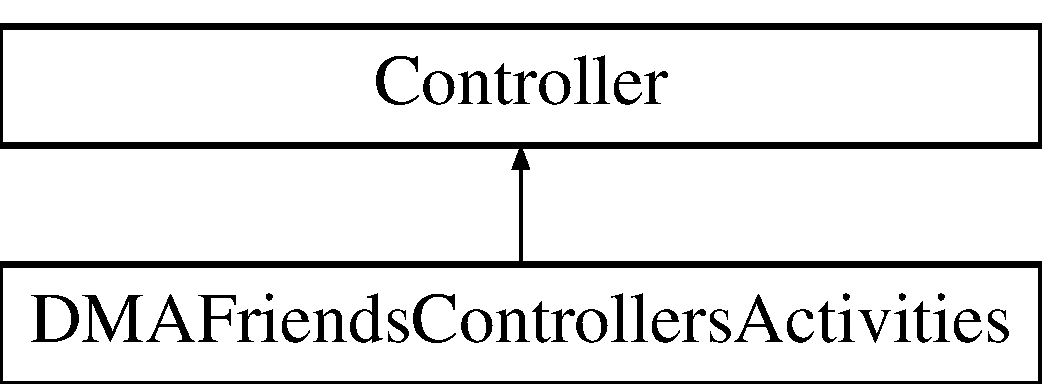
\includegraphics[height=2.000000cm]{d4/d37/classDMA_1_1Friends_1_1Controllers_1_1Activities}
\end{center}
\end{figure}
\subsection*{Public Attributes}
\begin{DoxyCompactItemize}
\item 
{\bfseries \$implement}
\item 
\hypertarget{classDMA_1_1Friends_1_1Controllers_1_1Activities_a05bd364a981c519d8288a80a0bf816d7}{{\bfseries \$form\-Config} = 'config\-\_\-form.\-yaml'}\label{classDMA_1_1Friends_1_1Controllers_1_1Activities_a05bd364a981c519d8288a80a0bf816d7}

\item 
\hypertarget{classDMA_1_1Friends_1_1Controllers_1_1Activities_ac9c246da820ff83a1c0ffe831421d26f}{{\bfseries \$list\-Config} = 'config\-\_\-list.\-yaml'}\label{classDMA_1_1Friends_1_1Controllers_1_1Activities_ac9c246da820ff83a1c0ffe831421d26f}

\end{DoxyCompactItemize}


\subsection{Detailed Description}
\hyperlink{classDMA_1_1Friends_1_1Controllers_1_1Activities}{Activities} Back-\/end Controller 

\subsection{Member Data Documentation}
\hypertarget{classDMA_1_1Friends_1_1Controllers_1_1Activities_aff57941f0ab53e417ce578994badc87f}{\index{D\-M\-A\-::\-Friends\-::\-Controllers\-::\-Activities@{D\-M\-A\-::\-Friends\-::\-Controllers\-::\-Activities}!\$implement@{\$implement}}
\index{\$implement@{\$implement}!DMA::Friends::Controllers::Activities@{D\-M\-A\-::\-Friends\-::\-Controllers\-::\-Activities}}
\subsubsection[{\$implement}]{\setlength{\rightskip}{0pt plus 5cm}D\-M\-A\textbackslash{}\-Friends\textbackslash{}\-Controllers\textbackslash{}\-Activities\-::\$implement}}\label{classDMA_1_1Friends_1_1Controllers_1_1Activities_aff57941f0ab53e417ce578994badc87f}
{\bfseries Initial value\-:}
\begin{DoxyCode}
= [
        \textcolor{stringliteral}{'Backend.Behaviors.FormController'},
        \textcolor{stringliteral}{'Backend.Behaviors.ListController'}
    ]
\end{DoxyCode}


The documentation for this class was generated from the following file\-:\begin{DoxyCompactItemize}
\item 
controllers/Activities.\-php\end{DoxyCompactItemize}

\hypertarget{classDMA_1_1Friends_1_1Models_1_1Activity}{\section{D\+M\+A\textbackslash{}Friends\textbackslash{}Models\textbackslash{}Activity Class Reference}
\label{classDMA_1_1Friends_1_1Models_1_1Activity}\index{D\+M\+A\textbackslash{}\+Friends\textbackslash{}\+Models\textbackslash{}\+Activity@{D\+M\+A\textbackslash{}\+Friends\textbackslash{}\+Models\textbackslash{}\+Activity}}
}
Inheritance diagram for D\+M\+A\textbackslash{}Friends\textbackslash{}Models\textbackslash{}Activity\+:\begin{figure}[H]
\begin{center}
\leavevmode
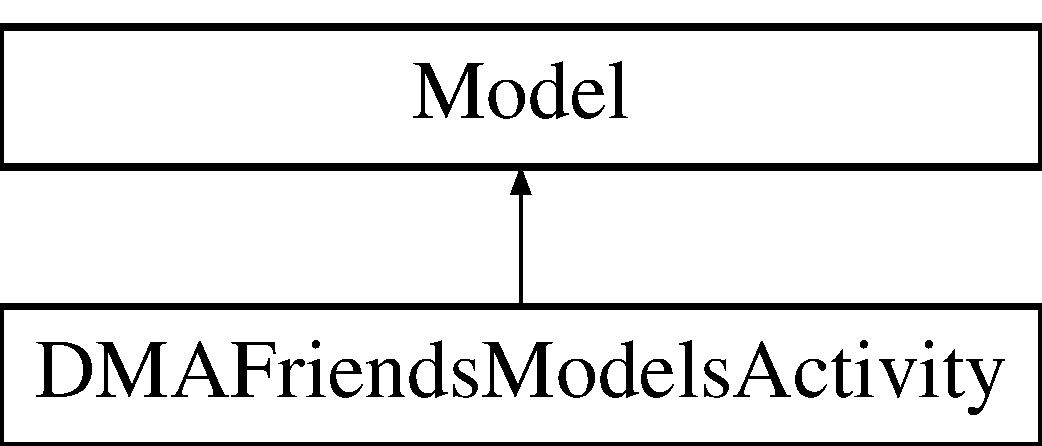
\includegraphics[height=2.000000cm]{dc/d8c/classDMA_1_1Friends_1_1Models_1_1Activity}
\end{center}
\end{figure}
\subsection*{Public Member Functions}
\begin{DoxyCompactItemize}
\item 
\hyperlink{classDMA_1_1Friends_1_1Models_1_1Activity_ade0ffca24448c217def365d104e52866}{set\+Time\+Restriction\+Data\+Attribute} (\$value)
\item 
\hyperlink{classDMA_1_1Friends_1_1Models_1_1Activity_a98a904c739aca30f2a26152a481164b6}{get\+Time\+Restriction\+Data\+Attribute} (\$value)
\item 
\hyperlink{classDMA_1_1Friends_1_1Models_1_1Activity_acd3f12824d95be07b5221cdc9d64abf7}{scope\+Is\+Active} (\$query)
\item 
\hyperlink{classDMA_1_1Friends_1_1Models_1_1Activity_a9bb36aab36ff22a29b2a594617dd591c}{scopefind\+Code} (\$query, \$code)
\item 
\hyperlink{classDMA_1_1Friends_1_1Models_1_1Activity_aa17825817b73d3073e37d5e2c0933003}{scope\+Find\+Activity\+Type} (\$query, \$type)
\item 
\hyperlink{classDMA_1_1Friends_1_1Models_1_1Activity_a5a533a3f638f99d1dd0a8e0550def49e}{scopefind\+Wordpress} (\$query, \$id)
\item 
\hyperlink{classDMA_1_1Friends_1_1Models_1_1Activity_a03415578b3f688ecd26d27d9254d23ab}{get\+Time\+Ago\+Attribute} (\$value)
\end{DoxyCompactItemize}
\subsection*{Public Attributes}
\begin{DoxyCompactItemize}
\item 
const \hyperlink{classDMA_1_1Friends_1_1Models_1_1Activity_ab9dd8b18c4810beabdcf8e45039913c8}{T\+I\+M\+E\+\_\+\+R\+E\+S\+T\+R\+I\+C\+T\+\_\+\+N\+O\+N\+E} = 0
\item 
const \hyperlink{classDMA_1_1Friends_1_1Models_1_1Activity_ac78040e8784e02c2d1bcce5221ac6cb8}{T\+I\+M\+E\+\_\+\+R\+E\+S\+T\+R\+I\+C\+T\+\_\+\+H\+O\+U\+R\+S} = 1
\item 
const \hyperlink{classDMA_1_1Friends_1_1Models_1_1Activity_a71b85478f20cda144aeffe010364a0f7}{T\+I\+M\+E\+\_\+\+R\+E\+S\+T\+R\+I\+C\+T\+\_\+\+D\+A\+Y\+S} = 2
\item 
\hypertarget{classDMA_1_1Friends_1_1Models_1_1Activity_a2ded517047c73d831aef535c8adc6690}{{\bfseries \$table} = 'dma\+\_\+friends\+\_\+activities'}\label{classDMA_1_1Friends_1_1Models_1_1Activity_a2ded517047c73d831aef535c8adc6690}

\item 
{\bfseries \$rules}
\item 
{\bfseries \$has\+Many}
\item 
{\bfseries \$belongs\+To\+Many}
\item 
{\bfseries \$attach\+One}
\item 
{\bfseries \$morph\+Many}
\item 
{\bfseries \$morph\+To\+Many}
\end{DoxyCompactItemize}
\subsection*{Protected Attributes}
\begin{DoxyCompactItemize}
\item 
\hypertarget{classDMA_1_1Friends_1_1Models_1_1Activity_ac82a10f722788b5c1c7a5295e1ac10c2}{{\bfseries \$guarded} = \mbox{[}'$\ast$'\mbox{]}}\label{classDMA_1_1Friends_1_1Models_1_1Activity_ac82a10f722788b5c1c7a5295e1ac10c2}

\item 
\hypertarget{classDMA_1_1Friends_1_1Models_1_1Activity_ab2a7401215dff9dfd8b600247b12454a}{{\bfseries \$fillable} = \mbox{[}'touch'\mbox{]}}\label{classDMA_1_1Friends_1_1Models_1_1Activity_ab2a7401215dff9dfd8b600247b12454a}

\item 
\hypertarget{classDMA_1_1Friends_1_1Models_1_1Activity_afe94503fbf177345e4bf0b1625dee499}{{\bfseries \$dates} = \mbox{[}'date\+\_\+begin', 'date\+\_\+end'\mbox{]}}\label{classDMA_1_1Friends_1_1Models_1_1Activity_afe94503fbf177345e4bf0b1625dee499}

\end{DoxyCompactItemize}


\subsection{Detailed Description}
\hyperlink{classDMA_1_1Friends_1_1Models_1_1Activity}{Activity} Model

N\+O\+T\+E\+: Time restrictions conform to the I\+S\+O-\/8601 numeric representation of the day of the week where 1 (for Monday) through 7 (for Sunday) see \href{http://php.net/manual/en/function.date.php}{\tt P\+H\+P's Date Manual} 

\subsection{Member Function Documentation}
\hypertarget{classDMA_1_1Friends_1_1Models_1_1Activity_a03415578b3f688ecd26d27d9254d23ab}{\index{D\+M\+A\+::\+Friends\+::\+Models\+::\+Activity@{D\+M\+A\+::\+Friends\+::\+Models\+::\+Activity}!get\+Time\+Ago\+Attribute@{get\+Time\+Ago\+Attribute}}
\index{get\+Time\+Ago\+Attribute@{get\+Time\+Ago\+Attribute}!D\+M\+A\+::\+Friends\+::\+Models\+::\+Activity@{D\+M\+A\+::\+Friends\+::\+Models\+::\+Activity}}
\subsubsection[{get\+Time\+Ago\+Attribute}]{\setlength{\rightskip}{0pt plus 5cm}D\+M\+A\textbackslash{}\+Friends\textbackslash{}\+Models\textbackslash{}\+Activity\+::get\+Time\+Ago\+Attribute (
\begin{DoxyParamCaption}
\item[{}]{\$value}
\end{DoxyParamCaption}
)}}\label{classDMA_1_1Friends_1_1Models_1_1Activity_a03415578b3f688ecd26d27d9254d23ab}
Mutator function to return the pivot timestamp as time ago \begin{DoxyReturn}{Returns}
string The time since the badge was earned 
\end{DoxyReturn}

\begin{DoxyCode}
137     \{
138         \textcolor{keywordflow}{if} (!isset($this->pivot->created\_at)) \textcolor{keywordflow}{return} null;
139 
140         $timeAgo = \textcolor{keyword}{new} TimeAgo;
141         \textcolor{keywordflow}{return} $timeAgo->get($this->pivot->created\_at);
142     \}
\end{DoxyCode}
\hypertarget{classDMA_1_1Friends_1_1Models_1_1Activity_a98a904c739aca30f2a26152a481164b6}{\index{D\+M\+A\+::\+Friends\+::\+Models\+::\+Activity@{D\+M\+A\+::\+Friends\+::\+Models\+::\+Activity}!get\+Time\+Restriction\+Data\+Attribute@{get\+Time\+Restriction\+Data\+Attribute}}
\index{get\+Time\+Restriction\+Data\+Attribute@{get\+Time\+Restriction\+Data\+Attribute}!D\+M\+A\+::\+Friends\+::\+Models\+::\+Activity@{D\+M\+A\+::\+Friends\+::\+Models\+::\+Activity}}
\subsubsection[{get\+Time\+Restriction\+Data\+Attribute}]{\setlength{\rightskip}{0pt plus 5cm}D\+M\+A\textbackslash{}\+Friends\textbackslash{}\+Models\textbackslash{}\+Activity\+::get\+Time\+Restriction\+Data\+Attribute (
\begin{DoxyParamCaption}
\item[{}]{\$value}
\end{DoxyParamCaption}
)}}\label{classDMA_1_1Friends_1_1Models_1_1Activity_a98a904c739aca30f2a26152a481164b6}
Accessor to unserialize time\+\_\+restriction\+\_\+data attribute 
\begin{DoxyCode}
93     \{
94         \textcolor{keywordflow}{return} unserialize($value);
95     \}
\end{DoxyCode}
\hypertarget{classDMA_1_1Friends_1_1Models_1_1Activity_aa17825817b73d3073e37d5e2c0933003}{\index{D\+M\+A\+::\+Friends\+::\+Models\+::\+Activity@{D\+M\+A\+::\+Friends\+::\+Models\+::\+Activity}!scope\+Find\+Activity\+Type@{scope\+Find\+Activity\+Type}}
\index{scope\+Find\+Activity\+Type@{scope\+Find\+Activity\+Type}!D\+M\+A\+::\+Friends\+::\+Models\+::\+Activity@{D\+M\+A\+::\+Friends\+::\+Models\+::\+Activity}}
\subsubsection[{scope\+Find\+Activity\+Type}]{\setlength{\rightskip}{0pt plus 5cm}D\+M\+A\textbackslash{}\+Friends\textbackslash{}\+Models\textbackslash{}\+Activity\+::scope\+Find\+Activity\+Type (
\begin{DoxyParamCaption}
\item[{}]{\$query, }
\item[{}]{\$type}
\end{DoxyParamCaption}
)}}\label{classDMA_1_1Friends_1_1Models_1_1Activity_aa17825817b73d3073e37d5e2c0933003}
Find activities by activity type 
\begin{DoxyCode}
119     \{
120         \textcolor{keywordflow}{return} $query->where(\textcolor{stringliteral}{'activity\_type'}, $type)
121             ->isActive();
122     \}
\end{DoxyCode}
\hypertarget{classDMA_1_1Friends_1_1Models_1_1Activity_a9bb36aab36ff22a29b2a594617dd591c}{\index{D\+M\+A\+::\+Friends\+::\+Models\+::\+Activity@{D\+M\+A\+::\+Friends\+::\+Models\+::\+Activity}!scopefind\+Code@{scopefind\+Code}}
\index{scopefind\+Code@{scopefind\+Code}!D\+M\+A\+::\+Friends\+::\+Models\+::\+Activity@{D\+M\+A\+::\+Friends\+::\+Models\+::\+Activity}}
\subsubsection[{scopefind\+Code}]{\setlength{\rightskip}{0pt plus 5cm}D\+M\+A\textbackslash{}\+Friends\textbackslash{}\+Models\textbackslash{}\+Activity\+::scopefind\+Code (
\begin{DoxyParamCaption}
\item[{}]{\$query, }
\item[{}]{\$code}
\end{DoxyParamCaption}
)}}\label{classDMA_1_1Friends_1_1Models_1_1Activity_a9bb36aab36ff22a29b2a594617dd591c}
Find an activity by its activity code 
\begin{DoxyCode}
110     \{
111         \textcolor{keywordflow}{return} $query->where(\textcolor{stringliteral}{'activity\_code'}, $code)
112             ->isActive();
113     \}
\end{DoxyCode}
\hypertarget{classDMA_1_1Friends_1_1Models_1_1Activity_a5a533a3f638f99d1dd0a8e0550def49e}{\index{D\+M\+A\+::\+Friends\+::\+Models\+::\+Activity@{D\+M\+A\+::\+Friends\+::\+Models\+::\+Activity}!scopefind\+Wordpress@{scopefind\+Wordpress}}
\index{scopefind\+Wordpress@{scopefind\+Wordpress}!D\+M\+A\+::\+Friends\+::\+Models\+::\+Activity@{D\+M\+A\+::\+Friends\+::\+Models\+::\+Activity}}
\subsubsection[{scopefind\+Wordpress}]{\setlength{\rightskip}{0pt plus 5cm}D\+M\+A\textbackslash{}\+Friends\textbackslash{}\+Models\textbackslash{}\+Activity\+::scopefind\+Wordpress (
\begin{DoxyParamCaption}
\item[{}]{\$query, }
\item[{}]{\$id}
\end{DoxyParamCaption}
)}}\label{classDMA_1_1Friends_1_1Models_1_1Activity_a5a533a3f638f99d1dd0a8e0550def49e}
Find activities by a wordpress id if they where imported 
\begin{DoxyCode}
128     \{   
129         \textcolor{keywordflow}{return} $query->where(\textcolor{stringliteral}{'wordpress\_id'}, $id);
130     \}  
\end{DoxyCode}
\hypertarget{classDMA_1_1Friends_1_1Models_1_1Activity_acd3f12824d95be07b5221cdc9d64abf7}{\index{D\+M\+A\+::\+Friends\+::\+Models\+::\+Activity@{D\+M\+A\+::\+Friends\+::\+Models\+::\+Activity}!scope\+Is\+Active@{scope\+Is\+Active}}
\index{scope\+Is\+Active@{scope\+Is\+Active}!D\+M\+A\+::\+Friends\+::\+Models\+::\+Activity@{D\+M\+A\+::\+Friends\+::\+Models\+::\+Activity}}
\subsubsection[{scope\+Is\+Active}]{\setlength{\rightskip}{0pt plus 5cm}D\+M\+A\textbackslash{}\+Friends\textbackslash{}\+Models\textbackslash{}\+Activity\+::scope\+Is\+Active (
\begin{DoxyParamCaption}
\item[{}]{\$query}
\end{DoxyParamCaption}
)}}\label{classDMA_1_1Friends_1_1Models_1_1Activity_acd3f12824d95be07b5221cdc9d64abf7}
Return only activities that are active 
\begin{DoxyCode}
101     \{
102         \textcolor{keywordflow}{return} $query->where(\textcolor{stringliteral}{'is\_published'}, \textcolor{charliteral}{'='}, 1)
103             ->where(\textcolor{stringliteral}{'is\_archived'}, \textcolor{stringliteral}{'<>'}, 1);
104     \}
\end{DoxyCode}
\hypertarget{classDMA_1_1Friends_1_1Models_1_1Activity_ade0ffca24448c217def365d104e52866}{\index{D\+M\+A\+::\+Friends\+::\+Models\+::\+Activity@{D\+M\+A\+::\+Friends\+::\+Models\+::\+Activity}!set\+Time\+Restriction\+Data\+Attribute@{set\+Time\+Restriction\+Data\+Attribute}}
\index{set\+Time\+Restriction\+Data\+Attribute@{set\+Time\+Restriction\+Data\+Attribute}!D\+M\+A\+::\+Friends\+::\+Models\+::\+Activity@{D\+M\+A\+::\+Friends\+::\+Models\+::\+Activity}}
\subsubsection[{set\+Time\+Restriction\+Data\+Attribute}]{\setlength{\rightskip}{0pt plus 5cm}D\+M\+A\textbackslash{}\+Friends\textbackslash{}\+Models\textbackslash{}\+Activity\+::set\+Time\+Restriction\+Data\+Attribute (
\begin{DoxyParamCaption}
\item[{}]{\$value}
\end{DoxyParamCaption}
)}}\label{classDMA_1_1Friends_1_1Models_1_1Activity_ade0ffca24448c217def365d104e52866}
Mutator to ensure time\+\_\+restriction\+\_\+data is serialized 
\begin{DoxyCode}
81     \{
82         \textcolor{keywordflow}{if} (is\_array($value)) \{
83             $value = serialize($value);
84         \}
85 
86         $this->attributes[\textcolor{stringliteral}{'time\_restriction\_data'}] = $value;
87     \}
\end{DoxyCode}


\subsection{Member Data Documentation}
\hypertarget{classDMA_1_1Friends_1_1Models_1_1Activity_a9911cb733cbc863cc1bdccde254404b5}{\index{D\+M\+A\+::\+Friends\+::\+Models\+::\+Activity@{D\+M\+A\+::\+Friends\+::\+Models\+::\+Activity}!\$attach\+One@{\$attach\+One}}
\index{\$attach\+One@{\$attach\+One}!D\+M\+A\+::\+Friends\+::\+Models\+::\+Activity@{D\+M\+A\+::\+Friends\+::\+Models\+::\+Activity}}
\subsubsection[{\$attach\+One}]{\setlength{\rightskip}{0pt plus 5cm}D\+M\+A\textbackslash{}\+Friends\textbackslash{}\+Models\textbackslash{}\+Activity\+::\$attach\+One}}\label{classDMA_1_1Friends_1_1Models_1_1Activity_a9911cb733cbc863cc1bdccde254404b5}
{\bfseries Initial value\+:}
\begin{DoxyCode}
= [
        \textcolor{stringliteral}{'image'} => [\textcolor{stringliteral}{'System\(\backslash\)Models\(\backslash\)File'}]
\end{DoxyCode}
\hypertarget{classDMA_1_1Friends_1_1Models_1_1Activity_ae5245e6eb74228cd54d8ae77e5a9bb38}{\index{D\+M\+A\+::\+Friends\+::\+Models\+::\+Activity@{D\+M\+A\+::\+Friends\+::\+Models\+::\+Activity}!\$belongs\+To\+Many@{\$belongs\+To\+Many}}
\index{\$belongs\+To\+Many@{\$belongs\+To\+Many}!D\+M\+A\+::\+Friends\+::\+Models\+::\+Activity@{D\+M\+A\+::\+Friends\+::\+Models\+::\+Activity}}
\subsubsection[{\$belongs\+To\+Many}]{\setlength{\rightskip}{0pt plus 5cm}D\+M\+A\textbackslash{}\+Friends\textbackslash{}\+Models\textbackslash{}\+Activity\+::\$belongs\+To\+Many}}\label{classDMA_1_1Friends_1_1Models_1_1Activity_ae5245e6eb74228cd54d8ae77e5a9bb38}
{\bfseries Initial value\+:}
\begin{DoxyCode}
= [
        \textcolor{stringliteral}{'users'} => [\textcolor{stringliteral}{'RainLab\(\backslash\)User\(\backslash\)Models\(\backslash\)User'}, \textcolor{stringliteral}{'table'} => \textcolor{stringliteral}{'dma\_friends\_activity\_user'}
\end{DoxyCode}
\hypertarget{classDMA_1_1Friends_1_1Models_1_1Activity_a8b255e9889df95f8c702b72ed49ace25}{\index{D\+M\+A\+::\+Friends\+::\+Models\+::\+Activity@{D\+M\+A\+::\+Friends\+::\+Models\+::\+Activity}!\$has\+Many@{\$has\+Many}}
\index{\$has\+Many@{\$has\+Many}!D\+M\+A\+::\+Friends\+::\+Models\+::\+Activity@{D\+M\+A\+::\+Friends\+::\+Models\+::\+Activity}}
\subsubsection[{\$has\+Many}]{\setlength{\rightskip}{0pt plus 5cm}D\+M\+A\textbackslash{}\+Friends\textbackslash{}\+Models\textbackslash{}\+Activity\+::\$has\+Many}}\label{classDMA_1_1Friends_1_1Models_1_1Activity_a8b255e9889df95f8c702b72ed49ace25}
{\bfseries Initial value\+:}
\begin{DoxyCode}
= [
        \textcolor{stringliteral}{'steps'} => [\textcolor{stringliteral}{'DMA\(\backslash\)Friends\(\backslash\)Models\(\backslash\)Step'}, \textcolor{stringliteral}{'table'} => \textcolor{stringliteral}{'dma\_friends\_activity\_step'}],
    ]
\end{DoxyCode}
\hypertarget{classDMA_1_1Friends_1_1Models_1_1Activity_a192fdaacf609961b7a436d2b967dfd60}{\index{D\+M\+A\+::\+Friends\+::\+Models\+::\+Activity@{D\+M\+A\+::\+Friends\+::\+Models\+::\+Activity}!\$morph\+Many@{\$morph\+Many}}
\index{\$morph\+Many@{\$morph\+Many}!D\+M\+A\+::\+Friends\+::\+Models\+::\+Activity@{D\+M\+A\+::\+Friends\+::\+Models\+::\+Activity}}
\subsubsection[{\$morph\+Many}]{\setlength{\rightskip}{0pt plus 5cm}D\+M\+A\textbackslash{}\+Friends\textbackslash{}\+Models\textbackslash{}\+Activity\+::\$morph\+Many}}\label{classDMA_1_1Friends_1_1Models_1_1Activity_a192fdaacf609961b7a436d2b967dfd60}
{\bfseries Initial value\+:}
\begin{DoxyCode}
= [ 
        \textcolor{stringliteral}{'activityLogs'}  => [\textcolor{stringliteral}{'DMA\(\backslash\)Friends\(\backslash\)Models\(\backslash\)ActivityLog'}, \textcolor{stringliteral}{'name'} => \textcolor{stringliteral}{'object'}],
    ]
\end{DoxyCode}
\hypertarget{classDMA_1_1Friends_1_1Models_1_1Activity_a5cfb1d646716be755dcdb6ddb3ab16b1}{\index{D\+M\+A\+::\+Friends\+::\+Models\+::\+Activity@{D\+M\+A\+::\+Friends\+::\+Models\+::\+Activity}!\$morph\+To\+Many@{\$morph\+To\+Many}}
\index{\$morph\+To\+Many@{\$morph\+To\+Many}!D\+M\+A\+::\+Friends\+::\+Models\+::\+Activity@{D\+M\+A\+::\+Friends\+::\+Models\+::\+Activity}}
\subsubsection[{\$morph\+To\+Many}]{\setlength{\rightskip}{0pt plus 5cm}D\+M\+A\textbackslash{}\+Friends\textbackslash{}\+Models\textbackslash{}\+Activity\+::\$morph\+To\+Many}}\label{classDMA_1_1Friends_1_1Models_1_1Activity_a5cfb1d646716be755dcdb6ddb3ab16b1}
{\bfseries Initial value\+:}
\begin{DoxyCode}
= [
        \textcolor{stringliteral}{'categories'}    => [\textcolor{stringliteral}{'DMA\(\backslash\)Friends\(\backslash\)Models\(\backslash\)Category'}, \textcolor{stringliteral}{'name'} => \textcolor{stringliteral}{'object'}
\end{DoxyCode}
\hypertarget{classDMA_1_1Friends_1_1Models_1_1Activity_a0b92e75aa8d92e2d3c9b24f54cd813bc}{\index{D\+M\+A\+::\+Friends\+::\+Models\+::\+Activity@{D\+M\+A\+::\+Friends\+::\+Models\+::\+Activity}!\$rules@{\$rules}}
\index{\$rules@{\$rules}!D\+M\+A\+::\+Friends\+::\+Models\+::\+Activity@{D\+M\+A\+::\+Friends\+::\+Models\+::\+Activity}}
\subsubsection[{\$rules}]{\setlength{\rightskip}{0pt plus 5cm}D\+M\+A\textbackslash{}\+Friends\textbackslash{}\+Models\textbackslash{}\+Activity\+::\$rules}}\label{classDMA_1_1Friends_1_1Models_1_1Activity_a0b92e75aa8d92e2d3c9b24f54cd813bc}
{\bfseries Initial value\+:}
\begin{DoxyCode}
= [ 
        \textcolor{stringliteral}{'title'}         => \textcolor{stringliteral}{'required'}
\end{DoxyCode}
\hypertarget{classDMA_1_1Friends_1_1Models_1_1Activity_a71b85478f20cda144aeffe010364a0f7}{\index{D\+M\+A\+::\+Friends\+::\+Models\+::\+Activity@{D\+M\+A\+::\+Friends\+::\+Models\+::\+Activity}!T\+I\+M\+E\+\_\+\+R\+E\+S\+T\+R\+I\+C\+T\+\_\+\+D\+A\+Y\+S@{T\+I\+M\+E\+\_\+\+R\+E\+S\+T\+R\+I\+C\+T\+\_\+\+D\+A\+Y\+S}}
\index{T\+I\+M\+E\+\_\+\+R\+E\+S\+T\+R\+I\+C\+T\+\_\+\+D\+A\+Y\+S@{T\+I\+M\+E\+\_\+\+R\+E\+S\+T\+R\+I\+C\+T\+\_\+\+D\+A\+Y\+S}!D\+M\+A\+::\+Friends\+::\+Models\+::\+Activity@{D\+M\+A\+::\+Friends\+::\+Models\+::\+Activity}}
\subsubsection[{T\+I\+M\+E\+\_\+\+R\+E\+S\+T\+R\+I\+C\+T\+\_\+\+D\+A\+Y\+S}]{\setlength{\rightskip}{0pt plus 5cm}const D\+M\+A\textbackslash{}\+Friends\textbackslash{}\+Models\textbackslash{}\+Activity\+::\+T\+I\+M\+E\+\_\+\+R\+E\+S\+T\+R\+I\+C\+T\+\_\+\+D\+A\+Y\+S = 2}}\label{classDMA_1_1Friends_1_1Models_1_1Activity_a71b85478f20cda144aeffe010364a0f7}
A time restriction is set by a date range \hypertarget{classDMA_1_1Friends_1_1Models_1_1Activity_ac78040e8784e02c2d1bcce5221ac6cb8}{\index{D\+M\+A\+::\+Friends\+::\+Models\+::\+Activity@{D\+M\+A\+::\+Friends\+::\+Models\+::\+Activity}!T\+I\+M\+E\+\_\+\+R\+E\+S\+T\+R\+I\+C\+T\+\_\+\+H\+O\+U\+R\+S@{T\+I\+M\+E\+\_\+\+R\+E\+S\+T\+R\+I\+C\+T\+\_\+\+H\+O\+U\+R\+S}}
\index{T\+I\+M\+E\+\_\+\+R\+E\+S\+T\+R\+I\+C\+T\+\_\+\+H\+O\+U\+R\+S@{T\+I\+M\+E\+\_\+\+R\+E\+S\+T\+R\+I\+C\+T\+\_\+\+H\+O\+U\+R\+S}!D\+M\+A\+::\+Friends\+::\+Models\+::\+Activity@{D\+M\+A\+::\+Friends\+::\+Models\+::\+Activity}}
\subsubsection[{T\+I\+M\+E\+\_\+\+R\+E\+S\+T\+R\+I\+C\+T\+\_\+\+H\+O\+U\+R\+S}]{\setlength{\rightskip}{0pt plus 5cm}const D\+M\+A\textbackslash{}\+Friends\textbackslash{}\+Models\textbackslash{}\+Activity\+::\+T\+I\+M\+E\+\_\+\+R\+E\+S\+T\+R\+I\+C\+T\+\_\+\+H\+O\+U\+R\+S = 1}}\label{classDMA_1_1Friends_1_1Models_1_1Activity_ac78040e8784e02c2d1bcce5221ac6cb8}
A time restriction is set by individual hours and days of the week \hypertarget{classDMA_1_1Friends_1_1Models_1_1Activity_ab9dd8b18c4810beabdcf8e45039913c8}{\index{D\+M\+A\+::\+Friends\+::\+Models\+::\+Activity@{D\+M\+A\+::\+Friends\+::\+Models\+::\+Activity}!T\+I\+M\+E\+\_\+\+R\+E\+S\+T\+R\+I\+C\+T\+\_\+\+N\+O\+N\+E@{T\+I\+M\+E\+\_\+\+R\+E\+S\+T\+R\+I\+C\+T\+\_\+\+N\+O\+N\+E}}
\index{T\+I\+M\+E\+\_\+\+R\+E\+S\+T\+R\+I\+C\+T\+\_\+\+N\+O\+N\+E@{T\+I\+M\+E\+\_\+\+R\+E\+S\+T\+R\+I\+C\+T\+\_\+\+N\+O\+N\+E}!D\+M\+A\+::\+Friends\+::\+Models\+::\+Activity@{D\+M\+A\+::\+Friends\+::\+Models\+::\+Activity}}
\subsubsection[{T\+I\+M\+E\+\_\+\+R\+E\+S\+T\+R\+I\+C\+T\+\_\+\+N\+O\+N\+E}]{\setlength{\rightskip}{0pt plus 5cm}const D\+M\+A\textbackslash{}\+Friends\textbackslash{}\+Models\textbackslash{}\+Activity\+::\+T\+I\+M\+E\+\_\+\+R\+E\+S\+T\+R\+I\+C\+T\+\_\+\+N\+O\+N\+E = 0}}\label{classDMA_1_1Friends_1_1Models_1_1Activity_ab9dd8b18c4810beabdcf8e45039913c8}
No time restriction set 

The documentation for this class was generated from the following file\+:\begin{DoxyCompactItemize}
\item 
models/Activity.\+php\end{DoxyCompactItemize}

\hypertarget{classDMA_1_1Friends_1_1Wordpress_1_1Activity}{}\section{D\+M\+A\textbackslash{}Friends\textbackslash{}Wordpress\textbackslash{}Activity Class Reference}
\label{classDMA_1_1Friends_1_1Wordpress_1_1Activity}\index{D\+M\+A\textbackslash{}\+Friends\textbackslash{}\+Wordpress\textbackslash{}\+Activity@{D\+M\+A\textbackslash{}\+Friends\textbackslash{}\+Wordpress\textbackslash{}\+Activity}}
Inheritance diagram for D\+M\+A\textbackslash{}Friends\textbackslash{}Wordpress\textbackslash{}Activity\+:\begin{figure}[H]
\begin{center}
\leavevmode
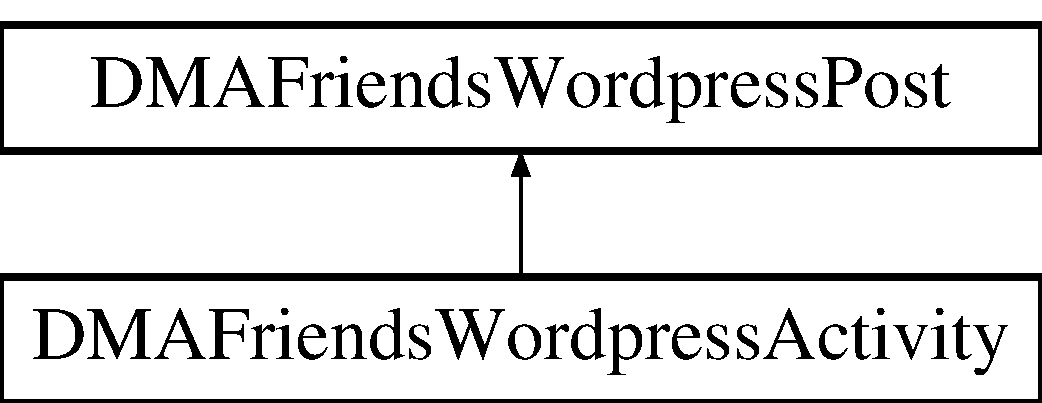
\includegraphics[height=2.000000cm]{de/d54/classDMA_1_1Friends_1_1Wordpress_1_1Activity}
\end{center}
\end{figure}
\subsection*{Public Attributes}
\begin{DoxyCompactItemize}
\item 
\hyperlink{classDMA_1_1Friends_1_1Wordpress_1_1Activity_a06a7b4fad854f04e2282f92e9829c3d3}{\$post\+Type} = \textquotesingle{}activity\textquotesingle{}
\end{DoxyCompactItemize}
\subsection*{Additional Inherited Members}


\subsection{Member Data Documentation}
\hypertarget{classDMA_1_1Friends_1_1Wordpress_1_1Activity_a06a7b4fad854f04e2282f92e9829c3d3}{}\index{D\+M\+A\+::\+Friends\+::\+Wordpress\+::\+Activity@{D\+M\+A\+::\+Friends\+::\+Wordpress\+::\+Activity}!\$post\+Type@{\$post\+Type}}
\index{\$post\+Type@{\$post\+Type}!D\+M\+A\+::\+Friends\+::\+Wordpress\+::\+Activity@{D\+M\+A\+::\+Friends\+::\+Wordpress\+::\+Activity}}
\subsubsection[{\$post\+Type}]{\setlength{\rightskip}{0pt plus 5cm}D\+M\+A\textbackslash{}\+Friends\textbackslash{}\+Wordpress\textbackslash{}\+Activity\+::\$post\+Type = \textquotesingle{}activity\textquotesingle{}}\label{classDMA_1_1Friends_1_1Wordpress_1_1Activity_a06a7b4fad854f04e2282f92e9829c3d3}
Override the default post type 

The documentation for this class was generated from the following file\+:\begin{DoxyCompactItemize}
\item 
wordpress/Activity.\+php\end{DoxyCompactItemize}

\hypertarget{classDMA_1_1Friends_1_1Models_1_1ActivityLog}{\section{D\-M\-A\textbackslash{}Friends\textbackslash{}Models\textbackslash{}Activity\-Log Class Reference}
\label{classDMA_1_1Friends_1_1Models_1_1ActivityLog}\index{D\-M\-A\textbackslash{}\-Friends\textbackslash{}\-Models\textbackslash{}\-Activity\-Log@{D\-M\-A\textbackslash{}\-Friends\textbackslash{}\-Models\textbackslash{}\-Activity\-Log}}
}
Inheritance diagram for D\-M\-A\textbackslash{}Friends\textbackslash{}Models\textbackslash{}Activity\-Log\-:\begin{figure}[H]
\begin{center}
\leavevmode
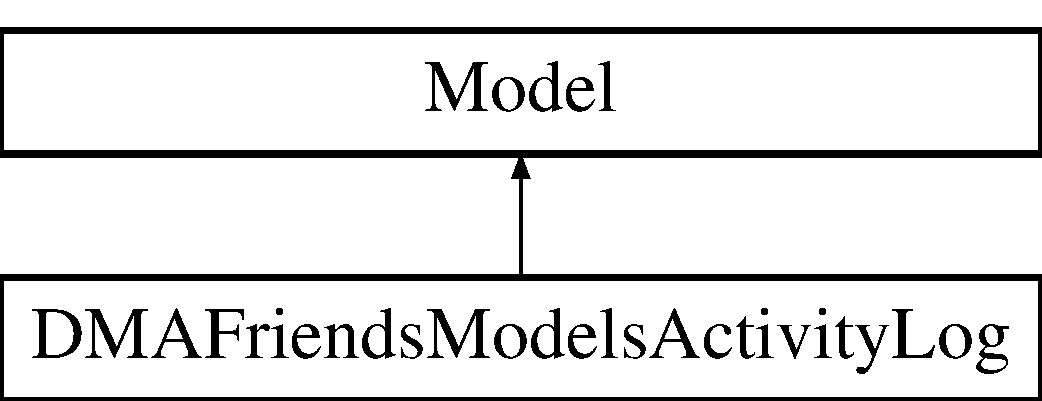
\includegraphics[height=2.000000cm]{d8/ddf/classDMA_1_1Friends_1_1Models_1_1ActivityLog}
\end{center}
\end{figure}
\subsection*{Public Attributes}
\begin{DoxyCompactItemize}
\item 
\hypertarget{classDMA_1_1Friends_1_1Models_1_1ActivityLog_a231d21bb93f9c0079c3f5cf51369d0c1}{{\bfseries \$table} = 'dma\-\_\-friends\-\_\-activity\-\_\-logs'}\label{classDMA_1_1Friends_1_1Models_1_1ActivityLog_a231d21bb93f9c0079c3f5cf51369d0c1}

\item 
\hypertarget{classDMA_1_1Friends_1_1Models_1_1ActivityLog_a11055e835c6bf48f58e019267dd469a2}{{\bfseries \$timestamps} = false}\label{classDMA_1_1Friends_1_1Models_1_1ActivityLog_a11055e835c6bf48f58e019267dd469a2}

\item 
\hyperlink{classDMA_1_1Friends_1_1Models_1_1ActivityLog_aa60b5fe0e1e7c254827bfa35c69aef9d}{\$action\-Types}
\item 
{\bfseries \$belongs\-To}
\item 
{\bfseries \$morph\-To}
\end{DoxyCompactItemize}
\subsection*{Protected Attributes}
\begin{DoxyCompactItemize}
\item 
\hypertarget{classDMA_1_1Friends_1_1Models_1_1ActivityLog_a93009970cd65274bd1b7031986a53a52}{{\bfseries \$dates} = \mbox{[}'timestamp'\mbox{]}}\label{classDMA_1_1Friends_1_1Models_1_1ActivityLog_a93009970cd65274bd1b7031986a53a52}

\item 
\hypertarget{classDMA_1_1Friends_1_1Models_1_1ActivityLog_a1ee25a9d84f85dd39fbb9e5a5b005515}{{\bfseries \$guarded} = \mbox{[}'$\ast$'\mbox{]}}\label{classDMA_1_1Friends_1_1Models_1_1ActivityLog_a1ee25a9d84f85dd39fbb9e5a5b005515}

\item 
\hypertarget{classDMA_1_1Friends_1_1Models_1_1ActivityLog_ab42303e736f297bda15a97fd903b8d4d}{{\bfseries \$fillable} = \mbox{[}$\,$\mbox{]}}\label{classDMA_1_1Friends_1_1Models_1_1ActivityLog_ab42303e736f297bda15a97fd903b8d4d}

\item 
{\bfseries \$rules}
\end{DoxyCompactItemize}


\subsection{Detailed Description}
\hyperlink{classDMA_1_1Friends_1_1Models_1_1ActivityLog}{Activity\-Log} Model 

\subsection{Member Data Documentation}
\hypertarget{classDMA_1_1Friends_1_1Models_1_1ActivityLog_aa60b5fe0e1e7c254827bfa35c69aef9d}{\index{D\-M\-A\-::\-Friends\-::\-Models\-::\-Activity\-Log@{D\-M\-A\-::\-Friends\-::\-Models\-::\-Activity\-Log}!\$action\-Types@{\$action\-Types}}
\index{\$action\-Types@{\$action\-Types}!DMA::Friends::Models::ActivityLog@{D\-M\-A\-::\-Friends\-::\-Models\-::\-Activity\-Log}}
\subsubsection[{\$action\-Types}]{\setlength{\rightskip}{0pt plus 5cm}D\-M\-A\textbackslash{}\-Friends\textbackslash{}\-Models\textbackslash{}\-Activity\-Log\-::\$action\-Types}}\label{classDMA_1_1Friends_1_1Models_1_1ActivityLog_aa60b5fe0e1e7c254827bfa35c69aef9d}
{\bfseries Initial value\-:}
\begin{DoxyCode}
= [
        \textcolor{stringliteral}{'activity'},
        \textcolor{stringliteral}{'artwork'},
        \textcolor{stringliteral}{'points'},
        \textcolor{stringliteral}{'reward'},
        \textcolor{stringliteral}{'unlocked'},
    ]
\end{DoxyCode}
The list of acceptable action types \hypertarget{classDMA_1_1Friends_1_1Models_1_1ActivityLog_aff637d41ffa73260e1ffc1788f5a98d7}{\index{D\-M\-A\-::\-Friends\-::\-Models\-::\-Activity\-Log@{D\-M\-A\-::\-Friends\-::\-Models\-::\-Activity\-Log}!\$belongs\-To@{\$belongs\-To}}
\index{\$belongs\-To@{\$belongs\-To}!DMA::Friends::Models::ActivityLog@{D\-M\-A\-::\-Friends\-::\-Models\-::\-Activity\-Log}}
\subsubsection[{\$belongs\-To}]{\setlength{\rightskip}{0pt plus 5cm}D\-M\-A\textbackslash{}\-Friends\textbackslash{}\-Models\textbackslash{}\-Activity\-Log\-::\$belongs\-To}}\label{classDMA_1_1Friends_1_1Models_1_1ActivityLog_aff637d41ffa73260e1ffc1788f5a98d7}
{\bfseries Initial value\-:}
\begin{DoxyCode}
= [
        \textcolor{stringliteral}{'user'} => [\textcolor{stringliteral}{'\(\backslash\)RainLab\(\backslash\)User\(\backslash\)Models\(\backslash\)User'}]
    ]
\end{DoxyCode}
\hypertarget{classDMA_1_1Friends_1_1Models_1_1ActivityLog_afaa82849e3e93bf41ac948658ac652ff}{\index{D\-M\-A\-::\-Friends\-::\-Models\-::\-Activity\-Log@{D\-M\-A\-::\-Friends\-::\-Models\-::\-Activity\-Log}!\$morph\-To@{\$morph\-To}}
\index{\$morph\-To@{\$morph\-To}!DMA::Friends::Models::ActivityLog@{D\-M\-A\-::\-Friends\-::\-Models\-::\-Activity\-Log}}
\subsubsection[{\$morph\-To}]{\setlength{\rightskip}{0pt plus 5cm}D\-M\-A\textbackslash{}\-Friends\textbackslash{}\-Models\textbackslash{}\-Activity\-Log\-::\$morph\-To}}\label{classDMA_1_1Friends_1_1Models_1_1ActivityLog_afaa82849e3e93bf41ac948658ac652ff}
{\bfseries Initial value\-:}
\begin{DoxyCode}
= [
        \textcolor{stringliteral}{'object'},
    ]
\end{DoxyCode}
\hypertarget{classDMA_1_1Friends_1_1Models_1_1ActivityLog_a0b8a60f69fd1fef78f71d538ca6f12e0}{\index{D\-M\-A\-::\-Friends\-::\-Models\-::\-Activity\-Log@{D\-M\-A\-::\-Friends\-::\-Models\-::\-Activity\-Log}!\$rules@{\$rules}}
\index{\$rules@{\$rules}!DMA::Friends::Models::ActivityLog@{D\-M\-A\-::\-Friends\-::\-Models\-::\-Activity\-Log}}
\subsubsection[{\$rules}]{\setlength{\rightskip}{0pt plus 5cm}D\-M\-A\textbackslash{}\-Friends\textbackslash{}\-Models\textbackslash{}\-Activity\-Log\-::\$rules\hspace{0.3cm}{\ttfamily [protected]}}}\label{classDMA_1_1Friends_1_1Models_1_1ActivityLog_a0b8a60f69fd1fef78f71d538ca6f12e0}
{\bfseries Initial value\-:}
\begin{DoxyCode}
= [
        \textcolor{stringliteral}{'message'}       => \textcolor{stringliteral}{'min:10'}
\end{DoxyCode}


The documentation for this class was generated from the following file\-:\begin{DoxyCompactItemize}
\item 
models/Activity\-Log.\-php\end{DoxyCompactItemize}

\hypertarget{classDMA_1_1Friends_1_1Wordpress_1_1ActivityLog}{\section{D\+M\+A\textbackslash{}Friends\textbackslash{}Wordpress\textbackslash{}Activity\+Log Class Reference}
\label{classDMA_1_1Friends_1_1Wordpress_1_1ActivityLog}\index{D\+M\+A\textbackslash{}\+Friends\textbackslash{}\+Wordpress\textbackslash{}\+Activity\+Log@{D\+M\+A\textbackslash{}\+Friends\textbackslash{}\+Wordpress\textbackslash{}\+Activity\+Log}}
}
Inheritance diagram for D\+M\+A\textbackslash{}Friends\textbackslash{}Wordpress\textbackslash{}Activity\+Log\+:\begin{figure}[H]
\begin{center}
\leavevmode
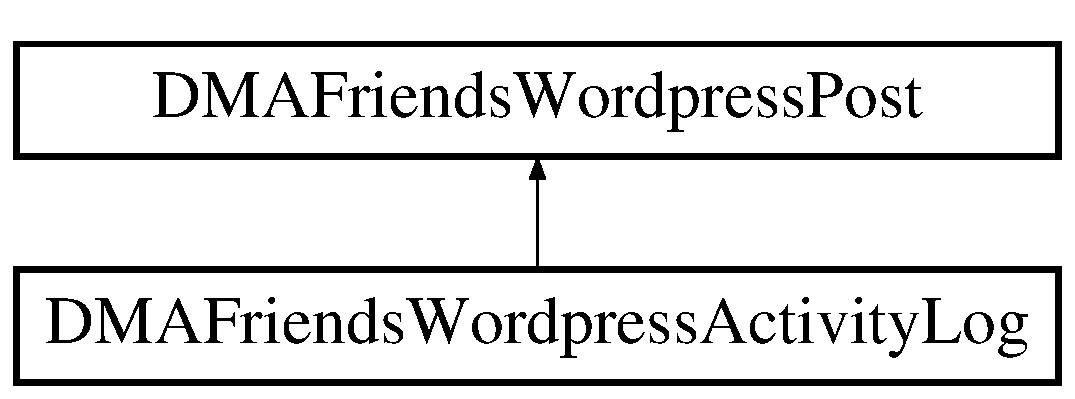
\includegraphics[height=2.000000cm]{d3/d37/classDMA_1_1Friends_1_1Wordpress_1_1ActivityLog}
\end{center}
\end{figure}
\subsection*{Public Member Functions}
\begin{DoxyCompactItemize}
\item 
\hyperlink{classDMA_1_1Friends_1_1Wordpress_1_1ActivityLog_a51567d47aa076394d865e890747f9832}{import} (\$limit=0)
\end{DoxyCompactItemize}
\subsection*{Additional Inherited Members}


\subsection{Member Function Documentation}
\hypertarget{classDMA_1_1Friends_1_1Wordpress_1_1ActivityLog_a51567d47aa076394d865e890747f9832}{\index{D\+M\+A\+::\+Friends\+::\+Wordpress\+::\+Activity\+Log@{D\+M\+A\+::\+Friends\+::\+Wordpress\+::\+Activity\+Log}!import@{import}}
\index{import@{import}!D\+M\+A\+::\+Friends\+::\+Wordpress\+::\+Activity\+Log@{D\+M\+A\+::\+Friends\+::\+Wordpress\+::\+Activity\+Log}}
\subsubsection[{import}]{\setlength{\rightskip}{0pt plus 5cm}D\+M\+A\textbackslash{}\+Friends\textbackslash{}\+Wordpress\textbackslash{}\+Activity\+Log\+::import (
\begin{DoxyParamCaption}
\item[{}]{\$limit = {\ttfamily 0}}
\end{DoxyParamCaption}
)}}\label{classDMA_1_1Friends_1_1Wordpress_1_1ActivityLog_a51567d47aa076394d865e890747f9832}
Import user accounts from wordpress


\begin{DoxyParams}[1]{Parameters}
int & {\em \$limit} & The amount of records to import at one time \\
\hline
\end{DoxyParams}

\begin{DoxyCode}
24     \{
25         $count  = 0;
26         $table  = $this->model->table;
27         $id     = (int)DB::table($table)->max(\textcolor{stringliteral}{'id'});
28 
29         $wordpressLogs = $this->db
30             ->table(\textcolor{stringliteral}{'wp\_badgeos\_logs'})
31             ->where(\textcolor{stringliteral}{'id'}, \textcolor{charliteral}{'>'}, $id)
32             ->orderBy(\textcolor{stringliteral}{'id'}, \textcolor{stringliteral}{'asc'})
33             ->limit($limit)
34             ->get();
35 
36         \textcolor{comment}{// Use dummy model to get action types}
37         $l = \textcolor{keyword}{new} \hyperlink{classDMA_1_1Friends_1_1Wordpress_1_1Post_a8a3df2e9db7f90d348d27ea9354176b1}{$this->model};
38 
39         \textcolor{keywordflow}{foreach} ($wordpressLogs as $wlog) \{
40 
41             \textcolor{keywordflow}{if} (!in\_array($wlog->action, $l->actionTypes)) \textcolor{keywordflow}{continue};
42 
43             $log                = \textcolor{keyword}{new} \hyperlink{classDMA_1_1Friends_1_1Wordpress_1_1Post_a8a3df2e9db7f90d348d27ea9354176b1}{$this->model};
44             $log->id            = $wlog->id;
45             $log->user\_id       = $wlog->user\_id;
46             $log->action        = $wlog->action;
47             $log->message       = $wlog->message;
48             $log->points\_earned = $wlog->points\_earned;
49             $log->total\_points  = $wlog->total\_points;
50             $log->timestamp     = $wlog->timestamp;
51             $log->timezone      = $wlog->timezone;
52     
53             \textcolor{keywordflow}{if} ($wlog->action == \textcolor{stringliteral}{'artwork'}) \{
54                 $log->artwork\_id = $wlog->object\_id;
55             \} \textcolor{keywordflow}{else} \{
56                 $log->object\_id = $wlog->object\_id;
57 
58                 $type = $this->db
59                     ->table(\textcolor{stringliteral}{'wp\_posts'})
60                     ->select(\textcolor{stringliteral}{'post\_type'})
61                     ->where(\textcolor{stringliteral}{'ID'}, $log->object\_id)
62                     ->first();
63 
64                 \textcolor{keywordflow}{if} ($type) \{
65                     $log->object\_type = $type->post\_type;
66                 \}   
67             \}   
68 
69             \textcolor{keywordflow}{if} ($log->save()) \{
70                 $count++;
71             \} 
72         \}  
73 
74         \textcolor{keywordflow}{return} $count;
75     \}
\end{DoxyCode}


The documentation for this class was generated from the following file\+:\begin{DoxyCompactItemize}
\item 
wordpress/Activity\+Log.\+php\end{DoxyCompactItemize}

\hypertarget{classDMA_1_1Friends_1_1Api_1_1ActivityLogResource}{\section{D\+M\+A\textbackslash{}Friends\textbackslash{}Api\textbackslash{}Activity\+Log\+Resource Class Reference}
\label{classDMA_1_1Friends_1_1Api_1_1ActivityLogResource}\index{D\+M\+A\textbackslash{}\+Friends\textbackslash{}\+Api\textbackslash{}\+Activity\+Log\+Resource@{D\+M\+A\textbackslash{}\+Friends\textbackslash{}\+Api\textbackslash{}\+Activity\+Log\+Resource}}
}
Inheritance diagram for D\+M\+A\textbackslash{}Friends\textbackslash{}Api\textbackslash{}Activity\+Log\+Resource\+:\begin{figure}[H]
\begin{center}
\leavevmode
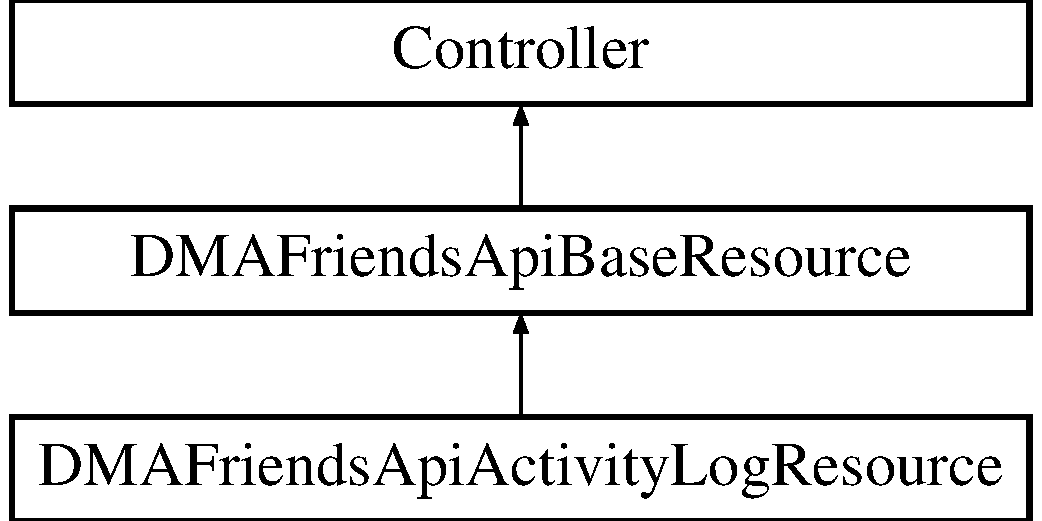
\includegraphics[height=3.000000cm]{d2/de6/classDMA_1_1Friends_1_1Api_1_1ActivityLogResource}
\end{center}
\end{figure}
\subsection*{Protected Attributes}
\begin{DoxyCompactItemize}
\item 
\hypertarget{classDMA_1_1Friends_1_1Api_1_1ActivityLogResource_abc7fd905609e3135075185ce7af02e43}{{\bfseries \$model} = '\textbackslash{}\hyperlink{classDMA_1_1Friends_1_1Models_1_1ActivityLog}{D\+M\+A\textbackslash{}\+Friends\textbackslash{}\+Models\textbackslash{}\+Activity\+Log}'}\label{classDMA_1_1Friends_1_1Api_1_1ActivityLogResource_abc7fd905609e3135075185ce7af02e43}

\end{DoxyCompactItemize}
\subsection*{Additional Inherited Members}


The documentation for this class was generated from the following file\+:\begin{DoxyCompactItemize}
\item 
api/Activity\+Log\+Resource.\+php\end{DoxyCompactItemize}

\hypertarget{classDMA_1_1Friends_1_1Controllers_1_1ActivityLogs}{\section{D\+M\+A\textbackslash{}Friends\textbackslash{}Controllers\textbackslash{}Activity\+Logs Class Reference}
\label{classDMA_1_1Friends_1_1Controllers_1_1ActivityLogs}\index{D\+M\+A\textbackslash{}\+Friends\textbackslash{}\+Controllers\textbackslash{}\+Activity\+Logs@{D\+M\+A\textbackslash{}\+Friends\textbackslash{}\+Controllers\textbackslash{}\+Activity\+Logs}}
}
Inheritance diagram for D\+M\+A\textbackslash{}Friends\textbackslash{}Controllers\textbackslash{}Activity\+Logs\+:\begin{figure}[H]
\begin{center}
\leavevmode
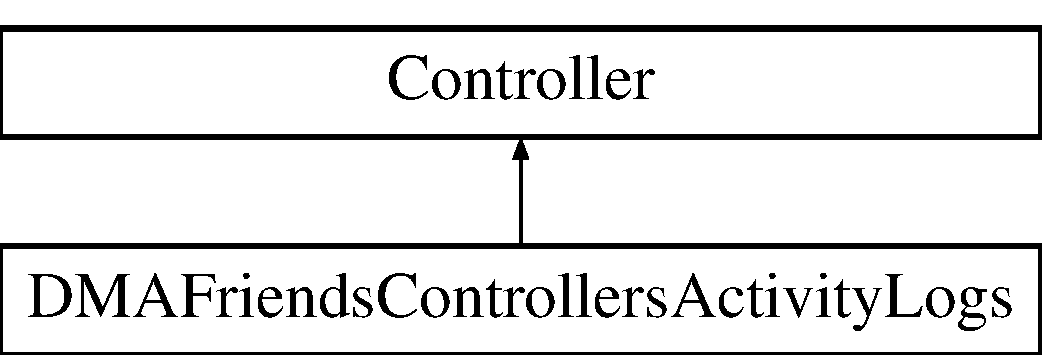
\includegraphics[height=2.000000cm]{d4/d23/classDMA_1_1Friends_1_1Controllers_1_1ActivityLogs}
\end{center}
\end{figure}
\subsection*{Public Attributes}
\begin{DoxyCompactItemize}
\item 
{\bfseries \$implement}
\item 
\hypertarget{classDMA_1_1Friends_1_1Controllers_1_1ActivityLogs_a2b07b2999d34d646303a3d70ade2da0a}{{\bfseries \$form\+Config} = 'config\+\_\+form.\+yaml'}\label{classDMA_1_1Friends_1_1Controllers_1_1ActivityLogs_a2b07b2999d34d646303a3d70ade2da0a}

\item 
\hypertarget{classDMA_1_1Friends_1_1Controllers_1_1ActivityLogs_a4f2d381656dbf1241a60f5b404a6230b}{{\bfseries \$list\+Config} = 'config\+\_\+list.\+yaml'}\label{classDMA_1_1Friends_1_1Controllers_1_1ActivityLogs_a4f2d381656dbf1241a60f5b404a6230b}

\end{DoxyCompactItemize}


\subsection{Detailed Description}
\hyperlink{classDMA_1_1Friends_1_1Controllers_1_1ActivityLogs}{Activity\+Logs} Back-\/end Controller 

\subsection{Member Data Documentation}
\hypertarget{classDMA_1_1Friends_1_1Controllers_1_1ActivityLogs_a9bbdc3717a05733011613af3108025fe}{\index{D\+M\+A\+::\+Friends\+::\+Controllers\+::\+Activity\+Logs@{D\+M\+A\+::\+Friends\+::\+Controllers\+::\+Activity\+Logs}!\$implement@{\$implement}}
\index{\$implement@{\$implement}!D\+M\+A\+::\+Friends\+::\+Controllers\+::\+Activity\+Logs@{D\+M\+A\+::\+Friends\+::\+Controllers\+::\+Activity\+Logs}}
\subsubsection[{\$implement}]{\setlength{\rightskip}{0pt plus 5cm}D\+M\+A\textbackslash{}\+Friends\textbackslash{}\+Controllers\textbackslash{}\+Activity\+Logs\+::\$implement}}\label{classDMA_1_1Friends_1_1Controllers_1_1ActivityLogs_a9bbdc3717a05733011613af3108025fe}
{\bfseries Initial value\+:}
\begin{DoxyCode}
= [
        \textcolor{stringliteral}{'Backend.Behaviors.FormController'},
        \textcolor{stringliteral}{'Backend.Behaviors.ListController'}
    ]
\end{DoxyCode}


The documentation for this class was generated from the following file\+:\begin{DoxyCompactItemize}
\item 
controllers/Activity\+Logs.\+php\end{DoxyCompactItemize}

\hypertarget{classDMA_1_1Friends_1_1Api_1_1ActivityLogTransformer}{}\section{D\+M\+A\textbackslash{}Friends\textbackslash{}Api\textbackslash{}Activity\+Log\+Transformer Class Reference}
\label{classDMA_1_1Friends_1_1Api_1_1ActivityLogTransformer}\index{D\+M\+A\textbackslash{}\+Friends\textbackslash{}\+Api\textbackslash{}\+Activity\+Log\+Transformer@{D\+M\+A\textbackslash{}\+Friends\textbackslash{}\+Api\textbackslash{}\+Activity\+Log\+Transformer}}
Inheritance diagram for D\+M\+A\textbackslash{}Friends\textbackslash{}Api\textbackslash{}Activity\+Log\+Transformer\+:\begin{figure}[H]
\begin{center}
\leavevmode
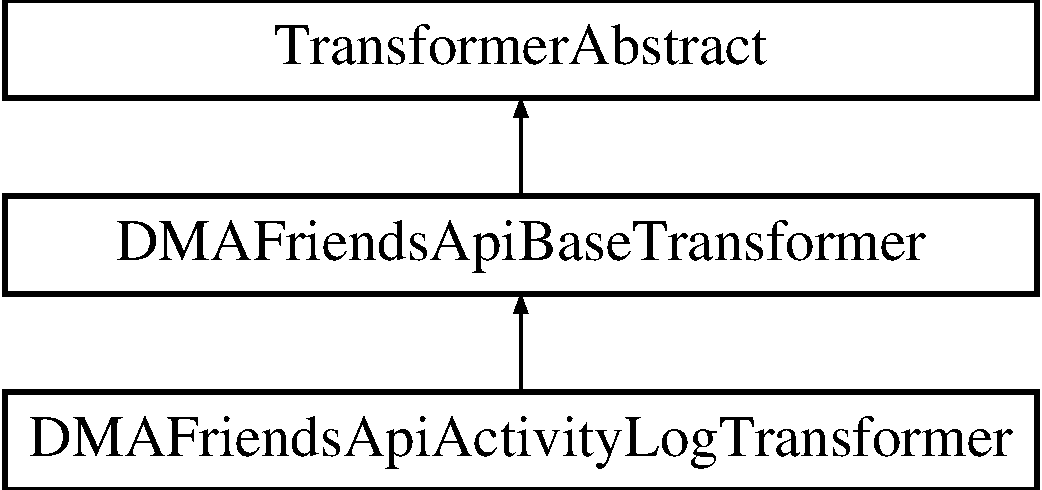
\includegraphics[height=3.000000cm]{d1/db3/classDMA_1_1Friends_1_1Api_1_1ActivityLogTransformer}
\end{center}
\end{figure}
\subsection*{Additional Inherited Members}


The documentation for this class was generated from the following file\+:\begin{DoxyCompactItemize}
\item 
api/Activity\+Log\+Resource.\+php\end{DoxyCompactItemize}

\hypertarget{classDMA_1_1Friends_1_1Classes_1_1ActivityProcessor}{\section{D\+M\+A\textbackslash{}Friends\textbackslash{}Classes\textbackslash{}Activity\+Processor Class Reference}
\label{classDMA_1_1Friends_1_1Classes_1_1ActivityProcessor}\index{D\+M\+A\textbackslash{}\+Friends\textbackslash{}\+Classes\textbackslash{}\+Activity\+Processor@{D\+M\+A\textbackslash{}\+Friends\textbackslash{}\+Classes\textbackslash{}\+Activity\+Processor}}
}
Inheritance diagram for D\+M\+A\textbackslash{}Friends\textbackslash{}Classes\textbackslash{}Activity\+Processor\+:\begin{figure}[H]
\begin{center}
\leavevmode
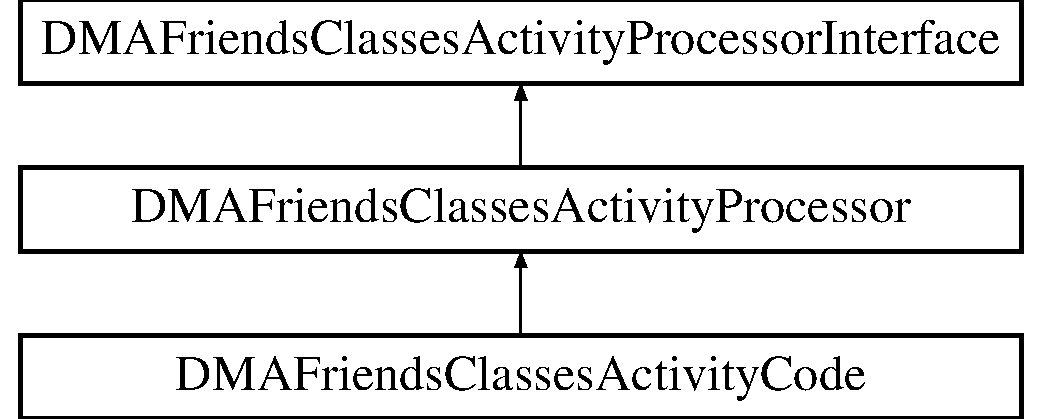
\includegraphics[height=3.000000cm]{db/d9c/classDMA_1_1Friends_1_1Classes_1_1ActivityProcessor}
\end{center}
\end{figure}
\subsection*{Static Public Member Functions}
\begin{DoxyCompactItemize}
\item 
static \hyperlink{classDMA_1_1Friends_1_1Classes_1_1ActivityProcessor_af892e6c3b63a5ef0002f97719839aa82}{process} (User \$user, \$params)
\item 
static \hyperlink{classDMA_1_1Friends_1_1Classes_1_1ActivityProcessor_adaddbe728558689c09abe18010c005e7}{can\+Complete} (\hyperlink{classDMA_1_1Friends_1_1Models_1_1Activity}{Activity} \$activity)
\end{DoxyCompactItemize}


\subsection{Member Function Documentation}
\hypertarget{classDMA_1_1Friends_1_1Classes_1_1ActivityProcessor_adaddbe728558689c09abe18010c005e7}{\index{D\+M\+A\+::\+Friends\+::\+Classes\+::\+Activity\+Processor@{D\+M\+A\+::\+Friends\+::\+Classes\+::\+Activity\+Processor}!can\+Complete@{can\+Complete}}
\index{can\+Complete@{can\+Complete}!D\+M\+A\+::\+Friends\+::\+Classes\+::\+Activity\+Processor@{D\+M\+A\+::\+Friends\+::\+Classes\+::\+Activity\+Processor}}
\subsubsection[{can\+Complete}]{\setlength{\rightskip}{0pt plus 5cm}static D\+M\+A\textbackslash{}\+Friends\textbackslash{}\+Classes\textbackslash{}\+Activity\+Processor\+::can\+Complete (
\begin{DoxyParamCaption}
\item[{{\bf Activity}}]{\$activity}
\end{DoxyParamCaption}
)\hspace{0.3cm}{\ttfamily [static]}}}\label{classDMA_1_1Friends_1_1Classes_1_1ActivityProcessor_adaddbe728558689c09abe18010c005e7}
Determine if an activity is capable of being completed

\begin{DoxyReturn}{Returns}
boolean returns true if an activity can be completed by the user 
\end{DoxyReturn}


Implements \hyperlink{interfaceDMA_1_1Friends_1_1Classes_1_1ActivityProcessorInterface}{D\+M\+A\textbackslash{}\+Friends\textbackslash{}\+Classes\textbackslash{}\+Activity\+Processor\+Interface}.


\begin{DoxyCode}
60     \{   
61         \textcolor{keywordflow}{if} (!$activity->isActive()) \textcolor{keywordflow}{return} \textcolor{keyword}{false};
62 
63         \textcolor{keywordflow}{switch} ($activity->time\_restriction) \{
64             \textcolor{keywordflow}{case} \hyperlink{classDMA_1_1Friends_1_1Models_1_1Activity_ab9dd8b18c4810beabdcf8e45039913c8}{Activity::TIME\_RESTRICT\_NONE}:
65                 \textcolor{keywordflow}{return} \textcolor{keyword}{true};
66             \textcolor{keywordflow}{case} \hyperlink{classDMA_1_1Friends_1_1Models_1_1Activity_ac78040e8784e02c2d1bcce5221ac6cb8}{Activity::TIME\_RESTRICT\_HOURS}:
67                 \textcolor{keywordflow}{if} ($activity->time\_restriction\_data) \{
68                     $now        = time();
69                     $start\_time = strtotime($activity->time\_restriction\_data[\textcolor{stringliteral}{'start\_time'}], $now);
70                     $end\_time   = strtotime($activity->time\_restriction\_data[\textcolor{stringliteral}{'end\_time'}], $now);
71                     $day        = date(\textcolor{charliteral}{'w'});
72 
73                     \textcolor{keywordflow}{if} ($activity->time\_restriction\_date[\textcolor{stringliteral}{'days'}][$day] !== \textcolor{keyword}{false}
74                         && $now >= $start\_time && $now <= $end\_time) \textcolor{keywordflow}{return} \textcolor{keyword}{true};
75                 \}
76 
77                 \textcolor{keywordflow}{break};
78             \textcolor{keywordflow}{case} \hyperlink{classDMA_1_1Friends_1_1Models_1_1Activity_a71b85478f20cda144aeffe010364a0f7}{Activity::TIME\_RESTRICT\_DAYS}: 
79                 $now = \textcolor{keyword}{new} \hyperlink{namespaceDateTime}{DateTime}(\textcolor{stringliteral}{'now'});
80                 \textcolor{keywordflow}{if} ($now >= $activity->date\_begin 
81                     && $now <= $activity->date\_end) \textcolor{keywordflow}{return} \textcolor{keyword}{true};
82 
83                 \textcolor{keywordflow}{break};
84         \} 
85 
86         \textcolor{keywordflow}{return} \textcolor{keyword}{false};
87     \} 
\end{DoxyCode}
\hypertarget{classDMA_1_1Friends_1_1Classes_1_1ActivityProcessor_af892e6c3b63a5ef0002f97719839aa82}{\index{D\+M\+A\+::\+Friends\+::\+Classes\+::\+Activity\+Processor@{D\+M\+A\+::\+Friends\+::\+Classes\+::\+Activity\+Processor}!process@{process}}
\index{process@{process}!D\+M\+A\+::\+Friends\+::\+Classes\+::\+Activity\+Processor@{D\+M\+A\+::\+Friends\+::\+Classes\+::\+Activity\+Processor}}
\subsubsection[{process}]{\setlength{\rightskip}{0pt plus 5cm}static D\+M\+A\textbackslash{}\+Friends\textbackslash{}\+Classes\textbackslash{}\+Activity\+Processor\+::process (
\begin{DoxyParamCaption}
\item[{User}]{\$user, }
\item[{}]{\$params}
\end{DoxyParamCaption}
)\hspace{0.3cm}{\ttfamily [static]}}}\label{classDMA_1_1Friends_1_1Classes_1_1ActivityProcessor_af892e6c3b63a5ef0002f97719839aa82}
Process and determine if an award can be issued based on a provided activity code


\begin{DoxyParams}[1]{Parameters}
object & {\em \$user} & A user model for which the activity should act upon\\
\hline
array & {\em \$params} & An array of parameters for validating activities\\
\hline
\end{DoxyParams}
\begin{DoxyReturn}{Returns}
boolean returns true if the process was successful 
\end{DoxyReturn}


Implements \hyperlink{interfaceDMA_1_1Friends_1_1Classes_1_1ActivityProcessorInterface}{D\+M\+A\textbackslash{}\+Friends\textbackslash{}\+Classes\textbackslash{}\+Activity\+Processor\+Interface}.


\begin{DoxyCode}
33     \{
34         $activity = $params[\textcolor{stringliteral}{'activity'}];
35 
36         \textcolor{keywordflow}{if} (self::canComplete($activity)) \{
37 
38             Event::fire(\textcolor{stringliteral}{'friends.activityCompleted'}, [ $user, $activity ]); 
39 
40             \textcolor{comment}{// log an entry to the activity log}
41             \hyperlink{classDMA_1_1Friends_1_1Classes_1_1FriendsLog_a0b90db29da51f53991f2dcc1a55f14c7}{FriendsLog::activity}([
42                 \textcolor{stringliteral}{'user'}          => $user,
43                 \textcolor{stringliteral}{'object'}        => $activity,
44                 \textcolor{stringliteral}{'points\_earned'} => $activity->points,
45             ]); 
46 
47             \textcolor{keywordflow}{return} \textcolor{keyword}{true};
48         \}
49 
50         \textcolor{keywordflow}{return} \textcolor{keyword}{false};
51     \}
\end{DoxyCode}


The documentation for this class was generated from the following file\+:\begin{DoxyCompactItemize}
\item 
classes/Activity\+Processor.\+php\end{DoxyCompactItemize}

\hypertarget{classDMA_1_1Friends_1_1Api_1_1ActivityResource}{\section{D\+M\+A\textbackslash{}Friends\textbackslash{}Api\textbackslash{}Activity\+Resource Class Reference}
\label{classDMA_1_1Friends_1_1Api_1_1ActivityResource}\index{D\+M\+A\textbackslash{}\+Friends\textbackslash{}\+Api\textbackslash{}\+Activity\+Resource@{D\+M\+A\textbackslash{}\+Friends\textbackslash{}\+Api\textbackslash{}\+Activity\+Resource}}
}
Inheritance diagram for D\+M\+A\textbackslash{}Friends\textbackslash{}Api\textbackslash{}Activity\+Resource\+:\begin{figure}[H]
\begin{center}
\leavevmode
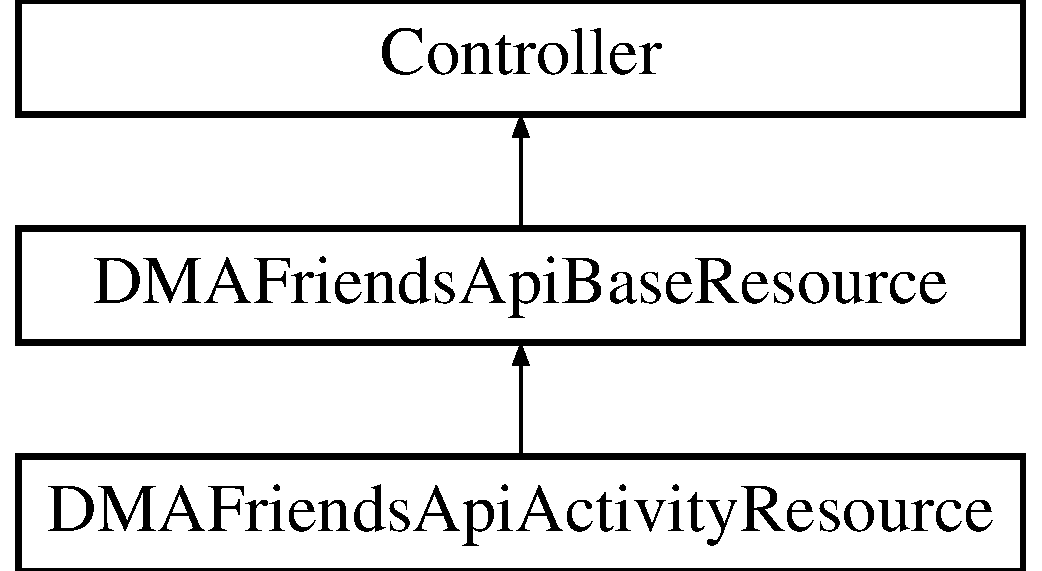
\includegraphics[height=3.000000cm]{d7/d53/classDMA_1_1Friends_1_1Api_1_1ActivityResource}
\end{center}
\end{figure}
\subsection*{Protected Attributes}
\begin{DoxyCompactItemize}
\item 
\hypertarget{classDMA_1_1Friends_1_1Api_1_1ActivityResource_a242d36374707954a784f08931e1796d9}{{\bfseries \$model} = '\textbackslash{}\hyperlink{classDMA_1_1Friends_1_1Models_1_1Activity}{D\+M\+A\textbackslash{}\+Friends\textbackslash{}\+Models\textbackslash{}\+Activity}'}\label{classDMA_1_1Friends_1_1Api_1_1ActivityResource_a242d36374707954a784f08931e1796d9}

\item 
\hypertarget{classDMA_1_1Friends_1_1Api_1_1ActivityResource_ab46a991a9e3980e6864c2c98c4fefe3a}{{\bfseries \$transformer} = '\textbackslash{}\hyperlink{classDMA_1_1Friends_1_1Api_1_1ActivityTransformer}{D\+M\+A\textbackslash{}\+Friends\textbackslash{}\+Api\textbackslash{}\+Activity\+Transformer}'}\label{classDMA_1_1Friends_1_1Api_1_1ActivityResource_ab46a991a9e3980e6864c2c98c4fefe3a}

\end{DoxyCompactItemize}
\subsection*{Additional Inherited Members}


The documentation for this class was generated from the following file\+:\begin{DoxyCompactItemize}
\item 
api/Activity\+Resource.\+php\end{DoxyCompactItemize}

\hypertarget{classDMA_1_1Friends_1_1Api_1_1ActivityTransformer}{\section{D\-M\-A\textbackslash{}Friends\textbackslash{}Api\textbackslash{}Activity\-Transformer Class Reference}
\label{classDMA_1_1Friends_1_1Api_1_1ActivityTransformer}\index{D\-M\-A\textbackslash{}\-Friends\textbackslash{}\-Api\textbackslash{}\-Activity\-Transformer@{D\-M\-A\textbackslash{}\-Friends\textbackslash{}\-Api\textbackslash{}\-Activity\-Transformer}}
}
Inheritance diagram for D\-M\-A\textbackslash{}Friends\textbackslash{}Api\textbackslash{}Activity\-Transformer\-:\begin{figure}[H]
\begin{center}
\leavevmode
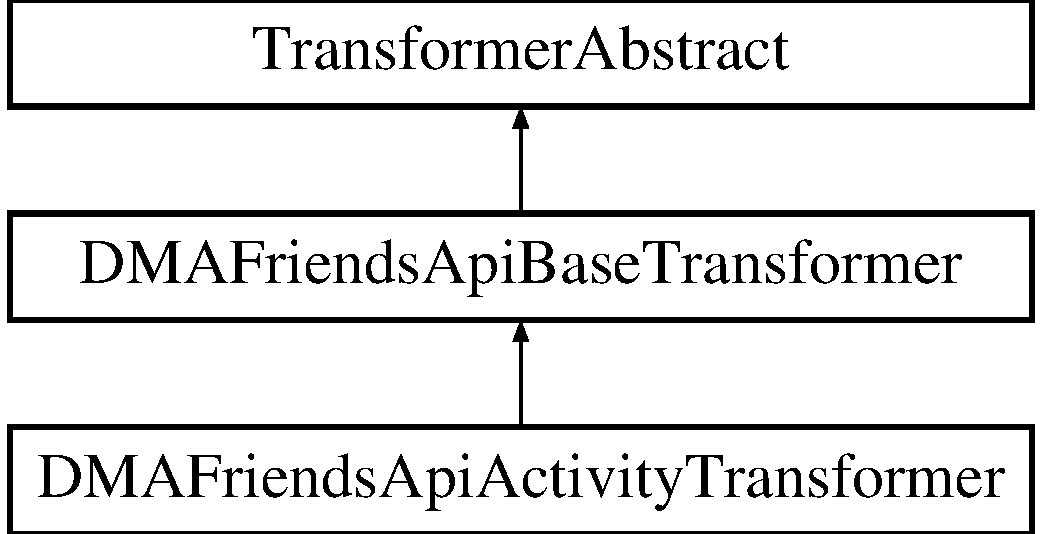
\includegraphics[height=3.000000cm]{d8/d07/classDMA_1_1Friends_1_1Api_1_1ActivityTransformer}
\end{center}
\end{figure}
\subsection*{Public Member Functions}
\begin{DoxyCompactItemize}
\item 
\hypertarget{classDMA_1_1Friends_1_1Api_1_1ActivityTransformer_a7d5e972a572a1448f4d230124d0d747e}{{\bfseries transforms} (Model \$instance)}\label{classDMA_1_1Friends_1_1Api_1_1ActivityTransformer_a7d5e972a572a1448f4d230124d0d747e}

\item 
\hyperlink{classDMA_1_1Friends_1_1Api_1_1ActivityTransformer_ad840be788d75759d0c2eb9874acb9b4a}{include\-Steps} (Model \$instance)
\end{DoxyCompactItemize}
\subsection*{Protected Attributes}
\begin{DoxyCompactItemize}
\item 
{\bfseries \$available\-Includes}
\end{DoxyCompactItemize}


\subsection{Member Function Documentation}
\hypertarget{classDMA_1_1Friends_1_1Api_1_1ActivityTransformer_ad840be788d75759d0c2eb9874acb9b4a}{\index{D\-M\-A\-::\-Friends\-::\-Api\-::\-Activity\-Transformer@{D\-M\-A\-::\-Friends\-::\-Api\-::\-Activity\-Transformer}!include\-Steps@{include\-Steps}}
\index{include\-Steps@{include\-Steps}!DMA::Friends::Api::ActivityTransformer@{D\-M\-A\-::\-Friends\-::\-Api\-::\-Activity\-Transformer}}
\subsubsection[{include\-Steps}]{\setlength{\rightskip}{0pt plus 5cm}D\-M\-A\textbackslash{}\-Friends\textbackslash{}\-Api\textbackslash{}\-Activity\-Transformer\-::include\-Steps (
\begin{DoxyParamCaption}
\item[{Model}]{\$instance}
\end{DoxyParamCaption}
)}}\label{classDMA_1_1Friends_1_1Api_1_1ActivityTransformer_ad840be788d75759d0c2eb9874acb9b4a}
Include Author

\begin{DoxyReturn}{Returns}
League 
\end{DoxyReturn}

\begin{DoxyCode}
39     \{
40         $stpes = $instance->steps;
41     
42         \textcolor{keywordflow}{return} $this->item($author, \textcolor{keyword}{new} StepResource);
43     \}    
\end{DoxyCode}


\subsection{Member Data Documentation}
\hypertarget{classDMA_1_1Friends_1_1Api_1_1ActivityTransformer_ab8cf362d22b93023b8f810dde08a4bc3}{\index{D\-M\-A\-::\-Friends\-::\-Api\-::\-Activity\-Transformer@{D\-M\-A\-::\-Friends\-::\-Api\-::\-Activity\-Transformer}!\$available\-Includes@{\$available\-Includes}}
\index{\$available\-Includes@{\$available\-Includes}!DMA::Friends::Api::ActivityTransformer@{D\-M\-A\-::\-Friends\-::\-Api\-::\-Activity\-Transformer}}
\subsubsection[{\$available\-Includes}]{\setlength{\rightskip}{0pt plus 5cm}D\-M\-A\textbackslash{}\-Friends\textbackslash{}\-Api\textbackslash{}\-Activity\-Transformer\-::\$available\-Includes\hspace{0.3cm}{\ttfamily [protected]}}}\label{classDMA_1_1Friends_1_1Api_1_1ActivityTransformer_ab8cf362d22b93023b8f810dde08a4bc3}
{\bfseries Initial value\-:}
\begin{DoxyCode}
= [
        \textcolor{stringliteral}{'steps'}
    ]
\end{DoxyCode}


The documentation for this class was generated from the following file\-:\begin{DoxyCompactItemize}
\item 
api/Activity\-Resource.\-php\end{DoxyCompactItemize}

\hypertarget{classDMA_1_1Friends_1_1Api_1_1ActivityTriggerResource}{\section{D\-M\-A\textbackslash{}Friends\textbackslash{}Api\textbackslash{}Activity\-Trigger\-Resource Class Reference}
\label{classDMA_1_1Friends_1_1Api_1_1ActivityTriggerResource}\index{D\-M\-A\textbackslash{}\-Friends\textbackslash{}\-Api\textbackslash{}\-Activity\-Trigger\-Resource@{D\-M\-A\textbackslash{}\-Friends\textbackslash{}\-Api\textbackslash{}\-Activity\-Trigger\-Resource}}
}
Inheritance diagram for D\-M\-A\textbackslash{}Friends\textbackslash{}Api\textbackslash{}Activity\-Trigger\-Resource\-:\begin{figure}[H]
\begin{center}
\leavevmode
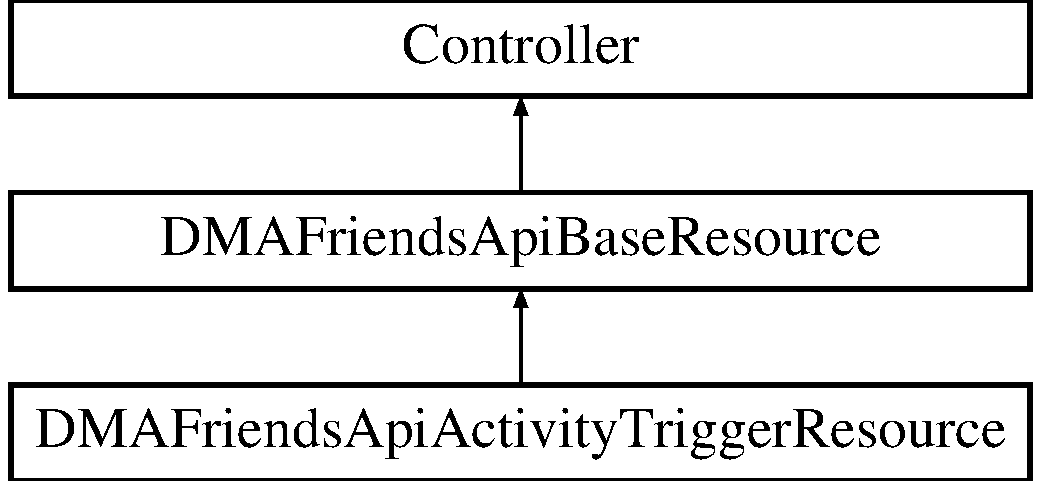
\includegraphics[height=3.000000cm]{dc/d89/classDMA_1_1Friends_1_1Api_1_1ActivityTriggerResource}
\end{center}
\end{figure}
\subsection*{Protected Attributes}
\begin{DoxyCompactItemize}
\item 
\hypertarget{classDMA_1_1Friends_1_1Api_1_1ActivityTriggerResource_ada7f5693b6e5dc676fe24187b48a4e7a}{{\bfseries \$model} = '\textbackslash{}\hyperlink{classDMA_1_1Friends_1_1Models_1_1ActivityTriggerType}{D\-M\-A\textbackslash{}\-Friends\textbackslash{}\-Models\textbackslash{}\-Activity\-Trigger\-Type}'}\label{classDMA_1_1Friends_1_1Api_1_1ActivityTriggerResource_ada7f5693b6e5dc676fe24187b48a4e7a}

\end{DoxyCompactItemize}
\subsection*{Additional Inherited Members}


The documentation for this class was generated from the following file\-:\begin{DoxyCompactItemize}
\item 
api/Activity\-Trigger\-Resource.\-php\end{DoxyCompactItemize}

\hypertarget{classDMA_1_1Friends_1_1Api_1_1ActivityTriggerTransformer}{\section{D\-M\-A\textbackslash{}Friends\textbackslash{}Api\textbackslash{}Activity\-Trigger\-Transformer Class Reference}
\label{classDMA_1_1Friends_1_1Api_1_1ActivityTriggerTransformer}\index{D\-M\-A\textbackslash{}\-Friends\textbackslash{}\-Api\textbackslash{}\-Activity\-Trigger\-Transformer@{D\-M\-A\textbackslash{}\-Friends\textbackslash{}\-Api\textbackslash{}\-Activity\-Trigger\-Transformer}}
}
Inheritance diagram for D\-M\-A\textbackslash{}Friends\textbackslash{}Api\textbackslash{}Activity\-Trigger\-Transformer\-:\begin{figure}[H]
\begin{center}
\leavevmode
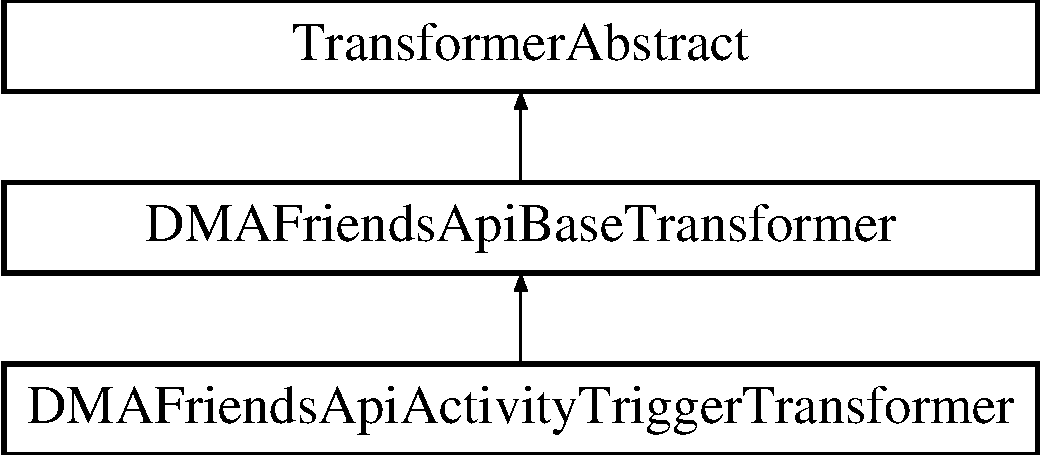
\includegraphics[height=3.000000cm]{df/dd0/classDMA_1_1Friends_1_1Api_1_1ActivityTriggerTransformer}
\end{center}
\end{figure}
\subsection*{Additional Inherited Members}


The documentation for this class was generated from the following file\-:\begin{DoxyCompactItemize}
\item 
api/Activity\-Trigger\-Resource.\-php\end{DoxyCompactItemize}

\hypertarget{classDMA_1_1Friends_1_1Models_1_1ActivityTriggerType}{\section{D\-M\-A\textbackslash{}Friends\textbackslash{}Models\textbackslash{}Activity\-Trigger\-Type Class Reference}
\label{classDMA_1_1Friends_1_1Models_1_1ActivityTriggerType}\index{D\-M\-A\textbackslash{}\-Friends\textbackslash{}\-Models\textbackslash{}\-Activity\-Trigger\-Type@{D\-M\-A\textbackslash{}\-Friends\textbackslash{}\-Models\textbackslash{}\-Activity\-Trigger\-Type}}
}
Inheritance diagram for D\-M\-A\textbackslash{}Friends\textbackslash{}Models\textbackslash{}Activity\-Trigger\-Type\-:\begin{figure}[H]
\begin{center}
\leavevmode
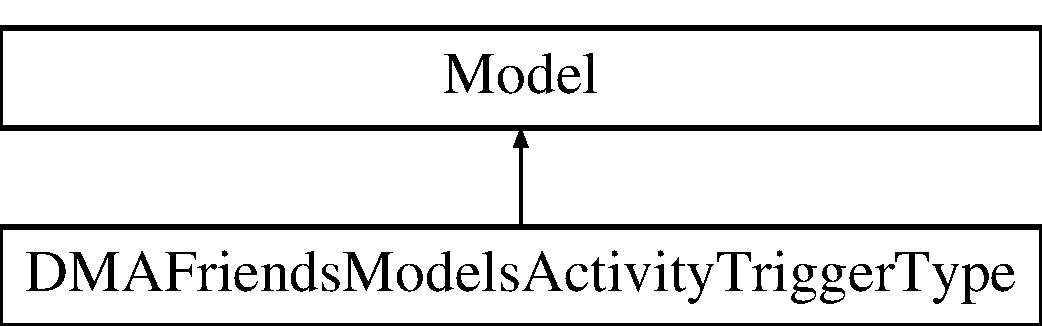
\includegraphics[height=2.000000cm]{d4/dc1/classDMA_1_1Friends_1_1Models_1_1ActivityTriggerType}
\end{center}
\end{figure}
\subsection*{Public Member Functions}
\begin{DoxyCompactItemize}
\item 
\hypertarget{classDMA_1_1Friends_1_1Models_1_1ActivityTriggerType_ad7d61fb031c7d4d9cf6a5b55bf555bec}{{\bfseries before\-Validate} ()}\label{classDMA_1_1Friends_1_1Models_1_1ActivityTriggerType_ad7d61fb031c7d4d9cf6a5b55bf555bec}

\end{DoxyCompactItemize}
\subsection*{Public Attributes}
\begin{DoxyCompactItemize}
\item 
\hypertarget{classDMA_1_1Friends_1_1Models_1_1ActivityTriggerType_a1dfd767d241b180576255684b4a09b32}{{\bfseries \$table} = 'dma\-\_\-friends\-\_\-activity\-\_\-trigger\-\_\-types'}\label{classDMA_1_1Friends_1_1Models_1_1ActivityTriggerType_a1dfd767d241b180576255684b4a09b32}

\item 
\hypertarget{classDMA_1_1Friends_1_1Models_1_1ActivityTriggerType_a6d228ad02fb8e2a94319a6b45e36f7fd}{{\bfseries \$timestamps} = false}\label{classDMA_1_1Friends_1_1Models_1_1ActivityTriggerType_a6d228ad02fb8e2a94319a6b45e36f7fd}

\item 
{\bfseries \$rules}
\item 
{\bfseries \$has\-Many}
\end{DoxyCompactItemize}
\subsection*{Protected Attributes}
\begin{DoxyCompactItemize}
\item 
\hypertarget{classDMA_1_1Friends_1_1Models_1_1ActivityTriggerType_ae1a545d11aac2fccd87fab15f3bc1d25}{{\bfseries \$guarded} = \mbox{[}'$\ast$'\mbox{]}}\label{classDMA_1_1Friends_1_1Models_1_1ActivityTriggerType_ae1a545d11aac2fccd87fab15f3bc1d25}

\item 
\hypertarget{classDMA_1_1Friends_1_1Models_1_1ActivityTriggerType_a17079823cdd50a41abe50ea541c4438b}{{\bfseries \$fillable} = \mbox{[}'touch'\mbox{]}}\label{classDMA_1_1Friends_1_1Models_1_1ActivityTriggerType_a17079823cdd50a41abe50ea541c4438b}

\end{DoxyCompactItemize}


\subsection{Detailed Description}
\hyperlink{classDMA_1_1Friends_1_1Models_1_1ActivityTriggerType}{Activity\-Trigger\-Type} Model 

\subsection{Member Data Documentation}
\hypertarget{classDMA_1_1Friends_1_1Models_1_1ActivityTriggerType_a044c92db10c394ad4d31f4383e277769}{\index{D\-M\-A\-::\-Friends\-::\-Models\-::\-Activity\-Trigger\-Type@{D\-M\-A\-::\-Friends\-::\-Models\-::\-Activity\-Trigger\-Type}!\$has\-Many@{\$has\-Many}}
\index{\$has\-Many@{\$has\-Many}!DMA::Friends::Models::ActivityTriggerType@{D\-M\-A\-::\-Friends\-::\-Models\-::\-Activity\-Trigger\-Type}}
\subsubsection[{\$has\-Many}]{\setlength{\rightskip}{0pt plus 5cm}D\-M\-A\textbackslash{}\-Friends\textbackslash{}\-Models\textbackslash{}\-Activity\-Trigger\-Type\-::\$has\-Many}}\label{classDMA_1_1Friends_1_1Models_1_1ActivityTriggerType_a044c92db10c394ad4d31f4383e277769}
{\bfseries Initial value\-:}
\begin{DoxyCode}
= [
        \textcolor{stringliteral}{'activities'} => [\textcolor{stringliteral}{'DMA\(\backslash\)Friends\(\backslash\)Models\(\backslash\)Activity'}, \textcolor{stringliteral}{'table'} => \textcolor{stringliteral}{'
      dma\_friends\_activity\_activity\_trigger\_type'}],
    ]
\end{DoxyCode}
\hypertarget{classDMA_1_1Friends_1_1Models_1_1ActivityTriggerType_ad12f065142d4b07860d55f2a028b17d9}{\index{D\-M\-A\-::\-Friends\-::\-Models\-::\-Activity\-Trigger\-Type@{D\-M\-A\-::\-Friends\-::\-Models\-::\-Activity\-Trigger\-Type}!\$rules@{\$rules}}
\index{\$rules@{\$rules}!DMA::Friends::Models::ActivityTriggerType@{D\-M\-A\-::\-Friends\-::\-Models\-::\-Activity\-Trigger\-Type}}
\subsubsection[{\$rules}]{\setlength{\rightskip}{0pt plus 5cm}D\-M\-A\textbackslash{}\-Friends\textbackslash{}\-Models\textbackslash{}\-Activity\-Trigger\-Type\-::\$rules}}\label{classDMA_1_1Friends_1_1Models_1_1ActivityTriggerType_ad12f065142d4b07860d55f2a028b17d9}
{\bfseries Initial value\-:}
\begin{DoxyCode}
= [ 
        \textcolor{stringliteral}{'name'} => \textcolor{stringliteral}{'required'}
\end{DoxyCode}


The documentation for this class was generated from the following file\-:\begin{DoxyCompactItemize}
\item 
models/Activity\-Trigger\-Type.\-php\end{DoxyCompactItemize}

\hypertarget{classDMA_1_1Friends_1_1Controllers_1_1ActivityTriggerTypes}{\section{D\-M\-A\textbackslash{}Friends\textbackslash{}Controllers\textbackslash{}Activity\-Trigger\-Types Class Reference}
\label{classDMA_1_1Friends_1_1Controllers_1_1ActivityTriggerTypes}\index{D\-M\-A\textbackslash{}\-Friends\textbackslash{}\-Controllers\textbackslash{}\-Activity\-Trigger\-Types@{D\-M\-A\textbackslash{}\-Friends\textbackslash{}\-Controllers\textbackslash{}\-Activity\-Trigger\-Types}}
}
Inheritance diagram for D\-M\-A\textbackslash{}Friends\textbackslash{}Controllers\textbackslash{}Activity\-Trigger\-Types\-:\begin{figure}[H]
\begin{center}
\leavevmode
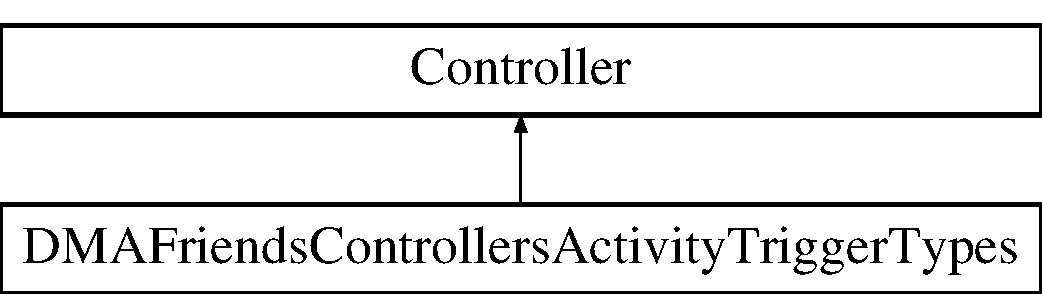
\includegraphics[height=2.000000cm]{d3/dbc/classDMA_1_1Friends_1_1Controllers_1_1ActivityTriggerTypes}
\end{center}
\end{figure}
\subsection*{Public Attributes}
\begin{DoxyCompactItemize}
\item 
{\bfseries \$implement}
\item 
\hypertarget{classDMA_1_1Friends_1_1Controllers_1_1ActivityTriggerTypes_add26deea49dcf3b76ef2dcae73249a34}{{\bfseries \$form\-Config} = 'config\-\_\-form.\-yaml'}\label{classDMA_1_1Friends_1_1Controllers_1_1ActivityTriggerTypes_add26deea49dcf3b76ef2dcae73249a34}

\item 
\hypertarget{classDMA_1_1Friends_1_1Controllers_1_1ActivityTriggerTypes_a4980b26c1a622da427205cdf840d9e43}{{\bfseries \$list\-Config} = 'config\-\_\-list.\-yaml'}\label{classDMA_1_1Friends_1_1Controllers_1_1ActivityTriggerTypes_a4980b26c1a622da427205cdf840d9e43}

\end{DoxyCompactItemize}


\subsection{Detailed Description}
\hyperlink{classDMA_1_1Friends_1_1Controllers_1_1ActivityTriggerTypes}{Activity\-Trigger\-Types} Back-\/end Controller 

\subsection{Member Data Documentation}
\hypertarget{classDMA_1_1Friends_1_1Controllers_1_1ActivityTriggerTypes_a7504906f92e023eb641a59fc21e2e07b}{\index{D\-M\-A\-::\-Friends\-::\-Controllers\-::\-Activity\-Trigger\-Types@{D\-M\-A\-::\-Friends\-::\-Controllers\-::\-Activity\-Trigger\-Types}!\$implement@{\$implement}}
\index{\$implement@{\$implement}!DMA::Friends::Controllers::ActivityTriggerTypes@{D\-M\-A\-::\-Friends\-::\-Controllers\-::\-Activity\-Trigger\-Types}}
\subsubsection[{\$implement}]{\setlength{\rightskip}{0pt plus 5cm}D\-M\-A\textbackslash{}\-Friends\textbackslash{}\-Controllers\textbackslash{}\-Activity\-Trigger\-Types\-::\$implement}}\label{classDMA_1_1Friends_1_1Controllers_1_1ActivityTriggerTypes_a7504906f92e023eb641a59fc21e2e07b}
{\bfseries Initial value\-:}
\begin{DoxyCode}
= [
        \textcolor{stringliteral}{'Backend.Behaviors.FormController'},
        \textcolor{stringliteral}{'Backend.Behaviors.ListController'}
    ]
\end{DoxyCode}


The documentation for this class was generated from the following file\-:\begin{DoxyCompactItemize}
\item 
controllers/Activity\-Trigger\-Types.\-php\end{DoxyCompactItemize}

\hypertarget{classDMA_1_1Friends_1_1Models_1_1ActivityType}{\section{D\-M\-A\textbackslash{}Friends\textbackslash{}Models\textbackslash{}Activity\-Type Class Reference}
\label{classDMA_1_1Friends_1_1Models_1_1ActivityType}\index{D\-M\-A\textbackslash{}\-Friends\textbackslash{}\-Models\textbackslash{}\-Activity\-Type@{D\-M\-A\textbackslash{}\-Friends\textbackslash{}\-Models\textbackslash{}\-Activity\-Type}}
}
Inheritance diagram for D\-M\-A\textbackslash{}Friends\textbackslash{}Models\textbackslash{}Activity\-Type\-:\begin{figure}[H]
\begin{center}
\leavevmode
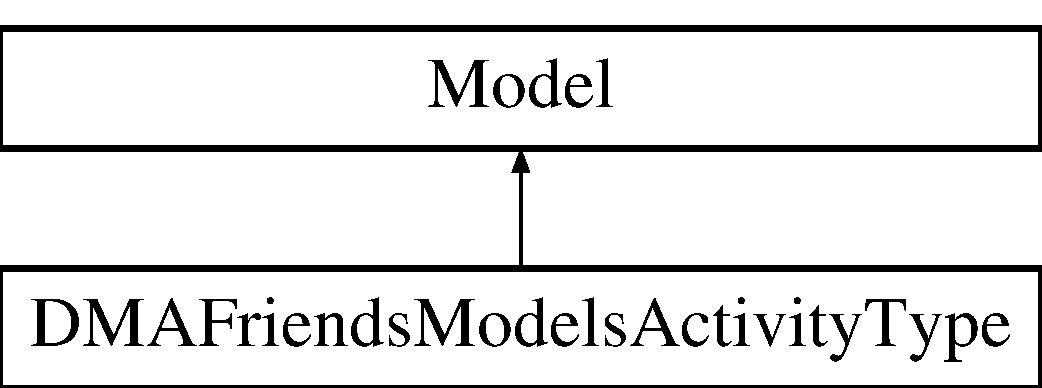
\includegraphics[height=2.000000cm]{d6/d9b/classDMA_1_1Friends_1_1Models_1_1ActivityType}
\end{center}
\end{figure}
\subsection*{Public Member Functions}
\begin{DoxyCompactItemize}
\item 
\hypertarget{classDMA_1_1Friends_1_1Models_1_1ActivityType_a83d0835e12b070150ef95a37a4c2ca03}{{\bfseries before\-Validate} ()}\label{classDMA_1_1Friends_1_1Models_1_1ActivityType_a83d0835e12b070150ef95a37a4c2ca03}

\end{DoxyCompactItemize}
\subsection*{Public Attributes}
\begin{DoxyCompactItemize}
\item 
\hypertarget{classDMA_1_1Friends_1_1Models_1_1ActivityType_a439a95f54467ed98c4db4e130c37b733}{{\bfseries \$table} = 'dma\-\_\-friends\-\_\-activity\-\_\-types'}\label{classDMA_1_1Friends_1_1Models_1_1ActivityType_a439a95f54467ed98c4db4e130c37b733}

\item 
\hypertarget{classDMA_1_1Friends_1_1Models_1_1ActivityType_acf0a62230181f0a541aba2e335df5db7}{{\bfseries \$timestamps} = false}\label{classDMA_1_1Friends_1_1Models_1_1ActivityType_acf0a62230181f0a541aba2e335df5db7}

\item 
{\bfseries \$rules}
\item 
{\bfseries \$has\-Many}
\end{DoxyCompactItemize}
\subsection*{Protected Attributes}
\begin{DoxyCompactItemize}
\item 
\hypertarget{classDMA_1_1Friends_1_1Models_1_1ActivityType_a8168d7847a4167cf499bf8c95a3fdb17}{{\bfseries \$guarded} = \mbox{[}'$\ast$'\mbox{]}}\label{classDMA_1_1Friends_1_1Models_1_1ActivityType_a8168d7847a4167cf499bf8c95a3fdb17}

\item 
\hypertarget{classDMA_1_1Friends_1_1Models_1_1ActivityType_ac98dbccc38d9f41ab37fb367238a1396}{{\bfseries \$fillable} = \mbox{[}$\,$\mbox{]}}\label{classDMA_1_1Friends_1_1Models_1_1ActivityType_ac98dbccc38d9f41ab37fb367238a1396}

\end{DoxyCompactItemize}


\subsection{Detailed Description}
\hyperlink{classDMA_1_1Friends_1_1Models_1_1ActivityType}{Activity\-Type} Model 

\subsection{Member Data Documentation}
\hypertarget{classDMA_1_1Friends_1_1Models_1_1ActivityType_ab2f9dcb8f38fe05674e0ca65ef86c061}{\index{D\-M\-A\-::\-Friends\-::\-Models\-::\-Activity\-Type@{D\-M\-A\-::\-Friends\-::\-Models\-::\-Activity\-Type}!\$has\-Many@{\$has\-Many}}
\index{\$has\-Many@{\$has\-Many}!DMA::Friends::Models::ActivityType@{D\-M\-A\-::\-Friends\-::\-Models\-::\-Activity\-Type}}
\subsubsection[{\$has\-Many}]{\setlength{\rightskip}{0pt plus 5cm}D\-M\-A\textbackslash{}\-Friends\textbackslash{}\-Models\textbackslash{}\-Activity\-Type\-::\$has\-Many}}\label{classDMA_1_1Friends_1_1Models_1_1ActivityType_ab2f9dcb8f38fe05674e0ca65ef86c061}
{\bfseries Initial value\-:}
\begin{DoxyCode}
= [
        \textcolor{stringliteral}{'activities'}    => [\textcolor{stringliteral}{'DMA\(\backslash\)Friends\(\backslash\)Models\(\backslash\)Activity'}]
\end{DoxyCode}
\hypertarget{classDMA_1_1Friends_1_1Models_1_1ActivityType_a15a6ae9c0d6533dfd440a14afce6691c}{\index{D\-M\-A\-::\-Friends\-::\-Models\-::\-Activity\-Type@{D\-M\-A\-::\-Friends\-::\-Models\-::\-Activity\-Type}!\$rules@{\$rules}}
\index{\$rules@{\$rules}!DMA::Friends::Models::ActivityType@{D\-M\-A\-::\-Friends\-::\-Models\-::\-Activity\-Type}}
\subsubsection[{\$rules}]{\setlength{\rightskip}{0pt plus 5cm}D\-M\-A\textbackslash{}\-Friends\textbackslash{}\-Models\textbackslash{}\-Activity\-Type\-::\$rules}}\label{classDMA_1_1Friends_1_1Models_1_1ActivityType_a15a6ae9c0d6533dfd440a14afce6691c}
{\bfseries Initial value\-:}
\begin{DoxyCode}
= [ 
        \textcolor{stringliteral}{'name'} => \textcolor{stringliteral}{'required'}
\end{DoxyCode}


The documentation for this class was generated from the following file\-:\begin{DoxyCompactItemize}
\item 
models/Activity\-Type.\-php\end{DoxyCompactItemize}

\hypertarget{classDMA_1_1Friends_1_1Api_1_1ActivityTypeResource}{\section{D\-M\-A\textbackslash{}Friends\textbackslash{}Api\textbackslash{}Activity\-Type\-Resource Class Reference}
\label{classDMA_1_1Friends_1_1Api_1_1ActivityTypeResource}\index{D\-M\-A\textbackslash{}\-Friends\textbackslash{}\-Api\textbackslash{}\-Activity\-Type\-Resource@{D\-M\-A\textbackslash{}\-Friends\textbackslash{}\-Api\textbackslash{}\-Activity\-Type\-Resource}}
}
Inheritance diagram for D\-M\-A\textbackslash{}Friends\textbackslash{}Api\textbackslash{}Activity\-Type\-Resource\-:\begin{figure}[H]
\begin{center}
\leavevmode
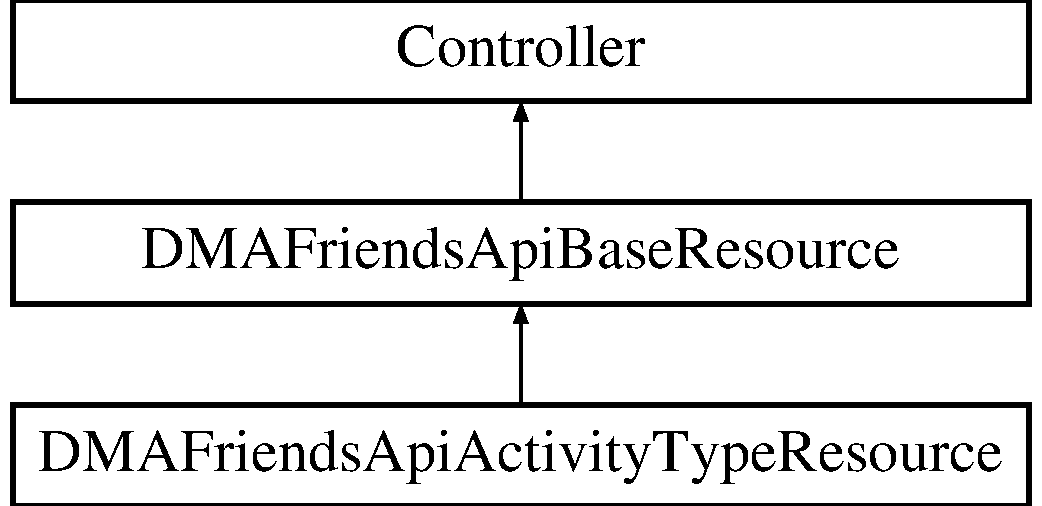
\includegraphics[height=3.000000cm]{d4/d36/classDMA_1_1Friends_1_1Api_1_1ActivityTypeResource}
\end{center}
\end{figure}
\subsection*{Protected Attributes}
\begin{DoxyCompactItemize}
\item 
\hypertarget{classDMA_1_1Friends_1_1Api_1_1ActivityTypeResource_adbfb8930be9081353d18b93174a97797}{{\bfseries \$model} = '\textbackslash{}\hyperlink{classDMA_1_1Friends_1_1Models_1_1ActivityType}{D\-M\-A\textbackslash{}\-Friends\textbackslash{}\-Models\textbackslash{}\-Activity\-Type}'}\label{classDMA_1_1Friends_1_1Api_1_1ActivityTypeResource_adbfb8930be9081353d18b93174a97797}

\end{DoxyCompactItemize}
\subsection*{Additional Inherited Members}


The documentation for this class was generated from the following file\-:\begin{DoxyCompactItemize}
\item 
api/Activity\-Type\-Resource.\-php\end{DoxyCompactItemize}

\hypertarget{classDMA_1_1Friends_1_1Controllers_1_1ActivityTypes}{\section{D\-M\-A\textbackslash{}Friends\textbackslash{}Controllers\textbackslash{}Activity\-Types Class Reference}
\label{classDMA_1_1Friends_1_1Controllers_1_1ActivityTypes}\index{D\-M\-A\textbackslash{}\-Friends\textbackslash{}\-Controllers\textbackslash{}\-Activity\-Types@{D\-M\-A\textbackslash{}\-Friends\textbackslash{}\-Controllers\textbackslash{}\-Activity\-Types}}
}
Inheritance diagram for D\-M\-A\textbackslash{}Friends\textbackslash{}Controllers\textbackslash{}Activity\-Types\-:\begin{figure}[H]
\begin{center}
\leavevmode
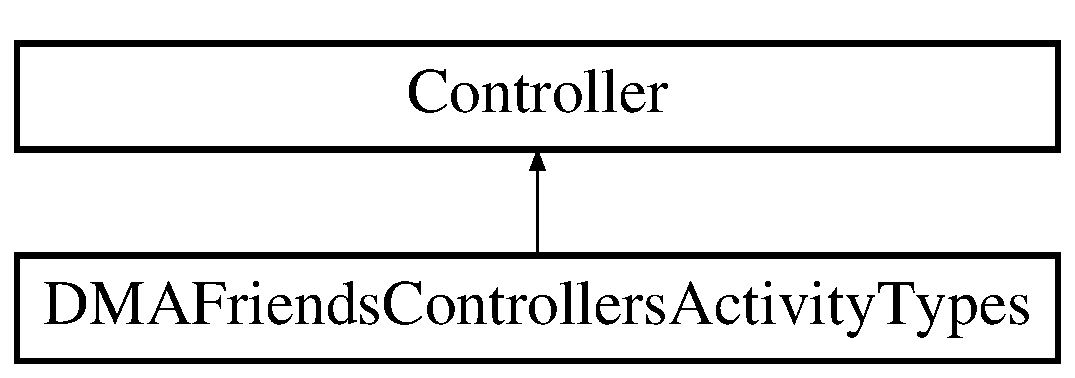
\includegraphics[height=2.000000cm]{d6/d9d/classDMA_1_1Friends_1_1Controllers_1_1ActivityTypes}
\end{center}
\end{figure}
\subsection*{Public Attributes}
\begin{DoxyCompactItemize}
\item 
{\bfseries \$implement}
\item 
\hypertarget{classDMA_1_1Friends_1_1Controllers_1_1ActivityTypes_abf63526872073fe5db2ab8b6360b03e4}{{\bfseries \$form\-Config} = 'config\-\_\-form.\-yaml'}\label{classDMA_1_1Friends_1_1Controllers_1_1ActivityTypes_abf63526872073fe5db2ab8b6360b03e4}

\item 
\hypertarget{classDMA_1_1Friends_1_1Controllers_1_1ActivityTypes_a104d438fcc651182015d73628605eb4b}{{\bfseries \$list\-Config} = 'config\-\_\-list.\-yaml'}\label{classDMA_1_1Friends_1_1Controllers_1_1ActivityTypes_a104d438fcc651182015d73628605eb4b}

\end{DoxyCompactItemize}


\subsection{Detailed Description}
\hyperlink{classDMA_1_1Friends_1_1Controllers_1_1ActivityTypes}{Activity\-Types} Back-\/end Controller 

\subsection{Member Data Documentation}
\hypertarget{classDMA_1_1Friends_1_1Controllers_1_1ActivityTypes_a8056141ce368e3e68051b75f6d785730}{\index{D\-M\-A\-::\-Friends\-::\-Controllers\-::\-Activity\-Types@{D\-M\-A\-::\-Friends\-::\-Controllers\-::\-Activity\-Types}!\$implement@{\$implement}}
\index{\$implement@{\$implement}!DMA::Friends::Controllers::ActivityTypes@{D\-M\-A\-::\-Friends\-::\-Controllers\-::\-Activity\-Types}}
\subsubsection[{\$implement}]{\setlength{\rightskip}{0pt plus 5cm}D\-M\-A\textbackslash{}\-Friends\textbackslash{}\-Controllers\textbackslash{}\-Activity\-Types\-::\$implement}}\label{classDMA_1_1Friends_1_1Controllers_1_1ActivityTypes_a8056141ce368e3e68051b75f6d785730}
{\bfseries Initial value\-:}
\begin{DoxyCode}
= [
        \textcolor{stringliteral}{'Backend.Behaviors.FormController'},
        \textcolor{stringliteral}{'Backend.Behaviors.ListController'}
    ]
\end{DoxyCode}


The documentation for this class was generated from the following file\-:\begin{DoxyCompactItemize}
\item 
controllers/Activity\-Types.\-php\end{DoxyCompactItemize}

\hypertarget{classDMA_1_1Friends_1_1Api_1_1ActivityTypeTransformer}{\section{D\-M\-A\textbackslash{}Friends\textbackslash{}Api\textbackslash{}Activity\-Type\-Transformer Class Reference}
\label{classDMA_1_1Friends_1_1Api_1_1ActivityTypeTransformer}\index{D\-M\-A\textbackslash{}\-Friends\textbackslash{}\-Api\textbackslash{}\-Activity\-Type\-Transformer@{D\-M\-A\textbackslash{}\-Friends\textbackslash{}\-Api\textbackslash{}\-Activity\-Type\-Transformer}}
}
Inheritance diagram for D\-M\-A\textbackslash{}Friends\textbackslash{}Api\textbackslash{}Activity\-Type\-Transformer\-:\begin{figure}[H]
\begin{center}
\leavevmode
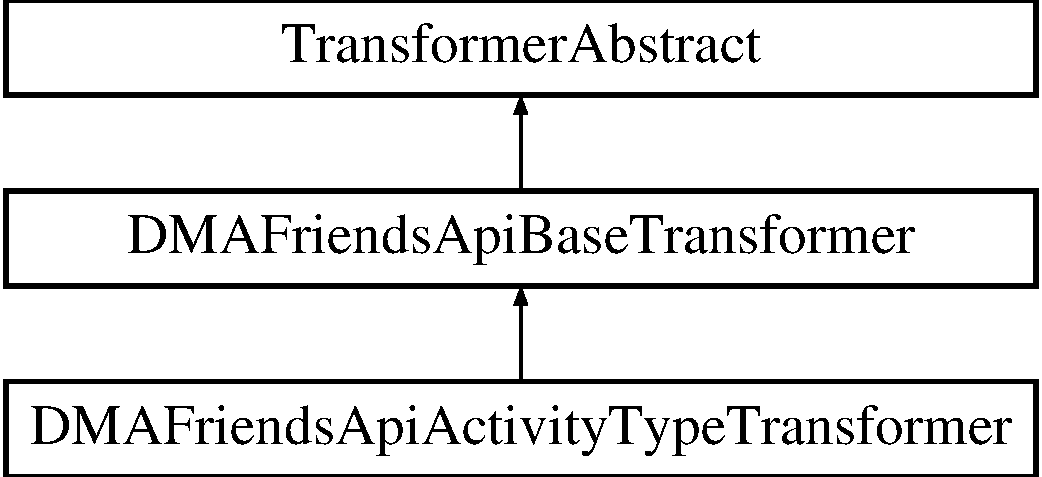
\includegraphics[height=3.000000cm]{d2/dfa/classDMA_1_1Friends_1_1Api_1_1ActivityTypeTransformer}
\end{center}
\end{figure}
\subsection*{Additional Inherited Members}


The documentation for this class was generated from the following file\-:\begin{DoxyCompactItemize}
\item 
api/Activity\-Type\-Resource.\-php\end{DoxyCompactItemize}

\hypertarget{classDMA_1_1Friends_1_1Models_1_1Badge}{\section{D\+M\+A\textbackslash{}Friends\textbackslash{}Models\textbackslash{}Badge Class Reference}
\label{classDMA_1_1Friends_1_1Models_1_1Badge}\index{D\+M\+A\textbackslash{}\+Friends\textbackslash{}\+Models\textbackslash{}\+Badge@{D\+M\+A\textbackslash{}\+Friends\textbackslash{}\+Models\textbackslash{}\+Badge}}
}
Inheritance diagram for D\+M\+A\textbackslash{}Friends\textbackslash{}Models\textbackslash{}Badge\+:\begin{figure}[H]
\begin{center}
\leavevmode
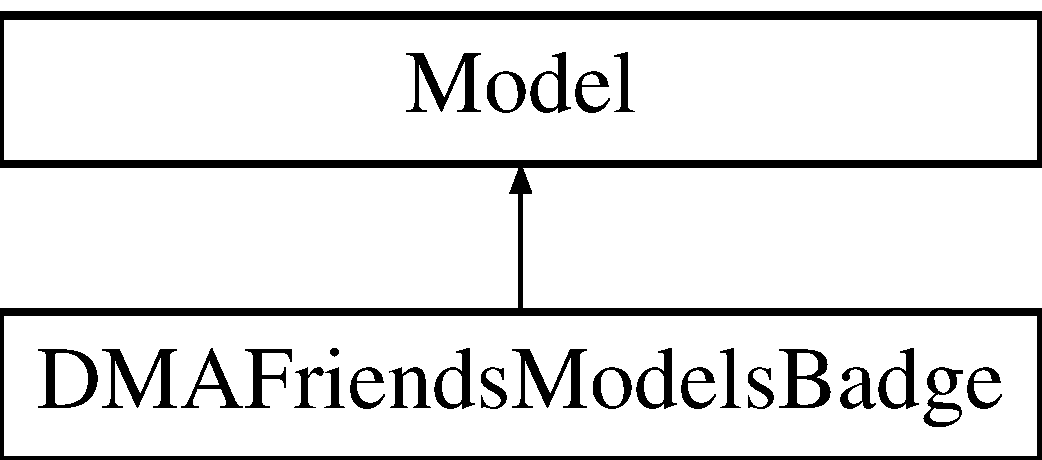
\includegraphics[height=2.000000cm]{df/d98/classDMA_1_1Friends_1_1Models_1_1Badge}
\end{center}
\end{figure}
\subsection*{Public Member Functions}
\begin{DoxyCompactItemize}
\item 
\hypertarget{classDMA_1_1Friends_1_1Models_1_1Badge_a65fc600bfefbedc8d7393ec86c848a51}{{\bfseries scope\+Not\+Completed} (\$query, User \$user)}\label{classDMA_1_1Friends_1_1Models_1_1Badge_a65fc600bfefbedc8d7393ec86c848a51}

\item 
\hypertarget{classDMA_1_1Friends_1_1Models_1_1Badge_a5ebdc91135362ca2b0225fdb0c965127}{{\bfseries scopefind\+Wordpress} (\$query, \$id)}\label{classDMA_1_1Friends_1_1Models_1_1Badge_a5ebdc91135362ca2b0225fdb0c965127}

\item 
\hypertarget{classDMA_1_1Friends_1_1Models_1_1Badge_ac40fb9fa1c7f70f29bb90e77b8f9c8aa}{{\bfseries steps} ()}\label{classDMA_1_1Friends_1_1Models_1_1Badge_ac40fb9fa1c7f70f29bb90e77b8f9c8aa}

\end{DoxyCompactItemize}
\subsection*{Public Attributes}
\begin{DoxyCompactItemize}
\item 
\hypertarget{classDMA_1_1Friends_1_1Models_1_1Badge_aa58560300753d15561b1a979aa21b8fd}{{\bfseries \$table} = 'dma\+\_\+friends\+\_\+badges'}\label{classDMA_1_1Friends_1_1Models_1_1Badge_aa58560300753d15561b1a979aa21b8fd}

\item 
{\bfseries \$rules}
\item 
{\bfseries \$has\+Many}
\item 
{\bfseries \$belongs\+To\+Many}
\item 
{\bfseries \$attach\+One}
\item 
{\bfseries \$morph\+Many}
\item 
{\bfseries \$morph\+To\+Many}
\end{DoxyCompactItemize}
\subsection*{Protected Attributes}
\begin{DoxyCompactItemize}
\item 
\hypertarget{classDMA_1_1Friends_1_1Models_1_1Badge_ae0b360f20ce06a26af28c91de3f63e11}{{\bfseries \$guarded} = \mbox{[}'$\ast$'\mbox{]}}\label{classDMA_1_1Friends_1_1Models_1_1Badge_ae0b360f20ce06a26af28c91de3f63e11}

\item 
\hypertarget{classDMA_1_1Friends_1_1Models_1_1Badge_a4d4f326e6071e6d44fdb54d93d579c44}{{\bfseries \$fillable} = \mbox{[}'touch'\mbox{]}}\label{classDMA_1_1Friends_1_1Models_1_1Badge_a4d4f326e6071e6d44fdb54d93d579c44}

\item 
\hypertarget{classDMA_1_1Friends_1_1Models_1_1Badge_ae8aa2206bbd9a6e152db7691a0dfd0b5}{{\bfseries \$dates} = \mbox{[}'date\+\_\+begin', 'date\+\_\+end'\mbox{]}}\label{classDMA_1_1Friends_1_1Models_1_1Badge_ae8aa2206bbd9a6e152db7691a0dfd0b5}

\end{DoxyCompactItemize}


\subsection{Detailed Description}
\hyperlink{classDMA_1_1Friends_1_1Models_1_1Badge}{Badge} Model 

\subsection{Member Data Documentation}
\hypertarget{classDMA_1_1Friends_1_1Models_1_1Badge_abd4795b249f74dd23651f51479fbe5fb}{\index{D\+M\+A\+::\+Friends\+::\+Models\+::\+Badge@{D\+M\+A\+::\+Friends\+::\+Models\+::\+Badge}!\$attach\+One@{\$attach\+One}}
\index{\$attach\+One@{\$attach\+One}!D\+M\+A\+::\+Friends\+::\+Models\+::\+Badge@{D\+M\+A\+::\+Friends\+::\+Models\+::\+Badge}}
\subsubsection[{\$attach\+One}]{\setlength{\rightskip}{0pt plus 5cm}D\+M\+A\textbackslash{}\+Friends\textbackslash{}\+Models\textbackslash{}\+Badge\+::\$attach\+One}}\label{classDMA_1_1Friends_1_1Models_1_1Badge_abd4795b249f74dd23651f51479fbe5fb}
{\bfseries Initial value\+:}
\begin{DoxyCode}
= [
        \textcolor{stringliteral}{'image'} => [\textcolor{stringliteral}{'System\(\backslash\)Models\(\backslash\)File'}]
    ]
\end{DoxyCode}
\hypertarget{classDMA_1_1Friends_1_1Models_1_1Badge_ab143958e8f63d5b612832fee145f0aa1}{\index{D\+M\+A\+::\+Friends\+::\+Models\+::\+Badge@{D\+M\+A\+::\+Friends\+::\+Models\+::\+Badge}!\$belongs\+To\+Many@{\$belongs\+To\+Many}}
\index{\$belongs\+To\+Many@{\$belongs\+To\+Many}!D\+M\+A\+::\+Friends\+::\+Models\+::\+Badge@{D\+M\+A\+::\+Friends\+::\+Models\+::\+Badge}}
\subsubsection[{\$belongs\+To\+Many}]{\setlength{\rightskip}{0pt plus 5cm}D\+M\+A\textbackslash{}\+Friends\textbackslash{}\+Models\textbackslash{}\+Badge\+::\$belongs\+To\+Many}}\label{classDMA_1_1Friends_1_1Models_1_1Badge_ab143958e8f63d5b612832fee145f0aa1}
{\bfseries Initial value\+:}
\begin{DoxyCode}
= [
        \textcolor{stringliteral}{'users'} => [\textcolor{stringliteral}{'RainLab\(\backslash\)User\(\backslash\)Models\(\backslash\)User'}, \textcolor{stringliteral}{'dma\_friends\_badge\_user'}]
\end{DoxyCode}
\hypertarget{classDMA_1_1Friends_1_1Models_1_1Badge_a1b363de2d8c44cd12dff6bca90a6b212}{\index{D\+M\+A\+::\+Friends\+::\+Models\+::\+Badge@{D\+M\+A\+::\+Friends\+::\+Models\+::\+Badge}!\$has\+Many@{\$has\+Many}}
\index{\$has\+Many@{\$has\+Many}!D\+M\+A\+::\+Friends\+::\+Models\+::\+Badge@{D\+M\+A\+::\+Friends\+::\+Models\+::\+Badge}}
\subsubsection[{\$has\+Many}]{\setlength{\rightskip}{0pt plus 5cm}D\+M\+A\textbackslash{}\+Friends\textbackslash{}\+Models\textbackslash{}\+Badge\+::\$has\+Many}}\label{classDMA_1_1Friends_1_1Models_1_1Badge_a1b363de2d8c44cd12dff6bca90a6b212}
{\bfseries Initial value\+:}
\begin{DoxyCode}
= [
        \textcolor{stringliteral}{'steps'} => [\textcolor{stringliteral}{'DMA\(\backslash\)Friends\(\backslash\)Models\(\backslash\)Step'}]
\end{DoxyCode}
\hypertarget{classDMA_1_1Friends_1_1Models_1_1Badge_a239fed984baad287f15badaaece428ff}{\index{D\+M\+A\+::\+Friends\+::\+Models\+::\+Badge@{D\+M\+A\+::\+Friends\+::\+Models\+::\+Badge}!\$morph\+Many@{\$morph\+Many}}
\index{\$morph\+Many@{\$morph\+Many}!D\+M\+A\+::\+Friends\+::\+Models\+::\+Badge@{D\+M\+A\+::\+Friends\+::\+Models\+::\+Badge}}
\subsubsection[{\$morph\+Many}]{\setlength{\rightskip}{0pt plus 5cm}D\+M\+A\textbackslash{}\+Friends\textbackslash{}\+Models\textbackslash{}\+Badge\+::\$morph\+Many}}\label{classDMA_1_1Friends_1_1Models_1_1Badge_a239fed984baad287f15badaaece428ff}
{\bfseries Initial value\+:}
\begin{DoxyCode}
= [
        \textcolor{stringliteral}{'activityLogs'}  => [\textcolor{stringliteral}{'DMA\(\backslash\)Friends\(\backslash\)Models\(\backslash\)ActivityLog'}, \textcolor{stringliteral}{'name'} => \textcolor{stringliteral}{'object'}],
    ]
\end{DoxyCode}
\hypertarget{classDMA_1_1Friends_1_1Models_1_1Badge_a2efb4ca933422dfb4ca416676d73cad0}{\index{D\+M\+A\+::\+Friends\+::\+Models\+::\+Badge@{D\+M\+A\+::\+Friends\+::\+Models\+::\+Badge}!\$morph\+To\+Many@{\$morph\+To\+Many}}
\index{\$morph\+To\+Many@{\$morph\+To\+Many}!D\+M\+A\+::\+Friends\+::\+Models\+::\+Badge@{D\+M\+A\+::\+Friends\+::\+Models\+::\+Badge}}
\subsubsection[{\$morph\+To\+Many}]{\setlength{\rightskip}{0pt plus 5cm}D\+M\+A\textbackslash{}\+Friends\textbackslash{}\+Models\textbackslash{}\+Badge\+::\$morph\+To\+Many}}\label{classDMA_1_1Friends_1_1Models_1_1Badge_a2efb4ca933422dfb4ca416676d73cad0}
{\bfseries Initial value\+:}
\begin{DoxyCode}
= [
        \textcolor{stringliteral}{'categories'}    => [\textcolor{stringliteral}{'DMA\(\backslash\)Friends\(\backslash\)Models\(\backslash\)Category'}, \textcolor{stringliteral}{'name'} => \textcolor{stringliteral}{'object'}
\end{DoxyCode}
\hypertarget{classDMA_1_1Friends_1_1Models_1_1Badge_ab750ee2c75af273ca930a12b1a20b3ae}{\index{D\+M\+A\+::\+Friends\+::\+Models\+::\+Badge@{D\+M\+A\+::\+Friends\+::\+Models\+::\+Badge}!\$rules@{\$rules}}
\index{\$rules@{\$rules}!D\+M\+A\+::\+Friends\+::\+Models\+::\+Badge@{D\+M\+A\+::\+Friends\+::\+Models\+::\+Badge}}
\subsubsection[{\$rules}]{\setlength{\rightskip}{0pt plus 5cm}D\+M\+A\textbackslash{}\+Friends\textbackslash{}\+Models\textbackslash{}\+Badge\+::\$rules}}\label{classDMA_1_1Friends_1_1Models_1_1Badge_ab750ee2c75af273ca930a12b1a20b3ae}
{\bfseries Initial value\+:}
\begin{DoxyCode}
= [ 
        \textcolor{stringliteral}{'title'} => \textcolor{stringliteral}{'required'}
\end{DoxyCode}


The documentation for this class was generated from the following file\+:\begin{DoxyCompactItemize}
\item 
models/Badge.\+php\end{DoxyCompactItemize}

\hypertarget{classDMA_1_1Friends_1_1Wordpress_1_1Badge}{}\section{D\+M\+A\textbackslash{}Friends\textbackslash{}Wordpress\textbackslash{}Badge Class Reference}
\label{classDMA_1_1Friends_1_1Wordpress_1_1Badge}\index{D\+M\+A\textbackslash{}\+Friends\textbackslash{}\+Wordpress\textbackslash{}\+Badge@{D\+M\+A\textbackslash{}\+Friends\textbackslash{}\+Wordpress\textbackslash{}\+Badge}}
Inheritance diagram for D\+M\+A\textbackslash{}Friends\textbackslash{}Wordpress\textbackslash{}Badge\+:\begin{figure}[H]
\begin{center}
\leavevmode
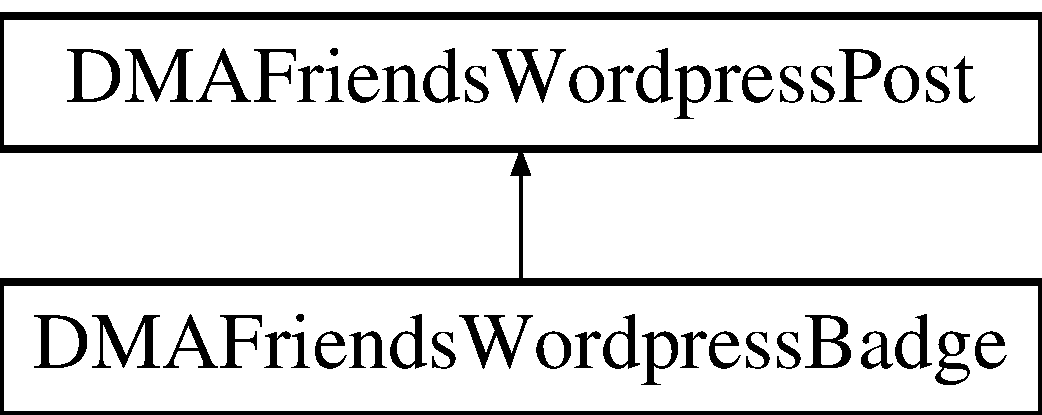
\includegraphics[height=2.000000cm]{d8/d3a/classDMA_1_1Friends_1_1Wordpress_1_1Badge}
\end{center}
\end{figure}
\subsection*{Public Attributes}
\begin{DoxyCompactItemize}
\item 
\hyperlink{classDMA_1_1Friends_1_1Wordpress_1_1Badge_a3044aa841b86f76868023889de4ca114}{\$post\+Type} = \textquotesingle{}badge\textquotesingle{}
\end{DoxyCompactItemize}
\subsection*{Additional Inherited Members}


\subsection{Member Data Documentation}
\hypertarget{classDMA_1_1Friends_1_1Wordpress_1_1Badge_a3044aa841b86f76868023889de4ca114}{}\index{D\+M\+A\+::\+Friends\+::\+Wordpress\+::\+Badge@{D\+M\+A\+::\+Friends\+::\+Wordpress\+::\+Badge}!\$post\+Type@{\$post\+Type}}
\index{\$post\+Type@{\$post\+Type}!D\+M\+A\+::\+Friends\+::\+Wordpress\+::\+Badge@{D\+M\+A\+::\+Friends\+::\+Wordpress\+::\+Badge}}
\subsubsection[{\$post\+Type}]{\setlength{\rightskip}{0pt plus 5cm}D\+M\+A\textbackslash{}\+Friends\textbackslash{}\+Wordpress\textbackslash{}\+Badge\+::\$post\+Type = \textquotesingle{}badge\textquotesingle{}}\label{classDMA_1_1Friends_1_1Wordpress_1_1Badge_a3044aa841b86f76868023889de4ca114}
Override default post type 

The documentation for this class was generated from the following file\+:\begin{DoxyCompactItemize}
\item 
wordpress/Badge.\+php\end{DoxyCompactItemize}

\hypertarget{classDMA_1_1Friends_1_1Classes_1_1BadgeProcessor}{\section{D\-M\-A\textbackslash{}Friends\textbackslash{}Classes\textbackslash{}Badge\-Processor Class Reference}
\label{classDMA_1_1Friends_1_1Classes_1_1BadgeProcessor}\index{D\-M\-A\textbackslash{}\-Friends\textbackslash{}\-Classes\textbackslash{}\-Badge\-Processor@{D\-M\-A\textbackslash{}\-Friends\textbackslash{}\-Classes\textbackslash{}\-Badge\-Processor}}
}


The documentation for this class was generated from the following file\-:\begin{DoxyCompactItemize}
\item 
classes/Badge\-Processor.\-php\end{DoxyCompactItemize}

\hypertarget{classDMA_1_1Friends_1_1Api_1_1BadgeResource}{\section{D\-M\-A\textbackslash{}Friends\textbackslash{}Api\textbackslash{}Badge\-Resource Class Reference}
\label{classDMA_1_1Friends_1_1Api_1_1BadgeResource}\index{D\-M\-A\textbackslash{}\-Friends\textbackslash{}\-Api\textbackslash{}\-Badge\-Resource@{D\-M\-A\textbackslash{}\-Friends\textbackslash{}\-Api\textbackslash{}\-Badge\-Resource}}
}
Inheritance diagram for D\-M\-A\textbackslash{}Friends\textbackslash{}Api\textbackslash{}Badge\-Resource\-:\begin{figure}[H]
\begin{center}
\leavevmode
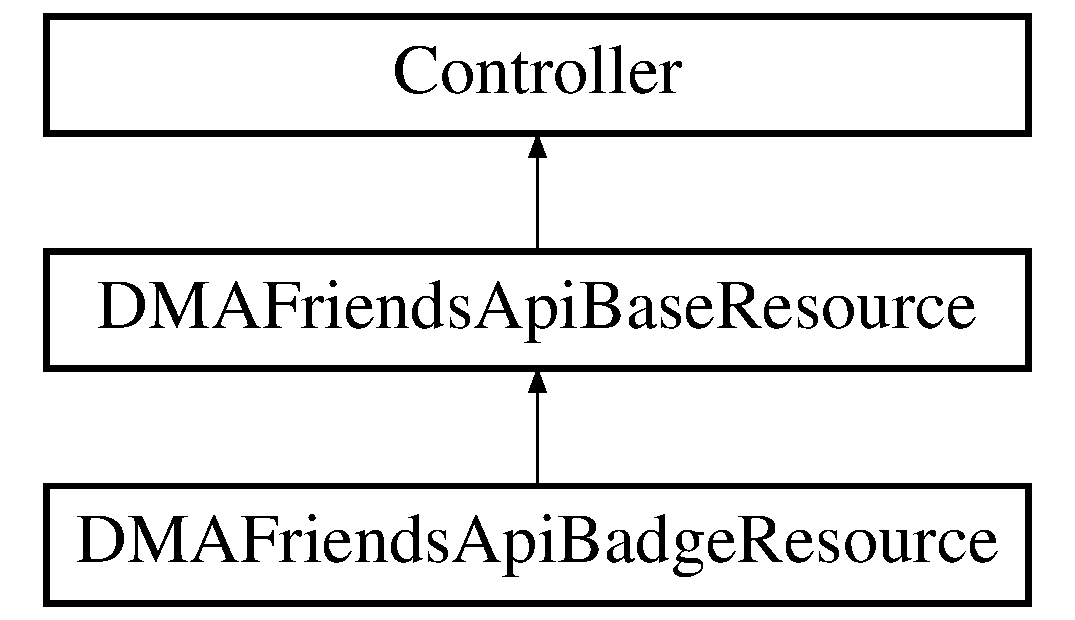
\includegraphics[height=3.000000cm]{d4/d95/classDMA_1_1Friends_1_1Api_1_1BadgeResource}
\end{center}
\end{figure}
\subsection*{Protected Attributes}
\begin{DoxyCompactItemize}
\item 
\hypertarget{classDMA_1_1Friends_1_1Api_1_1BadgeResource_ac4a608f9e0378780c36e0751eb346699}{{\bfseries \$model} = '\textbackslash{}\hyperlink{classDMA_1_1Friends_1_1Models_1_1Badge}{D\-M\-A\textbackslash{}\-Friends\textbackslash{}\-Models\textbackslash{}\-Badge}'}\label{classDMA_1_1Friends_1_1Api_1_1BadgeResource_ac4a608f9e0378780c36e0751eb346699}

\end{DoxyCompactItemize}
\subsection*{Additional Inherited Members}


The documentation for this class was generated from the following file\-:\begin{DoxyCompactItemize}
\item 
api/Badge\-Resource.\-php\end{DoxyCompactItemize}

\hypertarget{classDMA_1_1Friends_1_1Controllers_1_1Badges}{\section{D\-M\-A\textbackslash{}Friends\textbackslash{}Controllers\textbackslash{}Badges Class Reference}
\label{classDMA_1_1Friends_1_1Controllers_1_1Badges}\index{D\-M\-A\textbackslash{}\-Friends\textbackslash{}\-Controllers\textbackslash{}\-Badges@{D\-M\-A\textbackslash{}\-Friends\textbackslash{}\-Controllers\textbackslash{}\-Badges}}
}
Inheritance diagram for D\-M\-A\textbackslash{}Friends\textbackslash{}Controllers\textbackslash{}Badges\-:\begin{figure}[H]
\begin{center}
\leavevmode
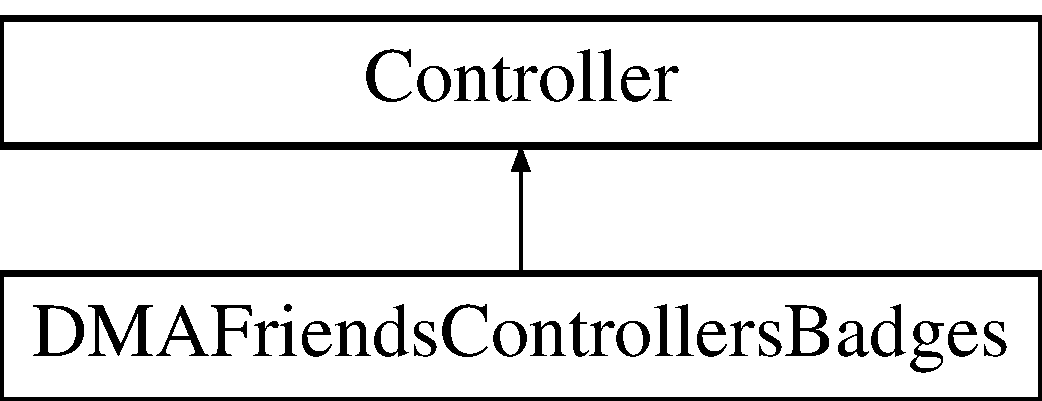
\includegraphics[height=2.000000cm]{d2/d27/classDMA_1_1Friends_1_1Controllers_1_1Badges}
\end{center}
\end{figure}
\subsection*{Public Attributes}
\begin{DoxyCompactItemize}
\item 
{\bfseries \$implement}
\item 
\hypertarget{classDMA_1_1Friends_1_1Controllers_1_1Badges_acc1326493cec81e89163a9f917990fc5}{{\bfseries \$form\-Config} = 'config\-\_\-form.\-yaml'}\label{classDMA_1_1Friends_1_1Controllers_1_1Badges_acc1326493cec81e89163a9f917990fc5}

\item 
\hypertarget{classDMA_1_1Friends_1_1Controllers_1_1Badges_a334b46e1ea9b57d53e297c4a5f93e045}{{\bfseries \$list\-Config} = 'config\-\_\-list.\-yaml'}\label{classDMA_1_1Friends_1_1Controllers_1_1Badges_a334b46e1ea9b57d53e297c4a5f93e045}

\item 
\hypertarget{classDMA_1_1Friends_1_1Controllers_1_1Badges_a70621d9f81b7f23a330e7f08dbdb7ce9}{{\bfseries \$relation\-Config} = 'config\-\_\-relations.\-yaml'}\label{classDMA_1_1Friends_1_1Controllers_1_1Badges_a70621d9f81b7f23a330e7f08dbdb7ce9}

\end{DoxyCompactItemize}


\subsection{Detailed Description}
\hyperlink{classDMA_1_1Friends_1_1Controllers_1_1Badges}{Badges} Back-\/end Controller 

\subsection{Member Data Documentation}
\hypertarget{classDMA_1_1Friends_1_1Controllers_1_1Badges_a77b9d5bec8ddfc58ef42edad23eacac5}{\index{D\-M\-A\-::\-Friends\-::\-Controllers\-::\-Badges@{D\-M\-A\-::\-Friends\-::\-Controllers\-::\-Badges}!\$implement@{\$implement}}
\index{\$implement@{\$implement}!DMA::Friends::Controllers::Badges@{D\-M\-A\-::\-Friends\-::\-Controllers\-::\-Badges}}
\subsubsection[{\$implement}]{\setlength{\rightskip}{0pt plus 5cm}D\-M\-A\textbackslash{}\-Friends\textbackslash{}\-Controllers\textbackslash{}\-Badges\-::\$implement}}\label{classDMA_1_1Friends_1_1Controllers_1_1Badges_a77b9d5bec8ddfc58ef42edad23eacac5}
{\bfseries Initial value\-:}
\begin{DoxyCode}
= [
        \textcolor{stringliteral}{'Backend.Behaviors.FormController'},
        \textcolor{stringliteral}{'Backend.Behaviors.ListController'},
        \textcolor{stringliteral}{'Backend.Behaviors.RelationController'},
    ]
\end{DoxyCode}


The documentation for this class was generated from the following file\-:\begin{DoxyCompactItemize}
\item 
controllers/Badges.\-php\end{DoxyCompactItemize}

\hypertarget{classDMA_1_1Friends_1_1Api_1_1BadgeTransformer}{\section{D\+M\+A\textbackslash{}Friends\textbackslash{}Api\textbackslash{}Badge\+Transformer Class Reference}
\label{classDMA_1_1Friends_1_1Api_1_1BadgeTransformer}\index{D\+M\+A\textbackslash{}\+Friends\textbackslash{}\+Api\textbackslash{}\+Badge\+Transformer@{D\+M\+A\textbackslash{}\+Friends\textbackslash{}\+Api\textbackslash{}\+Badge\+Transformer}}
}
Inheritance diagram for D\+M\+A\textbackslash{}Friends\textbackslash{}Api\textbackslash{}Badge\+Transformer\+:\begin{figure}[H]
\begin{center}
\leavevmode
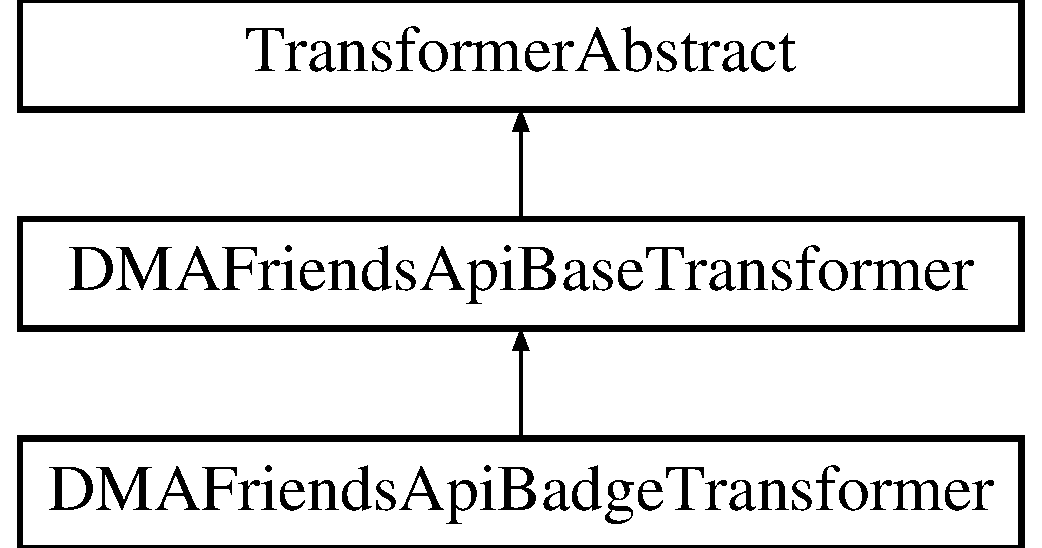
\includegraphics[height=3.000000cm]{dc/db3/classDMA_1_1Friends_1_1Api_1_1BadgeTransformer}
\end{center}
\end{figure}
\subsection*{Additional Inherited Members}


The documentation for this class was generated from the following file\+:\begin{DoxyCompactItemize}
\item 
api/Badge\+Resource.\+php\end{DoxyCompactItemize}

\hypertarget{classDMA_1_1Friends_1_1Api_1_1BaseResource}{\section{D\+M\+A\textbackslash{}Friends\textbackslash{}Api\textbackslash{}Base\+Resource Class Reference}
\label{classDMA_1_1Friends_1_1Api_1_1BaseResource}\index{D\+M\+A\textbackslash{}\+Friends\textbackslash{}\+Api\textbackslash{}\+Base\+Resource@{D\+M\+A\textbackslash{}\+Friends\textbackslash{}\+Api\textbackslash{}\+Base\+Resource}}
}
Inheritance diagram for D\+M\+A\textbackslash{}Friends\textbackslash{}Api\textbackslash{}Base\+Resource\+:\begin{figure}[H]
\begin{center}
\leavevmode
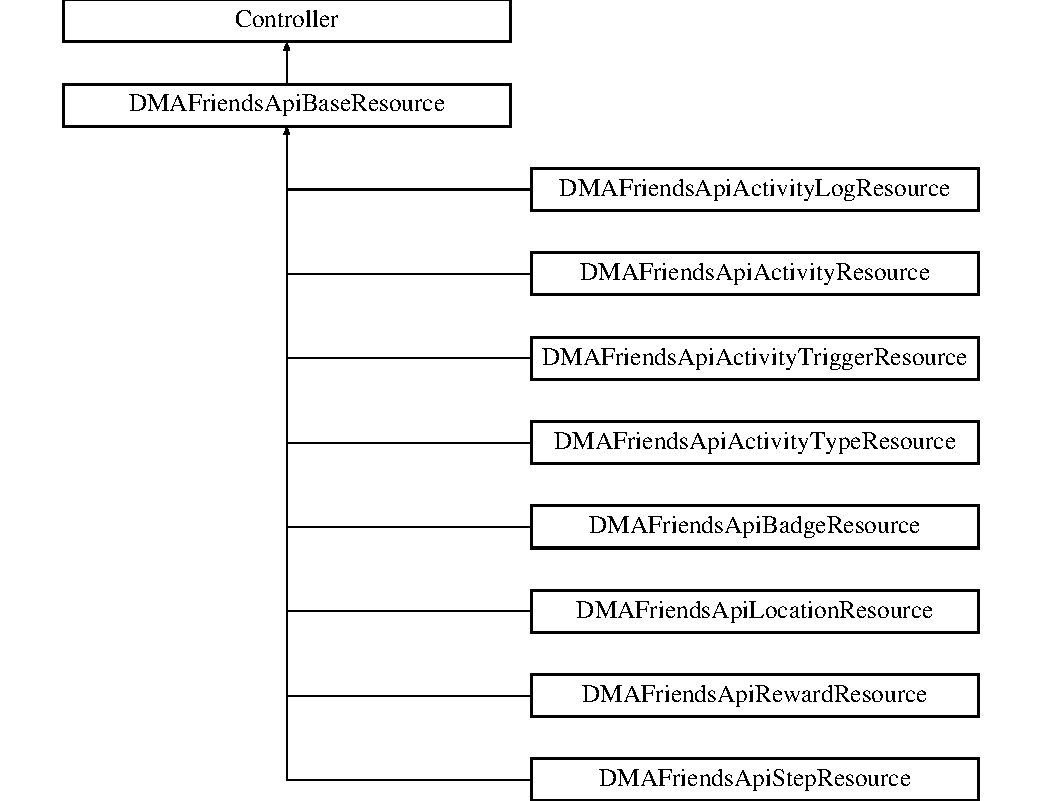
\includegraphics[height=1.000000cm]{d9/dda/classDMA_1_1Friends_1_1Api_1_1BaseResource}
\end{center}
\end{figure}
\subsection*{Public Member Functions}
\begin{DoxyCompactItemize}
\item 
\hyperlink{classDMA_1_1Friends_1_1Api_1_1BaseResource_add87ebd329590ef27490fe6b8ea6f418}{index} ()
\item 
\hyperlink{classDMA_1_1Friends_1_1Api_1_1BaseResource_a2e62ea3d73fab798a5319189b1d134e0}{create} ()
\item 
\hyperlink{classDMA_1_1Friends_1_1Api_1_1BaseResource_a20877c85a440ce26e121a29b8fb91510}{store} ()
\item 
\hyperlink{classDMA_1_1Friends_1_1Api_1_1BaseResource_a5ac5d4fb30ec5434fd685e044c357f97}{show} (\$id)
\item 
\hyperlink{classDMA_1_1Friends_1_1Api_1_1BaseResource_a9421c137919875aaf69b0192cec0737d}{edit} (\$id)
\item 
\hyperlink{classDMA_1_1Friends_1_1Api_1_1BaseResource_a67477f34c9c2d79ef575695c6c426b24}{update} (\$id)
\item 
\hyperlink{classDMA_1_1Friends_1_1Api_1_1BaseResource_a630d3565e6fbec6faff59d8ab79e1e75}{destroy} (\$id)
\end{DoxyCompactItemize}
\subsection*{Protected Attributes}
\begin{DoxyCompactItemize}
\item 
\hypertarget{classDMA_1_1Friends_1_1Api_1_1BaseResource_a2aa14e2ae1346c66fa1522287bd328fc}{{\bfseries \$model}}\label{classDMA_1_1Friends_1_1Api_1_1BaseResource_a2aa14e2ae1346c66fa1522287bd328fc}

\item 
\hypertarget{classDMA_1_1Friends_1_1Api_1_1BaseResource_a2634555f8e0ebf608e538b0d384e0ecd}{{\bfseries \$transformer} = '\hyperlink{classDMA_1_1Friends_1_1Api_1_1BaseTransformer}{D\+M\+A\textbackslash{}\+Friends\textbackslash{}\+Api\textbackslash{}\+Base\+Transformer}'}\label{classDMA_1_1Friends_1_1Api_1_1BaseResource_a2634555f8e0ebf608e538b0d384e0ecd}

\item 
\hypertarget{classDMA_1_1Friends_1_1Api_1_1BaseResource_ac80a10cf9b84009e739d05a502cd3ac8}{{\bfseries \$page\+Size} = 50}\label{classDMA_1_1Friends_1_1Api_1_1BaseResource_ac80a10cf9b84009e739d05a502cd3ac8}

\end{DoxyCompactItemize}


\subsection{Member Function Documentation}
\hypertarget{classDMA_1_1Friends_1_1Api_1_1BaseResource_a2e62ea3d73fab798a5319189b1d134e0}{\index{D\+M\+A\+::\+Friends\+::\+Api\+::\+Base\+Resource@{D\+M\+A\+::\+Friends\+::\+Api\+::\+Base\+Resource}!create@{create}}
\index{create@{create}!D\+M\+A\+::\+Friends\+::\+Api\+::\+Base\+Resource@{D\+M\+A\+::\+Friends\+::\+Api\+::\+Base\+Resource}}
\subsubsection[{create}]{\setlength{\rightskip}{0pt plus 5cm}D\+M\+A\textbackslash{}\+Friends\textbackslash{}\+Api\textbackslash{}\+Base\+Resource\+::create (
\begin{DoxyParamCaption}
{}
\end{DoxyParamCaption}
)}}\label{classDMA_1_1Friends_1_1Api_1_1BaseResource_a2e62ea3d73fab798a5319189b1d134e0}
Show the form for creating a new item

\begin{DoxyReturn}{Returns}
Response 
\end{DoxyReturn}

\begin{DoxyCode}
62     \{
63         \textcolor{keywordflow}{return} $this->errorForbidden();
64     \}
\end{DoxyCode}
\hypertarget{classDMA_1_1Friends_1_1Api_1_1BaseResource_a630d3565e6fbec6faff59d8ab79e1e75}{\index{D\+M\+A\+::\+Friends\+::\+Api\+::\+Base\+Resource@{D\+M\+A\+::\+Friends\+::\+Api\+::\+Base\+Resource}!destroy@{destroy}}
\index{destroy@{destroy}!D\+M\+A\+::\+Friends\+::\+Api\+::\+Base\+Resource@{D\+M\+A\+::\+Friends\+::\+Api\+::\+Base\+Resource}}
\subsubsection[{destroy}]{\setlength{\rightskip}{0pt plus 5cm}D\+M\+A\textbackslash{}\+Friends\textbackslash{}\+Api\textbackslash{}\+Base\+Resource\+::destroy (
\begin{DoxyParamCaption}
\item[{}]{\$id}
\end{DoxyParamCaption}
)}}\label{classDMA_1_1Friends_1_1Api_1_1BaseResource_a630d3565e6fbec6faff59d8ab79e1e75}
Remove the specified item from storage.


\begin{DoxyParams}[1]{Parameters}
int & {\em \$id} & \\
\hline
\end{DoxyParams}
\begin{DoxyReturn}{Returns}
Response 
\end{DoxyReturn}

\begin{DoxyCode}
125     \{
126         \textcolor{keywordflow}{return} Response::api()->errorForbidden();
127 
128     \}   
\end{DoxyCode}
\hypertarget{classDMA_1_1Friends_1_1Api_1_1BaseResource_a9421c137919875aaf69b0192cec0737d}{\index{D\+M\+A\+::\+Friends\+::\+Api\+::\+Base\+Resource@{D\+M\+A\+::\+Friends\+::\+Api\+::\+Base\+Resource}!edit@{edit}}
\index{edit@{edit}!D\+M\+A\+::\+Friends\+::\+Api\+::\+Base\+Resource@{D\+M\+A\+::\+Friends\+::\+Api\+::\+Base\+Resource}}
\subsubsection[{edit}]{\setlength{\rightskip}{0pt plus 5cm}D\+M\+A\textbackslash{}\+Friends\textbackslash{}\+Api\textbackslash{}\+Base\+Resource\+::edit (
\begin{DoxyParamCaption}
\item[{}]{\$id}
\end{DoxyParamCaption}
)}}\label{classDMA_1_1Friends_1_1Api_1_1BaseResource_a9421c137919875aaf69b0192cec0737d}
Show the form for editing the specified item.


\begin{DoxyParams}[1]{Parameters}
int & {\em \$id} & \\
\hline
\end{DoxyParams}
\begin{DoxyReturn}{Returns}
Response 
\end{DoxyReturn}

\begin{DoxyCode}
102     \{
103         \textcolor{keywordflow}{return} Response::api()->errorForbidden();
104     \}
\end{DoxyCode}
\hypertarget{classDMA_1_1Friends_1_1Api_1_1BaseResource_add87ebd329590ef27490fe6b8ea6f418}{\index{D\+M\+A\+::\+Friends\+::\+Api\+::\+Base\+Resource@{D\+M\+A\+::\+Friends\+::\+Api\+::\+Base\+Resource}!index@{index}}
\index{index@{index}!D\+M\+A\+::\+Friends\+::\+Api\+::\+Base\+Resource@{D\+M\+A\+::\+Friends\+::\+Api\+::\+Base\+Resource}}
\subsubsection[{index}]{\setlength{\rightskip}{0pt plus 5cm}D\+M\+A\textbackslash{}\+Friends\textbackslash{}\+Api\textbackslash{}\+Base\+Resource\+::index (
\begin{DoxyParamCaption}
{}
\end{DoxyParamCaption}
)}}\label{classDMA_1_1Friends_1_1Api_1_1BaseResource_add87ebd329590ef27490fe6b8ea6f418}
Display a listing of items

\begin{DoxyReturn}{Returns}
Response 
\end{DoxyReturn}

\begin{DoxyCode}
46     \{
47         $model = $this->getModel();
48         \textcolor{keywordflow}{if} ($this->pageSize > 0)\{
49             $paginator = $model->paginate($this->pageSize);
50             \textcolor{keywordflow}{return} Response::api()->withPaginator(\textcolor{keyword}{new} IlluminatePaginatorAdapter($paginator), \textcolor{keyword}{new} $this->
      transformer);
51         \}\textcolor{keywordflow}{else}\{
52             \textcolor{keywordflow}{return} Response::api()->withCollection($model->all(), \textcolor{keyword}{new} $this->transformer);
53         \}
54     \}
\end{DoxyCode}
\hypertarget{classDMA_1_1Friends_1_1Api_1_1BaseResource_a5ac5d4fb30ec5434fd685e044c357f97}{\index{D\+M\+A\+::\+Friends\+::\+Api\+::\+Base\+Resource@{D\+M\+A\+::\+Friends\+::\+Api\+::\+Base\+Resource}!show@{show}}
\index{show@{show}!D\+M\+A\+::\+Friends\+::\+Api\+::\+Base\+Resource@{D\+M\+A\+::\+Friends\+::\+Api\+::\+Base\+Resource}}
\subsubsection[{show}]{\setlength{\rightskip}{0pt plus 5cm}D\+M\+A\textbackslash{}\+Friends\textbackslash{}\+Api\textbackslash{}\+Base\+Resource\+::show (
\begin{DoxyParamCaption}
\item[{}]{\$id}
\end{DoxyParamCaption}
)}}\label{classDMA_1_1Friends_1_1Api_1_1BaseResource_a5ac5d4fb30ec5434fd685e044c357f97}
Display the specified item.


\begin{DoxyParams}[1]{Parameters}
int & {\em \$id} & \\
\hline
\end{DoxyParams}
\begin{DoxyReturn}{Returns}
Response 
\end{DoxyReturn}

\begin{DoxyCode}
83     \{
84         \textcolor{keywordflow}{try} \{
85             $model = $this->getModel();
86             $instance = $model->findOrFail($id);    
87             \textcolor{keywordflow}{return} Response::api()->withItem($instance, \textcolor{keyword}{new} $this->transformer);
88         \}\textcolor{keywordflow}{catch}(ModelNotFoundException $e) \{
89             \textcolor{keywordflow}{return} Response::api()->errorNotFound();
90         \}\textcolor{keywordflow}{catch}(Exception $e)\{
91             \textcolor{keywordflow}{return} Response::api()->errorInternalError();
92         \}
93     \}
\end{DoxyCode}
\hypertarget{classDMA_1_1Friends_1_1Api_1_1BaseResource_a20877c85a440ce26e121a29b8fb91510}{\index{D\+M\+A\+::\+Friends\+::\+Api\+::\+Base\+Resource@{D\+M\+A\+::\+Friends\+::\+Api\+::\+Base\+Resource}!store@{store}}
\index{store@{store}!D\+M\+A\+::\+Friends\+::\+Api\+::\+Base\+Resource@{D\+M\+A\+::\+Friends\+::\+Api\+::\+Base\+Resource}}
\subsubsection[{store}]{\setlength{\rightskip}{0pt plus 5cm}D\+M\+A\textbackslash{}\+Friends\textbackslash{}\+Api\textbackslash{}\+Base\+Resource\+::store (
\begin{DoxyParamCaption}
{}
\end{DoxyParamCaption}
)}}\label{classDMA_1_1Friends_1_1Api_1_1BaseResource_a20877c85a440ce26e121a29b8fb91510}
Store a newly created item in storage.

\begin{DoxyReturn}{Returns}
Response 
\end{DoxyReturn}

\begin{DoxyCode}
72     \{
73         \textcolor{keywordflow}{return} $this->errorForbidden();
74     \}
\end{DoxyCode}
\hypertarget{classDMA_1_1Friends_1_1Api_1_1BaseResource_a67477f34c9c2d79ef575695c6c426b24}{\index{D\+M\+A\+::\+Friends\+::\+Api\+::\+Base\+Resource@{D\+M\+A\+::\+Friends\+::\+Api\+::\+Base\+Resource}!update@{update}}
\index{update@{update}!D\+M\+A\+::\+Friends\+::\+Api\+::\+Base\+Resource@{D\+M\+A\+::\+Friends\+::\+Api\+::\+Base\+Resource}}
\subsubsection[{update}]{\setlength{\rightskip}{0pt plus 5cm}D\+M\+A\textbackslash{}\+Friends\textbackslash{}\+Api\textbackslash{}\+Base\+Resource\+::update (
\begin{DoxyParamCaption}
\item[{}]{\$id}
\end{DoxyParamCaption}
)}}\label{classDMA_1_1Friends_1_1Api_1_1BaseResource_a67477f34c9c2d79ef575695c6c426b24}
Update the specified item in storage.


\begin{DoxyParams}[1]{Parameters}
int & {\em \$id} & \\
\hline
\end{DoxyParams}
\begin{DoxyReturn}{Returns}
Response 
\end{DoxyReturn}

\begin{DoxyCode}
113     \{
114         \textcolor{keywordflow}{return} Response::api()->errorForbidden();
115 
116     \}
\end{DoxyCode}


The documentation for this class was generated from the following file\+:\begin{DoxyCompactItemize}
\item 
api/Base\+Resource.\+php\end{DoxyCompactItemize}

\hypertarget{classDMA_1_1Friends_1_1Api_1_1BaseTransformer}{}\section{D\+M\+A\textbackslash{}Friends\textbackslash{}Api\textbackslash{}Base\+Transformer Class Reference}
\label{classDMA_1_1Friends_1_1Api_1_1BaseTransformer}\index{D\+M\+A\textbackslash{}\+Friends\textbackslash{}\+Api\textbackslash{}\+Base\+Transformer@{D\+M\+A\textbackslash{}\+Friends\textbackslash{}\+Api\textbackslash{}\+Base\+Transformer}}
Inheritance diagram for D\+M\+A\textbackslash{}Friends\textbackslash{}Api\textbackslash{}Base\+Transformer\+:\begin{figure}[H]
\begin{center}
\leavevmode
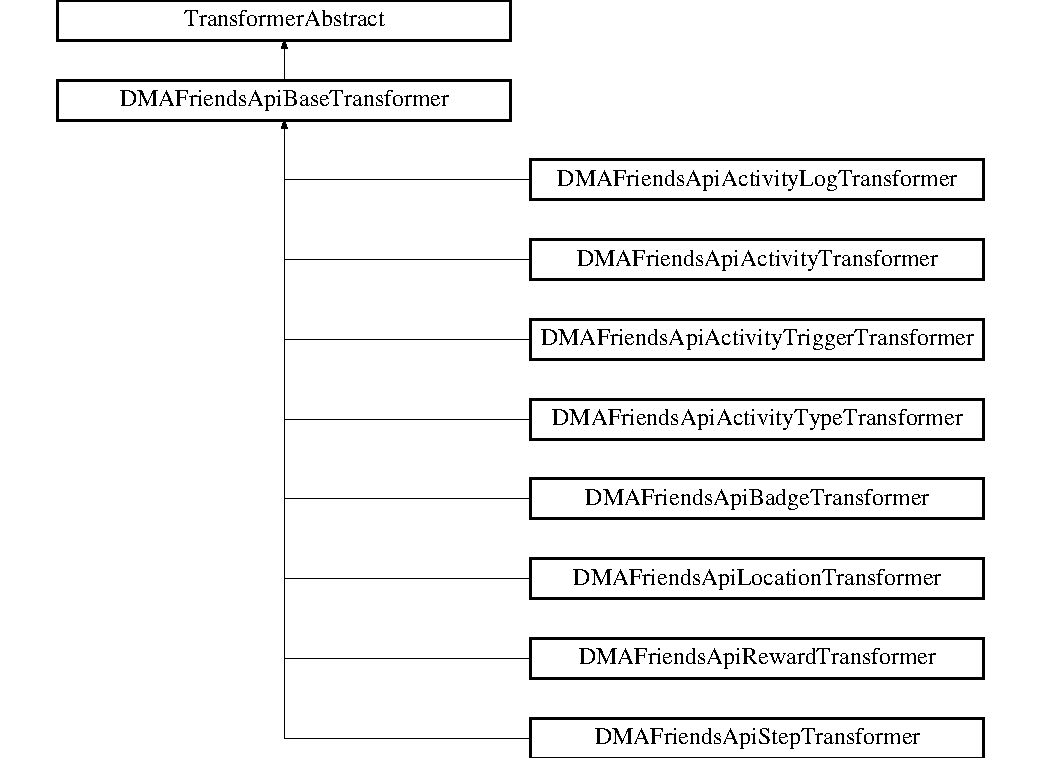
\includegraphics[height=0.941177cm]{d8/dca/classDMA_1_1Friends_1_1Api_1_1BaseTransformer}
\end{center}
\end{figure}
\subsection*{Public Member Functions}
\begin{DoxyCompactItemize}
\item 
\hypertarget{classDMA_1_1Friends_1_1Api_1_1BaseTransformer_a5f1f515afc15dabdd735a09b1dedc248}{}{\bfseries transform} (Model \$instance)\label{classDMA_1_1Friends_1_1Api_1_1BaseTransformer_a5f1f515afc15dabdd735a09b1dedc248}

\end{DoxyCompactItemize}


The documentation for this class was generated from the following file\+:\begin{DoxyCompactItemize}
\item 
api/Base\+Resource.\+php\end{DoxyCompactItemize}

\hypertarget{classDMA_1_1Friends_1_1Classes_1_1FriendsEventHandler}{}\section{D\+M\+A\textbackslash{}Friends\textbackslash{}Classes\textbackslash{}Friends\+Event\+Handler Class Reference}
\label{classDMA_1_1Friends_1_1Classes_1_1FriendsEventHandler}\index{D\+M\+A\textbackslash{}\+Friends\textbackslash{}\+Classes\textbackslash{}\+Friends\+Event\+Handler@{D\+M\+A\textbackslash{}\+Friends\textbackslash{}\+Classes\textbackslash{}\+Friends\+Event\+Handler}}
\subsection*{Public Member Functions}
\begin{DoxyCompactItemize}
\item 
\hyperlink{classDMA_1_1Friends_1_1Classes_1_1FriendsEventHandler_a6467365017b9d494122c8ded41a9a406}{on\+Activity\+Completed} (\$activity, \$user)
\item 
\hyperlink{classDMA_1_1Friends_1_1Classes_1_1FriendsEventHandler_aa13c2568369d06c2a0ca1c96f099ff09}{on\+Badge\+Completed} (\$badge, \$user)
\item 
\hyperlink{classDMA_1_1Friends_1_1Classes_1_1FriendsEventHandler_aeb8499a09334c87311a7f5840c43685a}{on\+Reward\+Redeemed} (\$reward, \$user)
\item 
\hyperlink{classDMA_1_1Friends_1_1Classes_1_1FriendsEventHandler_a3a99cae5eaa37efa395ef4fe8eb30c11}{on\+Step\+Completed} (\$step, \$user)
\item 
\hypertarget{classDMA_1_1Friends_1_1Classes_1_1FriendsEventHandler_a480d5807466962402ccc13260cfb0930}{}{\bfseries on\+Auth\+Login} (\$event)\label{classDMA_1_1Friends_1_1Classes_1_1FriendsEventHandler_a480d5807466962402ccc13260cfb0930}

\item 
\hypertarget{classDMA_1_1Friends_1_1Classes_1_1FriendsEventHandler_aa1d57544bd13c8acf91a3f4e3bf150a5}{}{\bfseries on\+Auth\+Register} (\$user)\label{classDMA_1_1Friends_1_1Classes_1_1FriendsEventHandler_aa1d57544bd13c8acf91a3f4e3bf150a5}

\item 
\hypertarget{classDMA_1_1Friends_1_1Classes_1_1FriendsEventHandler_ac411d3e487b4a16bd3116f3abf1e38a7}{}{\bfseries on\+Notifications\+Ready} ()\label{classDMA_1_1Friends_1_1Classes_1_1FriendsEventHandler_ac411d3e487b4a16bd3116f3abf1e38a7}

\item 
\hypertarget{classDMA_1_1Friends_1_1Classes_1_1FriendsEventHandler_a92cad97622be6dd1ed477dcc05d81074}{}{\bfseries subscribe} (\$events)\label{classDMA_1_1Friends_1_1Classes_1_1FriendsEventHandler_a92cad97622be6dd1ed477dcc05d81074}

\end{DoxyCompactItemize}


\subsection{Member Function Documentation}
\hypertarget{classDMA_1_1Friends_1_1Classes_1_1FriendsEventHandler_a6467365017b9d494122c8ded41a9a406}{}\index{D\+M\+A\+::\+Friends\+::\+Classes\+::\+Friends\+Event\+Handler@{D\+M\+A\+::\+Friends\+::\+Classes\+::\+Friends\+Event\+Handler}!on\+Activity\+Completed@{on\+Activity\+Completed}}
\index{on\+Activity\+Completed@{on\+Activity\+Completed}!D\+M\+A\+::\+Friends\+::\+Classes\+::\+Friends\+Event\+Handler@{D\+M\+A\+::\+Friends\+::\+Classes\+::\+Friends\+Event\+Handler}}
\subsubsection[{on\+Activity\+Completed}]{\setlength{\rightskip}{0pt plus 5cm}D\+M\+A\textbackslash{}\+Friends\textbackslash{}\+Classes\textbackslash{}\+Friends\+Event\+Handler\+::on\+Activity\+Completed (
\begin{DoxyParamCaption}
\item[{}]{\$activity, }
\item[{}]{\$user}
\end{DoxyParamCaption}
)}\label{classDMA_1_1Friends_1_1Classes_1_1FriendsEventHandler_a6467365017b9d494122c8ded41a9a406}
Handle the dma.\+friends.\+activity.\+completed event 
\begin{DoxyParams}[1]{Parameters}
Activity & {\em \$activity} & The activity model that has just been completed \\
\hline
User & {\em \$user} & The user that completed the activity \\
\hline
\end{DoxyParams}

\begin{DoxyCode}
40     \{   
41     \}
\end{DoxyCode}
\hypertarget{classDMA_1_1Friends_1_1Classes_1_1FriendsEventHandler_aa13c2568369d06c2a0ca1c96f099ff09}{}\index{D\+M\+A\+::\+Friends\+::\+Classes\+::\+Friends\+Event\+Handler@{D\+M\+A\+::\+Friends\+::\+Classes\+::\+Friends\+Event\+Handler}!on\+Badge\+Completed@{on\+Badge\+Completed}}
\index{on\+Badge\+Completed@{on\+Badge\+Completed}!D\+M\+A\+::\+Friends\+::\+Classes\+::\+Friends\+Event\+Handler@{D\+M\+A\+::\+Friends\+::\+Classes\+::\+Friends\+Event\+Handler}}
\subsubsection[{on\+Badge\+Completed}]{\setlength{\rightskip}{0pt plus 5cm}D\+M\+A\textbackslash{}\+Friends\textbackslash{}\+Classes\textbackslash{}\+Friends\+Event\+Handler\+::on\+Badge\+Completed (
\begin{DoxyParamCaption}
\item[{}]{\$badge, }
\item[{}]{\$user}
\end{DoxyParamCaption}
)}\label{classDMA_1_1Friends_1_1Classes_1_1FriendsEventHandler_aa13c2568369d06c2a0ca1c96f099ff09}
Handle the dma.\+friends.\+badge.\+completed event 
\begin{DoxyParams}[1]{Parameters}
Badge & {\em \$badge} & The badge model that has just been completed \\
\hline
User & {\em \$user} & The user that completed the badge \\
\hline
\end{DoxyParams}

\begin{DoxyCode}
51     \{
52         \textcolor{keywordflow}{if} (Settings::get(\textcolor{stringliteral}{'send\_badge\_email'})) \{
53             $data = [
54                 \textcolor{stringliteral}{'badge'} => $badge,
55                 \textcolor{stringliteral}{'user'}  => $user,
56             ];
57 
58             Mail::send(\textcolor{stringliteral}{'dma.friends::mail.badge'}, $data, \textcolor{keyword}{function}($message) use ($user)
59             \{
60                 $message->to($user->email, $user->full\_name);
61             \});
62         \}
63     \}
\end{DoxyCode}
\hypertarget{classDMA_1_1Friends_1_1Classes_1_1FriendsEventHandler_aeb8499a09334c87311a7f5840c43685a}{}\index{D\+M\+A\+::\+Friends\+::\+Classes\+::\+Friends\+Event\+Handler@{D\+M\+A\+::\+Friends\+::\+Classes\+::\+Friends\+Event\+Handler}!on\+Reward\+Redeemed@{on\+Reward\+Redeemed}}
\index{on\+Reward\+Redeemed@{on\+Reward\+Redeemed}!D\+M\+A\+::\+Friends\+::\+Classes\+::\+Friends\+Event\+Handler@{D\+M\+A\+::\+Friends\+::\+Classes\+::\+Friends\+Event\+Handler}}
\subsubsection[{on\+Reward\+Redeemed}]{\setlength{\rightskip}{0pt plus 5cm}D\+M\+A\textbackslash{}\+Friends\textbackslash{}\+Classes\textbackslash{}\+Friends\+Event\+Handler\+::on\+Reward\+Redeemed (
\begin{DoxyParamCaption}
\item[{}]{\$reward, }
\item[{}]{\$user}
\end{DoxyParamCaption}
)}\label{classDMA_1_1Friends_1_1Classes_1_1FriendsEventHandler_aeb8499a09334c87311a7f5840c43685a}
Handle the dma.\+friends.\+reward.\+redeemed event 
\begin{DoxyParams}[1]{Parameters}
Reward & {\em \$reward} & The reward model that has just been redeemed \\
\hline
User & {\em \$user} & The user that redeemed the reward \\
\hline
\end{DoxyParams}

\begin{DoxyCode}
73     \{   
74         $data = [
75             \textcolor{stringliteral}{'reward'}    => $reward,
76             \textcolor{stringliteral}{'user'}      => $user,
77         ];
78 
79         \textcolor{comment}{// Send an email to the user that redeemed the reward}
80         \textcolor{keywordflow}{if} ($reward->enable\_email) \{ 
81             Mail::send($reward->email\_template, $data, \textcolor{keyword}{function}($message) use ($reward, $user)
82             \{
83                 $message->to($user->email, $user->full\_name);
84             \});
85         \}
86 
87         \textcolor{keywordflow}{if} ($reward->enable\_admin\_email) \{
88             Mail::send($reward->admin\_email\_template, $data, \textcolor{keyword}{function}($message) use ($reward, $user)
89             \{
90                 \textcolor{comment}{// If a group is configured email those users}
91                 \textcolor{keywordflow}{if} (!empty($reward->admin\_email\_group)) \{
92                     $group = UserGroup::find($reward->admin\_email\_group);
93 
94                     foreach($group->users as $user) \{
95                         $message->to($user->email, $user->first\_name . \textcolor{stringliteral}{' '} . $user->last\_name);
96                     \}
97                 \}
98 
99                 \textcolor{comment}{// If an individual email is configured email that person}
100                 \textcolor{keywordflow}{if} (!empty($reward->admin\_email\_address)) \{
101                     $message->to($reward->admin\_email\_address, \textcolor{stringliteral}{'Anonymous'});
102                 \}
103             \});
104         \}
105 
106         \textcolor{comment}{// Print the reward if user is at a kiosk}
107         $location = LocationManager::getLocation();
108 
109         \textcolor{keywordflow}{if} ($location) \{
110             $printManager = \textcolor{keyword}{new} PrintManager($location, $user);
111             $printManager->printCoupon($reward);
112         \}
113 
114     \}   
\end{DoxyCode}
\hypertarget{classDMA_1_1Friends_1_1Classes_1_1FriendsEventHandler_a3a99cae5eaa37efa395ef4fe8eb30c11}{}\index{D\+M\+A\+::\+Friends\+::\+Classes\+::\+Friends\+Event\+Handler@{D\+M\+A\+::\+Friends\+::\+Classes\+::\+Friends\+Event\+Handler}!on\+Step\+Completed@{on\+Step\+Completed}}
\index{on\+Step\+Completed@{on\+Step\+Completed}!D\+M\+A\+::\+Friends\+::\+Classes\+::\+Friends\+Event\+Handler@{D\+M\+A\+::\+Friends\+::\+Classes\+::\+Friends\+Event\+Handler}}
\subsubsection[{on\+Step\+Completed}]{\setlength{\rightskip}{0pt plus 5cm}D\+M\+A\textbackslash{}\+Friends\textbackslash{}\+Classes\textbackslash{}\+Friends\+Event\+Handler\+::on\+Step\+Completed (
\begin{DoxyParamCaption}
\item[{}]{\$step, }
\item[{}]{\$user}
\end{DoxyParamCaption}
)}\label{classDMA_1_1Friends_1_1Classes_1_1FriendsEventHandler_a3a99cae5eaa37efa395ef4fe8eb30c11}
Handle the dma.\+friends.\+step.\+completed event 
\begin{DoxyParams}[1]{Parameters}
Step & {\em \$step} & The step model that has just been completed \\
\hline
User & {\em \$user} & The user that completed the step \\
\hline
\end{DoxyParams}

\begin{DoxyCode}
124     \{   
125         
126     \}   
\end{DoxyCode}


The documentation for this class was generated from the following file\+:\begin{DoxyCompactItemize}
\item 
classes/Friends\+Event\+Handler.\+php\end{DoxyCompactItemize}

\hypertarget{classDMA_1_1Friends_1_1ReportWidgets_1_1FriendsLeaderboard}{\section{D\+M\+A\textbackslash{}Friends\textbackslash{}Report\+Widgets\textbackslash{}Friends\+Leaderboard Class Reference}
\label{classDMA_1_1Friends_1_1ReportWidgets_1_1FriendsLeaderboard}\index{D\+M\+A\textbackslash{}\+Friends\textbackslash{}\+Report\+Widgets\textbackslash{}\+Friends\+Leaderboard@{D\+M\+A\textbackslash{}\+Friends\textbackslash{}\+Report\+Widgets\textbackslash{}\+Friends\+Leaderboard}}
}
Inheritance diagram for D\+M\+A\textbackslash{}Friends\textbackslash{}Report\+Widgets\textbackslash{}Friends\+Leaderboard\+:\begin{figure}[H]
\begin{center}
\leavevmode
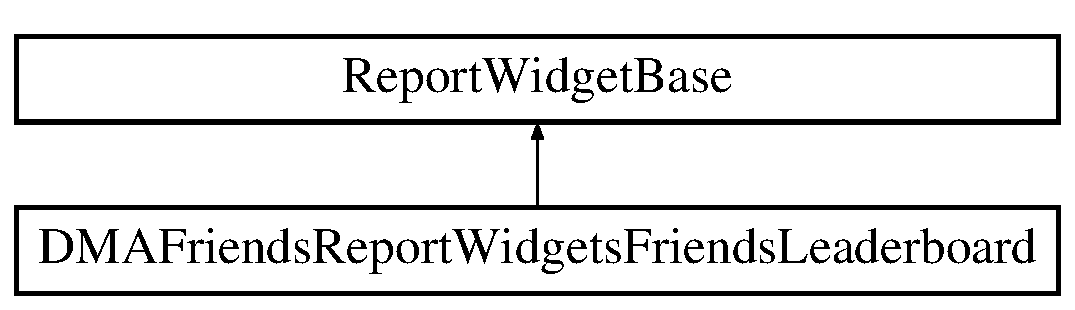
\includegraphics[height=2.000000cm]{dd/dbd/classDMA_1_1Friends_1_1ReportWidgets_1_1FriendsLeaderboard}
\end{center}
\end{figure}
\subsection*{Public Member Functions}
\begin{DoxyCompactItemize}
\item 
\hyperlink{classDMA_1_1Friends_1_1ReportWidgets_1_1FriendsLeaderboard_ac5fc1d8631aca255dee64a37ddeed5f6}{widget\+Details} ()
\item 
\hyperlink{classDMA_1_1Friends_1_1ReportWidgets_1_1FriendsLeaderboard_a8a2b873a91fc33c558834423e35da4bc}{define\+Properties} ()
\item 
\hyperlink{classDMA_1_1Friends_1_1ReportWidgets_1_1FriendsLeaderboard_acc5889523847a95eb855e6041c5ef92f}{render} ()
\end{DoxyCompactItemize}
\subsection*{Public Attributes}
\begin{DoxyCompactItemize}
\item 
\hypertarget{classDMA_1_1Friends_1_1ReportWidgets_1_1FriendsLeaderboard_ab1f836744d59c96df00f1fad2cddb01f}{{\bfseries \$default\+Alias} = 'friends\+Leaderboard'}\label{classDMA_1_1Friends_1_1ReportWidgets_1_1FriendsLeaderboard_ab1f836744d59c96df00f1fad2cddb01f}

\end{DoxyCompactItemize}


\subsection{Member Function Documentation}
\hypertarget{classDMA_1_1Friends_1_1ReportWidgets_1_1FriendsLeaderboard_a8a2b873a91fc33c558834423e35da4bc}{\index{D\+M\+A\+::\+Friends\+::\+Report\+Widgets\+::\+Friends\+Leaderboard@{D\+M\+A\+::\+Friends\+::\+Report\+Widgets\+::\+Friends\+Leaderboard}!define\+Properties@{define\+Properties}}
\index{define\+Properties@{define\+Properties}!D\+M\+A\+::\+Friends\+::\+Report\+Widgets\+::\+Friends\+Leaderboard@{D\+M\+A\+::\+Friends\+::\+Report\+Widgets\+::\+Friends\+Leaderboard}}
\subsubsection[{define\+Properties}]{\setlength{\rightskip}{0pt plus 5cm}D\+M\+A\textbackslash{}\+Friends\textbackslash{}\+Report\+Widgets\textbackslash{}\+Friends\+Leaderboard\+::define\+Properties (
\begin{DoxyParamCaption}
{}
\end{DoxyParamCaption}
)}}\label{classDMA_1_1Friends_1_1ReportWidgets_1_1FriendsLeaderboard_a8a2b873a91fc33c558834423e35da4bc}

\begin{DoxyCode}
30     \{
31         \textcolor{keywordflow}{return} [
32             \textcolor{stringliteral}{'limit'} => [
33                 \textcolor{stringliteral}{'title'}             => \textcolor{stringliteral}{'Number of results'},
34                 \textcolor{stringliteral}{'defualt'}           => 10,
35                 \textcolor{stringliteral}{'type'}              => \textcolor{stringliteral}{'string'},
36                 \textcolor{stringliteral}{'validationPattern'} => \textcolor{stringliteral}{'^[0-9]+$'}
37             ],
38         ];
39     \}
\end{DoxyCode}
\hypertarget{classDMA_1_1Friends_1_1ReportWidgets_1_1FriendsLeaderboard_acc5889523847a95eb855e6041c5ef92f}{\index{D\+M\+A\+::\+Friends\+::\+Report\+Widgets\+::\+Friends\+Leaderboard@{D\+M\+A\+::\+Friends\+::\+Report\+Widgets\+::\+Friends\+Leaderboard}!render@{render}}
\index{render@{render}!D\+M\+A\+::\+Friends\+::\+Report\+Widgets\+::\+Friends\+Leaderboard@{D\+M\+A\+::\+Friends\+::\+Report\+Widgets\+::\+Friends\+Leaderboard}}
\subsubsection[{render}]{\setlength{\rightskip}{0pt plus 5cm}D\+M\+A\textbackslash{}\+Friends\textbackslash{}\+Report\+Widgets\textbackslash{}\+Friends\+Leaderboard\+::render (
\begin{DoxyParamCaption}
{}
\end{DoxyParamCaption}
)}}\label{classDMA_1_1Friends_1_1ReportWidgets_1_1FriendsLeaderboard_acc5889523847a95eb855e6041c5ef92f}

\begin{DoxyCode}
45     \{   
46         $limit = $this->property(\textcolor{stringliteral}{'limit'});
47 
48         $users = User::orderBy(\textcolor{stringliteral}{'points'}, \textcolor{stringliteral}{'DESC'})->take($limit)->get();
49         $this->vars[\textcolor{stringliteral}{'users'}] = $users;
50 
51         \textcolor{keywordflow}{return} $this->makePartial(\textcolor{stringliteral}{'widget'});
52     \}   
\end{DoxyCode}
\hypertarget{classDMA_1_1Friends_1_1ReportWidgets_1_1FriendsLeaderboard_ac5fc1d8631aca255dee64a37ddeed5f6}{\index{D\+M\+A\+::\+Friends\+::\+Report\+Widgets\+::\+Friends\+Leaderboard@{D\+M\+A\+::\+Friends\+::\+Report\+Widgets\+::\+Friends\+Leaderboard}!widget\+Details@{widget\+Details}}
\index{widget\+Details@{widget\+Details}!D\+M\+A\+::\+Friends\+::\+Report\+Widgets\+::\+Friends\+Leaderboard@{D\+M\+A\+::\+Friends\+::\+Report\+Widgets\+::\+Friends\+Leaderboard}}
\subsubsection[{widget\+Details}]{\setlength{\rightskip}{0pt plus 5cm}D\+M\+A\textbackslash{}\+Friends\textbackslash{}\+Report\+Widgets\textbackslash{}\+Friends\+Leaderboard\+::widget\+Details (
\begin{DoxyParamCaption}
{}
\end{DoxyParamCaption}
)}}\label{classDMA_1_1Friends_1_1ReportWidgets_1_1FriendsLeaderboard_ac5fc1d8631aca255dee64a37ddeed5f6}

\begin{DoxyCode}
19     \{   
20         \textcolor{keywordflow}{return} [
21             \textcolor{stringliteral}{'name'}        => \textcolor{stringliteral}{'Friends Leaderboard'},
22             \textcolor{stringliteral}{'description'} => \textcolor{stringliteral}{'Show highest ranking friends members by points'}
23         ];  
24     \}   
\end{DoxyCode}


The documentation for this class was generated from the following file\+:\begin{DoxyCompactItemize}
\item 
reportwidgets/Friends\+Leaderboard.\+php\end{DoxyCompactItemize}

\hypertarget{classDMA_1_1Friends_1_1Classes_1_1FriendsLog}{\section{D\+M\+A\textbackslash{}Friends\textbackslash{}Classes\textbackslash{}Friends\+Log Class Reference}
\label{classDMA_1_1Friends_1_1Classes_1_1FriendsLog}\index{D\+M\+A\textbackslash{}\+Friends\textbackslash{}\+Classes\textbackslash{}\+Friends\+Log@{D\+M\+A\textbackslash{}\+Friends\textbackslash{}\+Classes\textbackslash{}\+Friends\+Log}}
}
\subsection*{Static Public Member Functions}
\begin{DoxyCompactItemize}
\item 
static \hyperlink{classDMA_1_1Friends_1_1Classes_1_1FriendsLog_a99a5a2ee4bc69aab07f58308d9cee669}{write} (\$action, array \$params)
\item 
static \hyperlink{classDMA_1_1Friends_1_1Classes_1_1FriendsLog_a0b90db29da51f53991f2dcc1a55f14c7}{activity} (\$params)
\item 
static \hyperlink{classDMA_1_1Friends_1_1Classes_1_1FriendsLog_aa3c63d0a5b1ffcd9f58c03e443a2dc8f}{artwork} (\$params)
\item 
static \hyperlink{classDMA_1_1Friends_1_1Classes_1_1FriendsLog_ae6c33847a3d3f094a3bd27ac2dbbfa72}{checkin} (\$params)
\item 
static \hyperlink{classDMA_1_1Friends_1_1Classes_1_1FriendsLog_a083fa01b3e143ca77bdbb1562db724de}{points} (\$params)
\item 
static \hyperlink{classDMA_1_1Friends_1_1Classes_1_1FriendsLog_a9f38b9c2e3b1c9d36bc7a1247b2571eb}{reward} (\$params)
\item 
static \hyperlink{classDMA_1_1Friends_1_1Classes_1_1FriendsLog_ac7705d4873f6b3156efde3e049a21ca6}{unlocked} (\$params)
\end{DoxyCompactItemize}


\subsection{Member Function Documentation}
\hypertarget{classDMA_1_1Friends_1_1Classes_1_1FriendsLog_a0b90db29da51f53991f2dcc1a55f14c7}{\index{D\+M\+A\+::\+Friends\+::\+Classes\+::\+Friends\+Log@{D\+M\+A\+::\+Friends\+::\+Classes\+::\+Friends\+Log}!activity@{activity}}
\index{activity@{activity}!D\+M\+A\+::\+Friends\+::\+Classes\+::\+Friends\+Log@{D\+M\+A\+::\+Friends\+::\+Classes\+::\+Friends\+Log}}
\subsubsection[{activity}]{\setlength{\rightskip}{0pt plus 5cm}static D\+M\+A\textbackslash{}\+Friends\textbackslash{}\+Classes\textbackslash{}\+Friends\+Log\+::activity (
\begin{DoxyParamCaption}
\item[{}]{\$params}
\end{DoxyParamCaption}
)\hspace{0.3cm}{\ttfamily [static]}}}\label{classDMA_1_1Friends_1_1Classes_1_1FriendsLog_a0b90db29da51f53991f2dcc1a55f14c7}
Log an activity

\$params
\begin{DoxyItemize}
\item (required) user
\item (required) object An array of parameters to log See \hyperlink{classDMA_1_1Friends_1_1Classes_1_1FriendsLog_a99a5a2ee4bc69aab07f58308d9cee669}{write()} for details
\end{DoxyItemize}

\begin{DoxyReturn}{Returns}
void 
\end{DoxyReturn}

\begin{DoxyCode}
65     \{
66         \textcolor{keywordflow}{if} (empty($params[\textcolor{stringliteral}{'user'}]) || empty($params[\textcolor{stringliteral}{'object'}]))
67             \textcolor{keywordflow}{throw} \textcolor{keyword}{new} \hyperlink{namespaceInvalidArgumentException}{InvalidArgumentException}(\textcolor{stringliteral}{'Invalid Parameters'});
68 
69         $params[\textcolor{stringliteral}{'message'}] = Lang::get(\textcolor{stringliteral}{'dma.friends::lang.log.activity'}, [
70             \textcolor{stringliteral}{'name'}          => $params[\textcolor{stringliteral}{'user'}]->name, 
71             \textcolor{stringliteral}{'title'}         => $params[\textcolor{stringliteral}{'object'}]->title,
72             \textcolor{stringliteral}{'points\_earned'} => $params[\textcolor{stringliteral}{'object'}]->\hyperlink{classDMA_1_1Friends_1_1Classes_1_1FriendsLog_a083fa01b3e143ca77bdbb1562db724de}{points},
73         ]);
74 
75         self::write(\textcolor{stringliteral}{'activity'}, $params);
76     \}
\end{DoxyCode}
\hypertarget{classDMA_1_1Friends_1_1Classes_1_1FriendsLog_aa3c63d0a5b1ffcd9f58c03e443a2dc8f}{\index{D\+M\+A\+::\+Friends\+::\+Classes\+::\+Friends\+Log@{D\+M\+A\+::\+Friends\+::\+Classes\+::\+Friends\+Log}!artwork@{artwork}}
\index{artwork@{artwork}!D\+M\+A\+::\+Friends\+::\+Classes\+::\+Friends\+Log@{D\+M\+A\+::\+Friends\+::\+Classes\+::\+Friends\+Log}}
\subsubsection[{artwork}]{\setlength{\rightskip}{0pt plus 5cm}static D\+M\+A\textbackslash{}\+Friends\textbackslash{}\+Classes\textbackslash{}\+Friends\+Log\+::artwork (
\begin{DoxyParamCaption}
\item[{}]{\$params}
\end{DoxyParamCaption}
)\hspace{0.3cm}{\ttfamily [static]}}}\label{classDMA_1_1Friends_1_1Classes_1_1FriendsLog_aa3c63d0a5b1ffcd9f58c03e443a2dc8f}
Log an artwork activity See \hyperlink{classDMA_1_1Friends_1_1Classes_1_1FriendsLog_a99a5a2ee4bc69aab07f58308d9cee669}{write()} for details

\$params An array of parameters to log

\begin{DoxyReturn}{Returns}
void 
\end{DoxyReturn}

\begin{DoxyCode}
88     \{
89         \textcolor{keywordflow}{if} (empty($params[\textcolor{stringliteral}{'user'}]) || empty($params[\textcolor{stringliteral}{'artwork\_id'}]))
90             \textcolor{keywordflow}{throw} \textcolor{keyword}{new} \hyperlink{namespaceInvalidArgumentException}{InvalidArgumentException}(\textcolor{stringliteral}{'Invalid Parameters'});
91 
92         $params[\textcolor{stringliteral}{'message'}] = Lang::get(\textcolor{stringliteral}{'dma.friends::lang.log.artwork'}, [
93             \textcolor{stringliteral}{'name'}          => $params[\textcolor{stringliteral}{'user'}]->name, 
94             \textcolor{stringliteral}{'artwork\_id'}    => $params[\textcolor{stringliteral}{'artwork\_id'}],
95         ]); 
96 
97         self::write(\textcolor{stringliteral}{'artwork'}, $params);
98     \}
\end{DoxyCode}
\hypertarget{classDMA_1_1Friends_1_1Classes_1_1FriendsLog_ae6c33847a3d3f094a3bd27ac2dbbfa72}{\index{D\+M\+A\+::\+Friends\+::\+Classes\+::\+Friends\+Log@{D\+M\+A\+::\+Friends\+::\+Classes\+::\+Friends\+Log}!checkin@{checkin}}
\index{checkin@{checkin}!D\+M\+A\+::\+Friends\+::\+Classes\+::\+Friends\+Log@{D\+M\+A\+::\+Friends\+::\+Classes\+::\+Friends\+Log}}
\subsubsection[{checkin}]{\setlength{\rightskip}{0pt plus 5cm}static D\+M\+A\textbackslash{}\+Friends\textbackslash{}\+Classes\textbackslash{}\+Friends\+Log\+::checkin (
\begin{DoxyParamCaption}
\item[{}]{\$params}
\end{DoxyParamCaption}
)\hspace{0.3cm}{\ttfamily [static]}}}\label{classDMA_1_1Friends_1_1Classes_1_1FriendsLog_ae6c33847a3d3f094a3bd27ac2dbbfa72}
Log a checkin See \hyperlink{classDMA_1_1Friends_1_1Classes_1_1FriendsLog_a99a5a2ee4bc69aab07f58308d9cee669}{write()} for details

\$params An array of parameters to log

\begin{DoxyReturn}{Returns}
void 
\end{DoxyReturn}

\begin{DoxyCode}
110     \{
111         \textcolor{keywordflow}{if} (empty($params[\textcolor{stringliteral}{'user'}]) || empty($params[\textcolor{stringliteral}{'object'}]))
112             \textcolor{keywordflow}{throw} \textcolor{keyword}{new} \hyperlink{namespaceInvalidArgumentException}{InvalidArgumentException}(\textcolor{stringliteral}{'Invalid Parameters'});
113 
114         $params[\textcolor{stringliteral}{'message'}] = Lang::get(\textcolor{stringliteral}{'dma.friends::lang.log.checkin'}, [
115             \textcolor{stringliteral}{'name'}  => $params[\textcolor{stringliteral}{'user'}]->name, 
116             \textcolor{stringliteral}{'title'} => $params[\textcolor{stringliteral}{'object'}]->title
117         ]); 
118 
119         self::write(\textcolor{stringliteral}{'checkin'}, $params);
120     \}
\end{DoxyCode}
\hypertarget{classDMA_1_1Friends_1_1Classes_1_1FriendsLog_a083fa01b3e143ca77bdbb1562db724de}{\index{D\+M\+A\+::\+Friends\+::\+Classes\+::\+Friends\+Log@{D\+M\+A\+::\+Friends\+::\+Classes\+::\+Friends\+Log}!points@{points}}
\index{points@{points}!D\+M\+A\+::\+Friends\+::\+Classes\+::\+Friends\+Log@{D\+M\+A\+::\+Friends\+::\+Classes\+::\+Friends\+Log}}
\subsubsection[{points}]{\setlength{\rightskip}{0pt plus 5cm}static D\+M\+A\textbackslash{}\+Friends\textbackslash{}\+Classes\textbackslash{}\+Friends\+Log\+::points (
\begin{DoxyParamCaption}
\item[{}]{\$params}
\end{DoxyParamCaption}
)\hspace{0.3cm}{\ttfamily [static]}}}\label{classDMA_1_1Friends_1_1Classes_1_1FriendsLog_a083fa01b3e143ca77bdbb1562db724de}
Log when a user has been awarded points See \hyperlink{classDMA_1_1Friends_1_1Classes_1_1FriendsLog_a99a5a2ee4bc69aab07f58308d9cee669}{write()} for details

\$params An array of parameters to log

\begin{DoxyReturn}{Returns}
void 
\end{DoxyReturn}

\begin{DoxyCode}
132     \{
133         \textcolor{keywordflow}{if} (empty($params[\textcolor{stringliteral}{'user'}]) || empty($params[\textcolor{stringliteral}{'points\_earned'}]))
134             \textcolor{keywordflow}{throw} \textcolor{keyword}{new} \hyperlink{namespaceInvalidArgumentException}{InvalidArgumentException}(\textcolor{stringliteral}{'Invalid Parameters'});
135 
136         $params[\textcolor{stringliteral}{'message'}] = Lang::get(\textcolor{stringliteral}{'dma.friends::lang.log.points'}, [
137             \textcolor{stringliteral}{'name'}          => $params[\textcolor{stringliteral}{'user'}]->name, 
138             \textcolor{stringliteral}{'points'}        => $params[\textcolor{stringliteral}{'points\_earned'}],
139             \textcolor{stringliteral}{'total\_points'}  => $params[\textcolor{stringliteral}{'user'}]->\hyperlink{classDMA_1_1Friends_1_1Classes_1_1FriendsLog_a083fa01b3e143ca77bdbb1562db724de}{points},
140         ]); 
141 
142         self::write(\textcolor{stringliteral}{'points'}, $params);
143     \}
\end{DoxyCode}
\hypertarget{classDMA_1_1Friends_1_1Classes_1_1FriendsLog_a9f38b9c2e3b1c9d36bc7a1247b2571eb}{\index{D\+M\+A\+::\+Friends\+::\+Classes\+::\+Friends\+Log@{D\+M\+A\+::\+Friends\+::\+Classes\+::\+Friends\+Log}!reward@{reward}}
\index{reward@{reward}!D\+M\+A\+::\+Friends\+::\+Classes\+::\+Friends\+Log@{D\+M\+A\+::\+Friends\+::\+Classes\+::\+Friends\+Log}}
\subsubsection[{reward}]{\setlength{\rightskip}{0pt plus 5cm}static D\+M\+A\textbackslash{}\+Friends\textbackslash{}\+Classes\textbackslash{}\+Friends\+Log\+::reward (
\begin{DoxyParamCaption}
\item[{}]{\$params}
\end{DoxyParamCaption}
)\hspace{0.3cm}{\ttfamily [static]}}}\label{classDMA_1_1Friends_1_1Classes_1_1FriendsLog_a9f38b9c2e3b1c9d36bc7a1247b2571eb}
Log when a user redeems a reward See \hyperlink{classDMA_1_1Friends_1_1Classes_1_1FriendsLog_a99a5a2ee4bc69aab07f58308d9cee669}{write()} for details

\$params An array of parameters to log

\begin{DoxyReturn}{Returns}
void 
\end{DoxyReturn}

\begin{DoxyCode}
155     \{
156         \textcolor{keywordflow}{if} (empty($params[\textcolor{stringliteral}{'user'}]) || empty($params[\textcolor{stringliteral}{'object'}]))
157             \textcolor{keywordflow}{throw} \textcolor{keyword}{new} \hyperlink{namespaceInvalidArgumentException}{InvalidArgumentException}(\textcolor{stringliteral}{'Invalid Parameters'});
158 
159         $params[\textcolor{stringliteral}{'message'}] = Lang::get(\textcolor{stringliteral}{'dma.friends::lang.log.reward'}, [
160             \textcolor{stringliteral}{'name'}  => $params[\textcolor{stringliteral}{'user'}]->name, 
161             \textcolor{stringliteral}{'title'} => $params[\textcolor{stringliteral}{'object'}]->title
162         ]); 
163 
164         self::write(\textcolor{stringliteral}{'reward'}, $params);
165     \}
\end{DoxyCode}
\hypertarget{classDMA_1_1Friends_1_1Classes_1_1FriendsLog_ac7705d4873f6b3156efde3e049a21ca6}{\index{D\+M\+A\+::\+Friends\+::\+Classes\+::\+Friends\+Log@{D\+M\+A\+::\+Friends\+::\+Classes\+::\+Friends\+Log}!unlocked@{unlocked}}
\index{unlocked@{unlocked}!D\+M\+A\+::\+Friends\+::\+Classes\+::\+Friends\+Log@{D\+M\+A\+::\+Friends\+::\+Classes\+::\+Friends\+Log}}
\subsubsection[{unlocked}]{\setlength{\rightskip}{0pt plus 5cm}static D\+M\+A\textbackslash{}\+Friends\textbackslash{}\+Classes\textbackslash{}\+Friends\+Log\+::unlocked (
\begin{DoxyParamCaption}
\item[{}]{\$params}
\end{DoxyParamCaption}
)\hspace{0.3cm}{\ttfamily [static]}}}\label{classDMA_1_1Friends_1_1Classes_1_1FriendsLog_ac7705d4873f6b3156efde3e049a21ca6}
Log when a user unlocks an achievement See \hyperlink{classDMA_1_1Friends_1_1Classes_1_1FriendsLog_a99a5a2ee4bc69aab07f58308d9cee669}{write()} for details

\$params An array of parameters to log

\begin{DoxyReturn}{Returns}
void 
\end{DoxyReturn}

\begin{DoxyCode}
177     \{
178         \textcolor{keywordflow}{if} (empty($params[\textcolor{stringliteral}{'user'}]) || empty($params[\textcolor{stringliteral}{'object'}]))
179             \textcolor{keywordflow}{throw} \textcolor{keyword}{new} \hyperlink{namespaceInvalidArgumentException}{InvalidArgumentException}(\textcolor{stringliteral}{'Invalid Parameters'});
180 
181         $params[\textcolor{stringliteral}{'message'}] = Lang::get(\textcolor{stringliteral}{'dma.friends::lang.log.unlocked'}, [
182             \textcolor{stringliteral}{'name'}  => $params[\textcolor{stringliteral}{'user'}]->name, 
183             \textcolor{stringliteral}{'title'} => $params[\textcolor{stringliteral}{'object'}]->title
184         ]);  
185 
186         self::write(\textcolor{stringliteral}{'unlocked'}, $params);
187     \}
\end{DoxyCode}
\hypertarget{classDMA_1_1Friends_1_1Classes_1_1FriendsLog_a99a5a2ee4bc69aab07f58308d9cee669}{\index{D\+M\+A\+::\+Friends\+::\+Classes\+::\+Friends\+Log@{D\+M\+A\+::\+Friends\+::\+Classes\+::\+Friends\+Log}!write@{write}}
\index{write@{write}!D\+M\+A\+::\+Friends\+::\+Classes\+::\+Friends\+Log@{D\+M\+A\+::\+Friends\+::\+Classes\+::\+Friends\+Log}}
\subsubsection[{write}]{\setlength{\rightskip}{0pt plus 5cm}static D\+M\+A\textbackslash{}\+Friends\textbackslash{}\+Classes\textbackslash{}\+Friends\+Log\+::write (
\begin{DoxyParamCaption}
\item[{}]{\$action, }
\item[{array}]{\$params}
\end{DoxyParamCaption}
)\hspace{0.3cm}{\ttfamily [static]}}}\label{classDMA_1_1Friends_1_1Classes_1_1FriendsLog_a99a5a2ee4bc69aab07f58308d9cee669}
Write a log entry to the activity log


\begin{DoxyParams}{Parameters}
{\em \$action} & The type of action to be logged\\
\hline
{\em \$params} & An array of parameters about the log entry
\begin{DoxyItemize}
\item 'user'\+: The user object to associate the log entry
\item 'message'\+: A log message
\item (optional) 'object'\+: A database model to associate the log with
\item (optional) 'points\+\_\+earned'\+: The number of points earned by the action
\item (optional) 'artwork\+\_\+id'\+: The assession number of an artwork to associate the log entry 
\end{DoxyItemize}\\
\hline
\end{DoxyParams}

\begin{DoxyCode}
28     \{
29         $log                = \textcolor{keyword}{new} ActivityLog;
30         $log->user          = $params[\textcolor{stringliteral}{'user'}];
31         $log->action        = $action;
32         $log->message       = $params[\textcolor{stringliteral}{'message'}];
33         $log->points\_earned = isset($params[\textcolor{stringliteral}{'points\_earned'}]) ? $params[\textcolor{stringliteral}{'points\_earned'}] : 0;
34         $log->timestamp     = \textcolor{keyword}{new} \hyperlink{namespaceDateTime}{DateTime}(\textcolor{stringliteral}{'now'});
35 
36         \textcolor{keywordflow}{if} (isset($params[\textcolor{stringliteral}{'artwork\_id'}])) \{
37             $log->artwork\_id = $params[\textcolor{stringliteral}{'artwork\_id'}];
38         \}
39 
40         $log->save();
41 
42         \textcolor{comment}{// Associate an object if present}
43         \textcolor{keywordflow}{if} (isset($params[\textcolor{stringliteral}{'object'}]) && !empty($params[\textcolor{stringliteral}{'object'}])) \{
44             $params[\textcolor{stringliteral}{'object'}]->activityLogs()->save($log);
45         \}
46 
47     \}
\end{DoxyCode}


The documentation for this class was generated from the following file\+:\begin{DoxyCompactItemize}
\item 
classes/Friends\+Log.\+php\end{DoxyCompactItemize}

\hypertarget{classDMA_1_1Friends_1_1FriendsServiceProvider}{\section{D\-M\-A\textbackslash{}Friends\textbackslash{}Friends\-Service\-Provider Class Reference}
\label{classDMA_1_1Friends_1_1FriendsServiceProvider}\index{D\-M\-A\textbackslash{}\-Friends\textbackslash{}\-Friends\-Service\-Provider@{D\-M\-A\textbackslash{}\-Friends\textbackslash{}\-Friends\-Service\-Provider}}
}
Inheritance diagram for D\-M\-A\textbackslash{}Friends\textbackslash{}Friends\-Service\-Provider\-:\begin{figure}[H]
\begin{center}
\leavevmode
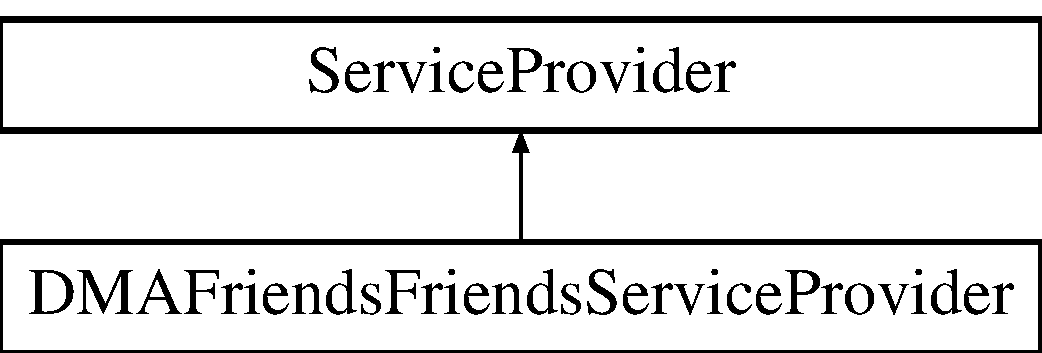
\includegraphics[height=2.000000cm]{df/d6d/classDMA_1_1Friends_1_1FriendsServiceProvider}
\end{center}
\end{figure}
\subsection*{Public Member Functions}
\begin{DoxyCompactItemize}
\item 
\hypertarget{classDMA_1_1Friends_1_1FriendsServiceProvider_a6a90d2cdc4c6b153b45764ba66e154ae}{{\bfseries register} ()}\label{classDMA_1_1Friends_1_1FriendsServiceProvider_a6a90d2cdc4c6b153b45764ba66e154ae}

\item 
\hypertarget{classDMA_1_1Friends_1_1FriendsServiceProvider_acac19246d5282897b8e0ce6265ed5ef3}{{\bfseries register\-Activity\-Processor} ()}\label{classDMA_1_1Friends_1_1FriendsServiceProvider_acac19246d5282897b8e0ce6265ed5ef3}

\item 
\hypertarget{classDMA_1_1Friends_1_1FriendsServiceProvider_a8c3cfb466bb9300f3909797a6b58b634}{{\bfseries register\-Badge\-Processor} ()}\label{classDMA_1_1Friends_1_1FriendsServiceProvider_a8c3cfb466bb9300f3909797a6b58b634}

\item 
\hypertarget{classDMA_1_1Friends_1_1FriendsServiceProvider_a2d6ff7101ca6389c00e298f2d594a1df}{{\bfseries register\-Friends\-Log} ()}\label{classDMA_1_1Friends_1_1FriendsServiceProvider_a2d6ff7101ca6389c00e298f2d594a1df}

\end{DoxyCompactItemize}
\subsection*{Protected Member Functions}
\begin{DoxyCompactItemize}
\item 
\hypertarget{classDMA_1_1Friends_1_1FriendsServiceProvider_acad52dc5020c640afed3c4fe82243051}{{\bfseries create\-Alias} (\$alias, \$class)}\label{classDMA_1_1Friends_1_1FriendsServiceProvider_acad52dc5020c640afed3c4fe82243051}

\end{DoxyCompactItemize}


The documentation for this class was generated from the following file\-:\begin{DoxyCompactItemize}
\item 
Friends\-Service\-Provider.\-php\end{DoxyCompactItemize}

\hypertarget{classDMA_1_1Friends_1_1ReportWidgets_1_1FriendsToolbar}{\section{D\+M\+A\textbackslash{}Friends\textbackslash{}Report\+Widgets\textbackslash{}Friends\+Toolbar Class Reference}
\label{classDMA_1_1Friends_1_1ReportWidgets_1_1FriendsToolbar}\index{D\+M\+A\textbackslash{}\+Friends\textbackslash{}\+Report\+Widgets\textbackslash{}\+Friends\+Toolbar@{D\+M\+A\textbackslash{}\+Friends\textbackslash{}\+Report\+Widgets\textbackslash{}\+Friends\+Toolbar}}
}
Inheritance diagram for D\+M\+A\textbackslash{}Friends\textbackslash{}Report\+Widgets\textbackslash{}Friends\+Toolbar\+:\begin{figure}[H]
\begin{center}
\leavevmode
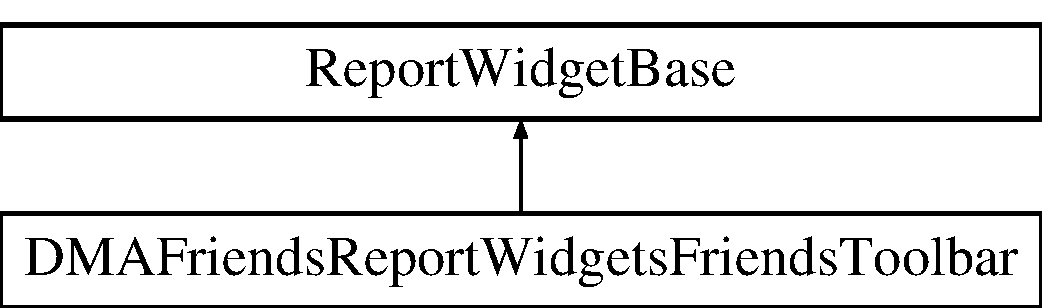
\includegraphics[height=2.000000cm]{d4/d8c/classDMA_1_1Friends_1_1ReportWidgets_1_1FriendsToolbar}
\end{center}
\end{figure}
\subsection*{Public Member Functions}
\begin{DoxyCompactItemize}
\item 
\hypertarget{classDMA_1_1Friends_1_1ReportWidgets_1_1FriendsToolbar_a56951946e166c46353910da4a5c399a1}{{\bfseries widget\+Details} ()}\label{classDMA_1_1Friends_1_1ReportWidgets_1_1FriendsToolbar_a56951946e166c46353910da4a5c399a1}

\item 
\hypertarget{classDMA_1_1Friends_1_1ReportWidgets_1_1FriendsToolbar_a5fb3de1ff5dd5186e068dcf8c5e8d154}{{\bfseries render} ()}\label{classDMA_1_1Friends_1_1ReportWidgets_1_1FriendsToolbar_a5fb3de1ff5dd5186e068dcf8c5e8d154}

\end{DoxyCompactItemize}
\subsection*{Public Attributes}
\begin{DoxyCompactItemize}
\item 
\hypertarget{classDMA_1_1Friends_1_1ReportWidgets_1_1FriendsToolbar_aabef17c5a99fc5f66554a91dd2cde59d}{{\bfseries \$default\+Alias} = 'friends\+Toolbar'}\label{classDMA_1_1Friends_1_1ReportWidgets_1_1FriendsToolbar_aabef17c5a99fc5f66554a91dd2cde59d}

\end{DoxyCompactItemize}


The documentation for this class was generated from the following file\+:\begin{DoxyCompactItemize}
\item 
reportwidgets/Friends\+Toolbar.\+php\end{DoxyCompactItemize}

\hypertarget{classDMA_1_1Friends_1_1Api_1_1GenericModelRepository}{}\section{D\+M\+A\textbackslash{}Friends\textbackslash{}Api\textbackslash{}Generic\+Model\+Repository Class Reference}
\label{classDMA_1_1Friends_1_1Api_1_1GenericModelRepository}\index{D\+M\+A\textbackslash{}\+Friends\textbackslash{}\+Api\textbackslash{}\+Generic\+Model\+Repository@{D\+M\+A\textbackslash{}\+Friends\textbackslash{}\+Api\textbackslash{}\+Generic\+Model\+Repository}}
\subsection*{Public Member Functions}
\begin{DoxyCompactItemize}
\item 
\hypertarget{classDMA_1_1Friends_1_1Api_1_1GenericModelRepository_a320f3591265cbdf46a9c9fa26927df10}{}{\bfseries \+\_\+\+\_\+construct} (\$model\+Class\+Name)\label{classDMA_1_1Friends_1_1Api_1_1GenericModelRepository_a320f3591265cbdf46a9c9fa26927df10}

\item 
\hypertarget{classDMA_1_1Friends_1_1Api_1_1GenericModelRepository_ac0e8251f4383610298dddda3eb7958d7}{}{\bfseries create} (array \$attributes)\label{classDMA_1_1Friends_1_1Api_1_1GenericModelRepository_ac0e8251f4383610298dddda3eb7958d7}

\item 
\hypertarget{classDMA_1_1Friends_1_1Api_1_1GenericModelRepository_a4c88d28c6fc169ae1eead0b0aa3866f9}{}{\bfseries all} (\$columns=array(\textquotesingle{}$\ast$\textquotesingle{}))\label{classDMA_1_1Friends_1_1Api_1_1GenericModelRepository_a4c88d28c6fc169ae1eead0b0aa3866f9}

\item 
\hypertarget{classDMA_1_1Friends_1_1Api_1_1GenericModelRepository_ab42b1bda9479d9990e04c9d45f2a0e0d}{}{\bfseries find} (\$id, \$columns=array(\textquotesingle{}$\ast$\textquotesingle{}))\label{classDMA_1_1Friends_1_1Api_1_1GenericModelRepository_ab42b1bda9479d9990e04c9d45f2a0e0d}

\item 
\hypertarget{classDMA_1_1Friends_1_1Api_1_1GenericModelRepository_a0fe974a6605164516635931f06eb4c30}{}{\bfseries find\+Or\+Fail} (\$id, \$columns=array(\textquotesingle{}$\ast$\textquotesingle{}))\label{classDMA_1_1Friends_1_1Api_1_1GenericModelRepository_a0fe974a6605164516635931f06eb4c30}

\item 
\hypertarget{classDMA_1_1Friends_1_1Api_1_1GenericModelRepository_a82078490bec0c283af63fb52200224a0}{}{\bfseries destroy} (\$ids)\label{classDMA_1_1Friends_1_1Api_1_1GenericModelRepository_a82078490bec0c283af63fb52200224a0}

\item 
\hypertarget{classDMA_1_1Friends_1_1Api_1_1GenericModelRepository_a2d7794ceb5795fef531ad856b36d0daa}{}{\bfseries paginate} (\$per\+Page=null, \$columns=array(\textquotesingle{}$\ast$\textquotesingle{}))\label{classDMA_1_1Friends_1_1Api_1_1GenericModelRepository_a2d7794ceb5795fef531ad856b36d0daa}

\end{DoxyCompactItemize}
\subsection*{Protected Attributes}
\begin{DoxyCompactItemize}
\item 
\hypertarget{classDMA_1_1Friends_1_1Api_1_1GenericModelRepository_a24215ef1696b0dedaf385b16f03ea000}{}{\bfseries \$model\+Class\+Name}\label{classDMA_1_1Friends_1_1Api_1_1GenericModelRepository_a24215ef1696b0dedaf385b16f03ea000}

\end{DoxyCompactItemize}


The documentation for this class was generated from the following file\+:\begin{DoxyCompactItemize}
\item 
api/Base\+Resource.\+php\end{DoxyCompactItemize}

\hypertarget{classDMA_1_1Friends_1_1Models_1_1Location}{\section{D\+M\+A\textbackslash{}Friends\textbackslash{}Models\textbackslash{}Location Class Reference}
\label{classDMA_1_1Friends_1_1Models_1_1Location}\index{D\+M\+A\textbackslash{}\+Friends\textbackslash{}\+Models\textbackslash{}\+Location@{D\+M\+A\textbackslash{}\+Friends\textbackslash{}\+Models\textbackslash{}\+Location}}
}
Inheritance diagram for D\+M\+A\textbackslash{}Friends\textbackslash{}Models\textbackslash{}Location\+:\begin{figure}[H]
\begin{center}
\leavevmode
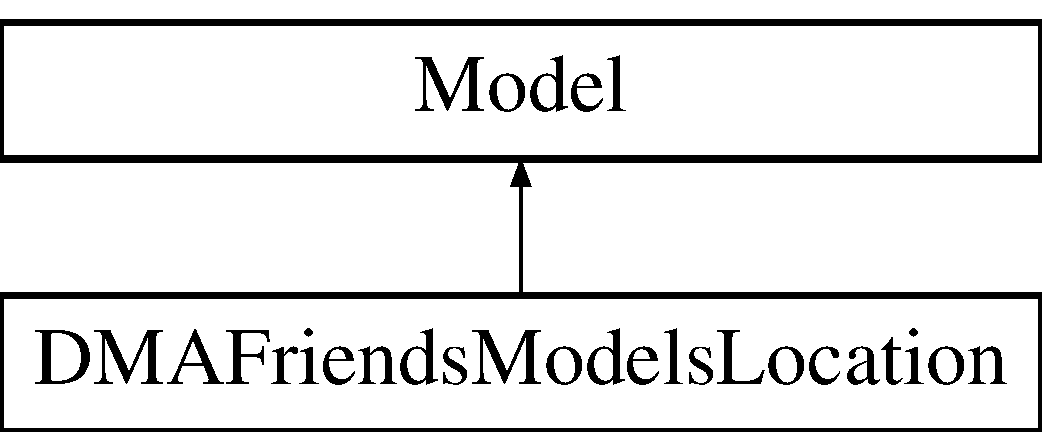
\includegraphics[height=2.000000cm]{d6/df9/classDMA_1_1Friends_1_1Models_1_1Location}
\end{center}
\end{figure}
\subsection*{Public Member Functions}
\begin{DoxyCompactItemize}
\item 
\hypertarget{classDMA_1_1Friends_1_1Models_1_1Location_ad8b1171d787276f812889f20a6916e15}{{\bfseries scopefind\+Wordpress} (\$query, \$id)}\label{classDMA_1_1Friends_1_1Models_1_1Location_ad8b1171d787276f812889f20a6916e15}

\end{DoxyCompactItemize}
\subsection*{Public Attributes}
\begin{DoxyCompactItemize}
\item 
\hypertarget{classDMA_1_1Friends_1_1Models_1_1Location_ac1f41b316e50581d95f80655e36b7f9d}{{\bfseries \$table} = 'dma\+\_\+friends\+\_\+locations'}\label{classDMA_1_1Friends_1_1Models_1_1Location_ac1f41b316e50581d95f80655e36b7f9d}

\item 
\hypertarget{classDMA_1_1Friends_1_1Models_1_1Location_a3df0019a82eb74c240408878329baa2c}{{\bfseries \$rules} = \mbox{[}$\,$\mbox{]}}\label{classDMA_1_1Friends_1_1Models_1_1Location_a3df0019a82eb74c240408878329baa2c}

\item 
{\bfseries \$morph\+Many}
\end{DoxyCompactItemize}
\subsection*{Protected Attributes}
\begin{DoxyCompactItemize}
\item 
\hypertarget{classDMA_1_1Friends_1_1Models_1_1Location_a248021f938f61b3ccce7e20b259e39e9}{{\bfseries \$guarded} = \mbox{[}'$\ast$'\mbox{]}}\label{classDMA_1_1Friends_1_1Models_1_1Location_a248021f938f61b3ccce7e20b259e39e9}

\item 
\hypertarget{classDMA_1_1Friends_1_1Models_1_1Location_aaa75ba74c2a24c4e42b109b0b2c82ca0}{{\bfseries \$fillable} = \mbox{[}$\,$\mbox{]}}\label{classDMA_1_1Friends_1_1Models_1_1Location_aaa75ba74c2a24c4e42b109b0b2c82ca0}

\end{DoxyCompactItemize}


\subsection{Detailed Description}
\hyperlink{classDMA_1_1Friends_1_1Models_1_1Location}{Location} Model 

\subsection{Member Data Documentation}
\hypertarget{classDMA_1_1Friends_1_1Models_1_1Location_a94915d02afa4db52780159b84d9ce12e}{\index{D\+M\+A\+::\+Friends\+::\+Models\+::\+Location@{D\+M\+A\+::\+Friends\+::\+Models\+::\+Location}!\$morph\+Many@{\$morph\+Many}}
\index{\$morph\+Many@{\$morph\+Many}!D\+M\+A\+::\+Friends\+::\+Models\+::\+Location@{D\+M\+A\+::\+Friends\+::\+Models\+::\+Location}}
\subsubsection[{\$morph\+Many}]{\setlength{\rightskip}{0pt plus 5cm}D\+M\+A\textbackslash{}\+Friends\textbackslash{}\+Models\textbackslash{}\+Location\+::\$morph\+Many}}\label{classDMA_1_1Friends_1_1Models_1_1Location_a94915d02afa4db52780159b84d9ce12e}
{\bfseries Initial value\+:}
\begin{DoxyCode}
= [ 
        \textcolor{stringliteral}{'activityLogs'}  => [\textcolor{stringliteral}{'DMA\(\backslash\)Friends\(\backslash\)Models\(\backslash\)ActivityLog'}, \textcolor{stringliteral}{'name'} => \textcolor{stringliteral}{'object'}],
    ]
\end{DoxyCode}


The documentation for this class was generated from the following file\+:\begin{DoxyCompactItemize}
\item 
models/Location.\+php\end{DoxyCompactItemize}

\hypertarget{classDMA_1_1Friends_1_1Wordpress_1_1Location}{\section{D\-M\-A\textbackslash{}Friends\textbackslash{}Wordpress\textbackslash{}Location Class Reference}
\label{classDMA_1_1Friends_1_1Wordpress_1_1Location}\index{D\-M\-A\textbackslash{}\-Friends\textbackslash{}\-Wordpress\textbackslash{}\-Location@{D\-M\-A\textbackslash{}\-Friends\textbackslash{}\-Wordpress\textbackslash{}\-Location}}
}
Inheritance diagram for D\-M\-A\textbackslash{}Friends\textbackslash{}Wordpress\textbackslash{}Location\-:\begin{figure}[H]
\begin{center}
\leavevmode
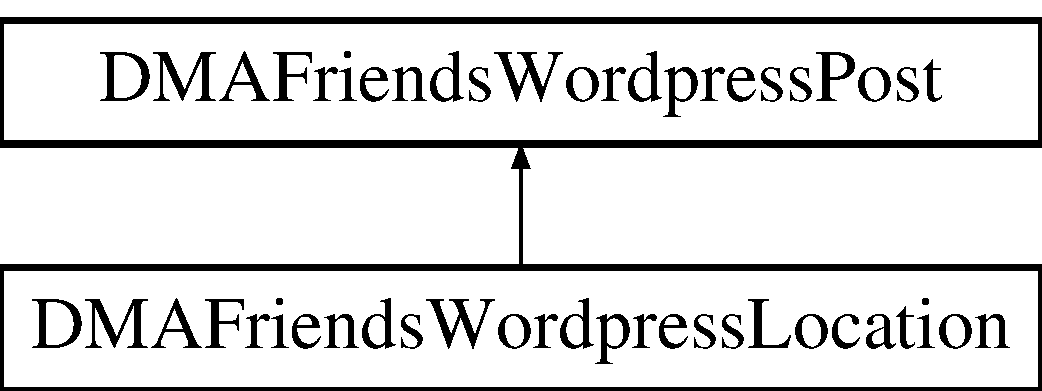
\includegraphics[height=2.000000cm]{d3/d8d/classDMA_1_1Friends_1_1Wordpress_1_1Location}
\end{center}
\end{figure}
\subsection*{Public Attributes}
\begin{DoxyCompactItemize}
\item 
\hypertarget{classDMA_1_1Friends_1_1Wordpress_1_1Location_a40f4ecf15a53d860bfbba3484f2999bf}{{\bfseries \$post\-Type} = 'dma-\/location'}\label{classDMA_1_1Friends_1_1Wordpress_1_1Location_a40f4ecf15a53d860bfbba3484f2999bf}

\end{DoxyCompactItemize}
\subsection*{Protected Attributes}
\begin{DoxyCompactItemize}
\item 
{\bfseries \$exclude\-Fields}
\end{DoxyCompactItemize}
\subsection*{Additional Inherited Members}


\subsection{Member Data Documentation}
\hypertarget{classDMA_1_1Friends_1_1Wordpress_1_1Location_ae18a475210d12a42d335d6ca6fb47811}{\index{D\-M\-A\-::\-Friends\-::\-Wordpress\-::\-Location@{D\-M\-A\-::\-Friends\-::\-Wordpress\-::\-Location}!\$exclude\-Fields@{\$exclude\-Fields}}
\index{\$exclude\-Fields@{\$exclude\-Fields}!DMA::Friends::Wordpress::Location@{D\-M\-A\-::\-Friends\-::\-Wordpress\-::\-Location}}
\subsubsection[{\$exclude\-Fields}]{\setlength{\rightskip}{0pt plus 5cm}D\-M\-A\textbackslash{}\-Friends\textbackslash{}\-Wordpress\textbackslash{}\-Location\-::\$exclude\-Fields\hspace{0.3cm}{\ttfamily [protected]}}}\label{classDMA_1_1Friends_1_1Wordpress_1_1Location_ae18a475210d12a42d335d6ca6fb47811}
{\bfseries Initial value\-:}
\begin{DoxyCode}
= [
        \textcolor{stringliteral}{'post\_excerpt'},
        \textcolor{stringliteral}{'is\_published'},
        \textcolor{stringliteral}{'post\_status'},
    ]
\end{DoxyCode}


The documentation for this class was generated from the following file\-:\begin{DoxyCompactItemize}
\item 
wordpress/Location.\-php\end{DoxyCompactItemize}

\hypertarget{classDMA_1_1Friends_1_1Api_1_1LocationResource}{}\section{D\+M\+A\textbackslash{}Friends\textbackslash{}Api\textbackslash{}Location\+Resource Class Reference}
\label{classDMA_1_1Friends_1_1Api_1_1LocationResource}\index{D\+M\+A\textbackslash{}\+Friends\textbackslash{}\+Api\textbackslash{}\+Location\+Resource@{D\+M\+A\textbackslash{}\+Friends\textbackslash{}\+Api\textbackslash{}\+Location\+Resource}}
Inheritance diagram for D\+M\+A\textbackslash{}Friends\textbackslash{}Api\textbackslash{}Location\+Resource\+:\begin{figure}[H]
\begin{center}
\leavevmode
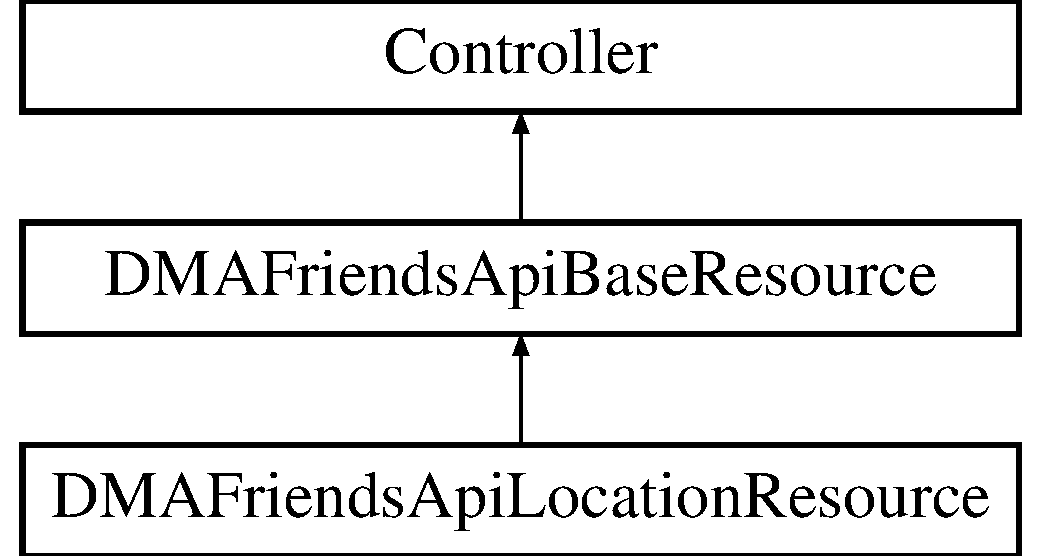
\includegraphics[height=3.000000cm]{d3/d3e/classDMA_1_1Friends_1_1Api_1_1LocationResource}
\end{center}
\end{figure}
\subsection*{Protected Attributes}
\begin{DoxyCompactItemize}
\item 
\hypertarget{classDMA_1_1Friends_1_1Api_1_1LocationResource_a32a593bbeba6c699743670fda7bae672}{}{\bfseries \$model} = \textquotesingle{}\textbackslash{}\hyperlink{classDMA_1_1Friends_1_1Models_1_1Location}{D\+M\+A\textbackslash{}\+Friends\textbackslash{}\+Models\textbackslash{}\+Location}\textquotesingle{}\label{classDMA_1_1Friends_1_1Api_1_1LocationResource_a32a593bbeba6c699743670fda7bae672}

\end{DoxyCompactItemize}
\subsection*{Additional Inherited Members}


The documentation for this class was generated from the following file\+:\begin{DoxyCompactItemize}
\item 
api/Location\+Resource.\+php\end{DoxyCompactItemize}

\hypertarget{classDMA_1_1Friends_1_1Controllers_1_1Locations}{}\section{D\+M\+A\textbackslash{}Friends\textbackslash{}Controllers\textbackslash{}Locations Class Reference}
\label{classDMA_1_1Friends_1_1Controllers_1_1Locations}\index{D\+M\+A\textbackslash{}\+Friends\textbackslash{}\+Controllers\textbackslash{}\+Locations@{D\+M\+A\textbackslash{}\+Friends\textbackslash{}\+Controllers\textbackslash{}\+Locations}}
Inheritance diagram for D\+M\+A\textbackslash{}Friends\textbackslash{}Controllers\textbackslash{}Locations\+:\begin{figure}[H]
\begin{center}
\leavevmode
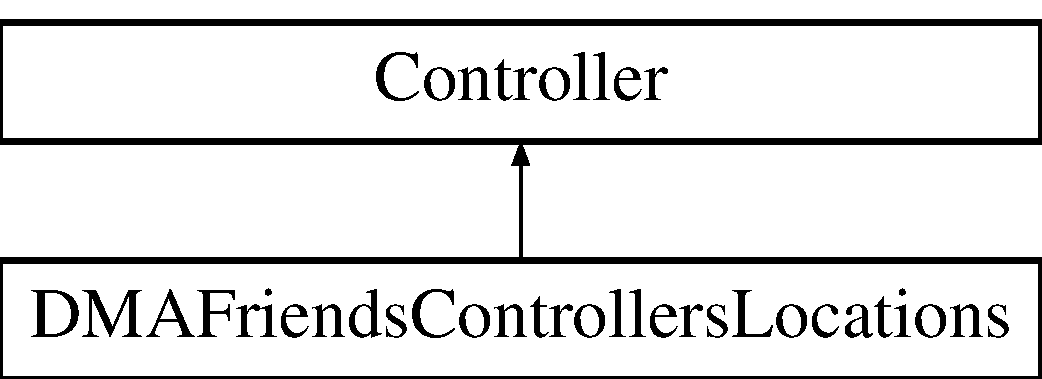
\includegraphics[height=2.000000cm]{d2/d9c/classDMA_1_1Friends_1_1Controllers_1_1Locations}
\end{center}
\end{figure}
\subsection*{Static Public Member Functions}
\begin{DoxyCompactItemize}
\item 
static \hyperlink{classDMA_1_1Friends_1_1Controllers_1_1Locations_a9b6fce6b3f0cf4fe6671fe110b0c8791}{barcode\+Login} ()
\end{DoxyCompactItemize}
\subsection*{Public Attributes}
\begin{DoxyCompactItemize}
\item 
{\bfseries \$implement}
\item 
\hypertarget{classDMA_1_1Friends_1_1Controllers_1_1Locations_a8a769617e49a5e862fa8633b75467223}{}{\bfseries \$form\+Config} = \textquotesingle{}config\+\_\+form.\+yaml\textquotesingle{}\label{classDMA_1_1Friends_1_1Controllers_1_1Locations_a8a769617e49a5e862fa8633b75467223}

\item 
\hypertarget{classDMA_1_1Friends_1_1Controllers_1_1Locations_a54b41dd09d63dafca0bff7528a8c27e1}{}{\bfseries \$list\+Config} = \textquotesingle{}config\+\_\+list.\+yaml\textquotesingle{}\label{classDMA_1_1Friends_1_1Controllers_1_1Locations_a54b41dd09d63dafca0bff7528a8c27e1}

\end{DoxyCompactItemize}


\subsection{Detailed Description}
\hyperlink{classDMA_1_1Friends_1_1Controllers_1_1Locations}{Locations} Back-\/end Controller 

\subsection{Member Function Documentation}
\hypertarget{classDMA_1_1Friends_1_1Controllers_1_1Locations_a9b6fce6b3f0cf4fe6671fe110b0c8791}{}\index{D\+M\+A\+::\+Friends\+::\+Controllers\+::\+Locations@{D\+M\+A\+::\+Friends\+::\+Controllers\+::\+Locations}!barcode\+Login@{barcode\+Login}}
\index{barcode\+Login@{barcode\+Login}!D\+M\+A\+::\+Friends\+::\+Controllers\+::\+Locations@{D\+M\+A\+::\+Friends\+::\+Controllers\+::\+Locations}}
\subsubsection[{barcode\+Login}]{\setlength{\rightskip}{0pt plus 5cm}static D\+M\+A\textbackslash{}\+Friends\textbackslash{}\+Controllers\textbackslash{}\+Locations\+::barcode\+Login (
\begin{DoxyParamCaption}
{}
\end{DoxyParamCaption}
)\hspace{0.3cm}{\ttfamily [static]}}\label{classDMA_1_1Friends_1_1Controllers_1_1Locations_a9b6fce6b3f0cf4fe6671fe110b0c8791}
Resource to login user via barcode scanner for authorized kiosks 
\begin{DoxyCode}
43     \{
44         $barcodeId = \textcolor{keyword}{get}(\textcolor{stringliteral}{'barcodeId'});
45         $barcodeId = trim($barcodeId);
46 
47         $location = LocationManager::getLocation();
48 
49         \textcolor{keywordflow}{if} (!$location || empty($barcodeId)) \{
50             \textcolor{keywordflow}{return} Redirect::to(\textcolor{charliteral}{'/'});
51         \}
52 
53         \textcolor{keywordflow}{if} ($location->is\_authorized) \{
54 
55             $data = [
56                 \textcolor{stringliteral}{'login'}         => $barcodeId,
57                 \textcolor{stringliteral}{'no\_password'}   => \textcolor{keyword}{true},
58             ];
59 
60             \hyperlink{classDMA_1_1Friends_1_1Classes_1_1AuthManager_a22836fc33b7788f7b41bbb253c6f58af}{AuthManager::auth}($data);
61 
62         \}
63 
64         \textcolor{keywordflow}{return} Redirect::to(\textcolor{charliteral}{'/'});
65     \}
\end{DoxyCode}


\subsection{Member Data Documentation}
\hypertarget{classDMA_1_1Friends_1_1Controllers_1_1Locations_a39d07c1344f282eb2d164b92d6df5c8d}{}\index{D\+M\+A\+::\+Friends\+::\+Controllers\+::\+Locations@{D\+M\+A\+::\+Friends\+::\+Controllers\+::\+Locations}!\$implement@{\$implement}}
\index{\$implement@{\$implement}!D\+M\+A\+::\+Friends\+::\+Controllers\+::\+Locations@{D\+M\+A\+::\+Friends\+::\+Controllers\+::\+Locations}}
\subsubsection[{\$implement}]{\setlength{\rightskip}{0pt plus 5cm}D\+M\+A\textbackslash{}\+Friends\textbackslash{}\+Controllers\textbackslash{}\+Locations\+::\$implement}\label{classDMA_1_1Friends_1_1Controllers_1_1Locations_a39d07c1344f282eb2d164b92d6df5c8d}
{\bfseries Initial value\+:}
\begin{DoxyCode}
= [
        \textcolor{stringliteral}{'Backend.Behaviors.FormController'},
        \textcolor{stringliteral}{'Backend.Behaviors.ListController'}
    ]
\end{DoxyCode}


The documentation for this class was generated from the following file\+:\begin{DoxyCompactItemize}
\item 
controllers/Locations.\+php\end{DoxyCompactItemize}

\hypertarget{classDMA_1_1Friends_1_1Api_1_1LocationTransformer}{}\section{D\+M\+A\textbackslash{}Friends\textbackslash{}Api\textbackslash{}Location\+Transformer Class Reference}
\label{classDMA_1_1Friends_1_1Api_1_1LocationTransformer}\index{D\+M\+A\textbackslash{}\+Friends\textbackslash{}\+Api\textbackslash{}\+Location\+Transformer@{D\+M\+A\textbackslash{}\+Friends\textbackslash{}\+Api\textbackslash{}\+Location\+Transformer}}
Inheritance diagram for D\+M\+A\textbackslash{}Friends\textbackslash{}Api\textbackslash{}Location\+Transformer\+:\begin{figure}[H]
\begin{center}
\leavevmode
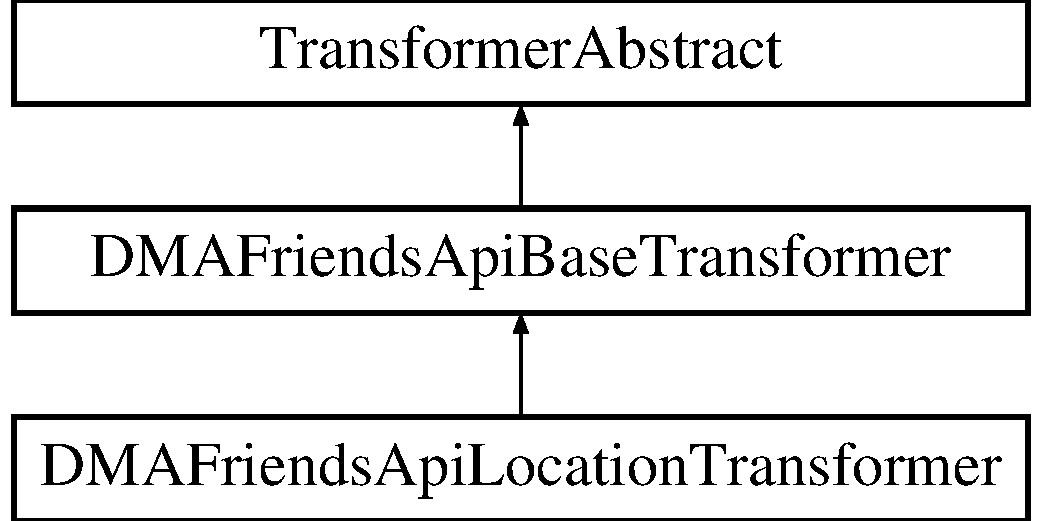
\includegraphics[height=3.000000cm]{d0/d5d/classDMA_1_1Friends_1_1Api_1_1LocationTransformer}
\end{center}
\end{figure}
\subsection*{Additional Inherited Members}


The documentation for this class was generated from the following file\+:\begin{DoxyCompactItemize}
\item 
api/Location\+Resource.\+php\end{DoxyCompactItemize}

\hypertarget{classDMA_1_1Friends_1_1Components_1_1Modal}{\section{D\+M\+A\textbackslash{}Friends\textbackslash{}Components\textbackslash{}Modal Class Reference}
\label{classDMA_1_1Friends_1_1Components_1_1Modal}\index{D\+M\+A\textbackslash{}\+Friends\textbackslash{}\+Components\textbackslash{}\+Modal@{D\+M\+A\textbackslash{}\+Friends\textbackslash{}\+Components\textbackslash{}\+Modal}}
}
Inheritance diagram for D\+M\+A\textbackslash{}Friends\textbackslash{}Components\textbackslash{}Modal\+:\begin{figure}[H]
\begin{center}
\leavevmode
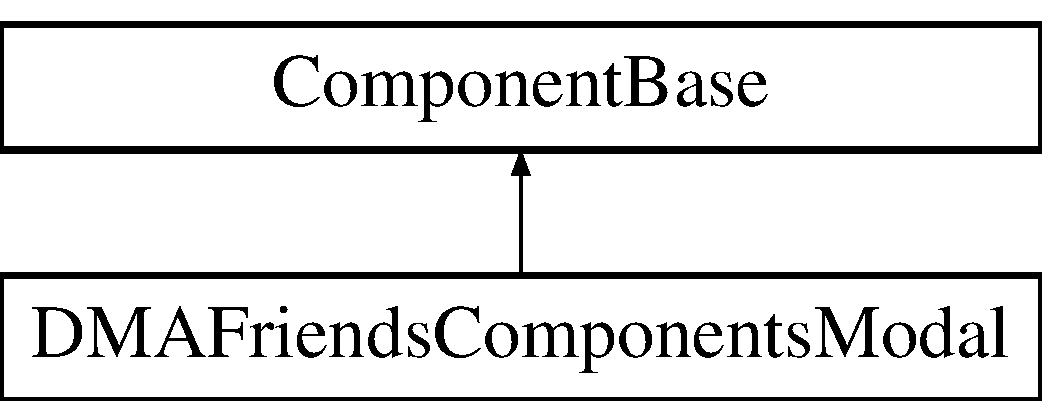
\includegraphics[height=2.000000cm]{df/da2/classDMA_1_1Friends_1_1Components_1_1Modal}
\end{center}
\end{figure}
\subsection*{Public Member Functions}
\begin{DoxyCompactItemize}
\item 
\hypertarget{classDMA_1_1Friends_1_1Components_1_1Modal_ad951492cf8acea02e0eaf24a029c0851}{{\bfseries component\+Details} ()}\label{classDMA_1_1Friends_1_1Components_1_1Modal_ad951492cf8acea02e0eaf24a029c0851}

\item 
\hypertarget{classDMA_1_1Friends_1_1Components_1_1Modal_aa109062a7350b8bd5dd168ede6aafd76}{{\bfseries define\+Properties} ()}\label{classDMA_1_1Friends_1_1Components_1_1Modal_aa109062a7350b8bd5dd168ede6aafd76}

\item 
\hypertarget{classDMA_1_1Friends_1_1Components_1_1Modal_ac8ccab598d85dc5339912bd627cd51a8}{{\bfseries on\+Render} ()}\label{classDMA_1_1Friends_1_1Components_1_1Modal_ac8ccab598d85dc5339912bd627cd51a8}

\item 
\hypertarget{classDMA_1_1Friends_1_1Components_1_1Modal_aed8e6b9a32f34a292d8a64619d483786}{{\bfseries on\+Run} ()}\label{classDMA_1_1Friends_1_1Components_1_1Modal_aed8e6b9a32f34a292d8a64619d483786}

\item 
\hypertarget{classDMA_1_1Friends_1_1Components_1_1Modal_a524d66800c7799a474a280e6fa77933c}{{\bfseries on\+Render\+Modal} ()}\label{classDMA_1_1Friends_1_1Components_1_1Modal_a524d66800c7799a474a280e6fa77933c}

\item 
\hyperlink{classDMA_1_1Friends_1_1Components_1_1Modal_a4e45e161a2624a34d59bf56294122ced}{make\+Partial} (\$partial, \$params=\mbox{[}$\,$\mbox{]}, \$throw\+Exception=true)
\end{DoxyCompactItemize}
\subsection*{Static Protected Member Functions}
\begin{DoxyCompactItemize}
\item 
static \hyperlink{classDMA_1_1Friends_1_1Components_1_1Modal_ac809c15fb0a9fc3b810afb9cc1d31ee8}{get\+Theme\+Partials\+Dir} ()
\end{DoxyCompactItemize}


\subsection{Member Function Documentation}
\hypertarget{classDMA_1_1Friends_1_1Components_1_1Modal_ac809c15fb0a9fc3b810afb9cc1d31ee8}{\index{D\+M\+A\+::\+Friends\+::\+Components\+::\+Modal@{D\+M\+A\+::\+Friends\+::\+Components\+::\+Modal}!get\+Theme\+Partials\+Dir@{get\+Theme\+Partials\+Dir}}
\index{get\+Theme\+Partials\+Dir@{get\+Theme\+Partials\+Dir}!D\+M\+A\+::\+Friends\+::\+Components\+::\+Modal@{D\+M\+A\+::\+Friends\+::\+Components\+::\+Modal}}
\subsubsection[{get\+Theme\+Partials\+Dir}]{\setlength{\rightskip}{0pt plus 5cm}static D\+M\+A\textbackslash{}\+Friends\textbackslash{}\+Components\textbackslash{}\+Modal\+::get\+Theme\+Partials\+Dir (
\begin{DoxyParamCaption}
{}
\end{DoxyParamCaption}
)\hspace{0.3cm}{\ttfamily [static]}, {\ttfamily [protected]}}}\label{classDMA_1_1Friends_1_1Components_1_1Modal_ac809c15fb0a9fc3b810afb9cc1d31ee8}
Get the path to the theme's partials

\begin{DoxyReturn}{Returns}
string \$path 
\end{DoxyReturn}

\begin{DoxyCode}
107     \{
108         $theme = Theme::getActiveTheme();
109         \textcolor{keywordflow}{return} $theme->getPath() . \textcolor{stringliteral}{'/partials/'};
110     \}
\end{DoxyCode}
\hypertarget{classDMA_1_1Friends_1_1Components_1_1Modal_a4e45e161a2624a34d59bf56294122ced}{\index{D\+M\+A\+::\+Friends\+::\+Components\+::\+Modal@{D\+M\+A\+::\+Friends\+::\+Components\+::\+Modal}!make\+Partial@{make\+Partial}}
\index{make\+Partial@{make\+Partial}!D\+M\+A\+::\+Friends\+::\+Components\+::\+Modal@{D\+M\+A\+::\+Friends\+::\+Components\+::\+Modal}}
\subsubsection[{make\+Partial}]{\setlength{\rightskip}{0pt plus 5cm}D\+M\+A\textbackslash{}\+Friends\textbackslash{}\+Components\textbackslash{}\+Modal\+::make\+Partial (
\begin{DoxyParamCaption}
\item[{}]{\$partial, }
\item[{}]{\$params = {\ttfamily \mbox{[}\mbox{]}}, }
\item[{}]{\$throw\+Exception = {\ttfamily true}}
\end{DoxyParamCaption}
)}}\label{classDMA_1_1Friends_1_1Components_1_1Modal_a4e45e161a2624a34d59bf56294122ced}
Implementation of View\+Maker-\/$>$make\+Partial that renders a partial in a modal dialog and can accept a partial from the active theme


\begin{DoxyParams}[1]{Parameters}
string & {\em \$partial} & Name of the partial to be rendered. The partial must reside in the active theme's \char`\"{}partials\char`\"{} directory\\
\hline
array & {\em \$params} & An array of parameters to be passed to make\+Partial. See Backend for details\\
\hline
boolean & {\em \$throw\+Exception} & if true an exception will be thrown if the partial is not available\\
\hline
\end{DoxyParams}
\begin{DoxyReturn}{Returns}
string \$content A rendered partial 
\end{DoxyReturn}

\begin{DoxyCode}
83     \{   
84         $partialsDir = self::getThemePartialsDir();
85         $partialPath = $partialsDir . $partial . \textcolor{stringliteral}{'.htm'};
86 
87         \textcolor{keywordflow}{if} (!File::isFile($partialPath)) \{
88             $partialPath = $this->getViewPath($partial) . \textcolor{stringliteral}{'.htm'};
89         \}
90 
91         \textcolor{keywordflow}{if} (!File::isFile($partialPath)) \{
92             \textcolor{keywordflow}{if} ($throwException)
93                 \textcolor{keywordflow}{throw} \textcolor{keyword}{new} \hyperlink{namespaceSystemException}{SystemException}(Lang::get(\textcolor{stringliteral}{'backend::lang.partial.not\_found'}, [\textcolor{stringliteral}{'
      name'} => $partialPath]));
94             \textcolor{keywordflow}{else}
95                 \textcolor{keywordflow}{return} \textcolor{keyword}{false};
96         \}   
97 
98         \textcolor{keywordflow}{return} $this->makeFileContents($partialPath, $params);
99     \}   
\end{DoxyCode}


The documentation for this class was generated from the following file\+:\begin{DoxyCompactItemize}
\item 
components/Modal.\+php\end{DoxyCompactItemize}

\hypertarget{classDMA_1_1Friends_1_1Plugin}{\section{D\-M\-A\textbackslash{}Friends\textbackslash{}Plugin Class Reference}
\label{classDMA_1_1Friends_1_1Plugin}\index{D\-M\-A\textbackslash{}\-Friends\textbackslash{}\-Plugin@{D\-M\-A\textbackslash{}\-Friends\textbackslash{}\-Plugin}}
}
Inheritance diagram for D\-M\-A\textbackslash{}Friends\textbackslash{}Plugin\-:\begin{figure}[H]
\begin{center}
\leavevmode
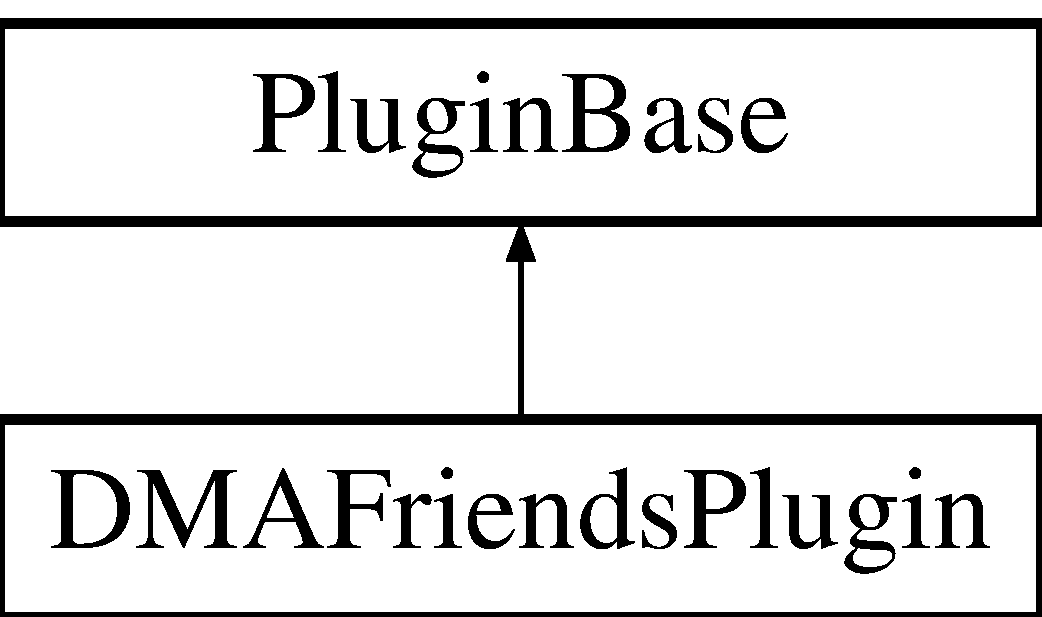
\includegraphics[height=2.000000cm]{db/d85/classDMA_1_1Friends_1_1Plugin}
\end{center}
\end{figure}
\subsection*{Public Member Functions}
\begin{DoxyCompactItemize}
\item 
\hyperlink{classDMA_1_1Friends_1_1Plugin_abcae4983c18bdb7b266c6aaa7a081d68}{plugin\-Details} ()
\item 
\hypertarget{classDMA_1_1Friends_1_1Plugin_a1f5f007ec6f0f3f16516cf1a2e19d296}{{\bfseries register\-Permissions} ()}\label{classDMA_1_1Friends_1_1Plugin_a1f5f007ec6f0f3f16516cf1a2e19d296}

\item 
\hypertarget{classDMA_1_1Friends_1_1Plugin_ad494274bdd3480e4623b5fec196352b3}{{\bfseries register\-Settings} ()}\label{classDMA_1_1Friends_1_1Plugin_ad494274bdd3480e4623b5fec196352b3}

\item 
\hypertarget{classDMA_1_1Friends_1_1Plugin_aaca6d71040b99d2151b2760c93f3e61c}{{\bfseries register\-Navigation} ()}\label{classDMA_1_1Friends_1_1Plugin_aaca6d71040b99d2151b2760c93f3e61c}

\item 
\hypertarget{classDMA_1_1Friends_1_1Plugin_aba0ea6e404e36aaba19174560d3781ac}{{\bfseries register\-Components} ()}\label{classDMA_1_1Friends_1_1Plugin_aba0ea6e404e36aaba19174560d3781ac}

\item 
\hyperlink{classDMA_1_1Friends_1_1Plugin_aee1fcfd6978df90e396e75223e24080a}{register\-Friends\-Activities} ()
\item 
\hypertarget{classDMA_1_1Friends_1_1Plugin_a8ff526c557ed7081a1f4c04194994305}{{\bfseries boot} ()}\label{classDMA_1_1Friends_1_1Plugin_a8ff526c557ed7081a1f4c04194994305}

\item 
\hypertarget{classDMA_1_1Friends_1_1Plugin_a900bf22951ffe9e109d1c14afdd261d5}{{\bfseries register\-Form\-Widgets} ()}\label{classDMA_1_1Friends_1_1Plugin_a900bf22951ffe9e109d1c14afdd261d5}

\item 
\hypertarget{classDMA_1_1Friends_1_1Plugin_adfd39323d7e2724cdacdb41d590b32e2}{{\bfseries register} ()}\label{classDMA_1_1Friends_1_1Plugin_adfd39323d7e2724cdacdb41d590b32e2}

\item 
\hypertarget{classDMA_1_1Friends_1_1Plugin_af4c0877dc0c5067f527fa414bc70de57}{{\bfseries register\-Report\-Widgets} ()}\label{classDMA_1_1Friends_1_1Plugin_af4c0877dc0c5067f527fa414bc70de57}

\item 
\hypertarget{classDMA_1_1Friends_1_1Plugin_aaab460ba502e3b45284785c291e39bf9}{{\bfseries register\-Mail\-Templates} ()}\label{classDMA_1_1Friends_1_1Plugin_aaab460ba502e3b45284785c291e39bf9}

\end{DoxyCompactItemize}
\subsection*{Public Attributes}
\begin{DoxyCompactItemize}
\item 
{\bfseries \$require}
\end{DoxyCompactItemize}


\subsection{Member Function Documentation}
\hypertarget{classDMA_1_1Friends_1_1Plugin_abcae4983c18bdb7b266c6aaa7a081d68}{\index{D\-M\-A\-::\-Friends\-::\-Plugin@{D\-M\-A\-::\-Friends\-::\-Plugin}!plugin\-Details@{plugin\-Details}}
\index{plugin\-Details@{plugin\-Details}!DMA::Friends::Plugin@{D\-M\-A\-::\-Friends\-::\-Plugin}}
\subsubsection[{plugin\-Details}]{\setlength{\rightskip}{0pt plus 5cm}D\-M\-A\textbackslash{}\-Friends\textbackslash{}\-Plugin\-::plugin\-Details (
\begin{DoxyParamCaption}
{}
\end{DoxyParamCaption}
)}}\label{classDMA_1_1Friends_1_1Plugin_abcae4983c18bdb7b266c6aaa7a081d68}
Returns information about this plugin.

\begin{DoxyReturn}{Returns}
array 
\end{DoxyReturn}

\begin{DoxyCode}
37     \{
38         \textcolor{keywordflow}{return} [
39             \textcolor{stringliteral}{'name'}        => \textcolor{stringliteral}{'Friends'},
40             \textcolor{stringliteral}{'description'} => \textcolor{stringliteral}{'A platform for users to earn badges and redeem rewards'},
41             \textcolor{stringliteral}{'author'}      => \textcolor{stringliteral}{'Dallas Museum of Art'},
42             \textcolor{stringliteral}{'icon'}        => \textcolor{stringliteral}{'icon-leaf'}
43         ];
44     \}
\end{DoxyCode}
\hypertarget{classDMA_1_1Friends_1_1Plugin_aee1fcfd6978df90e396e75223e24080a}{\index{D\-M\-A\-::\-Friends\-::\-Plugin@{D\-M\-A\-::\-Friends\-::\-Plugin}!register\-Friends\-Activities@{register\-Friends\-Activities}}
\index{register\-Friends\-Activities@{register\-Friends\-Activities}!DMA::Friends::Plugin@{D\-M\-A\-::\-Friends\-::\-Plugin}}
\subsubsection[{register\-Friends\-Activities}]{\setlength{\rightskip}{0pt plus 5cm}D\-M\-A\textbackslash{}\-Friends\textbackslash{}\-Plugin\-::register\-Friends\-Activities (
\begin{DoxyParamCaption}
{}
\end{DoxyParamCaption}
)}}\label{classDMA_1_1Friends_1_1Plugin_aee1fcfd6978df90e396e75223e24080a}
Register additional friends activity types 
\begin{DoxyCode}
147     \{
148         \textcolor{keywordflow}{return} [
149             \textcolor{stringliteral}{'DMA\(\backslash\)Friends\(\backslash\)Activities\(\backslash\)ActivityCode'}   => \textcolor{stringliteral}{'ActivityCode'},
150             \textcolor{stringliteral}{'DMA\(\backslash\)Friends\(\backslash\)Activities\(\backslash\)LikeWorkOfArt'}  => \textcolor{stringliteral}{'LikeWorkOfArt'},
151         ];
152     \}
\end{DoxyCode}


\subsection{Member Data Documentation}
\hypertarget{classDMA_1_1Friends_1_1Plugin_a3c98aaa659a7b26aaef32d2767f14738}{\index{D\-M\-A\-::\-Friends\-::\-Plugin@{D\-M\-A\-::\-Friends\-::\-Plugin}!\$require@{\$require}}
\index{\$require@{\$require}!DMA::Friends::Plugin@{D\-M\-A\-::\-Friends\-::\-Plugin}}
\subsubsection[{\$require}]{\setlength{\rightskip}{0pt plus 5cm}D\-M\-A\textbackslash{}\-Friends\textbackslash{}\-Plugin\-::\$require}}\label{classDMA_1_1Friends_1_1Plugin_a3c98aaa659a7b26aaef32d2767f14738}
{\bfseries Initial value\-:}
\begin{DoxyCode}
= [
        \textcolor{stringliteral}{'RainLab.User'}
    ]
\end{DoxyCode}


The documentation for this class was generated from the following file\-:\begin{DoxyCompactItemize}
\item 
Plugin.\-php\end{DoxyCompactItemize}

\hypertarget{classDMA_1_1Friends_1_1Wordpress_1_1Post}{\section{D\-M\-A\textbackslash{}Friends\textbackslash{}Wordpress\textbackslash{}Post Class Reference}
\label{classDMA_1_1Friends_1_1Wordpress_1_1Post}\index{D\-M\-A\textbackslash{}\-Friends\textbackslash{}\-Wordpress\textbackslash{}\-Post@{D\-M\-A\textbackslash{}\-Friends\textbackslash{}\-Wordpress\textbackslash{}\-Post}}
}
Inheritance diagram for D\-M\-A\textbackslash{}Friends\textbackslash{}Wordpress\textbackslash{}Post\-:\begin{figure}[H]
\begin{center}
\leavevmode
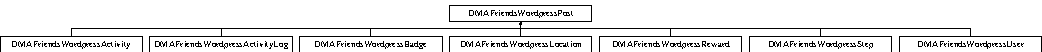
\includegraphics[height=9.000000cm]{d2/de2/classDMA_1_1Friends_1_1Wordpress_1_1Post}
\end{center}
\end{figure}
\subsection*{Public Member Functions}
\begin{DoxyCompactItemize}
\item 
\hyperlink{classDMA_1_1Friends_1_1Wordpress_1_1Post_a4eb2c6b3e89a43b3221e9e2564059510}{import} (\$limit=0)
\item 
\hyperlink{classDMA_1_1Friends_1_1Wordpress_1_1Post_adb1c6652d06b360d1f81d14dde95b5b1}{merge\-Metadata} (\&\$post)
\item 
\hyperlink{classDMA_1_1Friends_1_1Wordpress_1_1Post_af6960d9c63c4224f6f481c88d2b5d076}{epoch\-To\-Timestamp} (\$val)
\end{DoxyCompactItemize}
\subsection*{Public Attributes}
\begin{DoxyCompactItemize}
\item 
\hyperlink{classDMA_1_1Friends_1_1Wordpress_1_1Post_a38fc35f2a6a04046e386cfd3f3564d89}{\$schema}
\item 
\hyperlink{classDMA_1_1Friends_1_1Wordpress_1_1Post_a9b0ea251e8ba6b7161fc51ffa8fb72d8}{\$post\-Type} = null
\item 
\hyperlink{classDMA_1_1Friends_1_1Wordpress_1_1Post_a8a3df2e9db7f90d348d27ea9354176b1}{\$model} = null
\end{DoxyCompactItemize}
\subsection*{Protected Member Functions}
\begin{DoxyCompactItemize}
\item 
\hyperlink{classDMA_1_1Friends_1_1Wordpress_1_1Post_a8969b8476b3ba0afc871532f6f936514}{convert\-Values} (\$key, \$val)
\item 
\hyperlink{classDMA_1_1Friends_1_1Wordpress_1_1Post_a37fb0931dadba67a39a637b336787663}{real\-Boolean} (\$val)
\item 
\hyperlink{classDMA_1_1Friends_1_1Wordpress_1_1Post_a5fbf4b003c2136d8497ddd7d726ad671}{real\-Time\-Restriction} (\$val)
\item 
\hyperlink{classDMA_1_1Friends_1_1Wordpress_1_1Post_a427b14dd99893217929ee8ee93977628}{convert\-Time\-Restricted\-Data} (\$data)
\end{DoxyCompactItemize}
\subsection*{Protected Attributes}
\begin{DoxyCompactItemize}
\item 
\hyperlink{classDMA_1_1Friends_1_1Wordpress_1_1Post_ac0b74792fa83b0a9dafda52eec451e50}{\$restricted\-Times}
\item 
\hyperlink{classDMA_1_1Friends_1_1Wordpress_1_1Post_ac9f76efeb858c94d5ab78e74b4301c16}{\$exclude\-Fields} = \mbox{[}$\,$\mbox{]}
\end{DoxyCompactItemize}


\subsection{Detailed Description}
Abstract class for importing/exporting wordpress posts to and from laravel models 

\subsection{Member Function Documentation}
\hypertarget{classDMA_1_1Friends_1_1Wordpress_1_1Post_a427b14dd99893217929ee8ee93977628}{\index{D\-M\-A\-::\-Friends\-::\-Wordpress\-::\-Post@{D\-M\-A\-::\-Friends\-::\-Wordpress\-::\-Post}!convert\-Time\-Restricted\-Data@{convert\-Time\-Restricted\-Data}}
\index{convert\-Time\-Restricted\-Data@{convert\-Time\-Restricted\-Data}!DMA::Friends::Wordpress::Post@{D\-M\-A\-::\-Friends\-::\-Wordpress\-::\-Post}}
\subsubsection[{convert\-Time\-Restricted\-Data}]{\setlength{\rightskip}{0pt plus 5cm}D\-M\-A\textbackslash{}\-Friends\textbackslash{}\-Wordpress\textbackslash{}\-Post\-::convert\-Time\-Restricted\-Data (
\begin{DoxyParamCaption}
\item[{}]{\$data}
\end{DoxyParamCaption}
)\hspace{0.3cm}{\ttfamily [protected]}}}\label{classDMA_1_1Friends_1_1Wordpress_1_1Post_a427b14dd99893217929ee8ee93977628}
Converts \char`\"{}time restricted\char`\"{} data settings for activities into a serialized field of configuration settings


\begin{DoxyParams}[1]{Parameters}
array & {\em \$data} & \\
\hline
\end{DoxyParams}
\begin{DoxyReturn}{Returns}
\$data A serialized version of the processed data 
\end{DoxyReturn}

\begin{DoxyCode}
296     \{
297         $d = [
298             \textcolor{stringliteral}{'start\_time'}    => null,
299             \textcolor{stringliteral}{'end\_time'}      => null,
300             \textcolor{stringliteral}{'days'}          => [
301                 1   => \textcolor{keyword}{false},
302                 2   => \textcolor{keyword}{false},
303                 3   => \textcolor{keyword}{false},
304                 4   => \textcolor{keyword}{false},
305                 5   => \textcolor{keyword}{false},
306                 6   => \textcolor{keyword}{false},
307                 7   => \textcolor{keyword}{false},
308             ]
309         ];
310 
311         \textcolor{keywordflow}{foreach}($data as $val) \{
312             list($k, $v) = explode(\textcolor{charliteral}{'|'}, $val);
313             
314             \textcolor{keywordflow}{switch}($k) \{
315                 \textcolor{keywordflow}{case} \textcolor{stringliteral}{'\_badgeos\_time\_restriction\_hour\_begin'}:
316                     $d[\textcolor{stringliteral}{'start\_time'}] = $v;
317                     \textcolor{keywordflow}{break}; 
318                 \textcolor{keywordflow}{case} \textcolor{stringliteral}{'\_badgeos\_time\_restriction\_hour\_end'}:
319                     $d[\textcolor{stringliteral}{'end\_time'}] = $v;
320                     \textcolor{keywordflow}{break}; 
321                 \textcolor{keywordflow}{case} \textcolor{stringliteral}{'\_badgeos\_time\_restriction\_days'}:
322                     $d[\textcolor{stringliteral}{'days'}][date(\textcolor{charliteral}{'N'}, strtotime($v))] = \textcolor{keyword}{true};
323                     \textcolor{keywordflow}{break};
324             \}    
325         \}
326 
327         \textcolor{keywordflow}{return} serialize($d);
328 
329     \}
\end{DoxyCode}
\hypertarget{classDMA_1_1Friends_1_1Wordpress_1_1Post_a8969b8476b3ba0afc871532f6f936514}{\index{D\-M\-A\-::\-Friends\-::\-Wordpress\-::\-Post@{D\-M\-A\-::\-Friends\-::\-Wordpress\-::\-Post}!convert\-Values@{convert\-Values}}
\index{convert\-Values@{convert\-Values}!DMA::Friends::Wordpress::Post@{D\-M\-A\-::\-Friends\-::\-Wordpress\-::\-Post}}
\subsubsection[{convert\-Values}]{\setlength{\rightskip}{0pt plus 5cm}D\-M\-A\textbackslash{}\-Friends\textbackslash{}\-Wordpress\textbackslash{}\-Post\-::convert\-Values (
\begin{DoxyParamCaption}
\item[{}]{\$key, }
\item[{}]{\$val}
\end{DoxyParamCaption}
)\hspace{0.3cm}{\ttfamily [protected]}}}\label{classDMA_1_1Friends_1_1Wordpress_1_1Post_a8969b8476b3ba0afc871532f6f936514}
Converts special fields to the appropriate value type


\begin{DoxyParams}{Parameters}
{\em \$key} & \\
\hline
{\em \$val} & \\
\hline
\end{DoxyParams}
\begin{DoxyReturn}{Returns}
\$val The converted value 
\end{DoxyReturn}

\begin{DoxyCode}
204     \{
205         \textcolor{comment}{// Fields that start with is\_ are booleans}
206         \textcolor{comment}{// And need to be reformated to a real boolean field}
207         \textcolor{keywordflow}{if} (substr($key, 0, 3) == \textcolor{stringliteral}{'is\_'}) \{
208             $val = $this->\hyperlink{classDMA_1_1Friends_1_1Wordpress_1_1Post_a37fb0931dadba67a39a637b336787663}{realBoolean}($val);
209         \}   
210 
211         \textcolor{keywordflow}{switch}($key) \{
212             \textcolor{keywordflow}{case} \textcolor{stringliteral}{'time\_restriction'}:
213                 $val = $this->\hyperlink{classDMA_1_1Friends_1_1Wordpress_1_1Post_a5fbf4b003c2136d8497ddd7d726ad671}{realTimeRestriction}($val);
214                 \textcolor{keywordflow}{break};
215             \textcolor{keywordflow}{case} \textcolor{stringliteral}{'date\_begin'}:
216             \textcolor{keywordflow}{case} \textcolor{stringliteral}{'date\_end'}:
217                 \textcolor{keywordflow}{if} (!is\_numeric($val)) \{
218                     $val = strtotime($val);
219                 \}
220                 $val = $this->\hyperlink{classDMA_1_1Friends_1_1Wordpress_1_1Post_af6960d9c63c4224f6f481c88d2b5d076}{epochToTimestamp}($val);
221                 \textcolor{keywordflow}{break};
222         \}
223 
224         \textcolor{keywordflow}{return} $val;
225     \}
\end{DoxyCode}
\hypertarget{classDMA_1_1Friends_1_1Wordpress_1_1Post_af6960d9c63c4224f6f481c88d2b5d076}{\index{D\-M\-A\-::\-Friends\-::\-Wordpress\-::\-Post@{D\-M\-A\-::\-Friends\-::\-Wordpress\-::\-Post}!epoch\-To\-Timestamp@{epoch\-To\-Timestamp}}
\index{epoch\-To\-Timestamp@{epoch\-To\-Timestamp}!DMA::Friends::Wordpress::Post@{D\-M\-A\-::\-Friends\-::\-Wordpress\-::\-Post}}
\subsubsection[{epoch\-To\-Timestamp}]{\setlength{\rightskip}{0pt plus 5cm}D\-M\-A\textbackslash{}\-Friends\textbackslash{}\-Wordpress\textbackslash{}\-Post\-::epoch\-To\-Timestamp (
\begin{DoxyParamCaption}
\item[{}]{\$val}
\end{DoxyParamCaption}
)}}\label{classDMA_1_1Friends_1_1Wordpress_1_1Post_af6960d9c63c4224f6f481c88d2b5d076}
Convert an epoch value to the appropriate timestamp


\begin{DoxyParams}{Parameters}
{\em \$val} & \\
\hline
\end{DoxyParams}
\begin{DoxyReturn}{Returns}
\$timestamp 
\end{DoxyReturn}

\begin{DoxyCode}
282     \{
283         \textcolor{keywordflow}{return} date(\textcolor{stringliteral}{'Y-m-d H:i:s'}, $val);
284     \}
\end{DoxyCode}
\hypertarget{classDMA_1_1Friends_1_1Wordpress_1_1Post_a4eb2c6b3e89a43b3221e9e2564059510}{\index{D\-M\-A\-::\-Friends\-::\-Wordpress\-::\-Post@{D\-M\-A\-::\-Friends\-::\-Wordpress\-::\-Post}!import@{import}}
\index{import@{import}!DMA::Friends::Wordpress::Post@{D\-M\-A\-::\-Friends\-::\-Wordpress\-::\-Post}}
\subsubsection[{import}]{\setlength{\rightskip}{0pt plus 5cm}D\-M\-A\textbackslash{}\-Friends\textbackslash{}\-Wordpress\textbackslash{}\-Post\-::import (
\begin{DoxyParamCaption}
\item[{}]{\$limit = {\ttfamily 0}}
\end{DoxyParamCaption}
)}}\label{classDMA_1_1Friends_1_1Wordpress_1_1Post_a4eb2c6b3e89a43b3221e9e2564059510}
Imports a wordpress post as an elequent model


\begin{DoxyParams}[1]{Parameters}
int & {\em \$limit} & The number of records to import at once\\
\hline
\end{DoxyParams}
\begin{DoxyReturn}{Returns}
\$count The number of records that have been imported 
\end{DoxyReturn}

\begin{DoxyCode}
133     \{
134         $count  = 0;
135         $id     = (int)DB::table($this->model->table)->max(\textcolor{stringliteral}{'wordpress\_id'});
136 
137         $posts = $this->db->table(\textcolor{stringliteral}{'wp\_posts'})
138             ->where(\textcolor{stringliteral}{'ID'}, \textcolor{charliteral}{'>'}, $id)
139             ->where(\textcolor{stringliteral}{'post\_type'}, $this->postType)
140             ->get();
141 
142         \textcolor{keywordflow}{foreach}($posts as $post) \{
143             $this->\hyperlink{classDMA_1_1Friends_1_1Wordpress_1_1Post_adb1c6652d06b360d1f81d14dde95b5b1}{mergeMetadata}($post);
144 
145             \hyperlink{classDMA_1_1Friends_1_1Wordpress_1_1Post_a8a3df2e9db7f90d348d27ea9354176b1}{$model} = \textcolor{keyword}{new} \hyperlink{classDMA_1_1Friends_1_1Wordpress_1_1Post_a8a3df2e9db7f90d348d27ea9354176b1}{$this->model};
146 
147             \textcolor{keywordflow}{foreach}((array)$post as $key => $val) \{
148                 \textcolor{keywordflow}{if} (in\_array($key, $this->excludeFields)) \textcolor{keywordflow}{continue};
149 
150                 \textcolor{keywordflow}{if} (isset($this->schema[$key])) \{
151                     $val = $this->\hyperlink{classDMA_1_1Friends_1_1Wordpress_1_1Post_a8969b8476b3ba0afc871532f6f936514}{convertValues}($this->schema[$key], $val);
152 
153                     \textcolor{keywordflow}{if} (!in\_array($this->schema[$key], $this->restrictedTimes)) \{
154                         \hyperlink{classDMA_1_1Friends_1_1Wordpress_1_1Post_a8a3df2e9db7f90d348d27ea9354176b1}{$model}->\{$this->schema[$key]\} = $val;
155                     \}
156                 \} elseif ($key == \textcolor{stringliteral}{'time\_restriction\_data'}) \{
157                     \hyperlink{classDMA_1_1Friends_1_1Wordpress_1_1Post_a8a3df2e9db7f90d348d27ea9354176b1}{$model}->time\_restriction\_data = $this->
      \hyperlink{classDMA_1_1Friends_1_1Wordpress_1_1Post_a427b14dd99893217929ee8ee93977628}{convertTimeRestrictedData}($post->\{$key\});
158                 \}
159 
160             \}
161 
162             \textcolor{keywordflow}{if} (\hyperlink{classDMA_1_1Friends_1_1Wordpress_1_1Post_a8a3df2e9db7f90d348d27ea9354176b1}{$model}->forceSave()) \{
163                 $count++;
164             \}
165         \}
166 
167         \textcolor{keywordflow}{return} $count;
168 
169     \}
\end{DoxyCode}
\hypertarget{classDMA_1_1Friends_1_1Wordpress_1_1Post_adb1c6652d06b360d1f81d14dde95b5b1}{\index{D\-M\-A\-::\-Friends\-::\-Wordpress\-::\-Post@{D\-M\-A\-::\-Friends\-::\-Wordpress\-::\-Post}!merge\-Metadata@{merge\-Metadata}}
\index{merge\-Metadata@{merge\-Metadata}!DMA::Friends::Wordpress::Post@{D\-M\-A\-::\-Friends\-::\-Wordpress\-::\-Post}}
\subsubsection[{merge\-Metadata}]{\setlength{\rightskip}{0pt plus 5cm}D\-M\-A\textbackslash{}\-Friends\textbackslash{}\-Wordpress\textbackslash{}\-Post\-::merge\-Metadata (
\begin{DoxyParamCaption}
\item[{\&}]{\$post}
\end{DoxyParamCaption}
)}}\label{classDMA_1_1Friends_1_1Wordpress_1_1Post_adb1c6652d06b360d1f81d14dde95b5b1}
Merge wordpress metadata with the original post


\begin{DoxyParams}{Parameters}
{\em \$post} & A wordpress post object \\
\hline
\end{DoxyParams}

\begin{DoxyCode}
178     \{
179         $metadata = $this->db->table(\textcolor{stringliteral}{'wp\_postmeta'})
180             ->where(\textcolor{stringliteral}{'post\_id'}, $post->ID)
181             ->get();
182 
183         \textcolor{keywordflow}{foreach}($metadata as $meta) \{
184             \textcolor{keywordflow}{if} (in\_array($meta->meta\_key, $this->restrictedTimes)) \{
185                 \textcolor{comment}{// For now we will save as a meta:key combo.  The data will be sorted later in processing}
186                 $post->time\_restriction\_data[] = $meta->meta\_key . \textcolor{charliteral}{'|'} . $meta->meta\_value;
187             \} \textcolor{keywordflow}{else} \{
188                 $post->\{$meta->meta\_key\} = $meta->meta\_value;
189             \}
190         \}
191 
192     \}
\end{DoxyCode}
\hypertarget{classDMA_1_1Friends_1_1Wordpress_1_1Post_a37fb0931dadba67a39a637b336787663}{\index{D\-M\-A\-::\-Friends\-::\-Wordpress\-::\-Post@{D\-M\-A\-::\-Friends\-::\-Wordpress\-::\-Post}!real\-Boolean@{real\-Boolean}}
\index{real\-Boolean@{real\-Boolean}!DMA::Friends::Wordpress::Post@{D\-M\-A\-::\-Friends\-::\-Wordpress\-::\-Post}}
\subsubsection[{real\-Boolean}]{\setlength{\rightskip}{0pt plus 5cm}D\-M\-A\textbackslash{}\-Friends\textbackslash{}\-Wordpress\textbackslash{}\-Post\-::real\-Boolean (
\begin{DoxyParamCaption}
\item[{}]{\$val}
\end{DoxyParamCaption}
)\hspace{0.3cm}{\ttfamily [protected]}}}\label{classDMA_1_1Friends_1_1Wordpress_1_1Post_a37fb0931dadba67a39a637b336787663}
convert wordpress' infinite possibility of boolean values into a real boolean value


\begin{DoxyParams}{Parameters}
{\em \$val} & \\
\hline
\end{DoxyParams}
\begin{DoxyReturn}{Returns}
\$val 
\end{DoxyReturn}

\begin{DoxyCode}
235     \{
236         $val = strtolower($val);
237 
238         \textcolor{keywordflow}{switch}($val) \{
239             \textcolor{keywordflow}{case} \textcolor{stringliteral}{'yes'}:
240             \textcolor{keywordflow}{case} \textcolor{stringliteral}{'hidden'}:
241             \textcolor{keywordflow}{case} \textcolor{stringliteral}{'publish'}:
242                 $val = \textcolor{keyword}{true};
243                 \textcolor{keywordflow}{break};
244             \textcolor{keywordflow}{case} \textcolor{stringliteral}{'no'}:
245             \textcolor{keywordflow}{case} \textcolor{stringliteral}{'show'}:
246             \textcolor{keywordflow}{case} \textcolor{stringliteral}{'draft'}:
247                 $val = \textcolor{keyword}{false};
248                 \textcolor{keywordflow}{break};
249         \}
250 
251         \textcolor{keywordflow}{return} $val;
252     \}
\end{DoxyCode}
\hypertarget{classDMA_1_1Friends_1_1Wordpress_1_1Post_a5fbf4b003c2136d8497ddd7d726ad671}{\index{D\-M\-A\-::\-Friends\-::\-Wordpress\-::\-Post@{D\-M\-A\-::\-Friends\-::\-Wordpress\-::\-Post}!real\-Time\-Restriction@{real\-Time\-Restriction}}
\index{real\-Time\-Restriction@{real\-Time\-Restriction}!DMA::Friends::Wordpress::Post@{D\-M\-A\-::\-Friends\-::\-Wordpress\-::\-Post}}
\subsubsection[{real\-Time\-Restriction}]{\setlength{\rightskip}{0pt plus 5cm}D\-M\-A\textbackslash{}\-Friends\textbackslash{}\-Wordpress\textbackslash{}\-Post\-::real\-Time\-Restriction (
\begin{DoxyParamCaption}
\item[{}]{\$val}
\end{DoxyParamCaption}
)\hspace{0.3cm}{\ttfamily [protected]}}}\label{classDMA_1_1Friends_1_1Wordpress_1_1Post_a5fbf4b003c2136d8497ddd7d726ad671}
Convert a time restriction into the appropriate constant


\begin{DoxyParams}{Parameters}
{\em \$val} & \\
\hline
\end{DoxyParams}
\begin{DoxyReturn}{Returns}
\$val 
\end{DoxyReturn}

\begin{DoxyCode}
262     \{
263         \textcolor{keywordflow}{if} ($val == \textcolor{stringliteral}{'hours'}) \{
264             $val = \hyperlink{classDMA_1_1Friends_1_1Models_1_1Activity_ac78040e8784e02c2d1bcce5221ac6cb8}{Activity::TIME\_RESTRICT\_HOURS};
265         \} \textcolor{keywordflow}{else} \textcolor{keywordflow}{if} ($val == \textcolor{stringliteral}{'days'}) \{
266             $val = \hyperlink{classDMA_1_1Friends_1_1Models_1_1Activity_a71b85478f20cda144aeffe010364a0f7}{Activity::TIME\_RESTRICT\_DAYS};
267         \} \textcolor{keywordflow}{else} \{
268             $val = \hyperlink{classDMA_1_1Friends_1_1Models_1_1Activity_ab9dd8b18c4810beabdcf8e45039913c8}{Activity::TIME\_RESTRICT\_NONE};
269         \}
270 
271         \textcolor{keywordflow}{return} $val;
272     \}
\end{DoxyCode}


\subsection{Member Data Documentation}
\hypertarget{classDMA_1_1Friends_1_1Wordpress_1_1Post_ac9f76efeb858c94d5ab78e74b4301c16}{\index{D\-M\-A\-::\-Friends\-::\-Wordpress\-::\-Post@{D\-M\-A\-::\-Friends\-::\-Wordpress\-::\-Post}!\$exclude\-Fields@{\$exclude\-Fields}}
\index{\$exclude\-Fields@{\$exclude\-Fields}!DMA::Friends::Wordpress::Post@{D\-M\-A\-::\-Friends\-::\-Wordpress\-::\-Post}}
\subsubsection[{\$exclude\-Fields}]{\setlength{\rightskip}{0pt plus 5cm}D\-M\-A\textbackslash{}\-Friends\textbackslash{}\-Wordpress\textbackslash{}\-Post\-::\$exclude\-Fields = \mbox{[}$\,$\mbox{]}\hspace{0.3cm}{\ttfamily [protected]}}}\label{classDMA_1_1Friends_1_1Wordpress_1_1Post_ac9f76efeb858c94d5ab78e74b4301c16}
Exclude fields from being imported \hypertarget{classDMA_1_1Friends_1_1Wordpress_1_1Post_a8a3df2e9db7f90d348d27ea9354176b1}{\index{D\-M\-A\-::\-Friends\-::\-Wordpress\-::\-Post@{D\-M\-A\-::\-Friends\-::\-Wordpress\-::\-Post}!\$model@{\$model}}
\index{\$model@{\$model}!DMA::Friends::Wordpress::Post@{D\-M\-A\-::\-Friends\-::\-Wordpress\-::\-Post}}
\subsubsection[{\$model}]{\setlength{\rightskip}{0pt plus 5cm}D\-M\-A\textbackslash{}\-Friends\textbackslash{}\-Wordpress\textbackslash{}\-Post\-::\$model = null}}\label{classDMA_1_1Friends_1_1Wordpress_1_1Post_a8a3df2e9db7f90d348d27ea9354176b1}
A laravel model to represent the data \hypertarget{classDMA_1_1Friends_1_1Wordpress_1_1Post_a9b0ea251e8ba6b7161fc51ffa8fb72d8}{\index{D\-M\-A\-::\-Friends\-::\-Wordpress\-::\-Post@{D\-M\-A\-::\-Friends\-::\-Wordpress\-::\-Post}!\$post\-Type@{\$post\-Type}}
\index{\$post\-Type@{\$post\-Type}!DMA::Friends::Wordpress::Post@{D\-M\-A\-::\-Friends\-::\-Wordpress\-::\-Post}}
\subsubsection[{\$post\-Type}]{\setlength{\rightskip}{0pt plus 5cm}D\-M\-A\textbackslash{}\-Friends\textbackslash{}\-Wordpress\textbackslash{}\-Post\-::\$post\-Type = null}}\label{classDMA_1_1Friends_1_1Wordpress_1_1Post_a9b0ea251e8ba6b7161fc51ffa8fb72d8}
\hyperlink{classDMA_1_1Friends_1_1Wordpress_1_1Post}{Post} type in wordpress \hypertarget{classDMA_1_1Friends_1_1Wordpress_1_1Post_ac0b74792fa83b0a9dafda52eec451e50}{\index{D\-M\-A\-::\-Friends\-::\-Wordpress\-::\-Post@{D\-M\-A\-::\-Friends\-::\-Wordpress\-::\-Post}!\$restricted\-Times@{\$restricted\-Times}}
\index{\$restricted\-Times@{\$restricted\-Times}!DMA::Friends::Wordpress::Post@{D\-M\-A\-::\-Friends\-::\-Wordpress\-::\-Post}}
\subsubsection[{\$restricted\-Times}]{\setlength{\rightskip}{0pt plus 5cm}D\-M\-A\textbackslash{}\-Friends\textbackslash{}\-Wordpress\textbackslash{}\-Post\-::\$restricted\-Times\hspace{0.3cm}{\ttfamily [protected]}}}\label{classDMA_1_1Friends_1_1Wordpress_1_1Post_ac0b74792fa83b0a9dafda52eec451e50}
{\bfseries Initial value\-:}
\begin{DoxyCode}
= [
        \textcolor{stringliteral}{'\_badgeos\_time\_restriction\_days'},
        \textcolor{stringliteral}{'\_badgeos\_time\_restriction\_hour\_begin'},
        \textcolor{stringliteral}{'\_badgeos\_time\_restriction\_hour\_end'}
    ]
\end{DoxyCode}
Handle special settings fields for restricted hours and dates \hypertarget{classDMA_1_1Friends_1_1Wordpress_1_1Post_a38fc35f2a6a04046e386cfd3f3564d89}{\index{D\-M\-A\-::\-Friends\-::\-Wordpress\-::\-Post@{D\-M\-A\-::\-Friends\-::\-Wordpress\-::\-Post}!\$schema@{\$schema}}
\index{\$schema@{\$schema}!DMA::Friends::Wordpress::Post@{D\-M\-A\-::\-Friends\-::\-Wordpress\-::\-Post}}
\subsubsection[{\$schema}]{\setlength{\rightskip}{0pt plus 5cm}D\-M\-A\textbackslash{}\-Friends\textbackslash{}\-Wordpress\textbackslash{}\-Post\-::\$schema}}\label{classDMA_1_1Friends_1_1Wordpress_1_1Post_a38fc35f2a6a04046e386cfd3f3564d89}
{\bfseries Initial value\-:}
\begin{DoxyCode}
= [
        
        \textcolor{stringliteral}{'ID'}                                            => \textcolor{stringliteral}{'wordpress\_id'}
\end{DoxyCode}
array The schema defines the mapping between wordpress and laravel. With the key being the wordpress key, and the value being the Laravel key 

The documentation for this class was generated from the following file\-:\begin{DoxyCompactItemize}
\item 
wordpress/Post.\-php\end{DoxyCompactItemize}

\hypertarget{classDMA_1_1Friends_1_1FormWidgets_1_1RequiredSteps}{\section{D\-M\-A\textbackslash{}Friends\textbackslash{}Form\-Widgets\textbackslash{}Required\-Steps Class Reference}
\label{classDMA_1_1Friends_1_1FormWidgets_1_1RequiredSteps}\index{D\-M\-A\textbackslash{}\-Friends\textbackslash{}\-Form\-Widgets\textbackslash{}\-Required\-Steps@{D\-M\-A\textbackslash{}\-Friends\textbackslash{}\-Form\-Widgets\textbackslash{}\-Required\-Steps}}
}
Inheritance diagram for D\-M\-A\textbackslash{}Friends\textbackslash{}Form\-Widgets\textbackslash{}Required\-Steps\-:\begin{figure}[H]
\begin{center}
\leavevmode
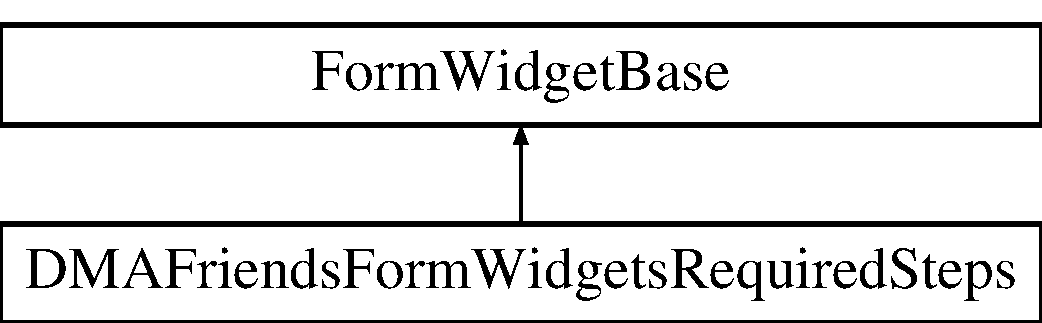
\includegraphics[height=2.000000cm]{dd/db5/classDMA_1_1Friends_1_1FormWidgets_1_1RequiredSteps}
\end{center}
\end{figure}
\subsection*{Public Member Functions}
\begin{DoxyCompactItemize}
\item 
\hypertarget{classDMA_1_1Friends_1_1FormWidgets_1_1RequiredSteps_a7515c39fb1cd2bf16604b907e98485e2}{{\bfseries widget\-Details} ()}\label{classDMA_1_1Friends_1_1FormWidgets_1_1RequiredSteps_a7515c39fb1cd2bf16604b907e98485e2}

\item 
\hypertarget{classDMA_1_1Friends_1_1FormWidgets_1_1RequiredSteps_ae3ebaf8a7cf65ac562796d7bd3bc4567}{{\bfseries render} ()}\label{classDMA_1_1Friends_1_1FormWidgets_1_1RequiredSteps_ae3ebaf8a7cf65ac562796d7bd3bc4567}

\end{DoxyCompactItemize}


The documentation for this class was generated from the following file\-:\begin{DoxyCompactItemize}
\item 
formwidgets/Required\-Steps.\-php\end{DoxyCompactItemize}

\hypertarget{classDMA_1_1Friends_1_1Wordpress_1_1Reward}{\section{D\-M\-A\textbackslash{}Friends\textbackslash{}Wordpress\textbackslash{}Reward Class Reference}
\label{classDMA_1_1Friends_1_1Wordpress_1_1Reward}\index{D\-M\-A\textbackslash{}\-Friends\textbackslash{}\-Wordpress\textbackslash{}\-Reward@{D\-M\-A\textbackslash{}\-Friends\textbackslash{}\-Wordpress\textbackslash{}\-Reward}}
}
Inheritance diagram for D\-M\-A\textbackslash{}Friends\textbackslash{}Wordpress\textbackslash{}Reward\-:\begin{figure}[H]
\begin{center}
\leavevmode
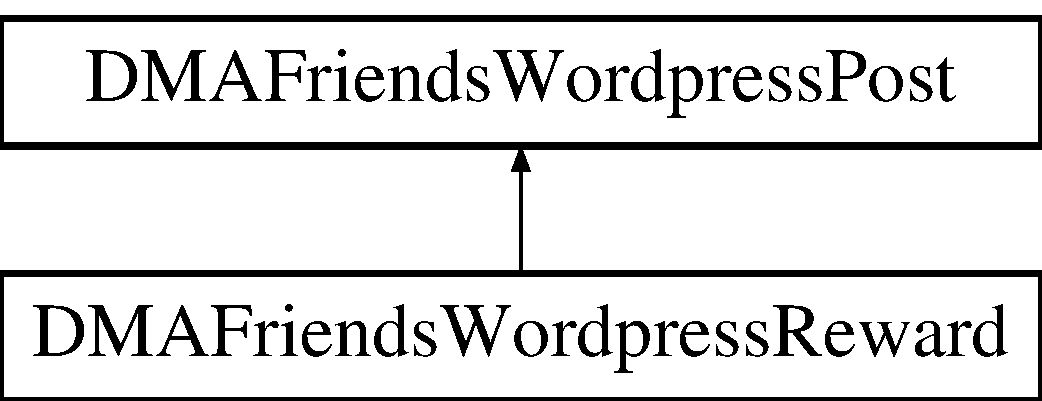
\includegraphics[height=2.000000cm]{d6/d94/classDMA_1_1Friends_1_1Wordpress_1_1Reward}
\end{center}
\end{figure}
\subsection*{Public Attributes}
\begin{DoxyCompactItemize}
\item 
\hyperlink{classDMA_1_1Friends_1_1Wordpress_1_1Reward_a653920c3f524beabf1ab4350ae09df69}{\$post\-Type} = 'badgeos-\/rewards'
\end{DoxyCompactItemize}
\subsection*{Additional Inherited Members}


\subsection{Member Data Documentation}
\hypertarget{classDMA_1_1Friends_1_1Wordpress_1_1Reward_a653920c3f524beabf1ab4350ae09df69}{\index{D\-M\-A\-::\-Friends\-::\-Wordpress\-::\-Reward@{D\-M\-A\-::\-Friends\-::\-Wordpress\-::\-Reward}!\$post\-Type@{\$post\-Type}}
\index{\$post\-Type@{\$post\-Type}!DMA::Friends::Wordpress::Reward@{D\-M\-A\-::\-Friends\-::\-Wordpress\-::\-Reward}}
\subsubsection[{\$post\-Type}]{\setlength{\rightskip}{0pt plus 5cm}D\-M\-A\textbackslash{}\-Friends\textbackslash{}\-Wordpress\textbackslash{}\-Reward\-::\$post\-Type = 'badgeos-\/rewards'}}\label{classDMA_1_1Friends_1_1Wordpress_1_1Reward_a653920c3f524beabf1ab4350ae09df69}
Override the default post type 

The documentation for this class was generated from the following file\-:\begin{DoxyCompactItemize}
\item 
wordpress/Reward.\-php\end{DoxyCompactItemize}

\hypertarget{classDMA_1_1Friends_1_1Models_1_1Reward}{\section{D\+M\+A\textbackslash{}Friends\textbackslash{}Models\textbackslash{}Reward Class Reference}
\label{classDMA_1_1Friends_1_1Models_1_1Reward}\index{D\+M\+A\textbackslash{}\+Friends\textbackslash{}\+Models\textbackslash{}\+Reward@{D\+M\+A\textbackslash{}\+Friends\textbackslash{}\+Models\textbackslash{}\+Reward}}
}
Inheritance diagram for D\+M\+A\textbackslash{}Friends\textbackslash{}Models\textbackslash{}Reward\+:\begin{figure}[H]
\begin{center}
\leavevmode
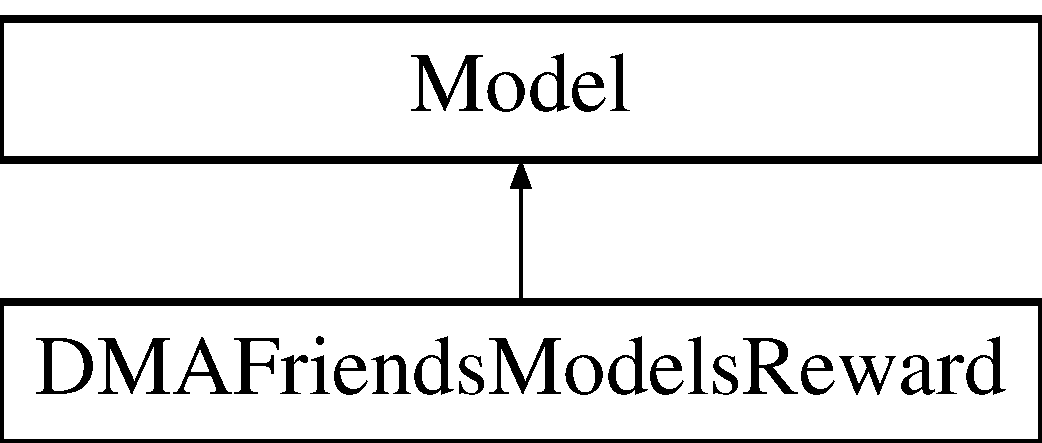
\includegraphics[height=2.000000cm]{d7/dc4/classDMA_1_1Friends_1_1Models_1_1Reward}
\end{center}
\end{figure}
\subsection*{Public Member Functions}
\begin{DoxyCompactItemize}
\item 
\hypertarget{classDMA_1_1Friends_1_1Models_1_1Reward_a672b475953c8ef5691e9c5a209204cfe}{{\bfseries scopefind\+Wordpress} (\$query, \$id)}\label{classDMA_1_1Friends_1_1Models_1_1Reward_a672b475953c8ef5691e9c5a209204cfe}

\item 
\hypertarget{classDMA_1_1Friends_1_1Models_1_1Reward_a9105978ce5ddcdc266d5023c047a72ce}{{\bfseries scope\+Is\+Active} (\$query)}\label{classDMA_1_1Friends_1_1Models_1_1Reward_a9105978ce5ddcdc266d5023c047a72ce}

\item 
\hypertarget{classDMA_1_1Friends_1_1Models_1_1Reward_a0102d2ae393a3a8c583bba79d4815103}{{\bfseries get\+Points\+Formatted\+Attribute} ()}\label{classDMA_1_1Friends_1_1Models_1_1Reward_a0102d2ae393a3a8c583bba79d4815103}

\item 
\hyperlink{classDMA_1_1Friends_1_1Models_1_1Reward_a7784ca55fbe6dd3f8b3e82da7c2e7f8f}{get\+Time\+Ago\+Attribute} (\$value)
\item 
\hypertarget{classDMA_1_1Friends_1_1Models_1_1Reward_a908a2a303004d0e42b3c2188e4999437}{{\bfseries get\+Is\+Bookmarked\+Attribute} ()}\label{classDMA_1_1Friends_1_1Models_1_1Reward_a908a2a303004d0e42b3c2188e4999437}

\item 
\hypertarget{classDMA_1_1Friends_1_1Models_1_1Reward_a463eddb6a16d6ce9e72d67441b599116}{{\bfseries get\+Email\+Template\+Options} ()}\label{classDMA_1_1Friends_1_1Models_1_1Reward_a463eddb6a16d6ce9e72d67441b599116}

\item 
\hypertarget{classDMA_1_1Friends_1_1Models_1_1Reward_afb3964195d1274580a2ae4da6461fb2c}{{\bfseries get\+Admin\+Email\+Template\+Options} ()}\label{classDMA_1_1Friends_1_1Models_1_1Reward_afb3964195d1274580a2ae4da6461fb2c}

\item 
\hypertarget{classDMA_1_1Friends_1_1Models_1_1Reward_ab68a75d9bfa49a2014632407d83d7cf0}{{\bfseries get\+Admin\+Email\+Group\+Options} ()}\label{classDMA_1_1Friends_1_1Models_1_1Reward_ab68a75d9bfa49a2014632407d83d7cf0}

\end{DoxyCompactItemize}
\subsection*{Public Attributes}
\begin{DoxyCompactItemize}
\item 
\hypertarget{classDMA_1_1Friends_1_1Models_1_1Reward_a99affaf28976dda4adc97dfe06a6c000}{{\bfseries \$table} = 'dma\+\_\+friends\+\_\+rewards'}\label{classDMA_1_1Friends_1_1Models_1_1Reward_a99affaf28976dda4adc97dfe06a6c000}

\item 
{\bfseries \$rules}
\item 
{\bfseries \$belongs\+To\+Many}
\item 
{\bfseries \$attach\+One}
\item 
{\bfseries \$morph\+Many}
\end{DoxyCompactItemize}
\subsection*{Protected Attributes}
\begin{DoxyCompactItemize}
\item 
\hypertarget{classDMA_1_1Friends_1_1Models_1_1Reward_ad1df3ebe52db8869899e29a8de5cd70d}{{\bfseries \$guarded} = \mbox{[}'$\ast$'\mbox{]}}\label{classDMA_1_1Friends_1_1Models_1_1Reward_ad1df3ebe52db8869899e29a8de5cd70d}

\item 
\hypertarget{classDMA_1_1Friends_1_1Models_1_1Reward_ae268c0f08d1cccacf8655b5028739c87}{{\bfseries \$fillable} = \mbox{[}'touch'\mbox{]}}\label{classDMA_1_1Friends_1_1Models_1_1Reward_ae268c0f08d1cccacf8655b5028739c87}

\item 
\hypertarget{classDMA_1_1Friends_1_1Models_1_1Reward_acbc452b5aadbb75acadf961a85bbc448}{{\bfseries \$dates} = \mbox{[}'date\+\_\+begin', 'date\+\_\+end'\mbox{]}}\label{classDMA_1_1Friends_1_1Models_1_1Reward_acbc452b5aadbb75acadf961a85bbc448}

\end{DoxyCompactItemize}


\subsection{Detailed Description}
\hyperlink{classDMA_1_1Friends_1_1Models_1_1Reward}{Reward} Model 

\subsection{Member Function Documentation}
\hypertarget{classDMA_1_1Friends_1_1Models_1_1Reward_a7784ca55fbe6dd3f8b3e82da7c2e7f8f}{\index{D\+M\+A\+::\+Friends\+::\+Models\+::\+Reward@{D\+M\+A\+::\+Friends\+::\+Models\+::\+Reward}!get\+Time\+Ago\+Attribute@{get\+Time\+Ago\+Attribute}}
\index{get\+Time\+Ago\+Attribute@{get\+Time\+Ago\+Attribute}!D\+M\+A\+::\+Friends\+::\+Models\+::\+Reward@{D\+M\+A\+::\+Friends\+::\+Models\+::\+Reward}}
\subsubsection[{get\+Time\+Ago\+Attribute}]{\setlength{\rightskip}{0pt plus 5cm}D\+M\+A\textbackslash{}\+Friends\textbackslash{}\+Models\textbackslash{}\+Reward\+::get\+Time\+Ago\+Attribute (
\begin{DoxyParamCaption}
\item[{}]{\$value}
\end{DoxyParamCaption}
)}}\label{classDMA_1_1Friends_1_1Models_1_1Reward_a7784ca55fbe6dd3f8b3e82da7c2e7f8f}
Mutator function to return the pivot timestamp as time ago \begin{DoxyReturn}{Returns}
string The time since the badge was earned 
\end{DoxyReturn}

\begin{DoxyCode}
77     \{
78         \textcolor{keywordflow}{if} (!isset($this->pivot->created\_at)) \textcolor{keywordflow}{return} null;
79 
80         $timeAgo = \textcolor{keyword}{new} TimeAgo;
81         \textcolor{keywordflow}{return} $timeAgo->get($this->pivot->created\_at);
82     \}
\end{DoxyCode}


\subsection{Member Data Documentation}
\hypertarget{classDMA_1_1Friends_1_1Models_1_1Reward_ab1843b31c74161b3adcb02c7be7e9556}{\index{D\+M\+A\+::\+Friends\+::\+Models\+::\+Reward@{D\+M\+A\+::\+Friends\+::\+Models\+::\+Reward}!\$attach\+One@{\$attach\+One}}
\index{\$attach\+One@{\$attach\+One}!D\+M\+A\+::\+Friends\+::\+Models\+::\+Reward@{D\+M\+A\+::\+Friends\+::\+Models\+::\+Reward}}
\subsubsection[{\$attach\+One}]{\setlength{\rightskip}{0pt plus 5cm}D\+M\+A\textbackslash{}\+Friends\textbackslash{}\+Models\textbackslash{}\+Reward\+::\$attach\+One}}\label{classDMA_1_1Friends_1_1Models_1_1Reward_ab1843b31c74161b3adcb02c7be7e9556}
{\bfseries Initial value\+:}
\begin{DoxyCode}
= [
        \textcolor{stringliteral}{'image'} => [\textcolor{stringliteral}{'System\(\backslash\)Models\(\backslash\)File'}]
    ]
\end{DoxyCode}
\hypertarget{classDMA_1_1Friends_1_1Models_1_1Reward_a4562d55136961af6257eac8242bc77a1}{\index{D\+M\+A\+::\+Friends\+::\+Models\+::\+Reward@{D\+M\+A\+::\+Friends\+::\+Models\+::\+Reward}!\$belongs\+To\+Many@{\$belongs\+To\+Many}}
\index{\$belongs\+To\+Many@{\$belongs\+To\+Many}!D\+M\+A\+::\+Friends\+::\+Models\+::\+Reward@{D\+M\+A\+::\+Friends\+::\+Models\+::\+Reward}}
\subsubsection[{\$belongs\+To\+Many}]{\setlength{\rightskip}{0pt plus 5cm}D\+M\+A\textbackslash{}\+Friends\textbackslash{}\+Models\textbackslash{}\+Reward\+::\$belongs\+To\+Many}}\label{classDMA_1_1Friends_1_1Models_1_1Reward_a4562d55136961af6257eac8242bc77a1}
{\bfseries Initial value\+:}
\begin{DoxyCode}
= [
        \textcolor{stringliteral}{'users'} => [\textcolor{stringliteral}{'Rainlab\(\backslash\)User\(\backslash\)Models\(\backslash\)User'}, \textcolor{stringliteral}{'dma\_friends\_reward\_user'}]
\end{DoxyCode}
\hypertarget{classDMA_1_1Friends_1_1Models_1_1Reward_a471e1042553519781408b0ebe6133397}{\index{D\+M\+A\+::\+Friends\+::\+Models\+::\+Reward@{D\+M\+A\+::\+Friends\+::\+Models\+::\+Reward}!\$morph\+Many@{\$morph\+Many}}
\index{\$morph\+Many@{\$morph\+Many}!D\+M\+A\+::\+Friends\+::\+Models\+::\+Reward@{D\+M\+A\+::\+Friends\+::\+Models\+::\+Reward}}
\subsubsection[{\$morph\+Many}]{\setlength{\rightskip}{0pt plus 5cm}D\+M\+A\textbackslash{}\+Friends\textbackslash{}\+Models\textbackslash{}\+Reward\+::\$morph\+Many}}\label{classDMA_1_1Friends_1_1Models_1_1Reward_a471e1042553519781408b0ebe6133397}
{\bfseries Initial value\+:}
\begin{DoxyCode}
= [ 
        \textcolor{stringliteral}{'activityLogs'}  => [\textcolor{stringliteral}{'DMA\(\backslash\)Friends\(\backslash\)Models\(\backslash\)ActivityLog'}, \textcolor{stringliteral}{'name'} => \textcolor{stringliteral}{'object'}],
        \textcolor{stringliteral}{'bookmarks'}     => [\textcolor{stringliteral}{'DMA\(\backslash\)Friends\(\backslash\)Models\(\backslash\)Bookmark'}, \textcolor{stringliteral}{'name'} => \textcolor{stringliteral}{'object'}],
    ]
\end{DoxyCode}
\hypertarget{classDMA_1_1Friends_1_1Models_1_1Reward_ab0f53a612317c68e59e32e0c4a4a2590}{\index{D\+M\+A\+::\+Friends\+::\+Models\+::\+Reward@{D\+M\+A\+::\+Friends\+::\+Models\+::\+Reward}!\$rules@{\$rules}}
\index{\$rules@{\$rules}!D\+M\+A\+::\+Friends\+::\+Models\+::\+Reward@{D\+M\+A\+::\+Friends\+::\+Models\+::\+Reward}}
\subsubsection[{\$rules}]{\setlength{\rightskip}{0pt plus 5cm}D\+M\+A\textbackslash{}\+Friends\textbackslash{}\+Models\textbackslash{}\+Reward\+::\$rules}}\label{classDMA_1_1Friends_1_1Models_1_1Reward_ab0f53a612317c68e59e32e0c4a4a2590}
{\bfseries Initial value\+:}
\begin{DoxyCode}
= [ 
        \textcolor{stringliteral}{'title'} => \textcolor{stringliteral}{'required'}
\end{DoxyCode}


The documentation for this class was generated from the following file\+:\begin{DoxyCompactItemize}
\item 
models/Reward.\+php\end{DoxyCompactItemize}

\hypertarget{classDMA_1_1Friends_1_1Api_1_1RewardResource}{\section{D\-M\-A\textbackslash{}Friends\textbackslash{}Api\textbackslash{}Reward\-Resource Class Reference}
\label{classDMA_1_1Friends_1_1Api_1_1RewardResource}\index{D\-M\-A\textbackslash{}\-Friends\textbackslash{}\-Api\textbackslash{}\-Reward\-Resource@{D\-M\-A\textbackslash{}\-Friends\textbackslash{}\-Api\textbackslash{}\-Reward\-Resource}}
}
Inheritance diagram for D\-M\-A\textbackslash{}Friends\textbackslash{}Api\textbackslash{}Reward\-Resource\-:\begin{figure}[H]
\begin{center}
\leavevmode
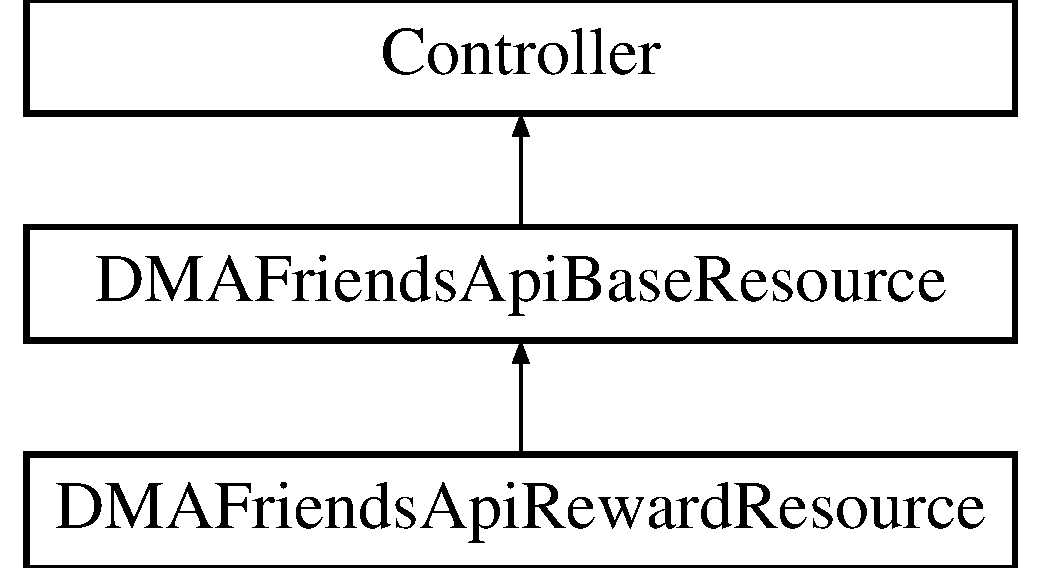
\includegraphics[height=3.000000cm]{d2/d30/classDMA_1_1Friends_1_1Api_1_1RewardResource}
\end{center}
\end{figure}
\subsection*{Protected Attributes}
\begin{DoxyCompactItemize}
\item 
\hypertarget{classDMA_1_1Friends_1_1Api_1_1RewardResource_a60661c07e9263496284122d8cd568f91}{{\bfseries \$model} = '\textbackslash{}\hyperlink{classDMA_1_1Friends_1_1Models_1_1Reward}{D\-M\-A\textbackslash{}\-Friends\textbackslash{}\-Models\textbackslash{}\-Reward}'}\label{classDMA_1_1Friends_1_1Api_1_1RewardResource_a60661c07e9263496284122d8cd568f91}

\end{DoxyCompactItemize}
\subsection*{Additional Inherited Members}


The documentation for this class was generated from the following file\-:\begin{DoxyCompactItemize}
\item 
api/Reward\-Resource.\-php\end{DoxyCompactItemize}

\hypertarget{classDMA_1_1Friends_1_1Controllers_1_1Rewards}{}\section{D\+M\+A\textbackslash{}Friends\textbackslash{}Controllers\textbackslash{}Rewards Class Reference}
\label{classDMA_1_1Friends_1_1Controllers_1_1Rewards}\index{D\+M\+A\textbackslash{}\+Friends\textbackslash{}\+Controllers\textbackslash{}\+Rewards@{D\+M\+A\textbackslash{}\+Friends\textbackslash{}\+Controllers\textbackslash{}\+Rewards}}
Inheritance diagram for D\+M\+A\textbackslash{}Friends\textbackslash{}Controllers\textbackslash{}Rewards\+:\begin{figure}[H]
\begin{center}
\leavevmode
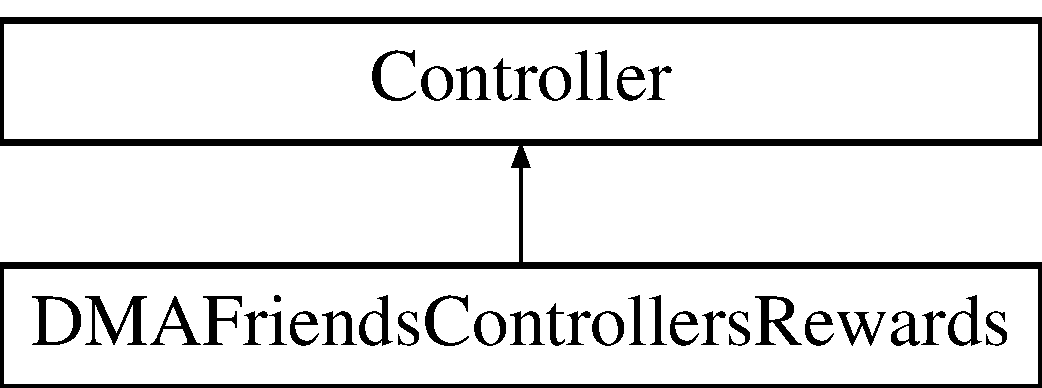
\includegraphics[height=2.000000cm]{d2/dab/classDMA_1_1Friends_1_1Controllers_1_1Rewards}
\end{center}
\end{figure}
\subsection*{Public Attributes}
\begin{DoxyCompactItemize}
\item 
{\bfseries \$implement}
\item 
\hypertarget{classDMA_1_1Friends_1_1Controllers_1_1Rewards_a9522421e338fbc2e218588583b5fb9a7}{}{\bfseries \$form\+Config} = \textquotesingle{}config\+\_\+form.\+yaml\textquotesingle{}\label{classDMA_1_1Friends_1_1Controllers_1_1Rewards_a9522421e338fbc2e218588583b5fb9a7}

\item 
\hypertarget{classDMA_1_1Friends_1_1Controllers_1_1Rewards_a887be4eff98a60ac76c7c06e4513430a}{}{\bfseries \$list\+Config} = \textquotesingle{}config\+\_\+list.\+yaml\textquotesingle{}\label{classDMA_1_1Friends_1_1Controllers_1_1Rewards_a887be4eff98a60ac76c7c06e4513430a}

\end{DoxyCompactItemize}


\subsection{Detailed Description}
\hyperlink{classDMA_1_1Friends_1_1Controllers_1_1Rewards}{Rewards} Back-\/end Controller 

\subsection{Member Data Documentation}
\hypertarget{classDMA_1_1Friends_1_1Controllers_1_1Rewards_aa3e4a1e2b9ecd667cc34ffa6de521c47}{}\index{D\+M\+A\+::\+Friends\+::\+Controllers\+::\+Rewards@{D\+M\+A\+::\+Friends\+::\+Controllers\+::\+Rewards}!\$implement@{\$implement}}
\index{\$implement@{\$implement}!D\+M\+A\+::\+Friends\+::\+Controllers\+::\+Rewards@{D\+M\+A\+::\+Friends\+::\+Controllers\+::\+Rewards}}
\subsubsection[{\$implement}]{\setlength{\rightskip}{0pt plus 5cm}D\+M\+A\textbackslash{}\+Friends\textbackslash{}\+Controllers\textbackslash{}\+Rewards\+::\$implement}\label{classDMA_1_1Friends_1_1Controllers_1_1Rewards_aa3e4a1e2b9ecd667cc34ffa6de521c47}
{\bfseries Initial value\+:}
\begin{DoxyCode}
= [
        \textcolor{stringliteral}{'Backend.Behaviors.FormController'},
        \textcolor{stringliteral}{'Backend.Behaviors.ListController'}
    ]
\end{DoxyCode}


The documentation for this class was generated from the following file\+:\begin{DoxyCompactItemize}
\item 
controllers/Rewards.\+php\end{DoxyCompactItemize}

\hypertarget{classDMA_1_1Friends_1_1Api_1_1RewardTransformer}{\section{D\-M\-A\textbackslash{}Friends\textbackslash{}Api\textbackslash{}Reward\-Transformer Class Reference}
\label{classDMA_1_1Friends_1_1Api_1_1RewardTransformer}\index{D\-M\-A\textbackslash{}\-Friends\textbackslash{}\-Api\textbackslash{}\-Reward\-Transformer@{D\-M\-A\textbackslash{}\-Friends\textbackslash{}\-Api\textbackslash{}\-Reward\-Transformer}}
}
Inheritance diagram for D\-M\-A\textbackslash{}Friends\textbackslash{}Api\textbackslash{}Reward\-Transformer\-:\begin{figure}[H]
\begin{center}
\leavevmode
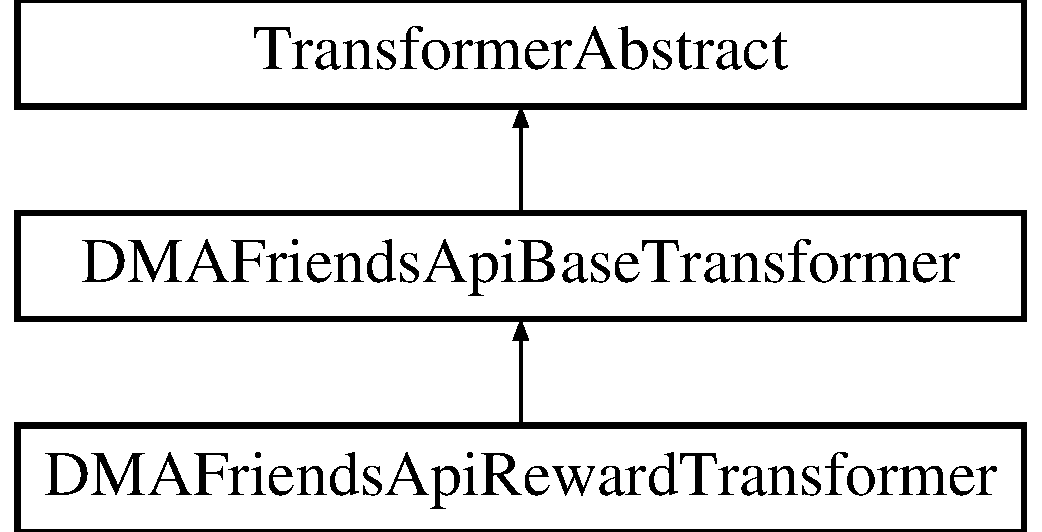
\includegraphics[height=3.000000cm]{da/d2c/classDMA_1_1Friends_1_1Api_1_1RewardTransformer}
\end{center}
\end{figure}
\subsection*{Additional Inherited Members}


The documentation for this class was generated from the following file\-:\begin{DoxyCompactItemize}
\item 
api/Reward\-Resource.\-php\end{DoxyCompactItemize}

\hypertarget{classDMA_1_1Friends_1_1Wordpress_1_1Step}{\section{D\+M\+A\textbackslash{}Friends\textbackslash{}Wordpress\textbackslash{}Step Class Reference}
\label{classDMA_1_1Friends_1_1Wordpress_1_1Step}\index{D\+M\+A\textbackslash{}\+Friends\textbackslash{}\+Wordpress\textbackslash{}\+Step@{D\+M\+A\textbackslash{}\+Friends\textbackslash{}\+Wordpress\textbackslash{}\+Step}}
}
Inheritance diagram for D\+M\+A\textbackslash{}Friends\textbackslash{}Wordpress\textbackslash{}Step\+:\begin{figure}[H]
\begin{center}
\leavevmode
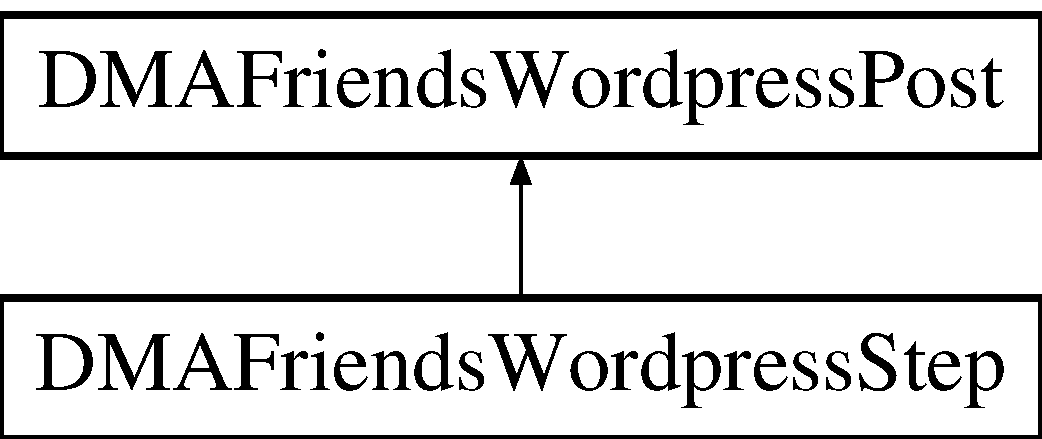
\includegraphics[height=2.000000cm]{d0/d87/classDMA_1_1Friends_1_1Wordpress_1_1Step}
\end{center}
\end{figure}
\subsection*{Public Attributes}
\begin{DoxyCompactItemize}
\item 
\hyperlink{classDMA_1_1Friends_1_1Wordpress_1_1Step_abaa142e178d837a810e5048af7f36497}{\$post\+Type} = 'step'
\end{DoxyCompactItemize}
\subsection*{Protected Attributes}
\begin{DoxyCompactItemize}
\item 
\hyperlink{classDMA_1_1Friends_1_1Wordpress_1_1Step_aa320e2b0f3f4a24c3cea41e133fd1145}{\$exclude\+Fields}
\end{DoxyCompactItemize}
\subsection*{Additional Inherited Members}


\subsection{Member Data Documentation}
\hypertarget{classDMA_1_1Friends_1_1Wordpress_1_1Step_aa320e2b0f3f4a24c3cea41e133fd1145}{\index{D\+M\+A\+::\+Friends\+::\+Wordpress\+::\+Step@{D\+M\+A\+::\+Friends\+::\+Wordpress\+::\+Step}!\$exclude\+Fields@{\$exclude\+Fields}}
\index{\$exclude\+Fields@{\$exclude\+Fields}!D\+M\+A\+::\+Friends\+::\+Wordpress\+::\+Step@{D\+M\+A\+::\+Friends\+::\+Wordpress\+::\+Step}}
\subsubsection[{\$exclude\+Fields}]{\setlength{\rightskip}{0pt plus 5cm}D\+M\+A\textbackslash{}\+Friends\textbackslash{}\+Wordpress\textbackslash{}\+Step\+::\$exclude\+Fields\hspace{0.3cm}{\ttfamily [protected]}}}\label{classDMA_1_1Friends_1_1Wordpress_1_1Step_aa320e2b0f3f4a24c3cea41e133fd1145}
{\bfseries Initial value\+:}
\begin{DoxyCode}
= [ 
        \textcolor{stringliteral}{'post\_excerpt'},
        \textcolor{stringliteral}{'post\_content'},
        \textcolor{stringliteral}{'is\_published'},
        \textcolor{stringliteral}{'post\_status'},
    ]
\end{DoxyCode}
Exclude fields from import \hypertarget{classDMA_1_1Friends_1_1Wordpress_1_1Step_abaa142e178d837a810e5048af7f36497}{\index{D\+M\+A\+::\+Friends\+::\+Wordpress\+::\+Step@{D\+M\+A\+::\+Friends\+::\+Wordpress\+::\+Step}!\$post\+Type@{\$post\+Type}}
\index{\$post\+Type@{\$post\+Type}!D\+M\+A\+::\+Friends\+::\+Wordpress\+::\+Step@{D\+M\+A\+::\+Friends\+::\+Wordpress\+::\+Step}}
\subsubsection[{\$post\+Type}]{\setlength{\rightskip}{0pt plus 5cm}D\+M\+A\textbackslash{}\+Friends\textbackslash{}\+Wordpress\textbackslash{}\+Step\+::\$post\+Type = 'step'}}\label{classDMA_1_1Friends_1_1Wordpress_1_1Step_abaa142e178d837a810e5048af7f36497}
Override the default post type 

The documentation for this class was generated from the following file\+:\begin{DoxyCompactItemize}
\item 
wordpress/Step.\+php\end{DoxyCompactItemize}

\hypertarget{classDMA_1_1Friends_1_1Models_1_1Step}{\section{D\+M\+A\textbackslash{}Friends\textbackslash{}Models\textbackslash{}Step Class Reference}
\label{classDMA_1_1Friends_1_1Models_1_1Step}\index{D\+M\+A\textbackslash{}\+Friends\textbackslash{}\+Models\textbackslash{}\+Step@{D\+M\+A\textbackslash{}\+Friends\textbackslash{}\+Models\textbackslash{}\+Step}}
}
Inheritance diagram for D\+M\+A\textbackslash{}Friends\textbackslash{}Models\textbackslash{}Step\+:\begin{figure}[H]
\begin{center}
\leavevmode
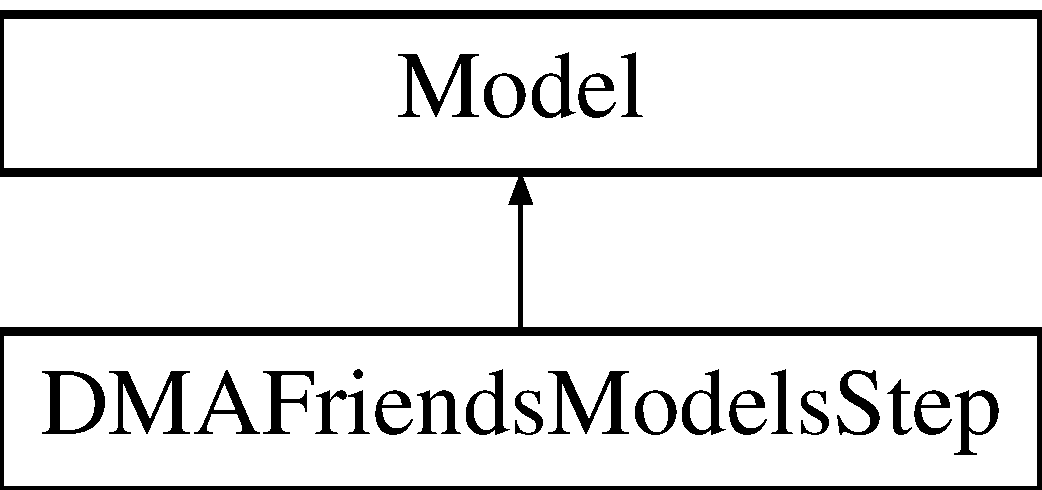
\includegraphics[height=2.000000cm]{d9/d03/classDMA_1_1Friends_1_1Models_1_1Step}
\end{center}
\end{figure}
\subsection*{Public Member Functions}
\begin{DoxyCompactItemize}
\item 
\hypertarget{classDMA_1_1Friends_1_1Models_1_1Step_a58a71b1c9b39249ac24484bbd2307db2}{{\bfseries scopefind\+Wordpress} (\$query, \$id)}\label{classDMA_1_1Friends_1_1Models_1_1Step_a58a71b1c9b39249ac24484bbd2307db2}

\end{DoxyCompactItemize}
\subsection*{Public Attributes}
\begin{DoxyCompactItemize}
\item 
\hypertarget{classDMA_1_1Friends_1_1Models_1_1Step_a73a0d48cb46b1aeeaad83499e8449acc}{{\bfseries \$table} = 'dma\+\_\+friends\+\_\+steps'}\label{classDMA_1_1Friends_1_1Models_1_1Step_a73a0d48cb46b1aeeaad83499e8449acc}

\item 
\hypertarget{classDMA_1_1Friends_1_1Models_1_1Step_a13476d5ca718080b85c9633270bf4942}{{\bfseries \$rules} = \mbox{[}$\,$\mbox{]}}\label{classDMA_1_1Friends_1_1Models_1_1Step_a13476d5ca718080b85c9633270bf4942}

\item 
{\bfseries \$belongs\+To}
\item 
{\bfseries \$belongs\+To\+Many}
\item 
{\bfseries \$morph\+Many}
\end{DoxyCompactItemize}
\subsection*{Protected Attributes}
\begin{DoxyCompactItemize}
\item 
\hypertarget{classDMA_1_1Friends_1_1Models_1_1Step_af8869edae9bea05ac3bc966d9b7debfe}{{\bfseries \$guarded} = \mbox{[}'$\ast$'\mbox{]}}\label{classDMA_1_1Friends_1_1Models_1_1Step_af8869edae9bea05ac3bc966d9b7debfe}

\item 
\hypertarget{classDMA_1_1Friends_1_1Models_1_1Step_a21b083b38af6692f21ae0827eea458a0}{{\bfseries \$fillable} = \mbox{[}'touch'\mbox{]}}\label{classDMA_1_1Friends_1_1Models_1_1Step_a21b083b38af6692f21ae0827eea458a0}

\end{DoxyCompactItemize}


\subsection{Detailed Description}
step Model 

\subsection{Member Data Documentation}
\hypertarget{classDMA_1_1Friends_1_1Models_1_1Step_a1e83eefa3362e3a1ec89b5599823c22d}{\index{D\+M\+A\+::\+Friends\+::\+Models\+::\+Step@{D\+M\+A\+::\+Friends\+::\+Models\+::\+Step}!\$belongs\+To@{\$belongs\+To}}
\index{\$belongs\+To@{\$belongs\+To}!D\+M\+A\+::\+Friends\+::\+Models\+::\+Step@{D\+M\+A\+::\+Friends\+::\+Models\+::\+Step}}
\subsubsection[{\$belongs\+To}]{\setlength{\rightskip}{0pt plus 5cm}D\+M\+A\textbackslash{}\+Friends\textbackslash{}\+Models\textbackslash{}\+Step\+::\$belongs\+To}}\label{classDMA_1_1Friends_1_1Models_1_1Step_a1e83eefa3362e3a1ec89b5599823c22d}
{\bfseries Initial value\+:}
\begin{DoxyCode}
= [
        \textcolor{stringliteral}{'activity'}  => [\textcolor{stringliteral}{'DMA\(\backslash\)Friends\(\backslash\)Models\(\backslash\)Activity'}]
\end{DoxyCode}
\hypertarget{classDMA_1_1Friends_1_1Models_1_1Step_ac0b25912a2d3c62aa72e15e443648d81}{\index{D\+M\+A\+::\+Friends\+::\+Models\+::\+Step@{D\+M\+A\+::\+Friends\+::\+Models\+::\+Step}!\$belongs\+To\+Many@{\$belongs\+To\+Many}}
\index{\$belongs\+To\+Many@{\$belongs\+To\+Many}!D\+M\+A\+::\+Friends\+::\+Models\+::\+Step@{D\+M\+A\+::\+Friends\+::\+Models\+::\+Step}}
\subsubsection[{\$belongs\+To\+Many}]{\setlength{\rightskip}{0pt plus 5cm}D\+M\+A\textbackslash{}\+Friends\textbackslash{}\+Models\textbackslash{}\+Step\+::\$belongs\+To\+Many}}\label{classDMA_1_1Friends_1_1Models_1_1Step_ac0b25912a2d3c62aa72e15e443648d81}
{\bfseries Initial value\+:}
\begin{DoxyCode}
= [
        \textcolor{stringliteral}{'users'} => [\textcolor{stringliteral}{'Rainlab\(\backslash\)User\(\backslash\)Models\(\backslash\)User'}, \textcolor{stringliteral}{'table'} => \textcolor{stringliteral}{'dma\_friends\_step\_user'}],
    ]
\end{DoxyCode}
\hypertarget{classDMA_1_1Friends_1_1Models_1_1Step_ae1aa1ff83758491327ea35861828b233}{\index{D\+M\+A\+::\+Friends\+::\+Models\+::\+Step@{D\+M\+A\+::\+Friends\+::\+Models\+::\+Step}!\$morph\+Many@{\$morph\+Many}}
\index{\$morph\+Many@{\$morph\+Many}!D\+M\+A\+::\+Friends\+::\+Models\+::\+Step@{D\+M\+A\+::\+Friends\+::\+Models\+::\+Step}}
\subsubsection[{\$morph\+Many}]{\setlength{\rightskip}{0pt plus 5cm}D\+M\+A\textbackslash{}\+Friends\textbackslash{}\+Models\textbackslash{}\+Step\+::\$morph\+Many}}\label{classDMA_1_1Friends_1_1Models_1_1Step_ae1aa1ff83758491327ea35861828b233}
{\bfseries Initial value\+:}
\begin{DoxyCode}
= [ 
        \textcolor{stringliteral}{'activityLogs'}  => [\textcolor{stringliteral}{'DMA\(\backslash\)Friends\(\backslash\)Models\(\backslash\)ActivityLog'}, \textcolor{stringliteral}{'name'} => \textcolor{stringliteral}{'object'}],
    ]
\end{DoxyCode}


The documentation for this class was generated from the following file\+:\begin{DoxyCompactItemize}
\item 
models/Step.\+php\end{DoxyCompactItemize}

\hypertarget{classDMA_1_1Friends_1_1Api_1_1StepResource}{\section{D\-M\-A\textbackslash{}Friends\textbackslash{}Api\textbackslash{}Step\-Resource Class Reference}
\label{classDMA_1_1Friends_1_1Api_1_1StepResource}\index{D\-M\-A\textbackslash{}\-Friends\textbackslash{}\-Api\textbackslash{}\-Step\-Resource@{D\-M\-A\textbackslash{}\-Friends\textbackslash{}\-Api\textbackslash{}\-Step\-Resource}}
}
Inheritance diagram for D\-M\-A\textbackslash{}Friends\textbackslash{}Api\textbackslash{}Step\-Resource\-:\begin{figure}[H]
\begin{center}
\leavevmode
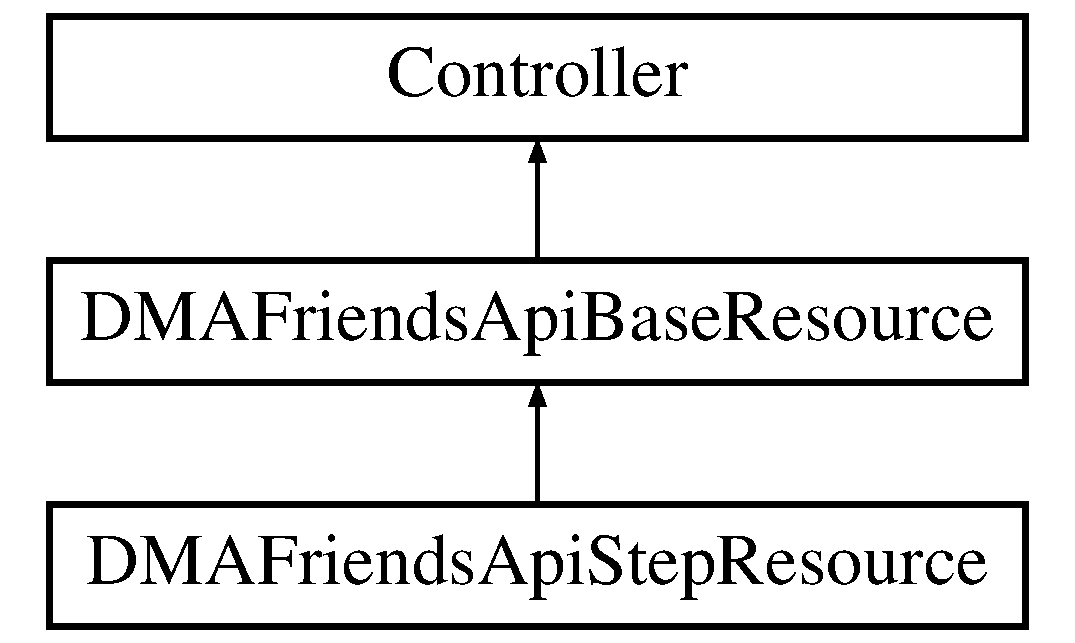
\includegraphics[height=3.000000cm]{d8/da8/classDMA_1_1Friends_1_1Api_1_1StepResource}
\end{center}
\end{figure}
\subsection*{Protected Attributes}
\begin{DoxyCompactItemize}
\item 
\hypertarget{classDMA_1_1Friends_1_1Api_1_1StepResource_a96b8c504a8e7c87634d2d33873bb9ac3}{{\bfseries \$model} = '\textbackslash{}\hyperlink{classDMA_1_1Friends_1_1Models_1_1Step}{D\-M\-A\textbackslash{}\-Friends\textbackslash{}\-Models\textbackslash{}\-Step}'}\label{classDMA_1_1Friends_1_1Api_1_1StepResource_a96b8c504a8e7c87634d2d33873bb9ac3}

\end{DoxyCompactItemize}
\subsection*{Additional Inherited Members}


The documentation for this class was generated from the following file\-:\begin{DoxyCompactItemize}
\item 
api/Step\-Resource.\-php\end{DoxyCompactItemize}

\hypertarget{classDMA_1_1Friends_1_1Controllers_1_1Steps}{\section{D\+M\+A\textbackslash{}Friends\textbackslash{}Controllers\textbackslash{}Steps Class Reference}
\label{classDMA_1_1Friends_1_1Controllers_1_1Steps}\index{D\+M\+A\textbackslash{}\+Friends\textbackslash{}\+Controllers\textbackslash{}\+Steps@{D\+M\+A\textbackslash{}\+Friends\textbackslash{}\+Controllers\textbackslash{}\+Steps}}
}
Inheritance diagram for D\+M\+A\textbackslash{}Friends\textbackslash{}Controllers\textbackslash{}Steps\+:\begin{figure}[H]
\begin{center}
\leavevmode
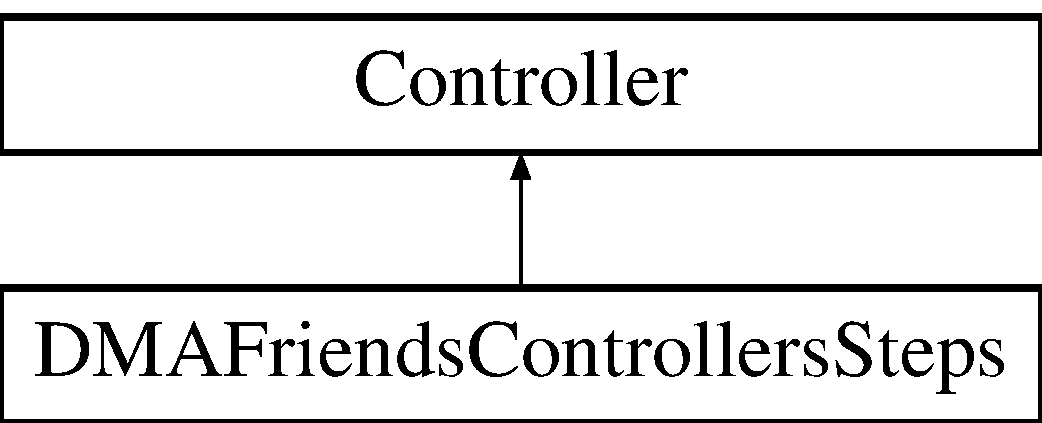
\includegraphics[height=2.000000cm]{d0/d0f/classDMA_1_1Friends_1_1Controllers_1_1Steps}
\end{center}
\end{figure}
\subsection*{Public Attributes}
\begin{DoxyCompactItemize}
\item 
{\bfseries \$implement}
\item 
\hypertarget{classDMA_1_1Friends_1_1Controllers_1_1Steps_acff6d45609493bcf45f46cbef4278190}{{\bfseries \$form\+Config} = 'config\+\_\+form.\+yaml'}\label{classDMA_1_1Friends_1_1Controllers_1_1Steps_acff6d45609493bcf45f46cbef4278190}

\item 
\hypertarget{classDMA_1_1Friends_1_1Controllers_1_1Steps_a1ff81739bf6107eccb4b3885aa6f7008}{{\bfseries \$list\+Config} = 'config\+\_\+list.\+yaml'}\label{classDMA_1_1Friends_1_1Controllers_1_1Steps_a1ff81739bf6107eccb4b3885aa6f7008}

\end{DoxyCompactItemize}


\subsection{Detailed Description}
\hyperlink{classDMA_1_1Friends_1_1Controllers_1_1Steps}{Steps} Back-\/end Controller 

\subsection{Member Data Documentation}
\hypertarget{classDMA_1_1Friends_1_1Controllers_1_1Steps_a49cada3b2a4350d576cd15aa2f5d1ce6}{\index{D\+M\+A\+::\+Friends\+::\+Controllers\+::\+Steps@{D\+M\+A\+::\+Friends\+::\+Controllers\+::\+Steps}!\$implement@{\$implement}}
\index{\$implement@{\$implement}!D\+M\+A\+::\+Friends\+::\+Controllers\+::\+Steps@{D\+M\+A\+::\+Friends\+::\+Controllers\+::\+Steps}}
\subsubsection[{\$implement}]{\setlength{\rightskip}{0pt plus 5cm}D\+M\+A\textbackslash{}\+Friends\textbackslash{}\+Controllers\textbackslash{}\+Steps\+::\$implement}}\label{classDMA_1_1Friends_1_1Controllers_1_1Steps_a49cada3b2a4350d576cd15aa2f5d1ce6}
{\bfseries Initial value\+:}
\begin{DoxyCode}
= [
        \textcolor{stringliteral}{'Backend.Behaviors.FormController'},
        \textcolor{stringliteral}{'Backend.Behaviors.ListController'}
    ]
\end{DoxyCode}


The documentation for this class was generated from the following file\+:\begin{DoxyCompactItemize}
\item 
controllers/Steps.\+php\end{DoxyCompactItemize}

\hypertarget{classDMA_1_1Friends_1_1Api_1_1StepTransformer}{\section{D\-M\-A\textbackslash{}Friends\textbackslash{}Api\textbackslash{}Step\-Transformer Class Reference}
\label{classDMA_1_1Friends_1_1Api_1_1StepTransformer}\index{D\-M\-A\textbackslash{}\-Friends\textbackslash{}\-Api\textbackslash{}\-Step\-Transformer@{D\-M\-A\textbackslash{}\-Friends\textbackslash{}\-Api\textbackslash{}\-Step\-Transformer}}
}
Inheritance diagram for D\-M\-A\textbackslash{}Friends\textbackslash{}Api\textbackslash{}Step\-Transformer\-:\begin{figure}[H]
\begin{center}
\leavevmode
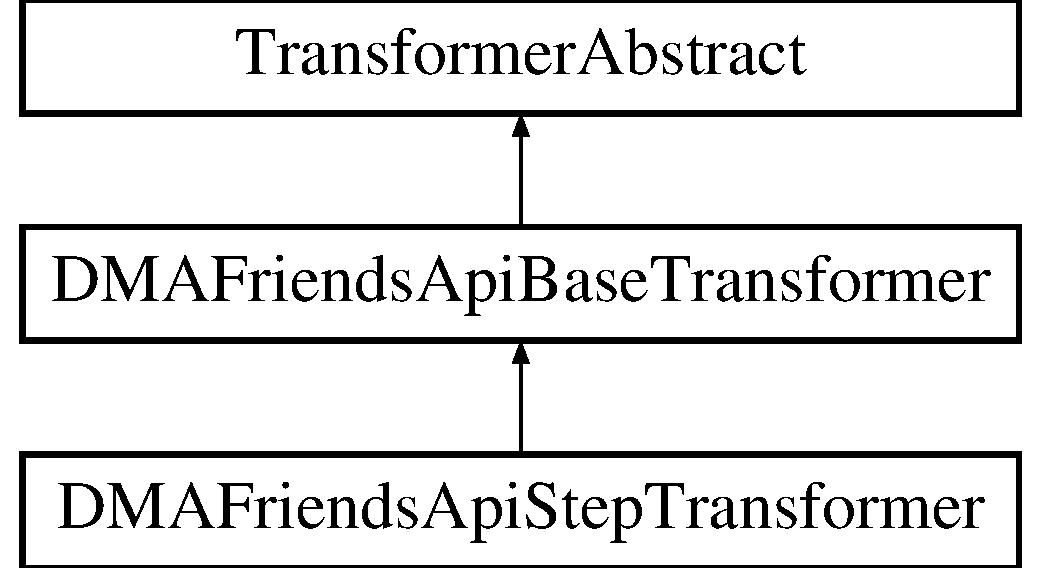
\includegraphics[height=3.000000cm]{d0/dbc/classDMA_1_1Friends_1_1Api_1_1StepTransformer}
\end{center}
\end{figure}
\subsection*{Additional Inherited Members}


The documentation for this class was generated from the following file\-:\begin{DoxyCompactItemize}
\item 
api/Step\-Resource.\-php\end{DoxyCompactItemize}

\hypertarget{classDMA_1_1Friends_1_1Console_1_1SyncFriendsDataCommand}{\section{D\-M\-A\textbackslash{}Friends\textbackslash{}Console\textbackslash{}Sync\-Friends\-Data\-Command Class Reference}
\label{classDMA_1_1Friends_1_1Console_1_1SyncFriendsDataCommand}\index{D\-M\-A\textbackslash{}\-Friends\textbackslash{}\-Console\textbackslash{}\-Sync\-Friends\-Data\-Command@{D\-M\-A\textbackslash{}\-Friends\textbackslash{}\-Console\textbackslash{}\-Sync\-Friends\-Data\-Command}}
}
Inheritance diagram for D\-M\-A\textbackslash{}Friends\textbackslash{}Console\textbackslash{}Sync\-Friends\-Data\-Command\-:\begin{figure}[H]
\begin{center}
\leavevmode
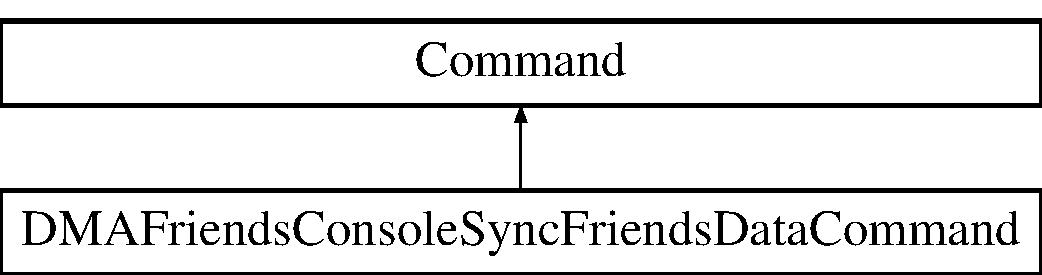
\includegraphics[height=2.000000cm]{d1/dfb/classDMA_1_1Friends_1_1Console_1_1SyncFriendsDataCommand}
\end{center}
\end{figure}
\subsection*{Public Member Functions}
\begin{DoxyCompactItemize}
\item 
\hyperlink{classDMA_1_1Friends_1_1Console_1_1SyncFriendsDataCommand_a1fba6962dc1edd7eca63cd6d467f53b9}{\-\_\-\-\_\-construct} ()
\item 
\hyperlink{classDMA_1_1Friends_1_1Console_1_1SyncFriendsDataCommand_acadcd5594f052ee5f2604834ddc8c5cb}{fire} ()
\end{DoxyCompactItemize}
\subsection*{Protected Member Functions}
\begin{DoxyCompactItemize}
\item 
\hyperlink{classDMA_1_1Friends_1_1Console_1_1SyncFriendsDataCommand_a1eae022ca4e5682380177d5d5766849c}{sync\-Users} ()
\item 
\hyperlink{classDMA_1_1Friends_1_1Console_1_1SyncFriendsDataCommand_a6096678a576ae660cf9f77939d1a7a0a}{sync\-Activities} ()
\item 
\hyperlink{classDMA_1_1Friends_1_1Console_1_1SyncFriendsDataCommand_a02c61f10c3ad4f533922d28764a87c23}{sync\-Activity\-Logs} ()
\item 
\hyperlink{classDMA_1_1Friends_1_1Console_1_1SyncFriendsDataCommand_acfe572a5dac71f39f215bf6aadae6921}{sync\-Badges} ()
\item 
\hyperlink{classDMA_1_1Friends_1_1Console_1_1SyncFriendsDataCommand_a8472e8b840eb743488e60df0789ef322}{sync\-Locations} ()
\item 
\hyperlink{classDMA_1_1Friends_1_1Console_1_1SyncFriendsDataCommand_af91f14f7db12896473d70a025aa0d8e2}{sync\-Rewards} ()
\item 
\hyperlink{classDMA_1_1Friends_1_1Console_1_1SyncFriendsDataCommand_ad4357326e1637c41b084551a7cfb90df}{sync\-Steps} ()
\item 
\hypertarget{classDMA_1_1Friends_1_1Console_1_1SyncFriendsDataCommand_afe4181b04f8fd685846c4dcbe8a8a740}{{\bfseries sync} (\$model, \$text\-Type)}\label{classDMA_1_1Friends_1_1Console_1_1SyncFriendsDataCommand_afe4181b04f8fd685846c4dcbe8a8a740}

\item 
\hyperlink{classDMA_1_1Friends_1_1Console_1_1SyncFriendsDataCommand_a3ccde1f8b688921d950c3ec45569e920}{get\-Options} ()
\end{DoxyCompactItemize}
\subsection*{Protected Attributes}
\begin{DoxyCompactItemize}
\item 
\hypertarget{classDMA_1_1Friends_1_1Console_1_1SyncFriendsDataCommand_aa809c8407f33bc5c85ad36397e58a9ac}{{\bfseries \$name} = 'friends\-:sync-\/data'}\label{classDMA_1_1Friends_1_1Console_1_1SyncFriendsDataCommand_aa809c8407f33bc5c85ad36397e58a9ac}

\item 
\hypertarget{classDMA_1_1Friends_1_1Console_1_1SyncFriendsDataCommand_af193515d33918a06da0fd5ebb4893fa9}{{\bfseries \$description} = 'Syncronize wordpress data into October'}\label{classDMA_1_1Friends_1_1Console_1_1SyncFriendsDataCommand_af193515d33918a06da0fd5ebb4893fa9}

\item 
\hypertarget{classDMA_1_1Friends_1_1Console_1_1SyncFriendsDataCommand_a024b40c42d09505fba54a8bc4c1d8384}{{\bfseries \$db} = null}\label{classDMA_1_1Friends_1_1Console_1_1SyncFriendsDataCommand_a024b40c42d09505fba54a8bc4c1d8384}

\item 
\hypertarget{classDMA_1_1Friends_1_1Console_1_1SyncFriendsDataCommand_a2403b0723b3478b2975a61020f5264cb}{{\bfseries \$limit} = 1000}\label{classDMA_1_1Friends_1_1Console_1_1SyncFriendsDataCommand_a2403b0723b3478b2975a61020f5264cb}

\end{DoxyCompactItemize}


\subsection{Constructor \& Destructor Documentation}
\hypertarget{classDMA_1_1Friends_1_1Console_1_1SyncFriendsDataCommand_a1fba6962dc1edd7eca63cd6d467f53b9}{\index{D\-M\-A\-::\-Friends\-::\-Console\-::\-Sync\-Friends\-Data\-Command@{D\-M\-A\-::\-Friends\-::\-Console\-::\-Sync\-Friends\-Data\-Command}!\-\_\-\-\_\-construct@{\-\_\-\-\_\-construct}}
\index{\-\_\-\-\_\-construct@{\-\_\-\-\_\-construct}!DMA::Friends::Console::SyncFriendsDataCommand@{D\-M\-A\-::\-Friends\-::\-Console\-::\-Sync\-Friends\-Data\-Command}}
\subsubsection[{\-\_\-\-\_\-construct}]{\setlength{\rightskip}{0pt plus 5cm}D\-M\-A\textbackslash{}\-Friends\textbackslash{}\-Console\textbackslash{}\-Sync\-Friends\-Data\-Command\-::\-\_\-\-\_\-construct (
\begin{DoxyParamCaption}
{}
\end{DoxyParamCaption}
)}}\label{classDMA_1_1Friends_1_1Console_1_1SyncFriendsDataCommand_a1fba6962dc1edd7eca63cd6d467f53b9}
Create a new command instance. \begin{DoxyReturn}{Returns}
void 
\end{DoxyReturn}

\begin{DoxyCode}
46     \{
47         $this->db = DB::connection(\textcolor{stringliteral}{'friends\_wordpress'});
48 
49         parent::\_\_construct();
50     \}
\end{DoxyCode}


\subsection{Member Function Documentation}
\hypertarget{classDMA_1_1Friends_1_1Console_1_1SyncFriendsDataCommand_acadcd5594f052ee5f2604834ddc8c5cb}{\index{D\-M\-A\-::\-Friends\-::\-Console\-::\-Sync\-Friends\-Data\-Command@{D\-M\-A\-::\-Friends\-::\-Console\-::\-Sync\-Friends\-Data\-Command}!fire@{fire}}
\index{fire@{fire}!DMA::Friends::Console::SyncFriendsDataCommand@{D\-M\-A\-::\-Friends\-::\-Console\-::\-Sync\-Friends\-Data\-Command}}
\subsubsection[{fire}]{\setlength{\rightskip}{0pt plus 5cm}D\-M\-A\textbackslash{}\-Friends\textbackslash{}\-Console\textbackslash{}\-Sync\-Friends\-Data\-Command\-::fire (
\begin{DoxyParamCaption}
{}
\end{DoxyParamCaption}
)}}\label{classDMA_1_1Friends_1_1Console_1_1SyncFriendsDataCommand_acadcd5594f052ee5f2604834ddc8c5cb}
Execute the console command. \begin{DoxyReturn}{Returns}
void 
\end{DoxyReturn}

\begin{DoxyCode}
57     \{
58 
59         $type = $this->option(\textcolor{stringliteral}{'type'});
60         $this->limit = $this->option(\textcolor{stringliteral}{'limit'});
61 
62         \textcolor{keywordflow}{switch}($type) \{
63             \textcolor{keywordflow}{case} \textcolor{stringliteral}{'users'}:
64                 $this->\hyperlink{classDMA_1_1Friends_1_1Console_1_1SyncFriendsDataCommand_a1eae022ca4e5682380177d5d5766849c}{syncUsers}();
65                 \textcolor{keywordflow}{break};
66             \textcolor{keywordflow}{case} \textcolor{stringliteral}{'activities'}:
67                 $this->\hyperlink{classDMA_1_1Friends_1_1Console_1_1SyncFriendsDataCommand_a6096678a576ae660cf9f77939d1a7a0a}{syncActivities}();
68                 \textcolor{keywordflow}{break};
69             \textcolor{keywordflow}{case} \textcolor{stringliteral}{'activity-logs'}:
70                 $this->\hyperlink{classDMA_1_1Friends_1_1Console_1_1SyncFriendsDataCommand_a02c61f10c3ad4f533922d28764a87c23}{syncActivityLogs}();
71                 \textcolor{keywordflow}{break};
72             \textcolor{keywordflow}{case} \textcolor{stringliteral}{'badges'}:
73                 $this->\hyperlink{classDMA_1_1Friends_1_1Console_1_1SyncFriendsDataCommand_acfe572a5dac71f39f215bf6aadae6921}{syncBadges}();
74                 \textcolor{keywordflow}{break};
75             \textcolor{keywordflow}{case} \textcolor{stringliteral}{'locations'}:
76                 $this->\hyperlink{classDMA_1_1Friends_1_1Console_1_1SyncFriendsDataCommand_a8472e8b840eb743488e60df0789ef322}{syncLocations}();
77                 \textcolor{keywordflow}{break};
78             \textcolor{keywordflow}{case} \textcolor{stringliteral}{'rewards'}:
79                 $this->\hyperlink{classDMA_1_1Friends_1_1Console_1_1SyncFriendsDataCommand_af91f14f7db12896473d70a025aa0d8e2}{syncRewards}();
80                 \textcolor{keywordflow}{break};
81             \textcolor{keywordflow}{case} \textcolor{stringliteral}{'steps'}:
82                 $this->\hyperlink{classDMA_1_1Friends_1_1Console_1_1SyncFriendsDataCommand_ad4357326e1637c41b084551a7cfb90df}{syncSteps}();
83                 \textcolor{keywordflow}{break};
84             \textcolor{keywordflow}{default}:
85                 $this->\hyperlink{classDMA_1_1Friends_1_1Console_1_1SyncFriendsDataCommand_a1eae022ca4e5682380177d5d5766849c}{syncUsers}();
86                 $this->\hyperlink{classDMA_1_1Friends_1_1Console_1_1SyncFriendsDataCommand_a6096678a576ae660cf9f77939d1a7a0a}{syncActivities}();
87                 $this->\hyperlink{classDMA_1_1Friends_1_1Console_1_1SyncFriendsDataCommand_a02c61f10c3ad4f533922d28764a87c23}{syncActivityLogs}();
88                 $this->\hyperlink{classDMA_1_1Friends_1_1Console_1_1SyncFriendsDataCommand_acfe572a5dac71f39f215bf6aadae6921}{syncBadges}();
89                 $this->\hyperlink{classDMA_1_1Friends_1_1Console_1_1SyncFriendsDataCommand_a8472e8b840eb743488e60df0789ef322}{syncLocations}();
90                 $this->\hyperlink{classDMA_1_1Friends_1_1Console_1_1SyncFriendsDataCommand_af91f14f7db12896473d70a025aa0d8e2}{syncRewards}();
91                 $this->\hyperlink{classDMA_1_1Friends_1_1Console_1_1SyncFriendsDataCommand_ad4357326e1637c41b084551a7cfb90df}{syncSteps}();
92         \}
93 
94         $this->output->writeln(\textcolor{stringliteral}{'Sync complete'});
95     \}
\end{DoxyCode}
\hypertarget{classDMA_1_1Friends_1_1Console_1_1SyncFriendsDataCommand_a3ccde1f8b688921d950c3ec45569e920}{\index{D\-M\-A\-::\-Friends\-::\-Console\-::\-Sync\-Friends\-Data\-Command@{D\-M\-A\-::\-Friends\-::\-Console\-::\-Sync\-Friends\-Data\-Command}!get\-Options@{get\-Options}}
\index{get\-Options@{get\-Options}!DMA::Friends::Console::SyncFriendsDataCommand@{D\-M\-A\-::\-Friends\-::\-Console\-::\-Sync\-Friends\-Data\-Command}}
\subsubsection[{get\-Options}]{\setlength{\rightskip}{0pt plus 5cm}D\-M\-A\textbackslash{}\-Friends\textbackslash{}\-Console\textbackslash{}\-Sync\-Friends\-Data\-Command\-::get\-Options (
\begin{DoxyParamCaption}
{}
\end{DoxyParamCaption}
)\hspace{0.3cm}{\ttfamily [protected]}}}\label{classDMA_1_1Friends_1_1Console_1_1SyncFriendsDataCommand_a3ccde1f8b688921d950c3ec45569e920}
Get the console command options. \begin{DoxyReturn}{Returns}
array 
\end{DoxyReturn}

\begin{DoxyCode}
179     \{   
180         \textcolor{keywordflow}{return} [
181             [\textcolor{stringliteral}{'type'}, null, InputOption::VALUE\_OPTIONAL, \textcolor{stringliteral}{'Import specific type'}, null],
182             [\textcolor{stringliteral}{'limit'}, null, InputOption::VALUE\_OPTIONAL, \textcolor{stringliteral}{'Number of records per type to import'}, 
      $this->limit],
183         ];  
184     \}  
\end{DoxyCode}
\hypertarget{classDMA_1_1Friends_1_1Console_1_1SyncFriendsDataCommand_a6096678a576ae660cf9f77939d1a7a0a}{\index{D\-M\-A\-::\-Friends\-::\-Console\-::\-Sync\-Friends\-Data\-Command@{D\-M\-A\-::\-Friends\-::\-Console\-::\-Sync\-Friends\-Data\-Command}!sync\-Activities@{sync\-Activities}}
\index{sync\-Activities@{sync\-Activities}!DMA::Friends::Console::SyncFriendsDataCommand@{D\-M\-A\-::\-Friends\-::\-Console\-::\-Sync\-Friends\-Data\-Command}}
\subsubsection[{sync\-Activities}]{\setlength{\rightskip}{0pt plus 5cm}D\-M\-A\textbackslash{}\-Friends\textbackslash{}\-Console\textbackslash{}\-Sync\-Friends\-Data\-Command\-::sync\-Activities (
\begin{DoxyParamCaption}
{}
\end{DoxyParamCaption}
)\hspace{0.3cm}{\ttfamily [protected]}}}\label{classDMA_1_1Friends_1_1Console_1_1SyncFriendsDataCommand_a6096678a576ae660cf9f77939d1a7a0a}
Syncronize wordpress activities with laravel \begin{DoxyReturn}{Returns}
int 
\end{DoxyReturn}

\begin{DoxyCode}
112     \{
113         $activities = \textcolor{keyword}{new} WordpressActivity;
114         $this->sync($activities, \textcolor{stringliteral}{'activities'});
115     \}
\end{DoxyCode}
\hypertarget{classDMA_1_1Friends_1_1Console_1_1SyncFriendsDataCommand_a02c61f10c3ad4f533922d28764a87c23}{\index{D\-M\-A\-::\-Friends\-::\-Console\-::\-Sync\-Friends\-Data\-Command@{D\-M\-A\-::\-Friends\-::\-Console\-::\-Sync\-Friends\-Data\-Command}!sync\-Activity\-Logs@{sync\-Activity\-Logs}}
\index{sync\-Activity\-Logs@{sync\-Activity\-Logs}!DMA::Friends::Console::SyncFriendsDataCommand@{D\-M\-A\-::\-Friends\-::\-Console\-::\-Sync\-Friends\-Data\-Command}}
\subsubsection[{sync\-Activity\-Logs}]{\setlength{\rightskip}{0pt plus 5cm}D\-M\-A\textbackslash{}\-Friends\textbackslash{}\-Console\textbackslash{}\-Sync\-Friends\-Data\-Command\-::sync\-Activity\-Logs (
\begin{DoxyParamCaption}
{}
\end{DoxyParamCaption}
)\hspace{0.3cm}{\ttfamily [protected]}}}\label{classDMA_1_1Friends_1_1Console_1_1SyncFriendsDataCommand_a02c61f10c3ad4f533922d28764a87c23}
Syncronize Badge\-O\-S Activity Logs with laravel \begin{DoxyReturn}{Returns}
int 
\end{DoxyReturn}

\begin{DoxyCode}
122     \{
123         $activityLogs = \textcolor{keyword}{new} WordpressActivityLog;
124         $this->sync($activityLogs, \textcolor{stringliteral}{'activity logs'});
125 
126     \}
\end{DoxyCode}
\hypertarget{classDMA_1_1Friends_1_1Console_1_1SyncFriendsDataCommand_acfe572a5dac71f39f215bf6aadae6921}{\index{D\-M\-A\-::\-Friends\-::\-Console\-::\-Sync\-Friends\-Data\-Command@{D\-M\-A\-::\-Friends\-::\-Console\-::\-Sync\-Friends\-Data\-Command}!sync\-Badges@{sync\-Badges}}
\index{sync\-Badges@{sync\-Badges}!DMA::Friends::Console::SyncFriendsDataCommand@{D\-M\-A\-::\-Friends\-::\-Console\-::\-Sync\-Friends\-Data\-Command}}
\subsubsection[{sync\-Badges}]{\setlength{\rightskip}{0pt plus 5cm}D\-M\-A\textbackslash{}\-Friends\textbackslash{}\-Console\textbackslash{}\-Sync\-Friends\-Data\-Command\-::sync\-Badges (
\begin{DoxyParamCaption}
{}
\end{DoxyParamCaption}
)\hspace{0.3cm}{\ttfamily [protected]}}}\label{classDMA_1_1Friends_1_1Console_1_1SyncFriendsDataCommand_acfe572a5dac71f39f215bf6aadae6921}
Syncronize wordpress badges with laravel \begin{DoxyReturn}{Returns}
int 
\end{DoxyReturn}

\begin{DoxyCode}
133     \{
134         $badges = \textcolor{keyword}{new} WordpressBadge;
135         $this->sync($badges, \textcolor{stringliteral}{'badges'});
136     \}
\end{DoxyCode}
\hypertarget{classDMA_1_1Friends_1_1Console_1_1SyncFriendsDataCommand_a8472e8b840eb743488e60df0789ef322}{\index{D\-M\-A\-::\-Friends\-::\-Console\-::\-Sync\-Friends\-Data\-Command@{D\-M\-A\-::\-Friends\-::\-Console\-::\-Sync\-Friends\-Data\-Command}!sync\-Locations@{sync\-Locations}}
\index{sync\-Locations@{sync\-Locations}!DMA::Friends::Console::SyncFriendsDataCommand@{D\-M\-A\-::\-Friends\-::\-Console\-::\-Sync\-Friends\-Data\-Command}}
\subsubsection[{sync\-Locations}]{\setlength{\rightskip}{0pt plus 5cm}D\-M\-A\textbackslash{}\-Friends\textbackslash{}\-Console\textbackslash{}\-Sync\-Friends\-Data\-Command\-::sync\-Locations (
\begin{DoxyParamCaption}
{}
\end{DoxyParamCaption}
)\hspace{0.3cm}{\ttfamily [protected]}}}\label{classDMA_1_1Friends_1_1Console_1_1SyncFriendsDataCommand_a8472e8b840eb743488e60df0789ef322}
Syncronize wordpress locations with laravel \begin{DoxyReturn}{Returns}
int 
\end{DoxyReturn}

\begin{DoxyCode}
143     \{   
144         $locations = \textcolor{keyword}{new} WordpressLocation;
145         $this->sync($locations, \textcolor{stringliteral}{'locations'});
146     \}  
\end{DoxyCode}
\hypertarget{classDMA_1_1Friends_1_1Console_1_1SyncFriendsDataCommand_af91f14f7db12896473d70a025aa0d8e2}{\index{D\-M\-A\-::\-Friends\-::\-Console\-::\-Sync\-Friends\-Data\-Command@{D\-M\-A\-::\-Friends\-::\-Console\-::\-Sync\-Friends\-Data\-Command}!sync\-Rewards@{sync\-Rewards}}
\index{sync\-Rewards@{sync\-Rewards}!DMA::Friends::Console::SyncFriendsDataCommand@{D\-M\-A\-::\-Friends\-::\-Console\-::\-Sync\-Friends\-Data\-Command}}
\subsubsection[{sync\-Rewards}]{\setlength{\rightskip}{0pt plus 5cm}D\-M\-A\textbackslash{}\-Friends\textbackslash{}\-Console\textbackslash{}\-Sync\-Friends\-Data\-Command\-::sync\-Rewards (
\begin{DoxyParamCaption}
{}
\end{DoxyParamCaption}
)\hspace{0.3cm}{\ttfamily [protected]}}}\label{classDMA_1_1Friends_1_1Console_1_1SyncFriendsDataCommand_af91f14f7db12896473d70a025aa0d8e2}
Syncronize wordpress rewards with laravel \begin{DoxyReturn}{Returns}
int 
\end{DoxyReturn}

\begin{DoxyCode}
153     \{   
154         $rewards = \textcolor{keyword}{new} WordpressReward;
155         $this->sync($rewards, \textcolor{stringliteral}{'rewards'});
156     \}  
\end{DoxyCode}
\hypertarget{classDMA_1_1Friends_1_1Console_1_1SyncFriendsDataCommand_ad4357326e1637c41b084551a7cfb90df}{\index{D\-M\-A\-::\-Friends\-::\-Console\-::\-Sync\-Friends\-Data\-Command@{D\-M\-A\-::\-Friends\-::\-Console\-::\-Sync\-Friends\-Data\-Command}!sync\-Steps@{sync\-Steps}}
\index{sync\-Steps@{sync\-Steps}!DMA::Friends::Console::SyncFriendsDataCommand@{D\-M\-A\-::\-Friends\-::\-Console\-::\-Sync\-Friends\-Data\-Command}}
\subsubsection[{sync\-Steps}]{\setlength{\rightskip}{0pt plus 5cm}D\-M\-A\textbackslash{}\-Friends\textbackslash{}\-Console\textbackslash{}\-Sync\-Friends\-Data\-Command\-::sync\-Steps (
\begin{DoxyParamCaption}
{}
\end{DoxyParamCaption}
)\hspace{0.3cm}{\ttfamily [protected]}}}\label{classDMA_1_1Friends_1_1Console_1_1SyncFriendsDataCommand_ad4357326e1637c41b084551a7cfb90df}
Syncronize wordpress steps with laravel \begin{DoxyReturn}{Returns}
int 
\end{DoxyReturn}

\begin{DoxyCode}
163     \{   
164         $steps = \textcolor{keyword}{new} WordpressStep;
165         $this->sync($steps, \textcolor{stringliteral}{'steps'});
166     \}  
\end{DoxyCode}
\hypertarget{classDMA_1_1Friends_1_1Console_1_1SyncFriendsDataCommand_a1eae022ca4e5682380177d5d5766849c}{\index{D\-M\-A\-::\-Friends\-::\-Console\-::\-Sync\-Friends\-Data\-Command@{D\-M\-A\-::\-Friends\-::\-Console\-::\-Sync\-Friends\-Data\-Command}!sync\-Users@{sync\-Users}}
\index{sync\-Users@{sync\-Users}!DMA::Friends::Console::SyncFriendsDataCommand@{D\-M\-A\-::\-Friends\-::\-Console\-::\-Sync\-Friends\-Data\-Command}}
\subsubsection[{sync\-Users}]{\setlength{\rightskip}{0pt plus 5cm}D\-M\-A\textbackslash{}\-Friends\textbackslash{}\-Console\textbackslash{}\-Sync\-Friends\-Data\-Command\-::sync\-Users (
\begin{DoxyParamCaption}
{}
\end{DoxyParamCaption}
)\hspace{0.3cm}{\ttfamily [protected]}}}\label{classDMA_1_1Friends_1_1Console_1_1SyncFriendsDataCommand_a1eae022ca4e5682380177d5d5766849c}
Syncronize wordpress user accounts with laravel 
\begin{DoxyCode}
101     \{
102         $user = \textcolor{keyword}{new} WordpressUser;
103         $user->updateExistingUsers();
104         $this->sync($user, \textcolor{stringliteral}{'users'});
105     \}
\end{DoxyCode}


The documentation for this class was generated from the following file\-:\begin{DoxyCompactItemize}
\item 
console/Sync\-Friends\-Data\-Command.\-php\end{DoxyCompactItemize}

\hypertarget{classDMA_1_1Friends_1_1Console_1_1SyncFriendsRelationsCommand}{\section{D\-M\-A\textbackslash{}Friends\textbackslash{}Console\textbackslash{}Sync\-Friends\-Relations\-Command Class Reference}
\label{classDMA_1_1Friends_1_1Console_1_1SyncFriendsRelationsCommand}\index{D\-M\-A\textbackslash{}\-Friends\textbackslash{}\-Console\textbackslash{}\-Sync\-Friends\-Relations\-Command@{D\-M\-A\textbackslash{}\-Friends\textbackslash{}\-Console\textbackslash{}\-Sync\-Friends\-Relations\-Command}}
}
Inheritance diagram for D\-M\-A\textbackslash{}Friends\textbackslash{}Console\textbackslash{}Sync\-Friends\-Relations\-Command\-:\begin{figure}[H]
\begin{center}
\leavevmode
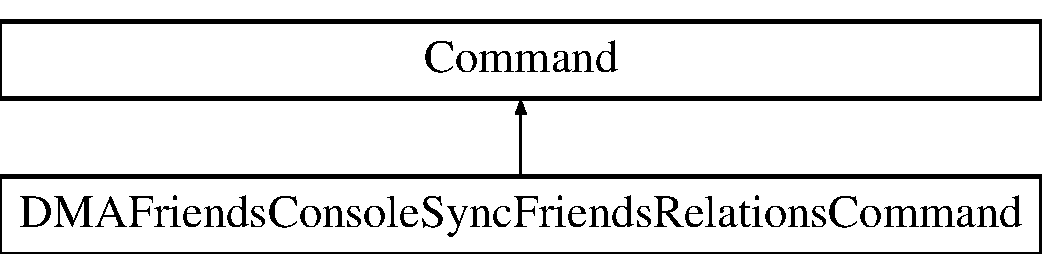
\includegraphics[height=2.000000cm]{d5/dee/classDMA_1_1Friends_1_1Console_1_1SyncFriendsRelationsCommand}
\end{center}
\end{figure}
\subsection*{Public Member Functions}
\begin{DoxyCompactItemize}
\item 
\hyperlink{classDMA_1_1Friends_1_1Console_1_1SyncFriendsRelationsCommand_ad7d4bd66608d25ccd00ce87331287183}{\-\_\-\-\_\-construct} ()
\item 
\hyperlink{classDMA_1_1Friends_1_1Console_1_1SyncFriendsRelationsCommand_a075f13536ecb959b0a54c2e74822e35c}{fire} ()
\end{DoxyCompactItemize}
\subsection*{Protected Attributes}
\begin{DoxyCompactItemize}
\item 
\hypertarget{classDMA_1_1Friends_1_1Console_1_1SyncFriendsRelationsCommand_a831e5df8629b4803f5dc6e007112f8b9}{{\bfseries \$name} = 'friends\-:sync-\/relations'}\label{classDMA_1_1Friends_1_1Console_1_1SyncFriendsRelationsCommand_a831e5df8629b4803f5dc6e007112f8b9}

\item 
\hypertarget{classDMA_1_1Friends_1_1Console_1_1SyncFriendsRelationsCommand_af90161ad028e6dd9e8d0dc51d82ef903}{{\bfseries \$description} = 'Syncronize wordpress data relations'}\label{classDMA_1_1Friends_1_1Console_1_1SyncFriendsRelationsCommand_af90161ad028e6dd9e8d0dc51d82ef903}

\item 
\hypertarget{classDMA_1_1Friends_1_1Console_1_1SyncFriendsRelationsCommand_aa6a1a2df95e3d6d959b81713171fd306}{{\bfseries \$db} = null}\label{classDMA_1_1Friends_1_1Console_1_1SyncFriendsRelationsCommand_aa6a1a2df95e3d6d959b81713171fd306}

\end{DoxyCompactItemize}


\subsection{Constructor \& Destructor Documentation}
\hypertarget{classDMA_1_1Friends_1_1Console_1_1SyncFriendsRelationsCommand_ad7d4bd66608d25ccd00ce87331287183}{\index{D\-M\-A\-::\-Friends\-::\-Console\-::\-Sync\-Friends\-Relations\-Command@{D\-M\-A\-::\-Friends\-::\-Console\-::\-Sync\-Friends\-Relations\-Command}!\-\_\-\-\_\-construct@{\-\_\-\-\_\-construct}}
\index{\-\_\-\-\_\-construct@{\-\_\-\-\_\-construct}!DMA::Friends::Console::SyncFriendsRelationsCommand@{D\-M\-A\-::\-Friends\-::\-Console\-::\-Sync\-Friends\-Relations\-Command}}
\subsubsection[{\-\_\-\-\_\-construct}]{\setlength{\rightskip}{0pt plus 5cm}D\-M\-A\textbackslash{}\-Friends\textbackslash{}\-Console\textbackslash{}\-Sync\-Friends\-Relations\-Command\-::\-\_\-\-\_\-construct (
\begin{DoxyParamCaption}
{}
\end{DoxyParamCaption}
)}}\label{classDMA_1_1Friends_1_1Console_1_1SyncFriendsRelationsCommand_ad7d4bd66608d25ccd00ce87331287183}
Create a new command instance. \begin{DoxyReturn}{Returns}
void 
\end{DoxyReturn}

\begin{DoxyCode}
39     \{   
40         $this->db = DB::connection(\textcolor{stringliteral}{'friends\_wordpress'});
41 
42         parent::\_\_construct();
43     \}   
\end{DoxyCode}


\subsection{Member Function Documentation}
\hypertarget{classDMA_1_1Friends_1_1Console_1_1SyncFriendsRelationsCommand_a075f13536ecb959b0a54c2e74822e35c}{\index{D\-M\-A\-::\-Friends\-::\-Console\-::\-Sync\-Friends\-Relations\-Command@{D\-M\-A\-::\-Friends\-::\-Console\-::\-Sync\-Friends\-Relations\-Command}!fire@{fire}}
\index{fire@{fire}!DMA::Friends::Console::SyncFriendsRelationsCommand@{D\-M\-A\-::\-Friends\-::\-Console\-::\-Sync\-Friends\-Relations\-Command}}
\subsubsection[{fire}]{\setlength{\rightskip}{0pt plus 5cm}D\-M\-A\textbackslash{}\-Friends\textbackslash{}\-Console\textbackslash{}\-Sync\-Friends\-Relations\-Command\-::fire (
\begin{DoxyParamCaption}
{}
\end{DoxyParamCaption}
)}}\label{classDMA_1_1Friends_1_1Console_1_1SyncFriendsRelationsCommand_a075f13536ecb959b0a54c2e74822e35c}
Execute the console command. \begin{DoxyReturn}{Returns}
void 
\end{DoxyReturn}

\begin{DoxyCode}
50     \{  
51 
52         \textcolor{comment}{// p2p connections}
53         $p2ps = $this->db->table(\textcolor{stringliteral}{'wp\_p2p'})
54             ->get();
55 
56         \textcolor{keywordflow}{foreach}($p2ps as $p2p) \{
57             list($from, $t, $to) = explode(\textcolor{charliteral}{'-'}, $p2p->p2p\_type);
58 
59             \textcolor{keywordflow}{switch}($from) \{
60                 \textcolor{keywordflow}{case} \textcolor{stringliteral}{'activity'}:
61                     $from = Activity::findWordpress($p2p->p2p\_from)->first();
62                     $from\_table = \textcolor{stringliteral}{'activity'};
63                     \textcolor{keywordflow}{break};
64                 \textcolor{keywordflow}{case} \textcolor{stringliteral}{'badge'}:
65                     $from = Badge::findWordpress($p2p->p2p\_from)->first();
66                     $from\_table = \textcolor{stringliteral}{'badge'};
67                     \textcolor{keywordflow}{break};
68                 \textcolor{keywordflow}{case} \textcolor{stringliteral}{'dma-location'}:
69                     $from = Location::findWordpress($p2p->p2p\_from)->first();
70                     $from\_table = \textcolor{stringliteral}{'location'};
71                     \textcolor{keywordflow}{break};
72                 \textcolor{keywordflow}{case} \textcolor{stringliteral}{'step'}:
73                     $from = Step::findWordpress($p2p->p2p\_from)->first();
74                     $from\_table = \textcolor{stringliteral}{'step'};
75                     \textcolor{keywordflow}{break};
76                 \textcolor{keywordflow}{default}:
77                     $from = \textcolor{keyword}{false};
78             \}
79 
80             \textcolor{keywordflow}{switch}($to) \{
81                 \textcolor{keywordflow}{case} \textcolor{stringliteral}{'activity'}:
82                     $to = Activity::findWordpress($p2p->p2p\_to)->first();
83                     $to\_table = \textcolor{stringliteral}{'activity'};
84                     \textcolor{keywordflow}{break};
85                 \textcolor{keywordflow}{case} \textcolor{stringliteral}{'badge'}:
86                     $to = Badge::findWordpress($p2p->p2p\_to)->first();
87                     $to\_table = \textcolor{stringliteral}{'badge'};
88                     \textcolor{keywordflow}{break};
89                 \textcolor{keywordflow}{case} \textcolor{stringliteral}{'dma-location'}:
90                     $to = Location::findWordpress($p2p->p2p\_to)->first();
91                     $to\_table = \textcolor{stringliteral}{'location'};
92                     \textcolor{keywordflow}{break};
93                 \textcolor{keywordflow}{case} \textcolor{stringliteral}{'step'}:
94                     $to = Step::findWordpress($p2p->p2p\_to)->first();
95                     $to\_table = \textcolor{stringliteral}{'step'}; 
96                     \textcolor{keywordflow}{break};
97                 \textcolor{keywordflow}{default}:
98                     $to = \textcolor{keyword}{false};
99             \}
100 
101             \textcolor{keywordflow}{if} ($from && $to) \{
102                 $table = \textcolor{stringliteral}{'dma\_friends\_'} . $from\_table . \textcolor{charliteral}{'\_'} . $to\_table;
103 
104                 \textcolor{keywordflow}{switch}($table) \{
105                     \textcolor{keywordflow}{case} \textcolor{stringliteral}{'dma\_friends\_step\_badge'}:
106                         $to->steps()->save($from);
107                         echo \textcolor{stringliteral}{'from: '} . $from->title . \textcolor{stringliteral}{' --|-|-- '} . $to->title .\textcolor{stringliteral}{"\(\backslash\)n"};
108 
109                     \textcolor{keywordflow}{default}:
110 
111                         $values = [
112                             $from\_table . \textcolor{stringliteral}{'\_id'}   => $from->id,
113                             $to\_table . \textcolor{stringliteral}{'\_id'}     => $to->id
114                         ];
115 
116                         \textcolor{keywordflow}{if} (Schema::hasTable($table)) \{
117                             DB::table($table)->insert($values);
118                             echo \textcolor{stringliteral}{'from: '} . $from->title . \textcolor{stringliteral}{' ----- '} . $to->title .\textcolor{stringliteral}{"\(\backslash\)n"};
119                         \} \textcolor{keywordflow}{else} \{
120                             echo \textcolor{stringliteral}{'table doesnt exist'};
121                         \} 
122 
123                 \}
124             \}
125         \}
126 
127         \textcolor{comment}{// User achievements}
128         $achievements = $this->db->table(\textcolor{stringliteral}{'wp\_usermeta'})
129             ->where(\textcolor{stringliteral}{'meta\_key'}, \textcolor{stringliteral}{'\_badgeos\_achievements'})
130             ->get();
131 
132         $post = \textcolor{keyword}{new} Post;
133 
134         \textcolor{keywordflow}{foreach} ($achievements as $achievement) \{
135             $user = User::find($achievement->user\_id);
136 
137             \textcolor{keywordflow}{if} (!$user) \textcolor{keywordflow}{continue};
138             
139             \textcolor{comment}{// Flush existing records}
140             DB::table(\textcolor{stringliteral}{'dma\_friends\_user\_steps'})
141                 ->where(\textcolor{stringliteral}{'user\_id'}, $user->id)
142                 ->delete();
143 
144             DB::table(\textcolor{stringliteral}{'dma\_friends\_badge\_user'})
145                 ->where(\textcolor{stringliteral}{'user\_id'}, $user->id)
146                 ->delete();
147 
148             $data = unserialize($achievement->meta\_value);
149 
150             \textcolor{keywordflow}{foreach}($data as $d) \{
151                 \textcolor{comment}{// wtf we don't need arrays in our arrays if we want to array}
152                 $d = array\_pop($d);
153 
154                 $link = [
155                     \textcolor{stringliteral}{'user\_id'}       => $user->id,
156                     \textcolor{stringliteral}{'created\_at'}    => $post->epochToTimestamp($d->date\_earned),
157                 ];
158 
159                 \textcolor{comment}{// About half way thru the data the location key changes.}
160                 \textcolor{comment}{// so lets deal with that}
161                 \textcolor{keywordflow}{if} (isset($d->location)) \{
162                     $location\_id = $d->location;
163                 \} elseif (isset($d->location\_earned)) \{
164                     $location\_id = $d->location\_earned;
165                 \} \textcolor{keywordflow}{else} \{
166                     $location\_id = null;
167                 \}
168 
169                 $location = Location::findWordpress($location\_id)->first();
170                 \textcolor{keywordflow}{if} (isset($location->id)) \{
171                     $link[\textcolor{stringliteral}{'location\_id'}] = $location->id;
172                 \}
173 
174                 \textcolor{keywordflow}{if} ($d->post\_type == \textcolor{stringliteral}{'step'}) \{
175 
176                     $step = Step::findWordpress($d->ID)->first();
177                     $link[\textcolor{stringliteral}{'step\_id'}] = $step->id;
178                     DB::table(\textcolor{stringliteral}{'dma\_friends\_user\_steps'})->insert($link);
179 
180                 \} elseif ($d->post\_type == \textcolor{stringliteral}{'badge'}) \{
181 
182                     $badge = Badge::findWordpress($d->ID)->first();
183                     $link[\textcolor{stringliteral}{'badge\_id'}] = $badge->id;
184                     DB::table(\textcolor{stringliteral}{'dma\_friends\_badge\_user'})->insert($link);
185 
186                 \}
187         
188             \}
189         \}
190     \}
\end{DoxyCode}


The documentation for this class was generated from the following file\-:\begin{DoxyCompactItemize}
\item 
console/Sync\-Friends\-Relations\-Command.\-php\end{DoxyCompactItemize}

\hypertarget{classDMA_1_1Friends_1_1Wordpress_1_1User}{\section{D\-M\-A\textbackslash{}Friends\textbackslash{}Wordpress\textbackslash{}User Class Reference}
\label{classDMA_1_1Friends_1_1Wordpress_1_1User}\index{D\-M\-A\textbackslash{}\-Friends\textbackslash{}\-Wordpress\textbackslash{}\-User@{D\-M\-A\textbackslash{}\-Friends\textbackslash{}\-Wordpress\textbackslash{}\-User}}
}
Inheritance diagram for D\-M\-A\textbackslash{}Friends\textbackslash{}Wordpress\textbackslash{}User\-:\begin{figure}[H]
\begin{center}
\leavevmode
\includegraphics[height=2.000000cm]{dd/d73/classDMA_1_1Friends_1_1Wordpress_1_1User}
\end{center}
\end{figure}
\subsection*{Public Member Functions}
\begin{DoxyCompactItemize}
\item 
\hyperlink{classDMA_1_1Friends_1_1Wordpress_1_1User_ab33f393b12ecbd1a7a274a041006348f}{import} (\$limit=0)
\item 
\hyperlink{classDMA_1_1Friends_1_1Wordpress_1_1User_a9664b94f73cb6ed82746b94d9bdac91b}{update\-Existing\-Users} ()
\item 
\hyperlink{classDMA_1_1Friends_1_1Wordpress_1_1User_aa2d2c2c9b82db76a0eab7af41629e011}{update\-Metadata} (October\-User \$user, \$wordpress\-Id)
\end{DoxyCompactItemize}
\subsection*{Additional Inherited Members}


\subsection{Member Function Documentation}
\hypertarget{classDMA_1_1Friends_1_1Wordpress_1_1User_ab33f393b12ecbd1a7a274a041006348f}{\index{D\-M\-A\-::\-Friends\-::\-Wordpress\-::\-User@{D\-M\-A\-::\-Friends\-::\-Wordpress\-::\-User}!import@{import}}
\index{import@{import}!DMA::Friends::Wordpress::User@{D\-M\-A\-::\-Friends\-::\-Wordpress\-::\-User}}
\subsubsection[{import}]{\setlength{\rightskip}{0pt plus 5cm}D\-M\-A\textbackslash{}\-Friends\textbackslash{}\-Wordpress\textbackslash{}\-User\-::import (
\begin{DoxyParamCaption}
\item[{}]{\$limit = {\ttfamily 0}}
\end{DoxyParamCaption}
)}}\label{classDMA_1_1Friends_1_1Wordpress_1_1User_ab33f393b12ecbd1a7a274a041006348f}
Import user accounts from wordpress


\begin{DoxyParams}[1]{Parameters}
int & {\em \$limit} & The amount of records to import at one time \\
\hline
\end{DoxyParams}

\begin{DoxyCode}
27     \{
28         $count  = 0;
29         $table  = $this->model->table;
30         $id     = (int)DB::table($table)->max(\textcolor{stringliteral}{'id'});
31 
32         $wordpressUsers = $this->db
33             ->table(\textcolor{stringliteral}{'wp\_users'})
34             ->where(\textcolor{stringliteral}{'id'}, \textcolor{charliteral}{'>'}, $id)
35             ->orderBy(\textcolor{stringliteral}{'id'}, \textcolor{stringliteral}{'asc'})
36             ->limit($limit)
37             ->get();
38 
39         \textcolor{keywordflow}{foreach}($wordpressUsers as $wuser) \{
40             echo \textcolor{charliteral}{'.'};
41 
42             \textcolor{keywordflow}{if} (empty($wuser->user\_email) || count($this->model->where(\textcolor{stringliteral}{'email'}, $wuser->user\_email)->get())
      ) \{
43                 \textcolor{keywordflow}{continue};
44             \}
45 
46             $user               = \textcolor{keyword}{new} \hyperlink{classDMA_1_1Friends_1_1Wordpress_1_1Post_a8a3df2e9db7f90d348d27ea9354176b1}{$this->model};
47             $user->id           = $wuser->ID;
48             $user->created\_at   = $wuser->user\_registered;
49             $user->name         = $wuser->user\_nicename;
50             $user->email        = $wuser->user\_email;
51 
52             \textcolor{comment}{// This gets changed to a real password later}
53             $user->password = \textcolor{stringliteral}{'temppassword'};
54             $user->password\_confirmation = \textcolor{stringliteral}{'temppassword'};
55 
56             $this->\hyperlink{classDMA_1_1Friends_1_1Wordpress_1_1User_aa2d2c2c9b82db76a0eab7af41629e011}{updateMetadata}($user, $wuser->ID);
57 
58             \textcolor{comment}{// Manually update the password hash as the model wants to rehash and validate it}
59             $this->model->where(\textcolor{stringliteral}{'id'}, $user->id)->update([\textcolor{stringliteral}{'password'} => $wuser->user\_pass]);
60 
61             $count++;
62 
63         \}
64 
65         \textcolor{keywordflow}{return} $count;
66     \}
\end{DoxyCode}
\hypertarget{classDMA_1_1Friends_1_1Wordpress_1_1User_a9664b94f73cb6ed82746b94d9bdac91b}{\index{D\-M\-A\-::\-Friends\-::\-Wordpress\-::\-User@{D\-M\-A\-::\-Friends\-::\-Wordpress\-::\-User}!update\-Existing\-Users@{update\-Existing\-Users}}
\index{update\-Existing\-Users@{update\-Existing\-Users}!DMA::Friends::Wordpress::User@{D\-M\-A\-::\-Friends\-::\-Wordpress\-::\-User}}
\subsubsection[{update\-Existing\-Users}]{\setlength{\rightskip}{0pt plus 5cm}D\-M\-A\textbackslash{}\-Friends\textbackslash{}\-Wordpress\textbackslash{}\-User\-::update\-Existing\-Users (
\begin{DoxyParamCaption}
{}
\end{DoxyParamCaption}
)}}\label{classDMA_1_1Friends_1_1Wordpress_1_1User_a9664b94f73cb6ed82746b94d9bdac91b}
Updates the metadata from wordpress on existing users 
\begin{DoxyCode}
72     \{
73         \textcolor{keywordflow}{foreach}(OctoberUser::all() as $user) \{
74             $id = $this->db
75                 ->table(\textcolor{stringliteral}{'wp\_users'})
76                 ->select(\textcolor{stringliteral}{'ID'})
77                 ->where(\textcolor{stringliteral}{'user\_email'}, $user->email)
78                 ->first();
79 
80             $this->\hyperlink{classDMA_1_1Friends_1_1Wordpress_1_1User_aa2d2c2c9b82db76a0eab7af41629e011}{updateMetadata}($user, $id->ID);
81         \}
82     \}
\end{DoxyCode}
\hypertarget{classDMA_1_1Friends_1_1Wordpress_1_1User_aa2d2c2c9b82db76a0eab7af41629e011}{\index{D\-M\-A\-::\-Friends\-::\-Wordpress\-::\-User@{D\-M\-A\-::\-Friends\-::\-Wordpress\-::\-User}!update\-Metadata@{update\-Metadata}}
\index{update\-Metadata@{update\-Metadata}!DMA::Friends::Wordpress::User@{D\-M\-A\-::\-Friends\-::\-Wordpress\-::\-User}}
\subsubsection[{update\-Metadata}]{\setlength{\rightskip}{0pt plus 5cm}D\-M\-A\textbackslash{}\-Friends\textbackslash{}\-Wordpress\textbackslash{}\-User\-::update\-Metadata (
\begin{DoxyParamCaption}
\item[{October\-User}]{\$user, }
\item[{}]{\$wordpress\-Id}
\end{DoxyParamCaption}
)}}\label{classDMA_1_1Friends_1_1Wordpress_1_1User_aa2d2c2c9b82db76a0eab7af41629e011}
Updates and save the metadata for a user object 
\begin{DoxyCode}
88     \{
89         $metadata = $this->db
90             ->table(\textcolor{stringliteral}{'wp\_usermeta'})
91             ->where(\textcolor{stringliteral}{'user\_id'}, $wordpressId)
92             ->get();
93 
94         \textcolor{comment}{// Organize the metadata for mapping to user fields}
95         $data = [
96             \textcolor{stringliteral}{'home\_phone'}            => \textcolor{stringliteral}{''},
97             \textcolor{stringliteral}{'street\_address'}        => \textcolor{stringliteral}{''},
98             \textcolor{stringliteral}{'city'}                  => \textcolor{stringliteral}{''},
99             \textcolor{stringliteral}{'state'}                 => \textcolor{stringliteral}{''},
100             \textcolor{stringliteral}{'zip'}                   => \textcolor{stringliteral}{''},
101             \textcolor{stringliteral}{'first\_name'}            => \textcolor{stringliteral}{''},
102             \textcolor{stringliteral}{'last\_name'}             => \textcolor{stringliteral}{''},
103             \textcolor{stringliteral}{'\_badgeos\_points'}       => \textcolor{stringliteral}{''},
104             \textcolor{stringliteral}{'email\_optin'}           => \textcolor{keyword}{false},
105             \textcolor{stringliteral}{'current\_member'}        => \textcolor{keyword}{false},
106             \textcolor{stringliteral}{'current\_member\_number'} => \textcolor{stringliteral}{''},
107         ];
108 
109         \textcolor{keywordflow}{foreach}($metadata as $mdata) \{
110             $data[$mdata->meta\_key] = $mdata->meta\_value;
111         \}
112 
113         $user->phone            = $data[\textcolor{stringliteral}{'home\_phone'}];
114         $user->street\_addr      = $data[\textcolor{stringliteral}{'street\_address'}];
115         $user->city             = $data[\textcolor{stringliteral}{'city'}];
116         $user->zip              = $data[\textcolor{stringliteral}{'zip'}];
117 
118         \textcolor{comment}{// Populate state and country objects}
119         \textcolor{keywordflow}{if} (!empty($data[\textcolor{stringliteral}{'state'}])) \{
120             $state = State::where(\textcolor{stringliteral}{'code'}, strtoupper($data[\textcolor{stringliteral}{'state'}]))->first();
121             \textcolor{keywordflow}{if} (!$state) \{
122                 $state = State::where(\textcolor{stringliteral}{'name'}, $data[\textcolor{stringliteral}{'state'}])->first();
123             \}
124 
125             \textcolor{keywordflow}{if} ($state) \{
126                 $user->state()->associate($state);
127                 $user->country()->associate(Country::find($state->country\_id));
128             \}
129         \}
130 
131         $metadata                           = \textcolor{keyword}{new} Usermeta;
132         $metadata->first\_name               = $data[\textcolor{stringliteral}{'first\_name'}];
133         $metadata->last\_name                = $data[\textcolor{stringliteral}{'last\_name'}];
134         $metadata->points                   = $data[\textcolor{stringliteral}{'\_badgeos\_points'}];
135         $metadata->email\_optin              = $data[\textcolor{stringliteral}{'email\_optin'}];
136         $metadata->current\_member           = $data[\textcolor{stringliteral}{'current\_member'}];
137         $metadata->current\_member\_number    = $data[\textcolor{stringliteral}{'current\_member\_number'}];
138 
139         \textcolor{keywordflow}{try} \{
140             $user->forceSave();
141             $user->metadata()->delete();
142             $user->metadata()->save($metadata);
143         \} \textcolor{keywordflow}{catch}(Exception $e) \{
144 
145         \}
146     \}
\end{DoxyCode}


The documentation for this class was generated from the following file\-:\begin{DoxyCompactItemize}
\item 
wordpress/User.\-php\end{DoxyCompactItemize}

\hypertarget{classDMA_1_1Friends_1_1Models_1_1Usermeta}{\section{D\+M\+A\textbackslash{}Friends\textbackslash{}Models\textbackslash{}Usermeta Class Reference}
\label{classDMA_1_1Friends_1_1Models_1_1Usermeta}\index{D\+M\+A\textbackslash{}\+Friends\textbackslash{}\+Models\textbackslash{}\+Usermeta@{D\+M\+A\textbackslash{}\+Friends\textbackslash{}\+Models\textbackslash{}\+Usermeta}}
}
Inheritance diagram for D\+M\+A\textbackslash{}Friends\textbackslash{}Models\textbackslash{}Usermeta\+:\begin{figure}[H]
\begin{center}
\leavevmode
\includegraphics[height=2.000000cm]{d6/d87/classDMA_1_1Friends_1_1Models_1_1Usermeta}
\end{center}
\end{figure}
\subsection*{Public Member Functions}
\begin{DoxyCompactItemize}
\item 
\hypertarget{classDMA_1_1Friends_1_1Models_1_1Usermeta_ae00ecaf0d62b1ac7adc77184ae2fcbfa}{{\bfseries scope\+By\+Points} (\$query)}\label{classDMA_1_1Friends_1_1Models_1_1Usermeta_ae00ecaf0d62b1ac7adc77184ae2fcbfa}

\item 
\hypertarget{classDMA_1_1Friends_1_1Models_1_1Usermeta_a9b2ffa9c768ce6346269295d54d5cf4b}{{\bfseries scope\+Exclude\+Staff} (\$query)}\label{classDMA_1_1Friends_1_1Models_1_1Usermeta_a9b2ffa9c768ce6346269295d54d5cf4b}

\end{DoxyCompactItemize}
\subsection*{Static Public Member Functions}
\begin{DoxyCompactItemize}
\item 
static \hyperlink{classDMA_1_1Friends_1_1Models_1_1Usermeta_a9cfb688f15d66ee5a34c6437316d5d71}{get\+From\+User} (\$user=null)
\item 
\hypertarget{classDMA_1_1Friends_1_1Models_1_1Usermeta_a1acccb846d0ba68fcc9694cc0b1c4006}{static {\bfseries get\+Options} ()}\label{classDMA_1_1Friends_1_1Models_1_1Usermeta_a1acccb846d0ba68fcc9694cc0b1c4006}

\end{DoxyCompactItemize}
\subsection*{Public Attributes}
\begin{DoxyCompactItemize}
\item 
\hypertarget{classDMA_1_1Friends_1_1Models_1_1Usermeta_a3e0526daabd8785649e0755dbdf4ebae}{const {\bfseries N\+O\+N\+\_\+\+M\+E\+M\+B\+E\+R} = 0}\label{classDMA_1_1Friends_1_1Models_1_1Usermeta_a3e0526daabd8785649e0755dbdf4ebae}

\item 
\hypertarget{classDMA_1_1Friends_1_1Models_1_1Usermeta_aa5a492cddba999d3798f2d0c2340fad5}{const {\bfseries I\+S\+\_\+\+M\+E\+M\+B\+E\+R} = 1}\label{classDMA_1_1Friends_1_1Models_1_1Usermeta_aa5a492cddba999d3798f2d0c2340fad5}

\item 
\hypertarget{classDMA_1_1Friends_1_1Models_1_1Usermeta_a73c2b62b4d8e31f04c362931cf4fad77}{const {\bfseries I\+S\+\_\+\+S\+T\+A\+F\+F} = 2}\label{classDMA_1_1Friends_1_1Models_1_1Usermeta_a73c2b62b4d8e31f04c362931cf4fad77}

\item 
\hypertarget{classDMA_1_1Friends_1_1Models_1_1Usermeta_a7ca76640d4cd53c875648ec87d085f1d}{{\bfseries \$table} = 'dma\+\_\+friends\+\_\+usermetas'}\label{classDMA_1_1Friends_1_1Models_1_1Usermeta_a7ca76640d4cd53c875648ec87d085f1d}

\item 
\hypertarget{classDMA_1_1Friends_1_1Models_1_1Usermeta_ae1136713ee0c7d6696930ebe2401f19c}{{\bfseries \$timestamps} = false}\label{classDMA_1_1Friends_1_1Models_1_1Usermeta_ae1136713ee0c7d6696930ebe2401f19c}

\item 
{\bfseries \$belongs\+To}
\end{DoxyCompactItemize}
\subsection*{Static Public Attributes}
\begin{DoxyCompactItemize}
\item 
static {\bfseries \$gender\+Options}
\item 
static {\bfseries \$race\+Options}
\item 
static {\bfseries \$household\+Income\+Options}
\item 
static {\bfseries \$education\+Options}
\end{DoxyCompactItemize}
\subsection*{Protected Attributes}
\begin{DoxyCompactItemize}
\item 
\hypertarget{classDMA_1_1Friends_1_1Models_1_1Usermeta_a664f37df5630b8a17b65b5d95192780b}{{\bfseries \$primary\+Key} = 'user\+\_\+id'}\label{classDMA_1_1Friends_1_1Models_1_1Usermeta_a664f37df5630b8a17b65b5d95192780b}

\item 
\hypertarget{classDMA_1_1Friends_1_1Models_1_1Usermeta_a95d74f02cd302db9566b8da29154e82d}{{\bfseries \$guarded} = \mbox{[}'$\ast$'\mbox{]}}\label{classDMA_1_1Friends_1_1Models_1_1Usermeta_a95d74f02cd302db9566b8da29154e82d}

\item 
\hypertarget{classDMA_1_1Friends_1_1Models_1_1Usermeta_a1dca0217848634cab6e2ad205804e351}{{\bfseries \$fillable} = \mbox{[}$\,$\mbox{]}}\label{classDMA_1_1Friends_1_1Models_1_1Usermeta_a1dca0217848634cab6e2ad205804e351}

\end{DoxyCompactItemize}


\subsection{Detailed Description}
\hyperlink{classDMA_1_1Friends_1_1Models_1_1Usermeta}{Usermeta} Model 

\subsection{Member Function Documentation}
\hypertarget{classDMA_1_1Friends_1_1Models_1_1Usermeta_a9cfb688f15d66ee5a34c6437316d5d71}{\index{D\+M\+A\+::\+Friends\+::\+Models\+::\+Usermeta@{D\+M\+A\+::\+Friends\+::\+Models\+::\+Usermeta}!get\+From\+User@{get\+From\+User}}
\index{get\+From\+User@{get\+From\+User}!D\+M\+A\+::\+Friends\+::\+Models\+::\+Usermeta@{D\+M\+A\+::\+Friends\+::\+Models\+::\+Usermeta}}
\subsubsection[{get\+From\+User}]{\setlength{\rightskip}{0pt plus 5cm}static D\+M\+A\textbackslash{}\+Friends\textbackslash{}\+Models\textbackslash{}\+Usermeta\+::get\+From\+User (
\begin{DoxyParamCaption}
\item[{}]{\$user = {\ttfamily null}}
\end{DoxyParamCaption}
)\hspace{0.3cm}{\ttfamily [static]}}}\label{classDMA_1_1Friends_1_1Models_1_1Usermeta_a9cfb688f15d66ee5a34c6437316d5d71}
Automatically creates a metadata entry for a user if not one already. 
\begin{DoxyParams}[1]{Parameters}
Rain\+Lab\textbackslash{}\+User\textbackslash{}\+Models\textbackslash{}\+User & {\em \$user} & \\
\hline
\end{DoxyParams}
\begin{DoxyReturn}{Returns}
\hyperlink{namespaceDMA}{D\+M\+A} 
\end{DoxyReturn}

\begin{DoxyCode}
85     \{
86         \textcolor{keywordflow}{if} (!$user)
87             \textcolor{keywordflow}{return} null;
88 
89         \textcolor{keywordflow}{if} (!$user->metadata) \{
90 
91             $meta = \textcolor{keyword}{new} \textcolor{keyword}{static};            
92             User::find($user->getKey())->metadata()->save($meta);
93             $user = User::find($user->getKey());
94             
95         \}
96 
97         \textcolor{keywordflow}{return} $user->metadata;
98     \}
\end{DoxyCode}


\subsection{Member Data Documentation}
\hypertarget{classDMA_1_1Friends_1_1Models_1_1Usermeta_a93ae6777a48086374de412273d1d092e}{\index{D\+M\+A\+::\+Friends\+::\+Models\+::\+Usermeta@{D\+M\+A\+::\+Friends\+::\+Models\+::\+Usermeta}!\$belongs\+To@{\$belongs\+To}}
\index{\$belongs\+To@{\$belongs\+To}!D\+M\+A\+::\+Friends\+::\+Models\+::\+Usermeta@{D\+M\+A\+::\+Friends\+::\+Models\+::\+Usermeta}}
\subsubsection[{\$belongs\+To}]{\setlength{\rightskip}{0pt plus 5cm}D\+M\+A\textbackslash{}\+Friends\textbackslash{}\+Models\textbackslash{}\+Usermeta\+::\$belongs\+To}}\label{classDMA_1_1Friends_1_1Models_1_1Usermeta_a93ae6777a48086374de412273d1d092e}
{\bfseries Initial value\+:}
\begin{DoxyCode}
= [
        \textcolor{stringliteral}{'user'}          => [\textcolor{stringliteral}{'RainLab\(\backslash\)User\(\backslash\)Models\(\backslash\)User'},
            \textcolor{stringliteral}{'foreignKey'}    => \textcolor{stringliteral}{'user\_id'}
\end{DoxyCode}
\hypertarget{classDMA_1_1Friends_1_1Models_1_1Usermeta_a6fcdae6bc041df0b3dba334953bb8f26}{\index{D\+M\+A\+::\+Friends\+::\+Models\+::\+Usermeta@{D\+M\+A\+::\+Friends\+::\+Models\+::\+Usermeta}!\$education\+Options@{\$education\+Options}}
\index{\$education\+Options@{\$education\+Options}!D\+M\+A\+::\+Friends\+::\+Models\+::\+Usermeta@{D\+M\+A\+::\+Friends\+::\+Models\+::\+Usermeta}}
\subsubsection[{\$education\+Options}]{\setlength{\rightskip}{0pt plus 5cm}D\+M\+A\textbackslash{}\+Friends\textbackslash{}\+Models\textbackslash{}\+Usermeta\+::\$education\+Options\hspace{0.3cm}{\ttfamily [static]}}}\label{classDMA_1_1Friends_1_1Models_1_1Usermeta_a6fcdae6bc041df0b3dba334953bb8f26}
{\bfseries Initial value\+:}
\begin{DoxyCode}
= [
        \textcolor{stringliteral}{'K-12'},
        \textcolor{stringliteral}{'High School/GED'},
        \textcolor{stringliteral}{'Some College'},
        \textcolor{stringliteral}{'Vocational or Trade School'},
        \textcolor{stringliteral}{'Bachelors Degree'},
        \textcolor{stringliteral}{'Masters Degree'},
        \textcolor{stringliteral}{'PhD'},
    ]
\end{DoxyCode}
\hypertarget{classDMA_1_1Friends_1_1Models_1_1Usermeta_ab8bee5171edd081cc025e4fa0c09048c}{\index{D\+M\+A\+::\+Friends\+::\+Models\+::\+Usermeta@{D\+M\+A\+::\+Friends\+::\+Models\+::\+Usermeta}!\$gender\+Options@{\$gender\+Options}}
\index{\$gender\+Options@{\$gender\+Options}!D\+M\+A\+::\+Friends\+::\+Models\+::\+Usermeta@{D\+M\+A\+::\+Friends\+::\+Models\+::\+Usermeta}}
\subsubsection[{\$gender\+Options}]{\setlength{\rightskip}{0pt plus 5cm}D\+M\+A\textbackslash{}\+Friends\textbackslash{}\+Models\textbackslash{}\+Usermeta\+::\$gender\+Options\hspace{0.3cm}{\ttfamily [static]}}}\label{classDMA_1_1Friends_1_1Models_1_1Usermeta_ab8bee5171edd081cc025e4fa0c09048c}
{\bfseries Initial value\+:}
\begin{DoxyCode}
= [
        \textcolor{stringliteral}{'Male'},
        \textcolor{stringliteral}{'Female'},
        \textcolor{stringliteral}{'Non Binary/Other'},
    ]
\end{DoxyCode}
\hypertarget{classDMA_1_1Friends_1_1Models_1_1Usermeta_a93f222ea0f1290f1dd5e5630ad866d9b}{\index{D\+M\+A\+::\+Friends\+::\+Models\+::\+Usermeta@{D\+M\+A\+::\+Friends\+::\+Models\+::\+Usermeta}!\$household\+Income\+Options@{\$household\+Income\+Options}}
\index{\$household\+Income\+Options@{\$household\+Income\+Options}!D\+M\+A\+::\+Friends\+::\+Models\+::\+Usermeta@{D\+M\+A\+::\+Friends\+::\+Models\+::\+Usermeta}}
\subsubsection[{\$household\+Income\+Options}]{\setlength{\rightskip}{0pt plus 5cm}D\+M\+A\textbackslash{}\+Friends\textbackslash{}\+Models\textbackslash{}\+Usermeta\+::\$household\+Income\+Options\hspace{0.3cm}{\ttfamily [static]}}}\label{classDMA_1_1Friends_1_1Models_1_1Usermeta_a93f222ea0f1290f1dd5e5630ad866d9b}
{\bfseries Initial value\+:}
\begin{DoxyCode}
= [
        \textcolor{stringliteral}{'Less then $25,000'},
        \textcolor{stringliteral}{'$25,000 - $50,000'},
        \textcolor{stringliteral}{'$50,000 - $75,000'},
        \textcolor{stringliteral}{'$75,000 - $150,000'},
        \textcolor{stringliteral}{'$150,000 - $500,000'},
        \textcolor{stringliteral}{'$500,000 or more'},
    ]
\end{DoxyCode}
\hypertarget{classDMA_1_1Friends_1_1Models_1_1Usermeta_a652b8516026050339b28058afc851d3e}{\index{D\+M\+A\+::\+Friends\+::\+Models\+::\+Usermeta@{D\+M\+A\+::\+Friends\+::\+Models\+::\+Usermeta}!\$race\+Options@{\$race\+Options}}
\index{\$race\+Options@{\$race\+Options}!D\+M\+A\+::\+Friends\+::\+Models\+::\+Usermeta@{D\+M\+A\+::\+Friends\+::\+Models\+::\+Usermeta}}
\subsubsection[{\$race\+Options}]{\setlength{\rightskip}{0pt plus 5cm}D\+M\+A\textbackslash{}\+Friends\textbackslash{}\+Models\textbackslash{}\+Usermeta\+::\$race\+Options\hspace{0.3cm}{\ttfamily [static]}}}\label{classDMA_1_1Friends_1_1Models_1_1Usermeta_a652b8516026050339b28058afc851d3e}
{\bfseries Initial value\+:}
\begin{DoxyCode}
= [
        \textcolor{stringliteral}{'White'},
        \textcolor{stringliteral}{'Hispanic'},
        \textcolor{stringliteral}{'Black or African American'},
        \textcolor{stringliteral}{'American Indian or Alaska Native'},
        \textcolor{stringliteral}{'Asian'},
        \textcolor{stringliteral}{'Native Hawaiian or Other Pacific Islander'},
        \textcolor{stringliteral}{'Two or more races'},
        \textcolor{stringliteral}{'Other'},
    ]
\end{DoxyCode}


The documentation for this class was generated from the following file\+:\begin{DoxyCompactItemize}
\item 
models/Usermeta.\+php\end{DoxyCompactItemize}

%--- End generated contents ---

% Index
\newpage
\phantomsection
\addcontentsline{toc}{chapter}{Index}
\printindex

\end{document}
